%&program=xela%&program=xelatex
%&encoding=UTF-8 Unicode

\documentclass{beamer}

\usepackage{epsfig}
\usepackage{graphicx}
\usepackage{wrapfig}
\usepackage{latexsym}
\usepackage{indentfirst}
\usepackage{fontspec}
\usepackage{xunicode}
\usepackage{xltxtra}
\usepackage{beamerthemesplit}
\usepackage{subfigure}
\usepackage{verbatim}
\usepackage{newlfont}
\usepackage{cite}
\usepackage{color}
\usepackage{makeidx}

\usepackage{listings}

\usepackage{pstricks}

\usepackage{tikz}

\newcommand*\circled[1]{\tikz[baseline=(char.base)]{
  \node[shape=circle,draw,inner sep=2pt] (char) {#1};}}


%\usetheme{Antibes}
%\usetheme{Berlin}
%\usetheme{Boadilla}
\usetheme{CambridgeUS}
%\usetheme{Copenhagen}
%\usetheme{Frankfurt}
%\usetheme{Luebeck}
%\usetheme{Madrid}
%\usetheme{Malmoe}
%\usetheme{Pittsburgh}
%\usetheme{Singapore}
%\usetheme{Warsaw}

%\usetheme[secheader]{Boadilla}
\usecolortheme{rose}

\setsansfont{文泉驿正黑} 
%\setsansfont{STHeiti} 
\setromanfont{Times New Roman}
\setmainfont{文泉驿正黑}
%\setmainfont{STHeiti}

\usepackage{draftwatermark}
\SetWatermarkText{\copyright BU-Shehui}

\XeTeXlinebreaklocale “zh”
\XeTeXlinebreakskip = 0pt plus 1pt minus 0.1pt

\setbeamertemplate{items}[ball] 
\setbeamertemplate{blocks}[rounded][shadow=true] 



%%%%%%%%%%%%%%%%%%%%%%%%%%%%%%%%%%%%%%%%%%%%%%%%%%%%%%%%%%
\AtBeginSection[]{                              
   \frame<handout:0>{
      \frametitle{contents}
         \tableofcontents[current,currentsubsection]
   }
}
\AtBeginSubsection[]                            
{
   \frame<handout:0>{
      \frametitle{contents} 
         \tableofcontents[current,currentsubsection] 
   }
}
%%%%%%%%%%%%%%%%%%%%%%%%%%%%%%%%%%%%%%%%%%%%%%%%%%%%%%%%%%



\begin{document}

\title{Numerical Methods Using Matlab}
\subtitle{计算方法}
\author{BU Shehui \\ 布 社辉}
\institute[bushehui@scut.edu.cn]{School of Computer Science and Engineering,\\
South China University of Technology (SCUT)\\
华南理工大学 \\ 
计算机科学与工程学院}

\frame{\titlepage}

%\setcounter{section}{-2}



\section{Preface(前言)}

\subsection{Introduce Myself(自我介绍)}

\frame{
\frametitle{Introduce Myself}
\framesubtitle{自我介绍}
\begin{block}{Name(姓名)}
 BU(布)  Shehui(社辉)
\end{block}
\begin{block}{Office Add.}
 {\Large B3-339} School of computer science and engineering, \\
 South China University of Technology(SCUT), \\
 %Guangzhou higher education mega centre, \\
 %Panyu district, Guangzhou, P.R.China, 510006
\end{block}
\begin{block}{Email}
 $bushehui@scut.edu.cn$ or $bushehui@gmail.com$
\end{block}
\begin{block}{新浪微博}
 $@$布社辉
\end{block}
}

\frame{
\begin{block}{研究方向}
\begin{itemize}
\item Speech prosody(语音韵律),Speech synthesize(语音合成)
\vspace{0.2cm}
\item Speech recognition(语音识别)
\vspace{0.2cm}
\item Speech $\&$ Text Database 
\vspace{0.2cm}
\item Natural language processing(自然语言处理)
\vspace{0.2cm}
%\item Medical imaging technology(超声波医疗诊断成像技术) 
\vspace{0.2cm}
\item Video $\&$ Image Processing
\vspace{0.2cm}
\item Digital Signal Processing
\vspace{0.2cm}
\item $etc.$
\end{itemize}
\end{block}
}



\subsection{Requests of this Course}

\frame{
\begin{center}
\huge{This course is} \\
\vspace{0.2cm}
\Huge{very difficult?}
\vspace{1.5cm}
\begin{block}{}
\Huge{Self$-$learning : Class $\ge$ $3:1$}
\end{block}
\end{center}
}

\frame{
\begin{center}
{\Large Because there are too many contents in the textbook and the course time is limited! \\
$\Downarrow$ \\
Some generial or difficult knowledge will not be introduced in detail.} \\
$\Downarrow$ 
\end{center}
\begin{block}{Requests to you}
\begin{itemize}
\item Please preview the corresponding contents before the lession;
\item Finish the exercises independently and seriously;
\item If you have any questions, please feel free to pick out in the class or contact with me by the email.
\end{itemize}
\end{block}
}

\frame{
\begin{block}{Attendance}
{\Huge Attendance is expected and role will be taken}
\end{block}
\begin{block} {Grading} 
\begin{itemize}
\item 出勤率(Participation) : $10\%$ 
\item 课堂练习(Exercises) : $20\%$  
\item 期末考试(Final exam) :  $70\%$
\end{itemize}
\end{block}
}



\subsection{Introduction of this Course}

\frame{
\begin{center}
\Huge{This course,\\ Why?   \vspace{0.5cm}  \\为什么选择这门课?}
\end{center}
}

\frame{
%\frametitle{Why}
\begin{block}{Three major scientific methods :}
\begin{itemize}
\item Scientific computing $\Rightarrow$ Numerical methods ;
\item Theory;
\item Experiment\footnote{科学计算已和理论、实验并列为三大科学方法。}.
\end{itemize}
\end{block}
\begin{center}
$\Downarrow$
\end{center}
\begin{block}{Numerical Methods :}
\begin{itemize}
\item Solve the mathematics problems by using the computer methods;
\item Involve the mathematical theory;
\item Belong to the applied mathematics\footnote{研究数学计算问题的计算机解决方法和有关数学理论问题的一门学科。属于应用数学的范畴。}.
\end{itemize}
\end{block}
}

\frame{
\begin{center}
\Huge{For example, \\ the computational physics$\ldots$   
\vspace{0.5cm}  
\\例如,计算物理$\ldots$}
\end{center}
}

\frame{
\begin{block}{The computational physics}
\begin{itemize}
\item Based on the computer\footnote{物质基础是计算机;};
\item The key technology is "method" and "programming"\footnote{关键技术是“计算方法”和“程序设计”;}; 
\item The original motivation was the U.S. nuclear weapons development\footnote{原始动力是美国核武器研制的刺激。}.
\end{itemize}
\end{block}
\begin{columns}
\begin{column}{0.3\textwidth}
\begin{center}
"Little boy" and "Hiroshima" in 1945.
\end{center}
\end{column}
\begin{column}{0.7\textwidth}
\begin{figure}
\begin{center}
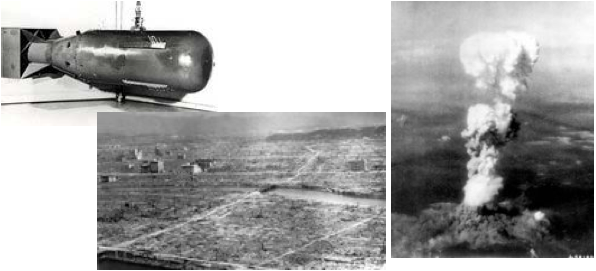
\includegraphics[width=75mm]{chap-0/nuclearbom.png}
\end{center}
\end{figure}
\end{column}
\end{columns}
}

\frame{
\begin{block}{In order to develope nuclear weapons,} 
\begin{itemize}
\item in 1950, only 15 computers worldwide; 
\item to September 1962,  there are 16,187 computers in the U.S. alone\footnote{由于核武器研制需要,1950年全球只有15台计算机,到了1962年9月仅美国就有16187台计算机。}.
\end{itemize}
\end{block}
\begin{figure}
\begin{center}
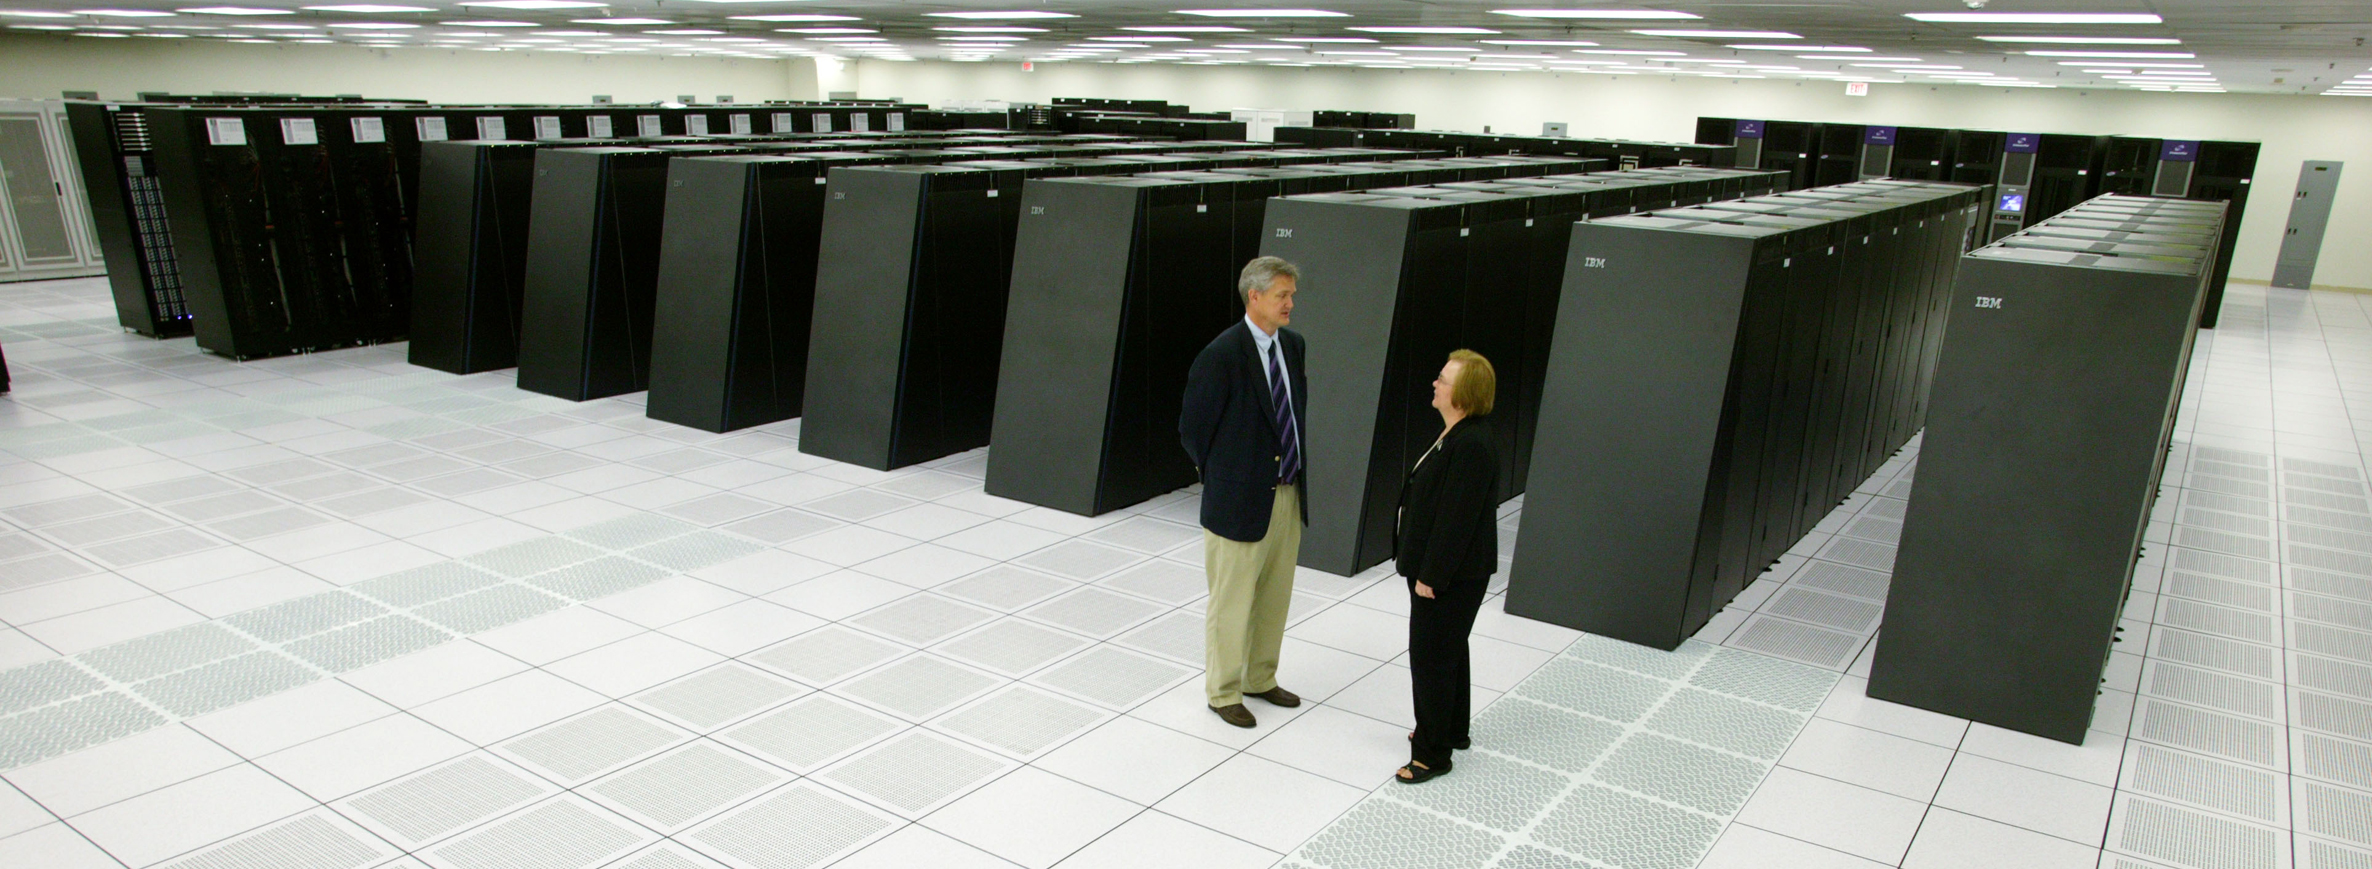
\includegraphics[width=95mm]{chap-0/BlueGene_big.jpg}
\begin{center}
\tiny{Livermore’s BlueGene/L supercomputer}
\end{center}
\end{center}
\end{figure}
}

%\frame{
%\frametitle{Supercomputer}
%\begin{figure}
%\begin{center}
%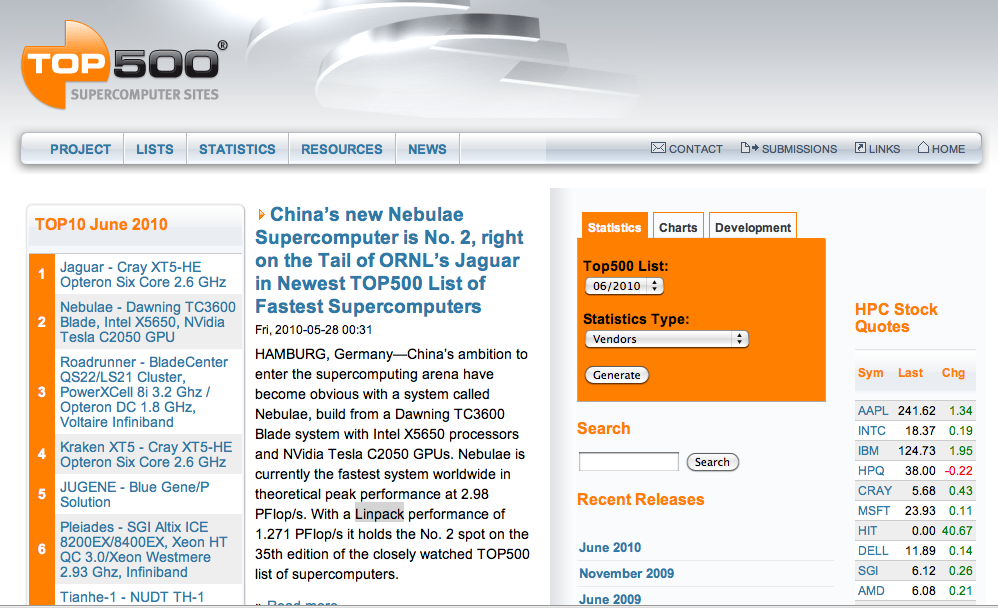
\includegraphics[width=110mm]{chap-0/top500.png} 
%\tiny{\\ Screenshots of "http://www.top500.org/" in Aug. 2010}
%\end{center}
%\end{figure}
%}

%\frame{
%\frametitle{Nebulae Supercomputer}
%\framesubtitle{星云超级计算机}
%\begin{figure}
%\begin{center}
%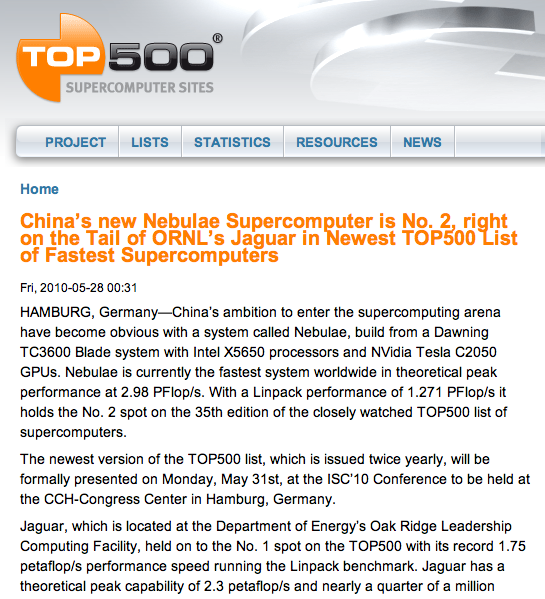
\includegraphics[width=60mm]{chap-0/top500-2.png} 
%\tiny{\\ Screenshots of "http://www.top500.org/lists/2010/06/press-release"}
%\end{center}
%\end{figure}
%}

\frame{
\begin{center}
\huge{
In order to apply the computing power to the solution of practical problems,  \\
the more efficient calculation method must be considered. \\
\vspace{0.2cm}
\begin{block}{}
In other word, \\
The numerical methods is very important\footnote{要把计算机强大的计算能力应用到实际问题的解决上, 必须要有高效的计算方法!}!
\end{block}
}
\end{center}
}

\frame{
\frametitle{Purpose of this Course}
%\framesubtitle{本课程的目的}
\begin{block}{Introduce computer methods for the solution of civil engineering problems, including:}
\begin{itemize}
\item General Introduction to Computer Applications in Engineering and Construction
\item Why do you need to be able to write and understand computer program and numerical methods?
\item Matlab - Mathematical Laboratory
\end{itemize}
\end{block}
\begin{block}{}
\begin{itemize}
\item Enable you to explore in-depth some aspect of Civil, Architectural, or Environmental Engineering of particular interest to you 
\item Provide experience in
\begin{itemize}
\item use of computer methods to solve engineering problems 
\item formulation, execution and presentation of an engineering investigation 
\end{itemize}
\end{itemize}
\end{block}
}

\frame{
\frametitle{Topics of this Course}
\begin{block}{}
\begin{itemize}
\item Fundamental Concepts of Numerical Methods
\begin{itemize}
\item Computer Errors $-$ Recognition and solutions 
\item Linear and Nolinear Algorithm $-$ Setting up multiple sets of equations and solution techniques
\item LU Decomposition (LU分解) $-$ Technique to decompose matrices
\item Eigen-analysis and Eigenvectors $-$ finding the eigenvalues and eigenvectors
\item Interpolation, Polynomial Approximation $\&$ Curve Fitting
\item Numerical Differention $\&$ Integration
\item ODE’s (ordinary differential equations) $-$ Initial Value Problems, Systems of ODE’s of IVP, Boundary Value Problems, Systems of ODE’s of BVP
\item Solution of Differential Equations $\&$ Partial Differential Equations (PDE’s)
\end{itemize}
\item Mathematical Software $\&$ Programming
\begin{itemize}
\item Matlab, Octave, Scilab
%\item C, Java
\end{itemize}
\end{itemize}
\end{block}
}



\frame{
\frametitle{Why do we need to know how to use numerical analysis and methods?}
\begin{block}{You are not going to be given a nice neat exact solution in the “real world”.} 
\begin{itemize}
\item Applications
\item Numerical Errors
\item Computer Types
\item Computer Software
\end{itemize}
\end{block}
}

\frame{
\begin{block}{Applications}
\begin{itemize}
\item Signal Processing
\item CFD (Computational Fluid Dynamics)
\item Structural Analysis
\item Finite Element Analysis
\item Interpolation $-$ Handling data
\item Optimization $-$ Design and estimation
\item CAD (Computer Aided-Drafting) 
\item Data Collection 
\end{itemize}
\end{block}
}

%\frame{
%\begin{block}{Computer  Hardware Types}
%\begin{itemize}
%\item Personal Computer
%\vspace{5mm}
%\item Supercomputers
%\vspace{5mm}
%\item Vector Processors
%\vspace{5mm}
%\item Array Processors
%\vspace{5mm}
%\item Parallel Processor
%\end{itemize}
%\end{block}
%}

%\frame{
%\frametitle{Software}
%\begin{block}{Operating Systems(OS)}
%\begin{itemize}
%\item Windows $-$ Windows XP, Vista, Windows 7
%\item Unix
%\item VMS $-$ VAX
%\item Linux 
%\end{itemize}
%\end{block}
%\begin{block}{Languages}
%\begin{itemize}
%\item Fundamental  Assembler (Bit manipulations)
%\item Engineering Languages
%\begin{itemize}
%\item Fortran, Cobol, Pascal
%\item C++  ( J++ )
%\item Basic
%\end{itemize}
%\item HTML and Java
%\end{itemize}
%\end{block}
%}

%\frame{
%\frametitle{Software}
%\begin{block}{Higher$-$Order Programming}
%\begin{itemize}
%\item Maple $-$ Mathematical Programming Language
%\item Mathematica $-$ Mathematical Programming Language
%\item Java $-$ Internet Programming Language
%\item Matlab $-$ Matrix Laboratory  
%\end{itemize}
%\end{block}
%\begin{block}{Tools}
%\begin{itemize}
%\item Word Processors
%\item Spreadsheets
%\item Database Management
%\item Graphics
%\item Mathematical Computer Codes
%\end{itemize}
%\end{block}
%}

%\frame{
%\begin{block}{What is a program?}
%Program consist of three main components:
%\vspace{0.3cm}
%\begin{itemize}
%\item {\huge Input}
% \vspace{0.3cm}
%\item {\huge Main Program} $-$ Numerical methods and analysis and/or evaluation.
%\vspace{0.3cm}
%\item {\huge Output} $-$ Results.
%\end{itemize} 
%\end{block}
%}

%\frame{
%\begin{block}{Inputs}
%\vspace{0.3cm}
%\begin{itemize}
%\item {\huge Numerical values} 
%\vspace{0.3cm}
%\item {\huge Initialization of the variables}
%\vspace{0.3cm}
%\item {\huge Conditions}
%\vspace{0.3cm}
%\item {\huge Equations}
%\end{itemize}
%\end{block}
%}

%\frame{
%\begin{block}{Main Program }
%Using flow charts, the programs can be designed to perform a task. Using :
%\vspace{0.3cm}
%\begin{itemize}
%\item {\huge Loops}    ($for, do \ldots while$)
%\vspace{0.3cm}
%\item {\huge Conditions} ($if \ldots then \ldots elseif \ldots$, etc$\ldots$ )
%\vspace{0.3cm}
%\item {\huge Error Convergence}  ($while$ )
%\end{itemize}
%\end{block}
%}

%\frame{
%\begin{block}{Outputs .}
% Outputs are the results of the program.  They can go through a series of post-processing methods
%\vspace{0.3cm}
%\begin{itemize}
%\item {\huge Numerical Values}
%\vspace{0.3cm}
%\item {\huge Decisions}
%\vspace{0.3cm}
%\item {\huge Graphs and Plots}
%\end{itemize}
%\end{block}
%}


%\setcounter{section}{-1}



\section{Preliminaries(预备知识)}

\frame{
\frametitle{Derivative $\&$ Antiderivative}
\framesubtitle{导数和不定积分}
\begin{block}{Consider the function $f(x) = \cos(x)$, }
\begin{itemize}
\item its derivative $f′(x) = - \sin(x)$, 
\item and its antiderivative $F(x) = \sin(x) + C$. 
\end{itemize}
\end{block}
\begin{block}{These formulas were studied in calculus.}
\begin{itemize}
\item The former is used to determine the slope $m = f'(x_0)$ of the curve $y = f (x)$ at a point $(x_0, f(x_0))$;
\item The latter is used to compute the area under the curve for $a \le x \le b$.
\end{itemize}
\end{block}
}

\frame{
 \begin{itemize}
\item The slope at the point $(\pi \slash 2, 0)$ is $m = f'(\pi \slash 2) = −1$ and can be used to find the tangent line at this point :
\begin{equation*}
y_{tan} = m\left( x - \frac{\pi}{2}\right) + 0 
= f' \left(\frac{\pi}{2} \right)\left(x-\frac{\pi}{2} \right)
= -x + \frac{\pi}{2}
\end{equation*}
\item The area under the curve for $ 0 \le x \le \pi \slash 2$ is computed using an integral :
\begin{equation*}
area = \int_0^{\pi \slash 2} \cos (x) dx
= F \left( \pi \slash 2 \right) -F(0) = \sin\left( \frac{\pi}{2} \right) - 0 
= 1 
\end{equation*}
\end{itemize}
\begin{columns}
\begin{column}{0.5\textwidth}
\begin{figure}
\begin{center}
\includegraphics[width=40mm]{chap-0/fig_1-1.png}
{\tiny  \\ The tangent line to the curve $y = cos(x)$ at the point $(\pi \slash 2, 0)$.}	
\end{center}
\end{figure}
\end{column}
\begin{column}{0.5\textwidth}
\begin{figure}
\begin{center}
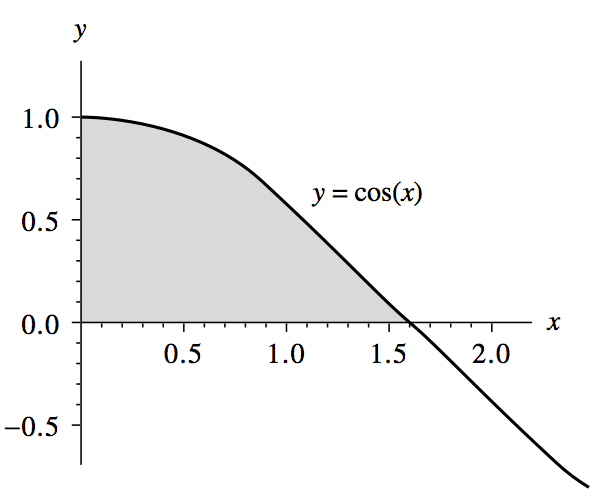
\includegraphics[width=40mm]{chap-0/fig_1-1_2.png}
{\tiny  \\ The area under the curve 
$y = \cos(x)$ 
over the interval
$[ 0, \pi \slash 2 ]$.}
\end{center}
\end{figure}
\end{column}
\end{columns}
}


\subsection{Review of Calculus}

\frame{
\begin{block}{}
\begin{itemize}
\item It is assumed that the reader is familiar with the notation and subject matter covered in the undergraduate calculus sequence. 
\vspace{0.5cm}
\item This should have included the topics :
\vspace{0.2cm}
\begin{itemize} 
\item limits (极限), 
\vspace{0.2cm}
\item continuity (连续), 
\vspace{0.2cm}
\item differentiation (微分), 
\vspace{0.2cm}
\item integration (积分), 
\vspace{0.2cm}
\item sequences (序列), 
\vspace{0.2cm}
\item series (级数).  
\end{itemize}
\end{itemize}
\end{block}
}

\frame{
\frametitle{Limits and Continuity}
\framesubtitle{极限和连续}
\begin{figure}
\begin{center}
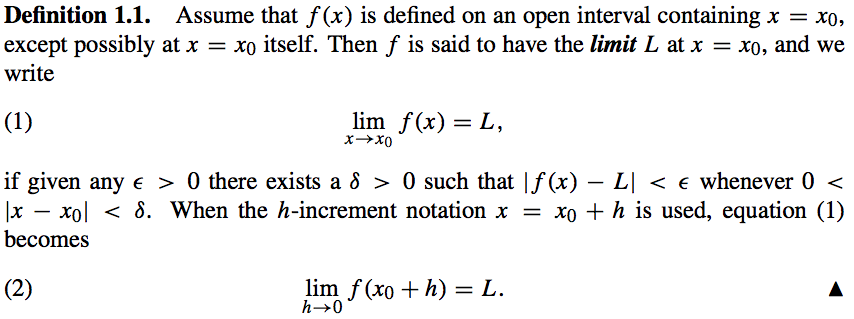
\includegraphics[width=115mm]{chap-0/def_1-1.png}
\end{center}
\end{figure}
\begin{block}{极限的定义}
例如,该定义主要是应用在本课程的非线性方程的迭代算法。
\end{block}
}

\frame{
\begin{figure}
\begin{center}
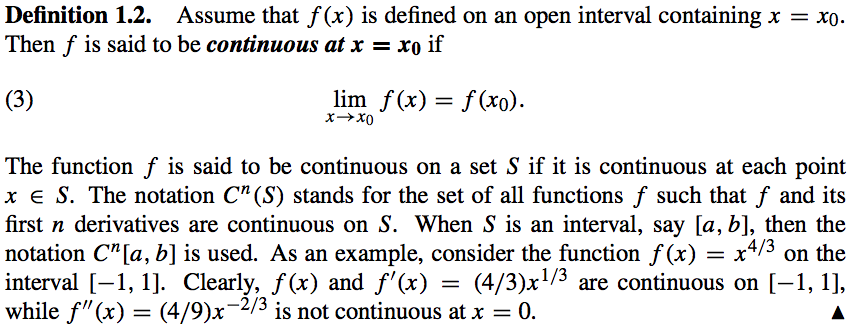
\includegraphics[width=115mm]{chap-0/def_1-2.png}
\end{center}
\end{figure}
\begin{block}{连续的定义}
注意与本课程之中所应用的离散数据的相似性和差别。
\end{block}
}

\frame{
\begin{figure}
\begin{center}
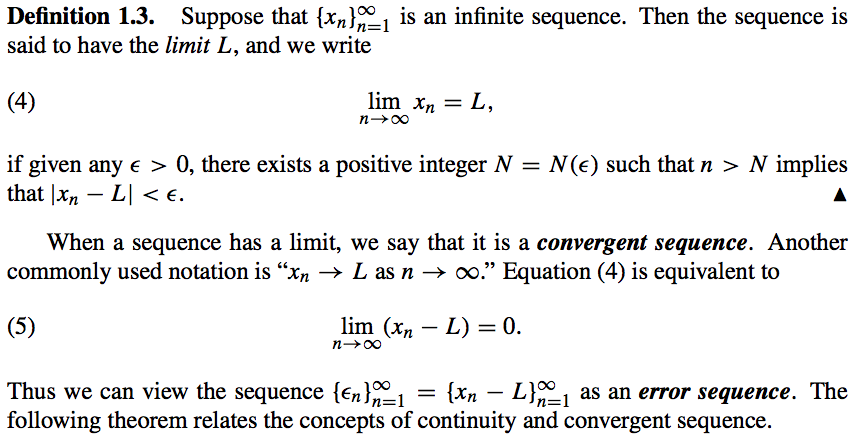
\includegraphics[width=115mm]{chap-0/def_1-3.png}
\end{center}
\end{figure}
\begin{block}{序列的收敛性定义}
由于计算机的数据存储是离散的,该定义在本课程之中具有实际意义。
\end{block}
}

\frame{
\begin{figure}
\begin{center}
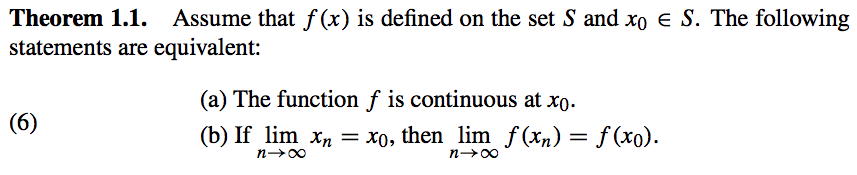
\includegraphics[width=115mm]{chap-0/the_1-1.png}
\end{center}
\end{figure}
\begin{block}{}
%由于计算机的数据存储是离散的,该定义在本课程之中具有实际意义。
\end{block}

\begin{figure}
\begin{center}
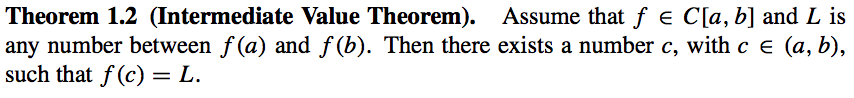
\includegraphics[width=115mm]{chap-0/the_1-2.png}
\end{center}
\end{figure}
\begin{block}{}
\end{block}
}

\frame{
\begin{figure}
\begin{center}
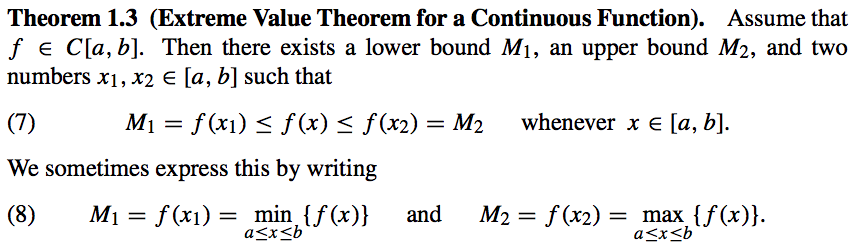
\includegraphics[width=115mm]{chap-0/the_1-3.png}
\end{center}
\end{figure}
\begin{block}{连续函数的极值定理}
\end{block}
}

\frame{
\frametitle{Differentiable Functions}
\framesubtitle{可微函数}
\begin{figure}
\begin{center}
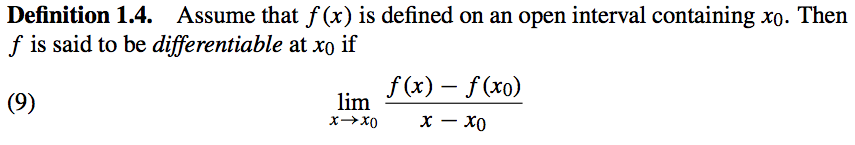
\includegraphics[width=115mm]{chap-0/def_1-4.png}
\end{center}
\end{figure}
\begin{figure}
\begin{center}
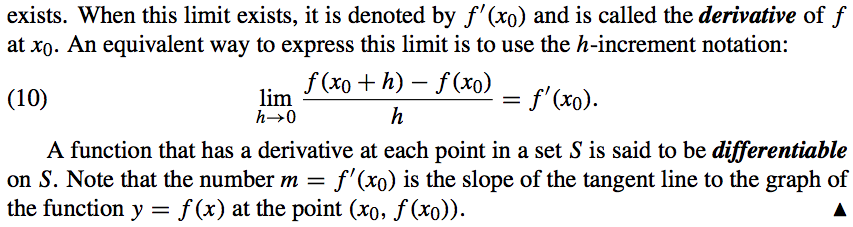
\includegraphics[width=115mm]{chap-0/def_1-4_2.png}
\end{center}
\end{figure}
\begin{block}{函数可导的定义}
可以利用该定义计算函数曲线的微分曲线。
\end{block}
}

\frame{
\begin{figure}
\begin{center}
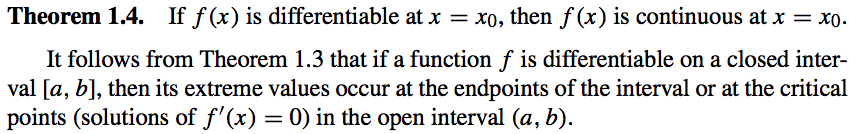
\includegraphics[width=115mm]{chap-0/the_1-4.png}
\end{center}
\end{figure}
\begin{block}{可导和连续的关系}
\begin{itemize}
\item 如果函数在指定点可导的话一定连续,
\item 但如果函数在指定点连续的话不一定可导
\end{itemize}
\end{block}
}

\frame{
\begin{figure}
\begin{center}
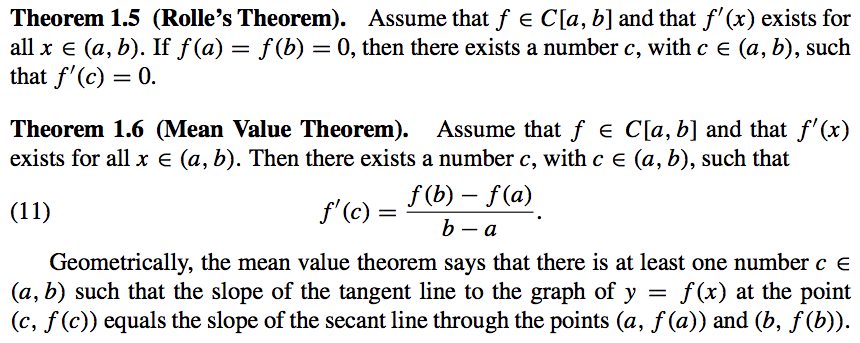
\includegraphics[width=115mm]{chap-0/the_1-5.png}
\end{center}
\end{figure}
\begin{block}{Rolle's theorem(罗尔定理) 和均值定理}
该定理可用在数值积分的推导之中
\end{block}
}

\frame{
\begin{figure}
\begin{center}
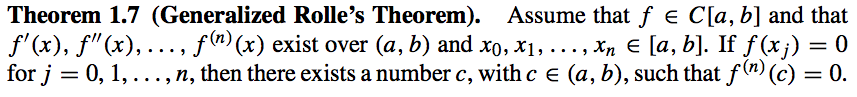
\includegraphics[width=115mm]{chap-0/the_1-7.png}
\end{center}
\end{figure}
\begin{block}{Generalized Rolle's theorem(广义罗尔定理) }
该定理是微分中值定理中最基本、最重要的,其证明具有广泛的代表性。
\end{block}
}

\frame{
\frametitle{Integrals}
\framesubtitle{积分}
\begin{figure}
\begin{center}
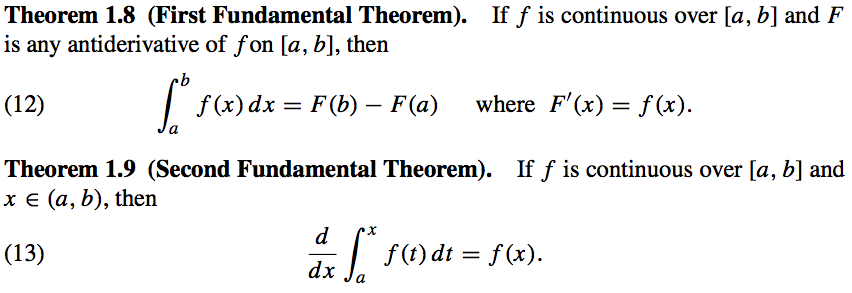
\includegraphics[width=115mm]{chap-0/the_1-8.png}
\end{center}
\end{figure}
\begin{block}{积分第一定理和第二定理}
该定理被应用在在本课程的数值积分。
\end{block}
}

\frame{
\begin{figure}
\begin{center}
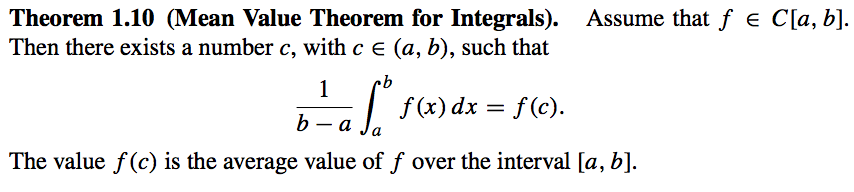
\includegraphics[width=115mm]{chap-0/the_1-10.png}
\end{center}
\end{figure}
\begin{block}{积分中值定理}
\end{block}
\begin{figure}
\begin{center}
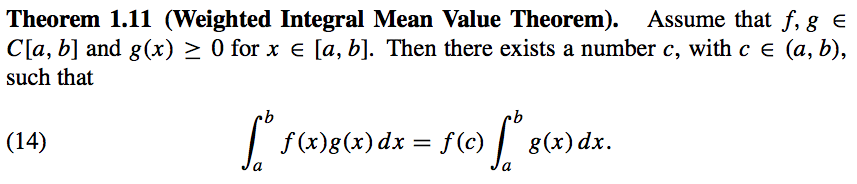
\includegraphics[width=115mm]{chap-0/the_1-11.png}
\end{center}
\end{figure}
\begin{block}{积分加权中值定理}
\end{block}
}

\frame{
\frametitle{Series}
\framesubtitle{级数}
\begin{figure}
\begin{center}
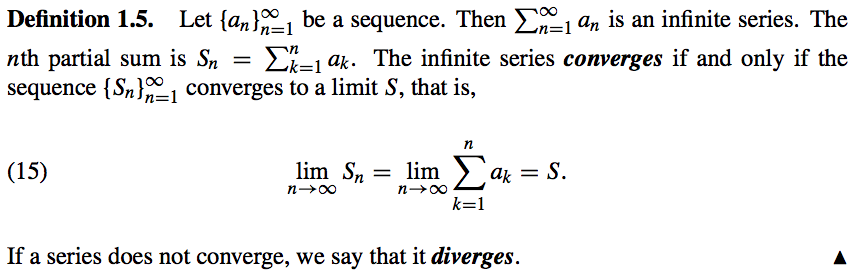
\includegraphics[width=115mm]{chap-0/def_1-5.png}
\end{center}
\end{figure}
\begin{block}{}
收敛和发散的定义
\end{block}
}

\frame{
\frametitle{Taylor's Theorem}
\framesubtitle{泰勒定理}
\begin{figure}
\begin{center}
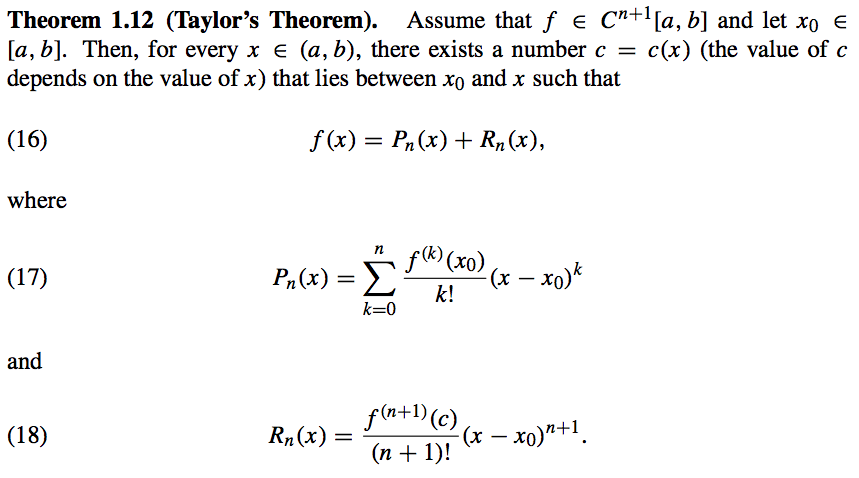
\includegraphics[width=115mm]{chap-0/the_1-12.png}
\end{center}
\end{figure}
}

\frame{
\frametitle{Corollary of the Taylor's Theorem}
\framesubtitle{泰勒定理的推理}
\begin{figure}
\begin{center}
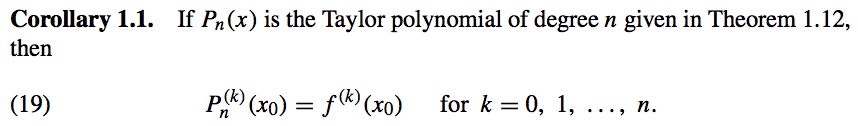
\includegraphics[width=115mm]{chap-0/coro_1-1.png}
\end{center}
\end{figure}
}

\frame{
\frametitle{Evaluation of a Polynomial}
\framesubtitle{多项式估值}
\begin{figure}
\begin{center}
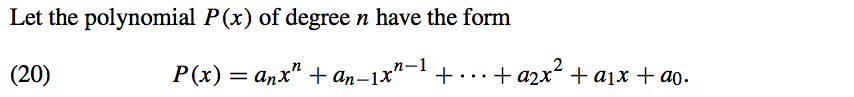
\includegraphics[width=115mm]{chap-0/p_19.png}
\end{center}
\end{figure}
\begin{figure}
\begin{center}
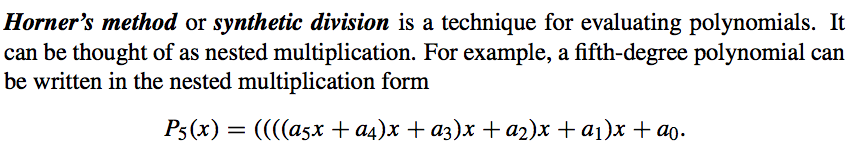
\includegraphics[width=115mm]{chap-0/p_19_2.png}
\end{center}
\end{figure}
}

\frame{
\begin{figure}
\begin{center}
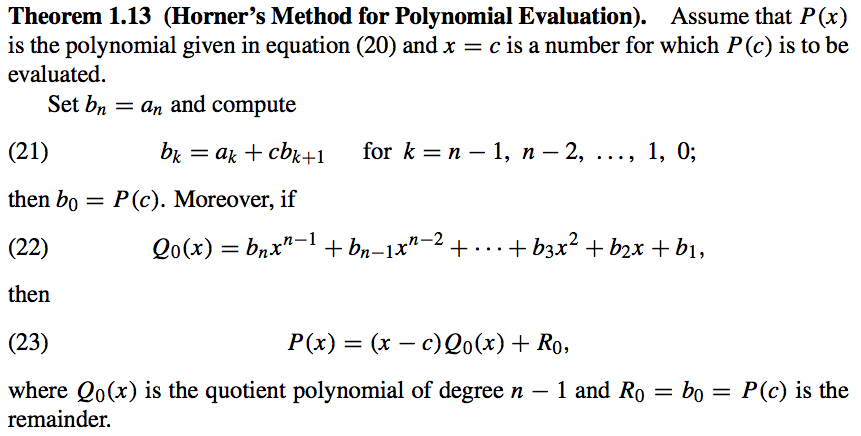
\includegraphics[width=115mm]{chap-0/the_1-13.png}
\end{center}
\end{figure}
}

\frame{
\begin{figure}
\begin{center}
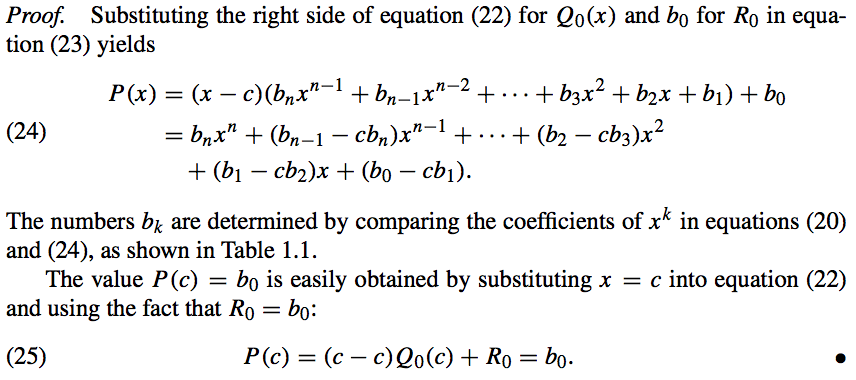
\includegraphics[width=115mm]{chap-0/the_1-13_2.png}
\end{center}
\end{figure}
}



\subsection{Binary Numbers(二进制数)}

\frame{
\begin{block}{}
\begin{itemize}
\item Human beings do arithmetic using the decimal (base 10) number system. 
\item Most computers do arithmetic using the binary (base 2) number system. 
\end{itemize}
\end{block}
\begin{itemize}
\item It may seem otherwise, 
since communication with the computer (input/output) is in base 10 numbers. 
\item This transparency does not mean that the computer uses base 10. 
\item In fact, it converts inputs to base 2 (or perhaps base 16), then performs base 2 arithmetic, and finally, translates the answer into base 10 before it displays a result. 
\end{itemize}
}

\frame{
\frametitle{Base 10 Number}
\begin{figure}
\begin{center}
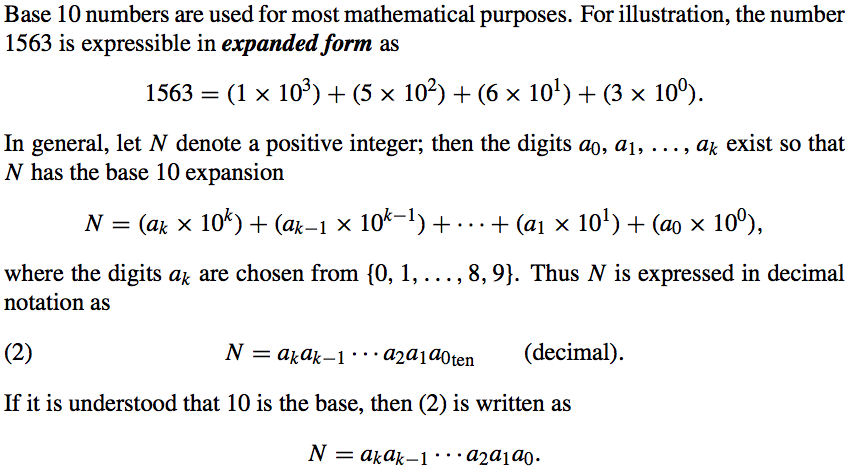
\includegraphics[width=115mm]{chap-0/p_24.png}
\end{center}
\end{figure}
}

\frame{
\frametitle{Base 2 Number}
\begin{figure}
\begin{center}
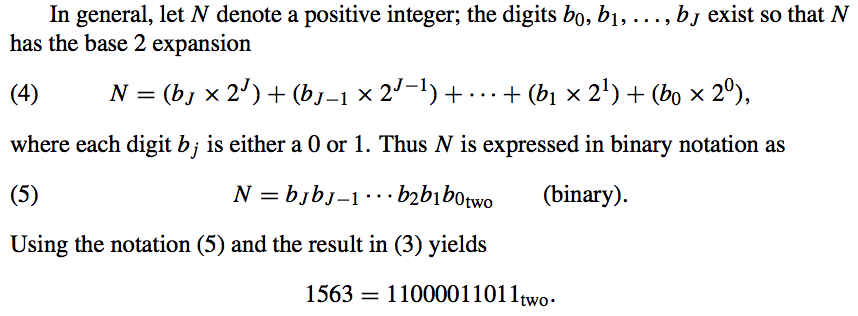
\includegraphics[width=115mm]{chap-0/p_24_2.png}
\end{center}
\end{figure}
}

\frame{
\frametitle{Sequences and Series}
\begin{figure}
\begin{center}
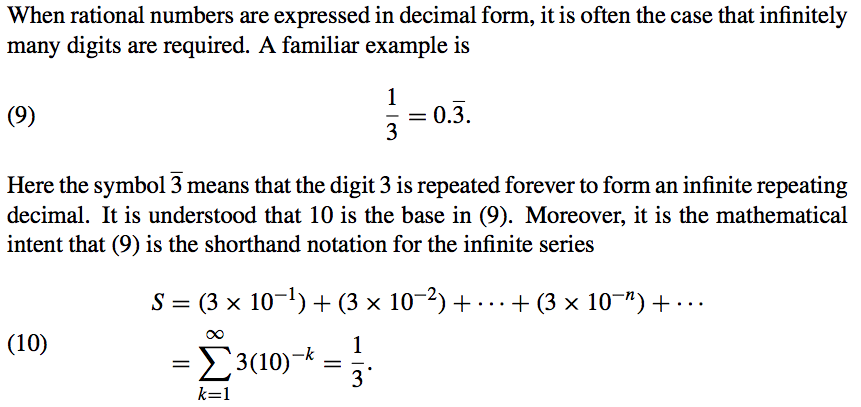
\includegraphics[width=115mm]{chap-0/p_26.png}
\end{center}
\end{figure}
}

\frame{
\begin{figure}
\begin{center}
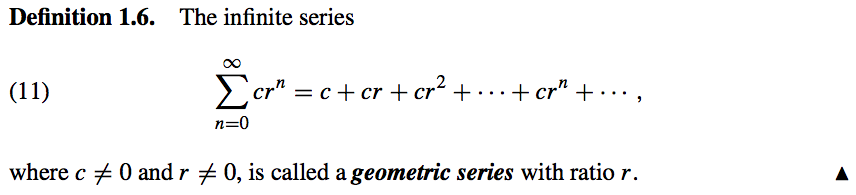
\includegraphics[width=115mm]{chap-0/def_1-6.png}
\end{center}
\end{figure}
\begin{figure}
\begin{center}
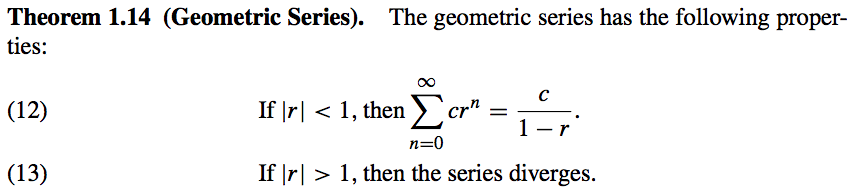
\includegraphics[width=115mm]{chap-0/the_1-14.png}
\end{center}
\end{figure}
}

%\frame{
%\frametitle{Computer Accuracy}
%\framesubtitle{计算机精度}
%\begin{itemize}
%\itemTo store numbers accurately, computers must have floating-point binary numbers %with at least 24 binary bits used for the mantissa; 
%\item this translates to about seven decimal places. 
%\item If a 32-bit mantissa is used, numbers with nine decimal places can be stored. 
%\end{itemize}
%}





\subsection{Error Analysis(误差分析)}

\frame{
\begin{block}{Error Analysis}
\begin{itemize}
\item In the practice of numerical analysis it is important to be aware that computed solutions are not exact mathematical solutions. 
\vspace{0.3cm}
\item The precision of a numerical solution can be diminished in several subtle ways. 
\vspace{0.3cm}
\item Understanding these difficulties can often guide the practitioner in the proper implementation and/or development of numerical algorithms.
\end{itemize}
\end{block}
}

\frame{
\begin{center}
{\Huge Computers are only as good as the person running them.}
\end{center}
}

\frame{
\frametitle{Numerical Errors}
\begin{itemize}
\item Precision Limits(精度限制)
\item Stability
\begin{itemize}
\item Convergence(收敛)
\item Divergence (发散)
\end{itemize}
\item Round-off Errors
\item Truncation Errors $-$ Code dependent
\item Machine Precision
\end{itemize}
\begin{block}{误差来源}
\begin{itemize}
\item 模型误差: 在建立数学模型过程中,不可能将所有因素均考虑,必然要进行必要的简化,这就带来了与实际问题的误差。
\item 观测误差: 测量已知参数时,数据带来的误差。工程问题的参数包含有不可避免的测量误差。
\item 截断误差:数值方法的精确解与待求解模型的理论分析解之间的差异
\item 舍入误差:对超过某有限位数的数据进行舍入所产生的误差
\end{itemize}
\end{block}
}

\frame{
\frametitle{Absolute $\&$ Relative errors}
\framesubtitle{绝对误差和相对误差}
\begin{figure}
\begin{center}
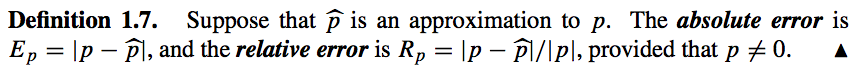
\includegraphics[width=115mm]{chap-0/def_1-7.png}
\end{center}
\end{figure}
\begin{block}{Example}
Let $x = 3.141592$ and $ \hat{x} = 3.14 $
\begin{itemize}
\item $ E_x = |x - \hat{x}| = |3.141592 - 3.14| = 0.001592 $
\vspace{0.3cm}
\item $ R_x = \frac{|x - \hat{x}|}{|x|}  = \frac{0.001592}{3.141592} = 0.00507 $
\end{itemize}
\end{block}
}

\frame{
\frametitle{Truncation Error}
\framesubtitle{截断误差}
\begin{figure}
\begin{center}
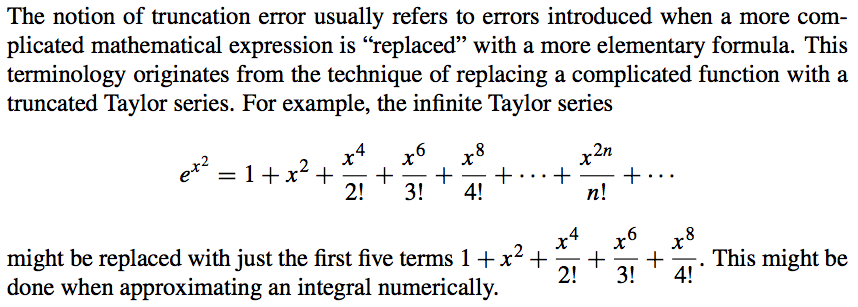
\includegraphics[width=115mm]{chap-0/p_36.png}
\end{center}
\end{figure}

}

\frame{
\frametitle{Round-off Error}
\framesubtitle{舍入误差}
\begin{block}{}
\begin{itemize}
\item A computer’s representation of real numbers is limited to the fixed precision of the mantissa. 
\item True values are sometimes not stored exactly by a computer’s represen- tation. This is called round-off error.
\end{itemize}
\end{block}
\begin{block}{}
\begin{itemize}
\item In the preceding section the real number $1/10 = 0.0\bar{0011}_{two} $ was truncated when it was stored in a computer. 
\item The actual number that is stored in the computer may undergo chopping or rounding of the last digit. 
\item Therefore, since the computer hardware works with only a limited number of digits in machine numbers, rounding errors are introduced and propagated in successive computations.
\end{itemize}
\end{block}
}

\frame{
\frametitle{误差界 $\&$ 误差限}
\begin{block}{}
设$x$为准确值,
$x^{\ast}$为$x$的一个近似值,
若
\begin{equation*}
| e | = | x - x^{\ast} | \le  \epsilon
\end{equation*}
则$\epsilon$为$x^{\ast}$的绝对误差界,简称误差界。\\
若
\begin{equation*}
|e_r| = \frac{| x - x^{\ast} |}{| x^{\ast} |}  \le  \epsilon_r
\end{equation*}
则$\epsilon_r$为$x^{\ast}$的相对误差界。\\
\end{block}
\begin{block}{}
引入$\epsilon$误差界的定义,可以把无法明明白白写出来得准确值$x$表示为:
\begin{equation*}
 x^{\ast}  - \epsilon  \le  x  \le  x^{\ast}  + \epsilon
\hspace{1cm} 或 \hspace{1cm} 
x  =   x^{\ast}  \pm \epsilon
\end{equation*}
\end{block}
}

\frame{
\frametitle{Significant digits}
\framesubtitle{有效数字}
\begin{figure}
\begin{center}
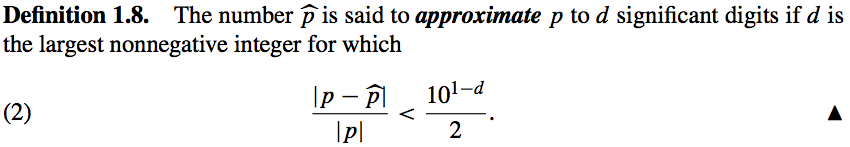
\includegraphics[width=115mm]{chap-0/def_1-8.png}
\end{center}
\end{figure}
\begin{block}{Example}
If $x = 3.141592$ and $\hat{x} = 3.14$,  \\
then $\frac{|x - \hat{x}|}{|x|} = 0.000507 < \frac{10^{-2}}{2}$. \\
Therefore, $\hat{x}$ approximates $x$ to two significant digits.
\end{block}
}



\frame{
\frametitle{Loss of Significance}
\framesubtitle{精度损失}
Consider the two numbers $p = 3.1415926536$ and $q = 3.1415957341$, which are nearly equal and both carry 11 decimal digits of precision. 
\begin{itemize}
\item Suppose that their difference is formed: $p - q = −0.0000030805$. 
\item Since the first six digits of $p$ and $q$ are the same, their difference $p - q$ contains only five decimal digits of precision. 
\item This phenomenon is called loss of {\large significance} or {\large subtractive cancellation}. 
\item This reduction in the precision of the final computed answer can creep in when it is not suspected.
\end{itemize}
\begin{block}{}
For polynomial evaluation, the rearrangement of terms into nested multiplication form will sometimes produce a better result.
\end{block}
}

\frame{
\frametitle{$O(h^n)$ Order of Approximation}
\framesubtitle{$O(h^n)$阶逼近}
\begin{figure}
\begin{center}
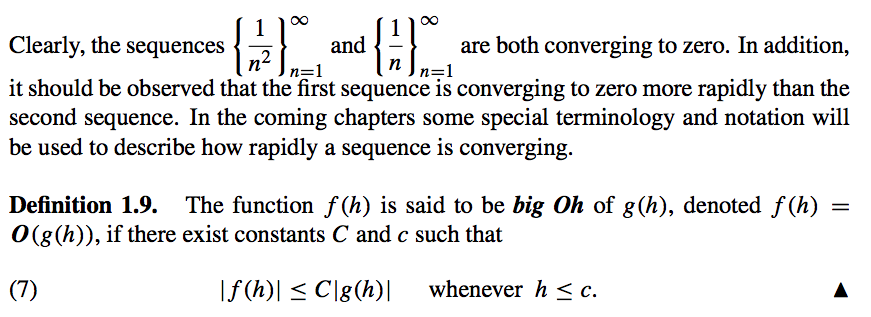
\includegraphics[width=115mm]{chap-0/def_1-9.png}
\end{center}
\end{figure}
}

\frame{
\frametitle{$O(h^n)$ Order of Approximation}
\framesubtitle{$O(h^n)$阶逼近}
\begin{figure}
\begin{center}
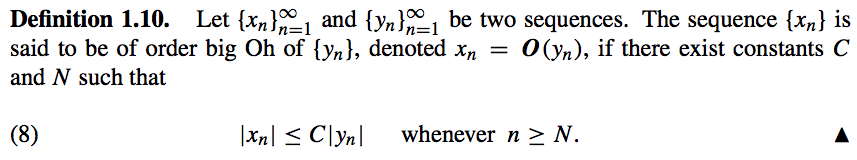
\includegraphics[width=115mm]{chap-0/def_1-10.png}
\end{center}
\end{figure}
\begin{figure}
\begin{center}
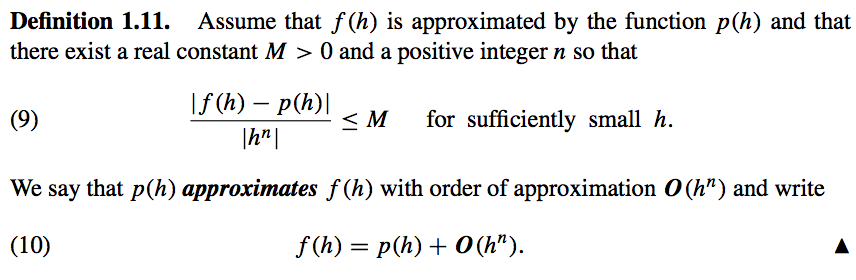
\includegraphics[width=115mm]{chap-0/def_1-11.png}
\end{center}
\end{figure}
}

\frame{
\begin{figure}
\begin{center}
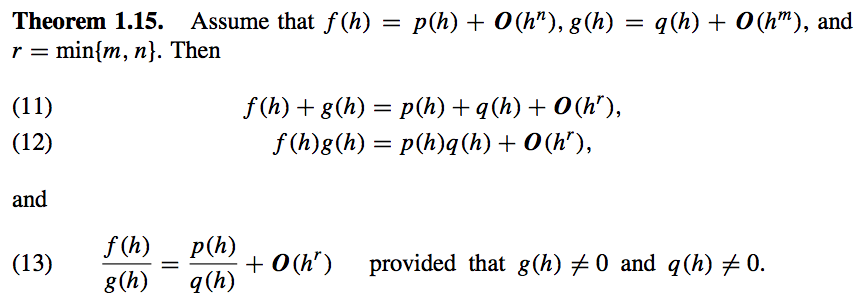
\includegraphics[width=115mm]{chap-0/the_1-15.png}
\end{center}
\end{figure}
\begin{figure}
\begin{center}
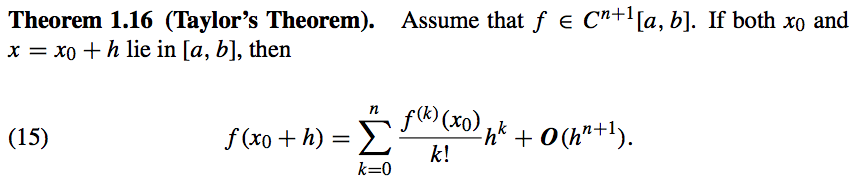
\includegraphics[width=115mm]{chap-0/the_1-16.png}
\end{center}
\end{figure}
}


\frame{
\frametitle{Order of Convergence of a Sequence}
\begin{itemize}
\item Numerical approximations are often arrived at by computing a sequence of approximations that get closer and closer to the answer desired. 
\item The definition of big $Oh$ for sequences was given in Definition 1.10, and the definition of order of convergence for a sequence is analogous to that given for functions in Definition 1.11.
\end{itemize}
\begin{figure}
\begin{center}
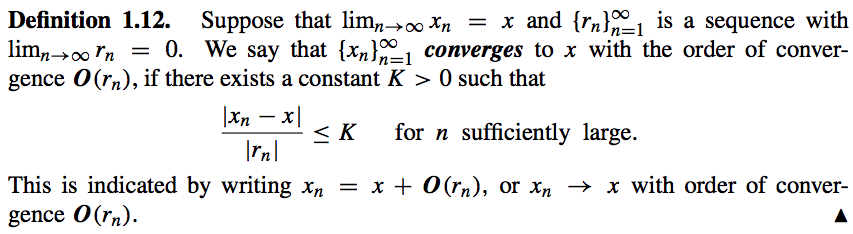
\includegraphics[width=115mm]{chap-0/def_1-12.png}
\end{center}
\end{figure}
}



\frame{
\frametitle{Uncertainty in Data}
\begin{itemize}
\item Data from real-world problems contain uncertainty or error. 
\item This type of error is referred to as noise. 
\item It will affect the accuracy of any numerical computation that is based on the data. 
\item An improvement of precision is not accomplished by performing succes- sive computations using noisy data. 
\item Hence, if you start with data with d significant digits of accuracy, then the result of a computation should be reported in d significant digits of accuracy. 
\end{itemize}
}

\frame{
For example,
\begin{itemize}
\item suppose that the data $p_1 = 4.152$ and $p_2 = 0.07931$ both have four significant digits of accuracy. 
\item Then it is tempting to report all the digits that appear on your calculator (i.e., $p_1 + p_2 = 4.23131$). 
\item This is an oversight, because you should not report conclusions from noisy data that have more significant digits than the original data. 
\item The proper answer in this situation is $p_1 + p_2 = 4.231$.
\end{itemize}
}


\subsection{Matlab $-$ Matrix Laboratory}

\frame{
\frametitle{Matlab的起源}
\begin{itemize}
\item 20世纪七十年代,时任美国新墨西哥大学计算机科学系主任的Cleve Moler出于减轻学生编程负担的动机, 为学生设计了一组调用LINPACK和EISPACK矩阵软件工具包库程序的的“通俗易用”的接口,此即用FORTRAN编写的萌芽状态的MATLAB。
\item 1984年由Little、Moler、Steve Bangert合作成立MathWorks公司,并把MATLAB正式推向市场。从这时起,MATLAB的内核采用C语言编写,而且除原有的数值计算能力外,还新增了数据图视功能。
\item 取名MATLAB即Matrix Laboratory 矩阵实验室的意 思。
\end{itemize}
}

\frame{
\frametitle{Matlab的特点}
\begin{itemize}
\item MATLAB是一种直译式的高级语言,比其它程序设计语言容易。
\item MATLAB语言是功能强大的计算机高级语言, 它以超群的风格与性能风靡全世界, 成功地应用于各工程学科的研究领域。 MATLAB在美国已经作为大学工科学生必修的计算机语言之一(C, FORTRAN, ASSEMBLER, MATLAB)。
\item MATLAB提供了丰富的矩阵运算处理功能,是基于矩阵运算的处理工具。
\end{itemize}
}

\frame{
\frametitle{主要应用领域}
\begin{itemize}
\item 工业研究与开发 ␣ 
\item 数学教学,特别是线性代数 
\item 数值分析、 信号处理和科学计算方面的教学与研究
\item 电子学、控制理论和物理学等工程和科学学科方面的教学与研究
\item 经济学、化学和生物学等计算问题的所有其他领域中的教学与研究
\end{itemize}
}


\frame{
%The Matlab program can be run using command line,  batch commands, and programs.
\begin{block}{Variable Types}
\begin{itemize}
\item Integers
\item Real Values (float and double)
\item Complex Numbers ($a + ib$)
\begin{itemize}
\item a $-$ real value
\item b $-$ imaginary value ($i$ is the square root of $-1$)   
\end{itemize}
\end{itemize}
\end{block}
\begin{block}{Data Types}
\begin{itemize}
\item Numerical
\begin{itemize}
\item Scalars
\item Vectors
\item Matrices
\end{itemize}
\item Logic Types
\item Alpha/Numerical Types
\end{itemize}
\end{block}
}

\frame{
\begin{itemize}
\item A scalar value is the simple number, $a$, $2$, $3.14157$ $\ldots$, 
\item A vector is a union of a
\end{itemize}
\begin{equation*}  
\bar{x} = \left\{ x_1, x_2, \ldots, x_n \right\} 
\end{equation*}
\begin{itemize}					
\item Transpose vector
\end{itemize}
\begin{equation*}
\bar{x}^T = \left\{
\begin{array}{c}
 x_1 \\
 x_2 \\
 \vdots \\
 x_n
\end{array} 
\right\}
\end{equation*}
}

\frame{
\begin{block}{Matrix is a combination of vectors and scalars.  Scalar and vectors are subsets of matrices.}
\begin{equation*}
A = \left[
\begin{array}{c c c c}
a_{11}  & a_{12}  & \cdots & a_{1n} \\
a_{21}  & a_{22}  & \cdots & a_{2n} \\
\vdots & \vdots & \ddots & \vdots \\ 
a_{n1}  & a_{n2}  & \cdots & a_{nn} \\
\end{array}
\right]
\end{equation*}
Matlab uses matrix to do mathematical methods.
\end{block}
}

\frame{
\begin{block}{Set of computer functions}
\begin{itemize}
\item Circular functions 
\begin{itemize}
\item $sin(x)$, $cos(x)$, $tan(x)$
\item $asin(x)$, $acos(x)$, $atan(x)$
\end{itemize}
\item Hyperbolic functions   
\begin{itemize}
\item $sinh(x)$, $cosh(x)$, $tanh(x)$
\end{itemize}
\item Logarithmic functions 
\begin{itemize}
\item $ln(x)$, $log(x)$ 
\item $exp(x)$
\end{itemize}
\item Logic functions           
\begin{itemize}
\item $abs(x)$
\item $real(x)$, $imag(x)$
\end{itemize}
\end{itemize}
\end{block}
}

\frame{
\begin{block}{Simple commands}
\begin{itemize}
\item clc     $-$ clears window
\item clg     $-$ clear graphic window
\item clear  $-$ clears the workspace
\item who	 $-$ variable list
\item whos $-$ variable list with size
\item help	 $-$ when doubt use it!
\end{itemize}
\end{block}
\begin{block}{Simple commands and symbols} 
\begin{itemize}
\item $^{\wedge}$C	$-$ an escape from a loop
\item inf	$-$ infinity
\item NaN	$-$ No numerical value
\end{itemize}
\end{block}
}

\frame{
\begin{block}{Scalar Operations}
\begin{itemize}
\item Addition          $-$ $a + b$
\item Subtraction     $-$ $a - b$
\item Multiplication $-$ $a \ast b$
\item Right Division $-$ $a \slash b$   
\item Left Division   $-$ $b \backslash a$ 
\item Exponential     $-$ $a ^{\wedge} b$
\end{itemize}
\end{block}
\begin{block}{}
$A \backslash B$ is the matrix division of $A$ into $B$, which is roughly the same as $INV(A) \ast B$ , except it is computed in a different way. 
If $A$ is an $N-by-N$ matrix and B is a column vector with $N$ components, or a matrix with several such columns, then $X = A \backslash B$ is the solution to the equation $A \ast X = B$ computed by Gaussian elimination. 
$A$ warning message is printed if $A$ is badly scaled or nearly singular. $A \backslash EYE(SIZE(A))$ produces the inverse of $A$.
\end{block}
}

\frame{
\frametitle{Order of Precedence of Arithmetic Operations}
\begin{block}{Precedence}
\begin{itemize}
\item ( 1 ) $-$ Parenthesis\footnote{括号}
\item ( 2 ) $-$ Exponential from left to right
\item ( 3 ) $-$ Multiplication and division from left to right.
\item ( 4 ) $-$ Addition and subtraction from left to right.  
\end{itemize}
\end{block}
}


%\setcounter{section}{0}



\section{Solution of Nonlinear Equations $f(x) = 0$}



\frame{
%\title{}
\begin{block}{A physical problem}
\begin{itemize}
\item  A spherical ball of radius $r$ is submerged to a depth $d$ in water. 
\item Assume that the ball is constructed from a variety of longleaf pine that has a density of $\rho = 0.638$ and that its radius measures $r = 10 cm$. 
\item How much of the ball will be submerged when it is placed in water?
\end{itemize}
\end{block}
\begin{figure}
\begin{center}
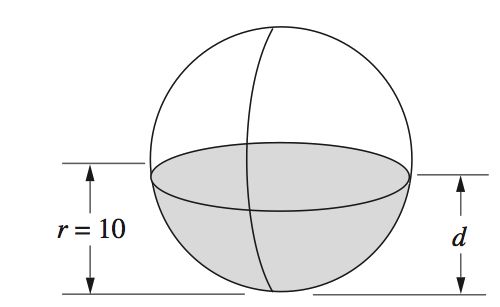
\includegraphics[width=45mm]{chap-1/fig_2-1.png}
%\includegraphics[width=45mm]{fig/ch-1/fig_1-1.png}
\caption{The portion of a sphere of radius $r$ that is to be submerged to a depth $d$}
\end{center}
\end{figure}
}

\frame{
%\begin{block}{}
\begin{itemize}
\item The mass $M_w$ of water displaced when a sphere is submerged to a depth $d$ is
\begin{equation*}
M_w = \int_0^d \pi (r^2 - (x-r)^2) dx = \frac{\pi d^2(3r-d)}{3}
\end{equation*}
\item the mass of the bell is 
\begin{equation*}
M_b = 4 \pi r^3 \rho \slash 3
\end{equation*}
\end{itemize}
%\end{block}
}

\frame{
\begin{columns}
\begin{column}{0.5\textwidth}
\begin{equation*}
\begin{array}{c}
M_w = M_b \\
\Downarrow \\
\frac{\pi(d^3 - 3d^2r + 4r^3 \rho)}{3} = 0 \\
\Downarrow \\
\frac{\pi(2552 - 30d^2 + d^3)}{3} = 0 \\
\Downarrow \\
y = 2552 -30d^2 + d^3
\end{array}
\end{equation*}
\end{column}
\begin{column}{0.5\textwidth}
\begin{figure}
\begin{center}
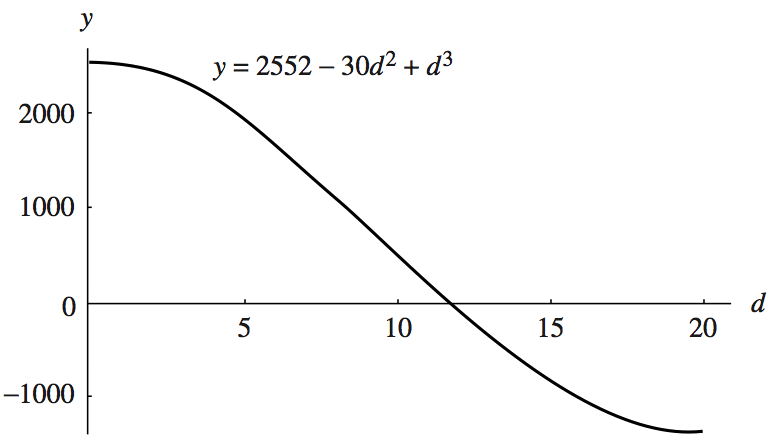
\includegraphics[width=45mm]{chap-1/fig_2-2.png}
%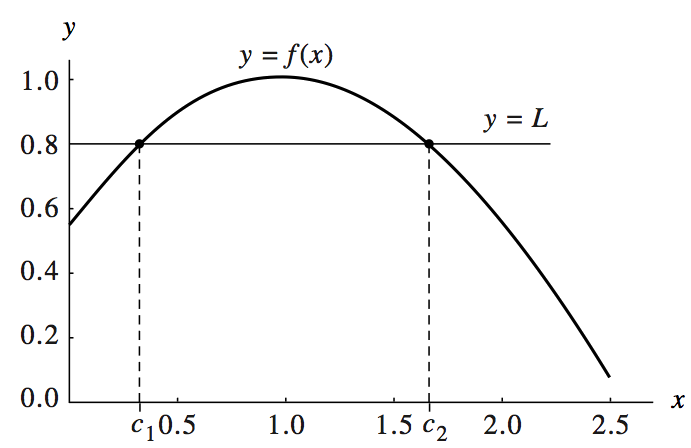
\includegraphics[width=55mm]{fig/ch-1/fig_1-2.png}
\caption{The cubic $y = 2552 - 30d^2 + d^3$}
\end{center}
\end{figure}
\end{column}
\end{columns}
\begin{center}
$\Downarrow $
\end{center}
\begin{block}{Solutions}
\begin{equation*}
\begin{array}{l l}
d_1 & = -8.17607212 \\
{\color{red} d_2} & {\color{red} = 11.86150151} \\
d_3 & = 26.31457061
\end{array}
\end{equation*}
\end{block}
}




\subsection{Bracketing Methods for Locating a Root}

\frame{
\frametitle{Consider a familiar topic of interest.}
Suppose that you save money by making regular monthly deposits $P$ and the annual interest rate is $I$; 
then the total amount $A$ after $N$ deposits is
\begin{equation*}
A = P + P(1+\frac{I}{12}) + P(1+\frac{I}{12})^2 + \cdots + P(1+\frac{I}{12})^{N-1}.
\end{equation*}
}

\frame{
\begin{itemize}
\item The first term on the right side of equation is the last payment. 
\item Then the next-to- last payment, which has earned one period of interest, contributes $P (1 + I /12)$. 
\item The second-from-last payment has earned two periods of interest and contributes $P (1 + I /12)^2$ , and so on. 
\item Finally, the last payment, which has earned interest for $N - 1$ periods, contributes $P (1 + I/12)^{N-1}$ toward the total. Recall that the formula for the sum of the $N$ terms of a geometric series is
\begin{equation*}
1 + r + r^2 + r^3 + \cdots + r^{N-1} = \frac{1-r^N}{1-r}
\end{equation*}
\end{itemize}
}

\frame{
We can write the amount $A$ equation  in the form
\begin{equation*}
A = P \left( 1+ (1 +\frac{I}{12}) + (1+\frac{I}{12})^2 + \cdots + (1+\frac{I}{12})^{N-1}  \right)
\end{equation*}
and use the substitution $r = (1 + I /12)$  to obtain
\begin{equation*}
A = P \frac{1 - \left(1 + \frac{I}{12}\right)^N}{1 - \left( 1 + \frac{I}{12} \right)}
\end{equation*}
This can be simplified to obtain the annuity-due equation,
\begin{equation*}
A = \frac{P}{\frac{I}{12}} \left( \left( 1 + \frac{I}{12} \right)^N - 1 \right)
\end{equation*}
}

\frame{
\begin{block}{Example.}
You save $\$250$ per month for $20$ years and desire that the total value of all payments and interest is $\$250, 000$ at the end of the $20$ years. What interest rate $I$ is needed to achieve your goal? 
\end{block}
If we hold $N = 240$ fixed, then $A$ is a function of $I$ alone; that is, $A = A(I)$. \\
We will start with two guesses, $I_0 = 0.12$ and $I_1 = 0.13$, and perform a sequence of calculations to narrow down the final answer. 
}

\frame{
Starting with $I_0 = 0.12$ yields
\begin{equation*}
A(0.12) = \frac{250}{0.12/12} \left( \left( 1 + \frac{0.12}{12} \right)^240 - 1\right) = 247,314
\end{equation*}
Since this value is a little short of the goal, we next try $I_1 = 0.13$:
\begin{equation*}
A(0.13) = \frac{250}{0.13/12} \left( \left( 1 + \frac{0.13}{12} \right)^240 - 1\right) = 282,311
\end{equation*}
This is a little high, so we try the value in the middle $I_2 = 0.125$:
\begin{equation*}
A(0.125) = \frac{250}{0.125/12} \left( \left( 1 + \frac{0.125}{12} \right)^240 - 1\right) = 264,623
\end{equation*}
}

\frame{
This is again high and we conclude that the desired rate lies in the interval $[0.12, 0.125]$. \\
The next guess is the midpoint $I_3 = 0.1225$:
\begin{equation*}
A(0.1225) = \frac{250}{0.1225/12} \left( \left( 1 + \frac{0.1225}{12} \right)^240 - 1\right) = 255,803
\end{equation*}
This is high and the interval is now narrowed to $[0.12, 0.1225]$. 
Our last calculation uses the midpoint approximation $I_4 = 0.12125$:
\begin{equation*}
A(0.12125) = \frac{250}{0.12125/12} \left( \left( 1 + \frac{0.12125}{12} \right)^240 - 1\right) = 251,518
\end{equation*}
}

\frame{
\begin{itemize}
\item Further iterations can be done to obtain as many significant digits as required.
\item The purpose of this example was to find the value of $I$ that produced a specified level $L$ of the function value, that is, to find a solution to $A(I) = L$. 
\item It is standard practice to place the constant $L$ on the left and solve the equation $A(I) - L = 0$.
\end{itemize}
}

\frame{
\begin{block}{Definition.}
Assume that $f (x)$ is a continuous function. Any number $r$ for which $f (r) = 0$ is called a {\Large root of the equation} $f (x) = 0$. 
Also, we say that $r$ is a {\Large zero of the function} f (x).
\end{block}
\vspace{0.5cm}
For example,\\
the equation $2x^2 + 5x - 3 = 0$ has two real roots $r_1 = 0.5$ and $r_2 = -3$, 
whereas the corresponding function $f (x) = 2x^2 +5x -3 = (2x -1)(x +3)$ has two real zeros, $r_1 = 0.5$ and $r_2 = -3$.
}

\frame{
\frametitle{Bisection Method of Bolzano}
\framesubtitle{The bracketing method for finding a zero of a continuous function}
\begin{itemize}
\item We must start with an initial interval $[a, b]$, where $f (a)$ and $f (b)$ have opposite signs. 
\vspace{0.3cm}
\item Since the graph $y = f (x)$ of a continuous function is unbroken, it will cross the $x -$ axis at a zero $x = r$ that lies somewhere in the interval. 
\vspace{0.3cm}
\item The bisection method systematically moves the endpoints of the interval closer and closer together until we obtain an interval of arbitrarily small width that brackets the zero.
\end{itemize}
}

\frame{
\begin{block}{The decision step for this process of interval halving is first to choose the midpoint $c = (a + b)/2$ and then to analyze the three possibilities that might arise:}
\begin{itemize}
\item If $f (a)$ and $f (c)$ have opposite signs, a zero lies in $[a, c]$. 
\item If $f (c)$ and $f (b)$ have opposite signs, a zero lies in $[c, b]$.
\item If $f(c) = 0$, then the zero is $c$.
\end{itemize}
\end{block}
\begin{columns}
\begin{column}{0.5\textwidth}
\begin{figure}
\begin{center}
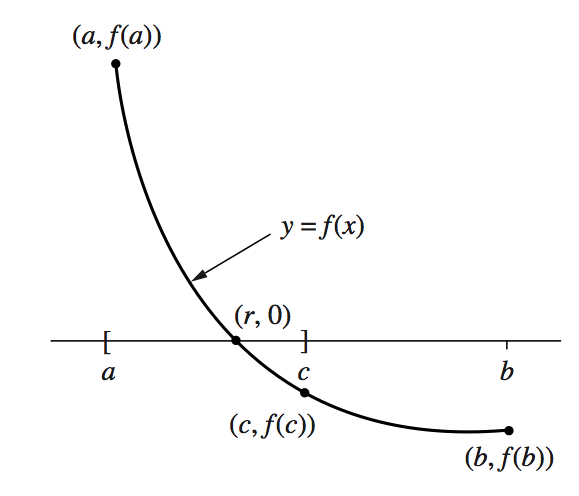
\includegraphics[width=50mm]{chap-1/fig_2-6.png}
\caption{If $f(a)$ and $f(c)$ have opposeite signs, then squeeze from the right.}
\end{center}
\end{figure}
\end{column}
\begin{column}{0.5\textwidth}
\begin{figure}
\begin{center}
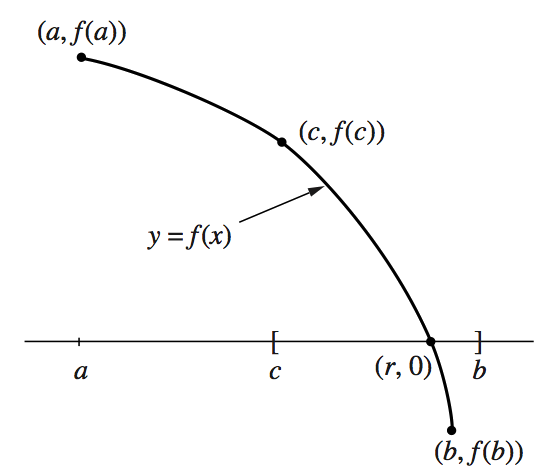
\includegraphics[width=50mm]{chap-1/fig_2-6_2.png}
\caption{If $f(c)$ and $f(b)$ have opposite signs, then squeeze from the left.}
\end{center}
\end{figure}
\end{column}
\end{columns}
}

\frame{
\begin{block}{Theorem (Bisection Theorem).}
Assume that $f \in C[a, b]$ and that there exists a number $r \in [a,b]$ such that $f(r) = 0$. 
If $f(a)$ and $f(b)$ have opposite signs, and $\{c_n\}_{n=0}^{\infty}$ represents the sequence of midpoints generated by the bisection process, then
\begin{equation*}
\left| r-c_n \right| \le \frac{b-a}{2^{n+1}} \ \ \ for n=0, 1, \ldots, 
\end{equation*}
and therefore the sequence $\{c_n\}_{n=0}^{\infty}$ converges to the zero $x = r$;
that is,
\begin{equation*}
\lim_{n \rightarrow \infty} c_n = r. 
\end{equation*}
\end{block}
}

\frame{
\frametitle{Proof of Theorem.}
Since both the zero $r$ and the midpoint $c_n$ lie in the interval $[a_n , b_n ]$, the distance between $c_n$ and $r$ cannot be greater than half the width of this interval. 
Thus
\begin{equation*}
\left| r - c_n \right| \le \frac{b_n-a_n}{2} \ \ \ for \  all \ n.
\end{equation*}
Observe that the successive interval widths form the pattern
\begin{equation*}
\begin{array}{l}
b_1 - a_1 = \frac{b_0 - a_0}{2^1} \\
b_2 - a_2 =\frac{b_1-a_1}{2} = \frac{b_0 - a_0}{2^2}. \\
\end{array} 
\end{equation*}
}

\frame{
\begin{equation*}
\begin{array}{c}
b_n - a_n = \frac{b_0 - a_0}{2^{n+1}}. \\
\Downarrow \\
|r-c_n| \le \frac{b_0 - a_0}{2^{n+1}} \ \ \ for \ all \ n.
\end{array}
\end{equation*}
\begin{figure}
\begin{center}
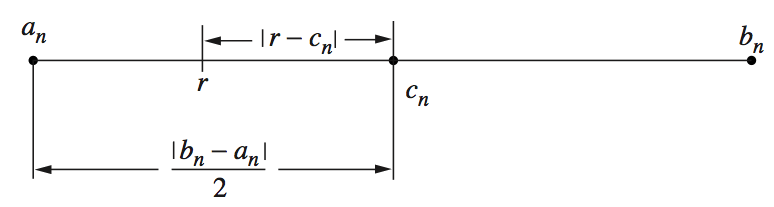
\includegraphics[width=100mm]{chap-1/fig_2-7.png}
\caption{The root $r$ and midpoint $c_n$ of $[a_n,b_n]$ for the bisection method.}
\end{center}
\end{figure}
}

\frame{
\begin{block}{Example.}
The function $h(x) = x \sin(x)$ occurs in the study of undamped forced oscillations. 
Find the value of $x$ that lies in the interval $[0, 2]$, where the function takes on the value $h(x) = 1$ (the function sin(x) is evaluated in radians).
\end{block}
We use the bisection method to find a zero of the function $f (x) = x \sin(x) - 1$. 
Starting with $a_0 = 0$ and $b_0 =2$, we compute
\begin{equation*} 
f (0) = -1.000000 \ \ \ and \ \ \ f (2) = 0.818595, 
\end{equation*}
so a root of $f(x) = 0$ lies in the interval $[0,2]$. 
At the midpoint $c_0 = 1$, we find that $f (1) = -0.158529$. 
Hence the function changes sign on $[c_0, b_0] = [1, 2]$.
}

\frame{
\begin{figure}
\begin{center}
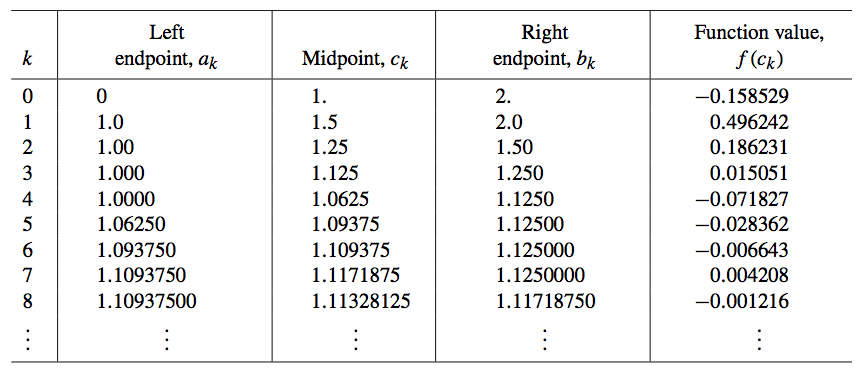
\includegraphics[width=90mm]{chap-1/tab_2-1.png}
\end{center}
\end{figure}
In this manner we obtain a sequence $\{c_k\}$ that converges to $r \approx 1.114157141$.
}

\frame{
\frametitle{Method of {\huge false position} or the {\huge regula false} method}
\framesubtitle{It was developed because the bisection method converges at a fairly slow speed.}
We assume that $f (a)$ and $f (b)$ have opposite signs. 
A better approximation is obtained if we find the point $(c, 0)$ where the secant line $L$ joining the points $(a, f (a))$ and $(b, f (b))$ crosses the x-axis. 
\begin{columns}
\begin{column}{0.5\textwidth}
\begin{figure}
\begin{center}
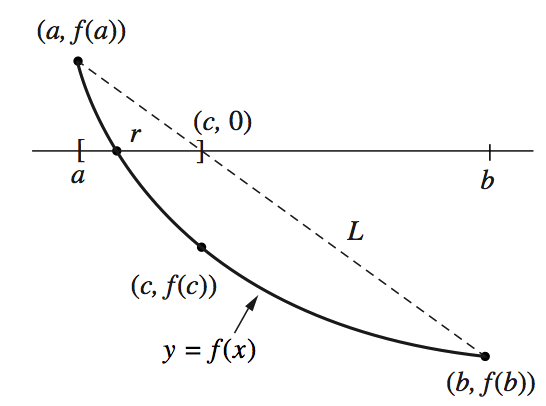
\includegraphics[width=45mm]{chap-1/fig_2-8.png}
\caption{If $f(a)$ and $f(c)$ have opposeite signs, then squeeze from the right.}
\end{center}
\end{figure}
\end{column}
\begin{column}{0.5\textwidth}
\begin{figure}
\begin{center}
\includegraphics[width=45mm]{chap-1/fig_2-8_2.png}
\caption{If $f(c)$ and $f(b)$ have opposite signs, then squeeze from the left.}
\end{center}
\end{figure}
\end{column}
\end{columns}
}

\frame{
To find the value $c$, we write down two versions of the slope m of the line $L$:
\begin{equation*}
m = \frac{f(b)-f(a)}{b-a}
\end{equation*}
where the points $(a, f (a))$ and $(b, f (b))$ are used, and 
\begin{equation*}
m = \frac{0- f(b)}{c-b}
\end{equation*}
the points $(c, 0)$ and $(b, f (b))$ are used.
}

\frame{
We can get :
\begin{equation*}
\frac{f(b)- f(a)}{b-a} = \frac{0- f(b)}{c-b}
\end{equation*}
which is easily solved for $c$ to get 
\begin{equation*}
c = b- \frac{f(b)(b-a)}{f(b)- f(a)}
\end{equation*}
\begin{block}{The three possibilities are the same as before:}
\begin{itemize}
\item If $f (a)$ and $f (c)$ have opposite signs, a zero lies in $[a, c]$. 	
\item If $f (c)$ and $f (b)$ have opposite signs, a zero lies in $[c, b]$.
\item If $f(c)=0$,then the zero is c.
\end{itemize}
\end{block}
}


\frame{
\frametitle{Exercises and Program}
\begin{block}{}
Find an approximation for the interest rate $I$ that will yield the total annuity value $A$ if $240$ monthly payments $P$ are made.  \\
Use the two starting values for $I$ and compute the next three approximations using the bisection method.
\begin{itemize}
\item $P = \$275$, $A = \$250,000$, $I_0 = 0.11$, $I_1 = 0.12$
\item $P = \$325$, $A = \$400,000$, $I_0 = 0.13$, $I_1 = 0.14$
\end{itemize}
\end{block}
}



\subsection{Iteration for Solving $x = g(x)$}

\frame{
\begin{block}{Iteration}
As the name suggests, a process is repeated until an answer is achieved.
\end{block}
\begin{itemize}
\item A rule of function $g(x)$
\item Starting value $p_0$
\item a sequence of values $\left\{ p_k \right\}$ is obtained using the iterative rule $p_{k+1} = g( p_k )$. 
\end{itemize}
\begin{block}{The sequence has the pattern}
\begin{table}[!h]
\begin{tabular}{l l l}
$p_0$ & & (starting value) \\
$p_1$ & = $g(p_0)$ & \\
$p_2$ & = $g(p_1)$ & \\
& $\vdots$ & \\
$p_k$ & = $g(p_{k-1})$ & \\
$p_{k+1}$ & = $g(p_k)$ & \\
& $\vdots$ & 
\end{tabular}
\end{table}
\end{block}
}

\frame{
\begin{block}{Example.}	
The iterative rule $p_0 = 1$ and $p_{k+1} = 1.001 p_k$ for $k = 0, 1, \ldots$ produces a divergent sequence. 
\end{block}
The first $100$ terms look as follows:
\begin{equation*}
\begin{array}{l l l l}
p_1 & =1.001p_0 & = (1.001)(1.000000) & = 1.001000, \\ 
p_2 & =1.001p_1 & = (1.001)(1.001000) & = 1.002001, \\
p_3 & =1.001p_2 & = (1.001)(1.002001) & = 1.003003, \\
\vdots & & \vdots & \vdots	\\ 
p_{100} & = 1.001 p_{99} & = (1.001)(1.104012) & = 1.105116.
\end{array}
\end{equation*}
The process can be continued indefinitely, and it is easily shown that $\lim_{n \rightarrow \infty} p_n = +\infty$.
}

\frame{
\begin{block}{Problems need to solve!}
\begin{itemize}
\item {\Large What can we learn from an unending sequence of numbers? }
\vspace{0.5cm}
\item {\Large If the numbers tend to a limit, we feel that something has been achieved. But what if the numbers diverge(发散) or are periodic(周期的)? }
\end{itemize}
\end{block}
}


\frame{
\frametitle{Finding Fixed Points}
\begin{block}{Definition .}
A {\Large fixed point} of a function $g(x)$ is a real number $P$ such that $P =g(P)$.\\
Geometrically, the fixed points of a function $y = g(x)$ are the points of intersection of $y = g(x)$ and $y = x$.
\end{block}
\vspace{0.5cm}
\begin{block}{Definition .}
The iteration $p_{n+1} = g(p_n)$ for $n = 0, 1, \ldots $ is called {\Large fixed-point iteration}.
\end{block}
}

\frame{
\begin{block}{Theorem .}
Assume that $g$ is a {\Large continuous function} and that $\{p_n\}_{n=0}^{\infty}$ is a sequence generated by fixed-point iteration.  \\
\vspace{0.5cm}
if $\lim_{n \rightarrow \infty} p_n = P$, then $P$ is a fixed point of $g(x)$.
\end{block}
\begin{block}{Proof.}	
If $lim_{n \rightarrow \infty} p_n = P$, then $lim_{n \rightarrow \infty} p_{n+1} = P$. It follows from this result, the
continuity of $g$, and the relation $p_{n+1} = g ( p_n )$ that
\begin{equation*}
g(P) = g \left( \lim_{n \rightarrow \infty} p_n \right) = \lim_{n \rightarrow \infty}  g(p_n)= \lim_{n \rightarrow \infty} p_{n+1} = P.
\end{equation*}
Therefore, $P$ is a {\Large fixed point} of $g(x)$.
\end{block}
}

\frame{
\frametitle{Example .}
\begin{block}{}
Consider the convergent iteration  \\
$p_0 =0.5$ and $p_{k+1} =e^{-p_k}$ for $k = 0, 1, \ldots$
\end{block}
\pause
The first $10$ terms are obtained by the calculations
\begin{table}[!h]
\begin{tabular}{l}
$p_1 = e^{-0.500000} = 0.606531$\\
$p_2 = e^{-0.606531} = 0.545239$ \\
$p_3 = e^{-0.545239} = 0.579703$\\
$\vdots$ \\
$p_9 = e^{-0.566409} = 0.567560$ \\
$p_{10} = e^{-0.567560} = 0.566907$ \\ 
\end{tabular}
\end{table}
The sequence is {\Large converging}, and further calculations reveal that
\begin{equation*}
lim_{n \rightarrow \infty} p_n = 0.567143....
\end{equation*}
Thus we have found an approximation for the fixed point of the function $y = e^{-x}$ .
}

\frame{
\begin{block}{Theorem.}	
Assume that $g \in C[a, b]$.
\begin{itemize}
\item If the range of the mapping $y = g(x)$ satisfies $y \in [a,b]$ for all $x \in [a,b]$, then $g$ has a fixed point in $[a, b]$.
\item Furthermore, suppose that $g′(x)$ is defined over $(a,b)$ and that apositive constant $K < 1$ exists with $|g′(x)| \le K < 1$ for all $x \in (a,b)$; then $g$ has a unique fixed point $P$ in $[a, b]$.
\end{itemize}
\end{block}
}

\frame{
\frametitle{Proof of Theorem.}
If $g(a) = a$ or $g(b) = b$, the assertion is true.  \\
Otherwise, the values of $g(a)$ and $g(b)$ must satisfy $g(a) \in (a, b]$ and $g(b) \in [a, b)$.  \\
The function $f (x) ≡ x - g(x)$ has the property that
\begin{equation*}
f (a) = a - g(a) < 0
\end{equation*}	
and
\begin{equation*}
f (b) = b - g(b) > 0.
\end{equation*}
Now apply the intermediate value theorem, to $f (x)$, with the constant $L = 0$, and conclude that there exists a number $P$ with $P \in (a,b)$ so that $f(P) = 0$. Therefore, $P = g(P)$ and $P$ is the desired fixed point of $g(x)$.
}

\frame{
\frametitle{Proof of Theorem (continued)}
By way of contradiction, let us make the additional assumption that there exist two fixed points $P_1$ and $P_2$. 
Apply  the mean value theorem, and conclude that there exists a number $d \in (a, b)$ so that
\begin{equation*}
g′(d)= \frac{g(P_2)-g(P_1)}{P2 - P1}. 
\end{equation*}
Use the facts that $g(P_1) = P_1$ and $g(P_2) = P_2$ to simplify the right side of the equation  and obtain
\begin{equation*}
g′(d) = \frac{P_2 - P_1}{P_2 - P_1} = 1. 
\end{equation*}
But this contradicts the hypothesis in above equation that $|g′(x)| < 1$ over $(a,b)$, so it is not possible for two fixed points to exist. Therefore, $g(x)$ has a unique fixed point $P$ in $[a, b]$ under the conditions given in above equation.
}

\frame{
\begin{block}{Theorem  (Fixed-Point Theorem).}
Assume that 
\begin{itemize}
\item (i) $g, g′ \in C[a, b]$, 
\item (ii) $K$ is a positive constant, 
\item (iii) $p_0 \in (a, b)$, 
\item (iv) $g(x) \in [a, b]$ for all $x \in [a, b]$.
\end{itemize}
\vspace{0.5cm}
\begin{itemize}
\item If $|g′(x)| \le K < 1$ for all $x \in [a,b]$, then the iteration $p_n = g(p_{n-1})$ will converge to the unique fixed point $P \in [a, b]$. 
$\rightarrow$
In this case, $P$ is said to be an attractive fixed point.
\item If $|g′(x)| > 1$ for all $x \in [a,b]$, then the iteration $p_n = g(p_{n-1})$ will not converge to $P$ . 
$\rightarrow$
In this case, $P$ is said to be a repelling fixed point and the iteration exhibits local divergence.
\end{itemize}
\end{block}
}

\frame{
\begin{block}{Corollary\footnote{推论} 1.1.}
Assume that $g$ satisfies the hypothesis given in of Theorem 1.3. 
Bounds for the error involved when using pn to approximate $P$ are given by
\begin{equation*}
\left| P-p_n \right| \le K^n \left| P-p_0 \right| \ \ \ for \ all \ n\ge 1 
\end{equation*}
and
\begin{equation*}
\left| P-p_n \right| \le \frac{K^n \left| p_1-p_0 \right|}{1-K} \ \ \ for \ all \ n \ge 1. 
\end{equation*}
\end{block}
}

\frame{
\frametitle{Graphical Interpretation of Fixed-Point Iteration}
\begin{columns}
\begin{column}{0.5\textwidth}
\begin{figure}
\begin{center}
\includegraphics[width=60mm]{chap-1/fig_2-4.png}
\caption{Monotone convergence (单调收敛) when $0 < g`(P) < 1$}
\end{center}
\end{figure}
\end{column}
\begin{column}{0.5\textwidth}
\begin{figure}
\begin{center}
\includegraphics[width=60mm]{chap-1/fig_2-4_2.png}
\caption{Oscillating converagence (振荡收敛) when $-1 < g`(P) < 0$}
\end{center}
\end{figure}
\end{column}
\end{columns}
}

\frame{
\begin{block}{}
if $|g`(P)| > 1$, then the iteration $p_{n+1} = g(p_n)$ produces a sequence that diverages away from $P$.
\end{block}
\begin{columns}
\begin{column}{0.5\textwidth}
\begin{figure}
\begin{center}
\includegraphics[width=60mm]{chap-1/fig_2-5.png}
\caption{Monotone divergence when $1 < g`(P)$}
\end{center}
\end{figure}
\end{column}
\begin{column}{0.5\textwidth}
\begin{figure}
\begin{center}
\includegraphics[width=60mm]{chap-1/fig_2-5_2.png}
\caption{Divergent Oscillating when $g`(P) < -1$}
\end{center}
\end{figure}
\end{column}
\end{columns}
}



\frame{
\frametitle{Exercises and Program}
\begin{block}{Determine rigorously if each function has a unique fixed point on the given interval.}
\begin{itemize}
\item $g(x)=1-x^2/4$ on $[0,1]$ 
\item $g(x)=2^{-x}$ on $[0,1]$
\item $g(x) = 1/x$ on $[0.5, 5.2]$
\end{itemize}
\end{block}
}





\subsection{Newton-Raphson and Secant Methods}

\frame{
\frametitle{Slope Methods for Finding Roots}
\begin{block}{}
If $f (x)$, $f'(x)$, and $f''(x)$ are continuous near a root $p$, then this extra information regarding the nature of $f (x)$ can be used to develop algorithms that will produce sequences $\{ p_k \}$ that converge faster to $p$ than either the bisection or false position method.
\end{block}

{\Large The Newton-Raphson (or simply Newton’s) method is one of the most useful and best known algorithms that relies on the continuity of $f'(x)$ and $f''(x)$. }
}

\frame{
Assume that the initial approximation $p_0$ is near the root p.  \\
\begin{itemize}
\item Then the graph of $y = f (x)$ intersects the x-axis at the point $(p, 0)$, and the point $(p_0, f(p_0))$ lies on the curve near the point $(p, 0)$. 
\item Define $p_1$ to be the point of intersection of the x-axis and the line tangent to the curve at the point $(p_0, f(p_0))$.
\end{itemize}
\begin{figure}
\begin{center}
\includegraphics[width=60mm]{chap-1/fig_2-13.png}
\end{center}
\end{figure}
\begin{block}{}
It is shown that $p_1$ will be closer to $p$ than $p_0$ in this case.
\end{block}
}


\frame{
An equation relating $p_1$ and $p_0$ can be found if we write down two versions for the slope of the tangent line $L$:
\begin{equation*}
m = \frac{0 - f(p_0)}{p_1-p_0} 
\end{equation*}
which is the slope of the line through $(p_1, 0)$ and $(p_0, f(p_0))$,  and
\begin{equation*}
m =  f'(p_0) 
\end{equation*}
which is the slope at the point $(p_0, f(p_0))$. \\
\begin{center}
$\Downarrow $
\end{center}
\begin{equation*}
p_1 =  p_0 - \frac{f(p_0)}{f'(p_0)} 
\end{equation*}
\begin{block}{}
This process can be repeated to obtain a sequence $\{ p_k \}$ that converges to $p$.
\end{block}
}

\frame{
\begin{block}{Theorem (Newton-Raphson Theorem)}
Assume that $f \in C^2[a, b]$ and there exists a number $p \in [a, b]$, where $f(p) = 0$. 
If $f'(p) \neq 0$, then there exists a $\delta > 0$ such that the sequence $\{p_k\}^{\infty}_{k=0}$ defined by the iteration
\begin{equation*}
p_k = g(p_{k-1}) =  p_{k-1} - \frac{ f(p_{k-1}) }{ f'(p_{k-1}) }  \ \ \ for \ \ \ k=1,2,\ldots
\end{equation*}
will converge to $p$ for any initial approximation $p_0 \in [p - \delta, p + \delta]$.
\end{block}
\begin{block}{Remark}
The function $g(x)$ defined by the formula
\begin{equation*}
 g(x) = x - \frac{ f(x) }{ f'(x) } 
\end{equation*}
is called the {\Large Newton-Raphson iteration function}.
\end{block}
}

\frame{
\frametitle{Proof of Theorem}
The Taylor polynomial of degree $n = 1$ and its remainder term:
\begin{equation*}
 f(x) = f(p_0)  + f'(p_0) (x - p_0) + \frac{ f''(c) (p-P_0)^2 }{ 2! } 
\end{equation*}
where $c$ lies somewhere between $p_0$ and $x$.
\begin{center}
$\Downarrow $
\end{center}
Substituting $x = p$ into the equation  and using the fact that $f (p) = 0$ produces
\begin{equation*}
 0 = f(p_0)  + f'(p_0) (x - p_0) + \frac{ f''(c) (p-P_0)^2 }{ 2! } 
\end{equation*}
}

\frame{
\frametitle{Proof of Theorem  (continued)}
If $p_0$ is close enough to $p$, the last term on the right side of above function\footnote{ Taylor polynomial} will be small compared to the sum of the first two terms.
\begin{center}
$\Downarrow $
\end{center}
Hence it can be neglected and we can use the approximation
\begin{equation*}
 0 \approx f(p_0)  + f'(p_0) (x - p_0)  
\end{equation*}
\begin{center}
$\Downarrow $
\end{center}
Solving for $p$ in the equation, we get $p \approx p_0 - f (p_0) \/ f'(p0)$.
\begin{center}
$\Downarrow $
\end{center}
This is used to define the next approximation p1 to the root
\begin{equation*}
p_1 \approx p_0  - \frac{f(p_0)}{ f' (p_0)}
\end{equation*}
}

\frame{
\frametitle{Proof of Theorem (continued)}
\begin{center}
$\Downarrow $
\end{center}
When $p_{k-1}$ is used in place of $p_0$ in equation, the general rule is established.
\begin{center}
$\Downarrow $
\end{center}
However, to fully comprehend what is happening, we need to consider the fixed-point iteration function and apply Theorem 1.2 in our situation.
The key is in the analysis of $g'(x)$:
\begin{equation*}
g'(x)   = 1 - \frac{f'(x)f'(x) - f(x)f''(x)}{(f'(x))^2 } =   \frac{f(x)f''(x)}{(f'(x))^2 }
\end{equation*}
}

\frame{
\frametitle{Proof of Theorem (continued)}
Since $g'(p) = 0$ and $g'(x)$ is continuous,  
it is possible to find a $\delta > 0$ so that the hypothesis $| g'(x) | < 1$ is satisfied on $( p - \delta, p + \delta )$.
\begin{center}
$\Downarrow $
\end{center}
Therefore, a sufficient condition for $p_0$ to initialize a convergent sequence $\{ p_k \}^{\infty}_{k=0}$, which converges to a root of $f (x) = 0$, is that $p_0 \in (p - \delta, p + \delta)$ and that $\delta$ be chosen so that
\begin{equation*}
 \frac{| f(x)f''(x)| }{| (f'(x))|^2 } < 1 \ \ \ for \ \ all \ \ x \in  (p - \delta, p + \delta)
\end{equation*}
}

\frame{
\begin{block}{Corollary  (Newton’s Iteration for Finding Square Roots).}
Assume that $A > 0$ is a real number and let $p_0 > 0$ be an initial approximation to $\sqrt{A}$.
Define the sequence $\{ p_k \}^{\infty}_{k =0}$ using the recursive rule
\begin{equation*}
p_k = \frac{p_{k-1}+\frac{A}{p_{k-1}}}{2}
\end{equation*}
for $k =  1, 2, \ldots$
Then the sequence $\{ p_k \}^{\infty}_{k =0}$ converges to $\sqrt{A}$; that is, $\lim_{n \rightarrow \infty} p_k = \sqrt{A}$.
\end{block}
}

\frame{
\frametitle{Proof of Corollary (Newton’s Iteration for Finding Square Roots).}
Start with the function $f (x) = x^2 - A$, and notice that the roots of the equation $x^2 - A = 0$ are $\pm \sqrt{A}$.
\begin{center}
$\Downarrow $
\end{center}
write down the {\Large Newton-Raphson iteration formula}
\begin{equation*}
g(x) = x - \frac{f(x)}{f'(x)} = x - \frac{x^2 - A}{2x}
\end{equation*}
\begin{center}
$\Downarrow $
\end{center}
This formula can be simplified to obtain
\begin{equation*}
g(x) = x - \frac{x+\frac{A}{x}}{2} 
\end{equation*}
}

\frame{
\frametitle{Division-by-Zero Error}
\begin{itemize}
\item One obvious pitfall of the Newton-Raphson method is the possibility of division by zero in the formula, which would occur if $f'(p_{k-1}) = 0$.
\item It is quite possible that $f (p_{k-1})$ is sufficiently close to zero and that $p_{k-1}$ is an acceptable approximation to the root. 
\end{itemize}
\begin{block}{}
We now investigate this situation and will uncover an interesting fact, that is, how fast the iteration converges.
\end{block}
}

\frame{
\begin{block}{Definition.}
Assume that $f (x)$ and its derivatives $f'(x), \ldots, f^{(M)}(x)$ are defined and continuous on an interval about $x = p$. 
We say that $f (x) = 0$ has a {\Large root of order} $M$ at x = p if and only if
\begin{center}
$f(p) = 0$, $f'(p)=0$, $\ldots$, $f^{(M-1)}(p)=0$, and $f^{(M)}(p) \ne 0$
\end{center}
\end{block}
A root of order $M = 1$ is often called a {\Large simple root}, and if $M > 1$, it is called a {\Large multiple root}. 
A root of order $M = 2$ is sometimes called a {\Large double root}, and so on.
}

\frame{
\begin{block}{Lemma(引理).}
If the equation $f (x) = 0$ has a root of order $M$ at $x = p$, then there exists a continuous function $h(x)$ so that $f (x)$ can be expressed as the product
\begin{equation*}
f(x) = (x -p)^M h(x), \ \ \ where \ \ h(p) \ne 0
\end{equation*}
\end{block}
Proof :\\
By the Taylor formula, we can expand $f(x)$ about $x=p$ to get
\begin{equation*}
f(x) = (x-p)^M\frac{f^{(M)}(c(x))}{M!}
\end{equation*}
where $c(x)$ is between $p$ and x.
$h(x)$ is continuous on an interval about $x =p$, and 
\begin{equation*}
h(p) = \lim_{x \rightarrow \infty} \frac{f^{(M)}(c(x))}{M!} = \frac{f^{(M)}(p)}{M!} \ne 0
\end{equation*}
}

\frame{
\frametitle{Speed of Convergence}
\begin{itemize}
\item If $p$ is a simple root of $f (x) = 0$, {\Large Newton’s method} will converge rapidly, and the number of accurate decimal places (roughly) doubles with each iteration. 
\item On the other hand, if $p$ is a multiple root, the error in each successive approximation is a fraction of the previous error. 
\end{itemize}
\begin{block}{}
To make this precise, we define the {\Large order of convergence}. 
This is a measure of how rapidly a sequence converges.
\end{block}
}

\frame{
\begin{block}{Definition}
Assume that $\{p_n\}^{\infty}_{n=0}$ converges to $p$ and set $E_n = p - p_n$ for $n \ge 0$.
If two positive constants $A \ne 0$ and $R>0$ exist, and
\begin{equation*}
\lim_{n \rightarrow \infty} \frac{|p-p_{n+1}|}{|p-p_n|^R} = \lim_{n \rightarrow \infty} \frac{E_{n+1}}{|E_n|^R} = A,
\end{equation*}
then the sequence is said to converge to $p$ with {\Large order of convergence} $R$. 
The number $A$ is called the {\Large asymptotic error constant}. 
The cases $R = 1, 2$ are given special consideration:
\begin{itemize}
\item If $R = 1$, the convergence of $\{p_n\}^{\infty}_{n=0}$ is called {\Large linear}.
\item If $R = 2$, the convergence of $\{p_n\}^{\infty}_{n=0}$ is called {\Large quadratic}.
\end{itemize}
\end{block}
If $R$ is large, the sequence $\{ p_n \}$ converges rapidly to $p$; 
for large values of $n$ we have the approximation $|E_{n+1}| \approx A|E_n|^R$.
}

\frame{
\begin{block}{Theorem (Convergence Rate for Newton-Raphson Iteration).}
Assume that Newton-Raphson iteration produces a sequence $\{ p_n \}^{\infty}_{n = 0}$ that converges to the root $p$ of the function $f (x)$.
\begin{itemize}
\item If $p$ is a simple root, convergence is quadratic and
\begin{equation*}
|E_{n+1}| \approx \frac{|f''(p)|}{2|f'(p)|}|E_n|^2 \ \ \ for \ \ n \ \ sufficiently \ \ large.
\end{equation*}
\item If $p$ is a multiple root of order $M$, convergence is linear and
\begin{equation*}
|E_{n+1}| \approx \frac{M-1}{M}|E_n| \ \ \ for \ \ n \ \ sufficiently \ \ large.
\end{equation*}
\end{itemize}
\end{block}
}

\frame{
\frametitle{Secant Method(割线法)}
\begin{itemize}
\item The Newton-Raphson algorithm requires the evaluation of two functions per iteration, $f(p_{k-1})$ and $f'(p_{k-1})$. 
\item Traditionally, the calculation of derivatives of elementary functions could involve considerable effort. 
\item But with modern computer algebra software packages, this has become less of an issue. 
\item Still many functions have nonelementary forms (integrals, sums, etc.), and it is desirable to have a method that converges almost as fast as Newton’s method yet involves only evaluations of $f(x)$ and not of $f'(x)$.
\end{itemize}
\begin{block}{}
The secant method will require only one evaluation of $f (x)$ per step and at a simple root has an order of convergence $R \approx 1.618033989$. 
It is almost as fast as Newton’s method, which has order $2$.
\end{block}
}

\frame{
\begin{itemize}
\item Two initial points $(p_0, f (p_0))$ and $(p_1, f (p_1))$ near the point $(p, 0)$ are needed;
\item Define $p_2$ to be the abscissa\footnote{横坐标} of of the point of intersection of the line through these two points and the x-axis;
\item The equation relating $p_2$, $p_1$, and $p_0$ is found by considering the slope
\begin{equation*}
m = \frac{f(p_1)-f(p_0)}{p_1-p_0} \ \ \ and \ \ \ m = \frac{0-f(p_1)}{p_2-p_1}
\end{equation*}
\end{itemize}
\begin{figure}
\begin{center}
\includegraphics[width=45mm]{chap-1/fig_2-16.png}
\caption{The geometric construction of $p_2$ for the secant method.}
\end{center}
\end{figure}
}

\frame{
The values of $m$ in above equation are the slope of the secant line through the first two approximations and the slope of the line through $(p_1, f (p_1))$ and $(p_2, 0)$, respectively.
\begin{center}
$\Downarrow $
\end{center}
solve for $p_2 = g(p_1, p_0)$ and get
\begin{equation*}
p_2 = g(p_1,p_0)  = p_1 - {f(p_1)(p_1-p_0)}{f(p_1)-f(p_0)}
\end{equation*}
\begin{center}
$\Downarrow $
\end{center}
The general term is given by the two-point iteration formula
\begin{equation*}
p_{k+1} = g(p_k,p_{k-1})  = p_k - {f(p_k)(p_k-p_{k-1})}{f(p_k)-f(p_{k-1})}
\end{equation*}
}

\frame{
\frametitle{Accelerated Convergence}
\begin{itemize}
\item We could hope that there are root-finding techniques that converge faster than linearly when $p$ is a root of order $M$. 
\item Our final result shows that a modification can be made to Newton’s method so that convergence becomes quadratic at a multiple root.
\end{itemize}
}

\frame{
\begin{block}{Theorem  (Acceleration of Newton-Raphson Iteration).}
Suppose that the Newton-Raphson algorithm produces a sequence that converges linearly to the root $x = p$ of order $M > 1$. 
Then the Newton-Raphson iteration formula
\begin{equation*}
p_k = p_{k-1} - \frac{M f(p_{k-1})}{f'(p_{k-1})}
\end{equation*}
will produce a sequence $\{ p_k \}^{\infty}_{k = 0}$ that converges quadratically to $p$.
\end{block}
}






%\setcounter{section}{1}



%\section{Solution of Linear Systems $AX = B$}
\section{解线性代数方程组的直接法}


%


\frame{
Three planes form the boundary of a solid in the first octant\footnote{成$45$度视角的位置,八分圆}, which is shown in the following figure. 
\begin{figure}
\begin{center}
\includegraphics[width=45mm]{chap-2/fig_3-1.png}
%\caption{The portion of a sphere of radius $r$ that is to be submerged to a depth $d$}
\end{center}
\end{figure}
Suppose that the equations for these planes are
\begin{equation*}
\begin{array}{r r r r}
5x + & y + & z = & 5 \\
x + & 4y + & z = & 4 \\
x + & y + & 3z = & 3
\end{array}
\end{equation*}
}

\frame{
\begin{block}{}
{\Large What are the coordinates of the point of intersection of the three planes? }
\end{block}
\begin{center}
$\Downarrow$
\end{center}
{\Large Gaussian elimination} can be used to find the solution of the linear system
\begin{center}
$\Downarrow$
\end{center}
\begin{equation*}
\begin{array}{ l l }
x & = 0.76 \\
y & = 0.68 \\
z & = 0.52
\end{array}
\end{equation*}
}





%\subsection{Introduction to Vectors and Matrices}



\frame{
\frametitle{Vectors}
A real $N$-dimensional vector $X$ is an ordered set of $N$ real numbers and is usually written in the coordinate form
\begin{equation*}
 X = \left( x_1, x_2, \ldots, x_N \right).
\end{equation*}
Here :
\begin{itemize}
\item The numbers $x_1$, $x_2$, $\ldots$, and $x_N$ are called the {\Large components} or {\Large coordinates} of $X$.
\item The set consisting of all $N$-dimensional vectors is called {\Large $N$-dimensional space}.
\item When a vector is used to denote a point or position in space, it is called a {\Large position vector}. 
\item When it is used to denote a movement between two points in space, it is called a {\Large displacement vector}.
\end{itemize}
}

\frame{
Let another vector be $Y = (y_1, y_2, \ldots, y_N )$. 
\begin{itemize}
\item The two vectors $X$ and $Y$ are said to be equal if and only if each corresponding coordinate is the same; 
that is, $X = Y$ if and only if $x_j = y_j$ for $j = 1, 2, \ldots, N$. 
\item The sum of the vectors $X$ and $Y$ is computed component by component, using the definition
\begin{equation*}
X + Y = \left( x_1+y_1, x_2+y_2, \cdots, x_N+y_N\right)
\end{equation*}
\item The negative of the vector X is obtained by replacing each coordinate with its
negative:
\begin{equation*}
- X = \left( -x_1, -x_2, \cdots, -x_N\right)
\end{equation*}
\item The difference $Y - X$ is formed by taking the difference in each coordinate:
\begin{equation*}
 Y - X = \left( y_1-x_1, y_2-x_2, \cdots, y_N-x_N\right)
\end{equation*}
\end{itemize}
}

\frame{
\begin{itemize}
\item Vectors in $N$-dimensional space obey the algebraic property
\begin{equation*}
Y - X = Y + (-X)
\end{equation*}
\item If $c$ is a real number (scalar), we define {\Large scalar multiplication} $cX$ as follows:
\begin{equation*}
c X = \left( c x_1, c x_2 \cdots, c x_N\right)
\end{equation*}
\item If $c$ and $d$ are scalars, then the weighted sum $cX +dY$ is called a {\Large linear combination} of $X$ and $Y$, and we write
\begin{equation*}
c X + d Y = \left( c x_1 + d y_1, c x_2 + d y_2 \cdots, c x_N + d y_N\right)
\end{equation*}
\end{itemize}
}

\frame{
\begin{itemize}
\item The {\Large dot product} of the two vectors $X$ and $Y$ is a scalar quantity (real number) defined by the equation
\begin{equation*}
 X \cdot Y = \left(  x_1  y_1 + x_2 y_2 + \cdots  x_N y_N\right)
\end{equation*}
\item The {\Large norm} (or {\Large length})\footnote{referred as the {\Large Euclidean norm} (or {\Large length} ) of the vector $X$} of the vector $X$ is defined by
\begin{equation*}
 || X || = \left(  x_1^2 + x_2^2  + \cdots + x_N^2 \right)^{1 \slash 2}
\end{equation*}
\end{itemize}

\begin{block}{}
\begin{equation*}
\begin{array}{r}
 || c X || = \left( c^2 x_1^2 + c^2 x_2^2  + \cdots + c^2 x_N^2 \right)^{1 \slash 2} \\
= |c |  \left(  x_1^2 +  x_2^2  + \cdots +  x_N^2 \right)^{1 \slash 2}  = |c| \  ||X||
\end{array}
\end{equation*}
\begin{equation*}
|| X ||^2 = x_1^2 + x_2^2 + \cdots + x_N^2 = X \cdot X
\end{equation*}
\begin{equation*}
|| Y - X || = \left( (y_1 - x_1)^2 + (y_2 - x_2)^2 + \cdots + (y_N - x_N)^2 \right)^{1 \slash 2}
\end{equation*}
\end{block}
}

\frame{
\frametitle{Vector Algebra}
Suppose that $X$, $Y$, and $Z$ are $N$-dimensional vectors and $a$ and $b$ are scalars (real numbers). 
The following properties of vector addition and scalar multiplication hold:
\begin{itemize}
\item commutative property : $Y + X = X + Y$
\item additive identity : $0 + X = X + 0$
\item additive inverse : $X - X = X + (-X) = 0$
\item associative property : $(X + Y) + Z = X + (Y + Z)$
\item distributive property for scalars : $(a + b)X = aX + bX$
\item distributive property for vectors : $a(X + Y) = aX + aY$
\item associative property for scalars : $a(bX) = (ab)X$
\end{itemize}
}

\frame{
\frametitle{Matrices and Two-Dimensional Arrays}
\begin{itemize}
\item A matrix is a rectangular array of numbers that is arranged systematically in rows and columns. 
\item A matrix having $M$ rows and $N$ columns is called an $M \times N$ \footnote{read “M by N”} matrix. 
\item The capital letter A denotes a matrix, and the lowercase subscripted letter $a_{i, j}$ denotes one of the numbers forming the matrix. 
\end{itemize}
}

\frame{
We write
\begin{equation*}
A = [a_{i,j}]_{M \times N} \ \ \ for 1 \le i \le M, \ \  1 \le j \le N,
\end{equation*}
where $a_{i,j}$ is the number in location $(i, j)$ \footnote{i.e., stored in the ith row and j th column
of the matrix}. 
We refer to $a_{i, j}$ as the element in location $(i, j )$.
In expanded form we write
\begin{equation*}
row \ \ i \rightarrow
\left[
\begin{array}{ c c c c c c}
a_{1,1} & a_{1,2} & \cdots &a_{1,j} & \cdots & a_{1,N} \\
a_{2,1} & a_{2,2} & \cdots &a_{2,j} & \cdots & a_{2,N} \\
\vdots & \vdots &  &\vdots &  & a_{1,N} \\
a_{i,1} & a_{i,2} & \cdots &a_{i,j} & \cdots & a_{i,N} \\
\vdots & \vdots &         &\vdots &        & a_{1,N} \\
a_{N,1} & a_{N,2} & \cdots &a_{N,j} & \cdots & a_{N,N}
\end{array}
\right]
= A
\end{equation*}
\begin{equation*}
\begin{array}{c}
\uparrow \\
column \ \  j
\end{array}
\end{equation*}
}

\frame{
The rows of the $M \times N$ matrix $A$ are $N$-dimensional vectors:
\begin{equation*}
V_i = \left( a_{i1}, a_{i2}, \cdots , a_{i N} \right)  \ \ \ \  for \ \  i = 1, 2, \ldots, M.
\end{equation*}
The row vectors can also be viewed as $1 \times N$ matrices $V_i$.
\begin{equation*}
A = 
\left[
\begin{array}{c}
V_1 \\
V_2 \\
\vdots \\
V_i \\
\vdots \\
V_M
\end{array}
\right]
= \left[ V_1, V_2, \cdots, V_i, \cdots, V_M\right]^T
\end{equation*}
}

\frame{
Similarly, the columns of the $M \times N$ matrix $A$ are $M \times 1$ matrices:
\begin{equation*}
C_1 = 
\left[ 
\begin{array}{c}
a_{1,1} \\
a_{2,1} \\
\vdots \\
a_{i,1} \\
\vdots \\
a_{M,1}
\end{array}
\right],
\cdots,
C_j = 
\left[ 
\begin{array}{c}
a_{1,j} \\
a_{2,j} \\
\vdots \\
a_{i,j} \\
\vdots \\
a_{M,j}
\end{array}
\right],
\cdots,
C_N = 
\left[ 
\begin{array}{c}
a_{1,N} \\
a_{2,N} \\
\vdots \\
a_{i,N} \\
\vdots \\
a_{M,N}
\end{array}
\right]
\end{equation*}
In this case we could express $A$ as a $1\times N$ matrix consisting of the $M \times 1$ column matrices $C_j$ :
\begin{equation*}
A = \left[ C_1, C_2, \cdots, C_j, \cdots, C_N \right]
\end{equation*}
}

\frame{
Let $A = [a_{i,j} ]_{M \times N}$ and $B = [b_{i, j} ]_{M \times N}$ be two matrices of the same dimension.
\begin{itemize}
\item $A=B$  if and only if $a_{i, j} = b_{i, j}$ for $1 \le i \le M$, $1 \le j\le N$.
\item $A+B = \left[ a_{i, j} + b_{i, j} \right]_{M \times N}$ for $1 \le i \le M$, $1 \le j\le N$.
\item $-A = \left[ - a_{i,j} \right]_{M \times N}$  for $1 \le i \le M$, $1 \le j\le N$.
\item $A - B = \left[ a_{i, j} - b_{i, j} \right]_{M \times N}$ for $1 \le i \le M$, $1 \le j\le N$.
\item $cA = \left[ c a_{i,j} \right]_{M \times N}$  for $1 \le i \le M$, $1 \le j\le N$.
\item $pA + qB = \left[ p a_{i,j} + q b_{i,j} \right]_{M \times N}$ for $1 \le i \le M$, $1 \le j\le N$.
\end{itemize}
}

\frame{
\frametitle{Matrix Algebra}. 
Suppose that $A$, $B$, and $C$ are $M \times N$ matrices and $p$ and $q$ are scalars. 
The following properties of matrix addition and scalar multiplication hold:
\begin{itemize}
\item commutative property : $B + A = A + B$
\item additive identity : $0 + A = A + 0$
\item additive inverse : $A - A = A + (-A) = 0$
\item associative property : $(A + B) + C = A + (B + C)$
\item distributive property for scalars : $(p + q)A = pA + qA$
\item distributive property for vectors : $p(A + B) = pA + pB$
\item associative property for scalars : $p(qA) = (pq)A$
\end{itemize}

}



%\subsection{Upper-Triangular Linear Systems}


\frame{
\begin{itemize}
\item We will now develop the {\Large  back-substitution algorithm},  which is useful for solving a linear system of equations that has an upper-triangular coefficient matrix. 
\item This algorithm will be incorporated in the algorithm for solving a general linear system.
\end{itemize}
\vspace{3mm}
\begin{block}{Definition.}
\begin{itemize}
\item An  $N  \times N$ matrix  $A = [ a_{i , j} ]$ is called {\Large upper triangular} provided that the elements satisfy $ a_{i , j} = 0 $ whenever $ i > j $ . 
\item The $N \times N$ matrix  $A = [a_{i , j} ]$ is called {\Large lower triangular} provided that $a_{i,j} = 0$ whenever $i < j$.
\end{itemize}
\end{block}
}

\frame{
If $A$ is an upper-triangular matrix, then $A X = B$ is said to be an {\Large upper triangular system } of linear equations and has the form
\begin{equation*}
\begin{array}{ rl }
a_{1,1} x_1 + a_{1,2} x_2  + a_{1,3} x_3 + \cdots +  a_{1, N-1} x_{N-1} + a_{1, N} x_N & = b_1 \\
a_{2,2} x_2  + a_{2,3} x_3 + \cdots +  a_{2, N-1} x_{N-1} + a_{2, N} x_N & = b_2 \\
a_{3,3} x_3 + \cdots +  a_{3, N-1} x_{N-1} + a_{3, N} x_N & = b_3 \\
\vdots \ \ \ \ \ \ \ \ \ \ \ \ \ \ \ \ & \ \ \vdots \\
a_{N-1, N-1} x_{N-1} + a_{N-1, N} x_N & = b_{N-1} \\
a_{N,N} x_N & = b_N 
\end{array}
\end{equation*}
\begin{block}{Theorem (Back Substitution).}
Suppose that $A X = B$ is an upper-triangular system with the form given in above upper triangular system. 
If  $a_{k, k} \ne 0 \ \ \ for \ \ k = 1, 2, \ldots, N$,
then there exists a {\Large unique solution} to this upper triangular system.
\end{block}
}

\frame{
\begin{block}{Constructive Proof of Theorem:} 
\begin{itemize}
\item The last equation involves only $x_N$, so we solve it first:
\begin{equation*}
x_N = \frac{b_N}{a_{N,N}} 
\end{equation*}
\begin{center}
$\Downarrow$
\end{center}
\item Now $x_N$ is known and it can be used in the next-to-last equation:
\begin{equation*}
x_{N-1} = \frac{b_{N-1} - a_{N-1,N}x_N}{a_{N-1,N-1}}
\end{equation*}
\begin{center}
$\Downarrow$
\end{center}
\item Now $x_N$ and $x_{N-1}$ are used to find $x_{N-2}$ :
\begin{equation*}
x_{N-2} = \frac{b_{N-2} - a_{N-2,N-1}x_{N-1} - a_{N-2,N}x_N }{a_{N-2,N-2}}
\end{equation*}
\end{itemize}
\end{block}
}

\frame{
\begin{block}{Constructive Proof of Theorem (continued):} 
\vspace{5mm}
\begin{center}
$\Downarrow$
\end{center}
\begin{itemize}
\item Once the values $x_N, x_{N-1}, \ldots, x_{k+1}$ are known, the general step is
\begin{equation*}
x_k = \frac{b_k - \sum_{j = k + 1}^N  a_{k, j}x_j }{a_{k, k}}
\end{equation*}
\begin{center}
$\Downarrow$
\end{center}
\item The uniqueness of the solution is easy to see. 
\begin{itemize}
\item The $N$-th equation implies that $b_N  \slash a_{N, N}$ is the {\Large only possible value} of $x_N$ .
\item Then finite induction is used to establish that $x_{N-1}, x_{N-2}, \cdots , x_1$ are {\Large unique}.
\end{itemize}
\end{itemize}
\end{block}
}


\frame{
\frametitle{Example .}
Use {\Large back substitution} to solve the linear system
\begin{equation*}
\begin{array}{r l}
4x_1 - x_2 + 2x_3 + 3x_4 = & 20 \\
-2x_2 + 7x_3 - 4x_4 = & -7 \\
6x_3 + 5x_4 = & 4 \\
3x_4 = & 6.
\end{array}
\end{equation*}
\begin{center}
$\Downarrow$
\end{center}
Solving for $x_4$ in the last equation yields 
\begin{equation*}
x_4 = \frac{6}{3} = 2 
\end{equation*}
\begin{center}
$\Downarrow$
\end{center}
Using $x_4 = 2$ in the third equation, we obtain
\begin{equation*}
x_3 = \frac{4-5(2)}{6} = -1 
\end{equation*}
}

\frame{
\begin{center}
$\Downarrow$
\end{center}
Now $x_3 = -1$ and $x_4 = 2$ are used to find $x_2$ in the second equation:
\begin{equation*}
x_2 = \frac{-7 - 7 (-1) + 4(2)}{-2} = -4 
\end{equation*}
\begin{center}
$\Downarrow$
\end{center}
Finally, $x_1$ is obtained using the first equation:
\begin{equation*}
x_1 = \frac{20 + 1 (-4)  - 2 (-1) - 3(2)}{4} = 3 
\end{equation*}
\begin{block}{}
\begin{itemize}
\item The condition that $a_{k,k}  \ne 0$ is essential. 
\item If this requirement is not fulfilled, either no solution exists or infinitely many solutions exist.
\end{itemize}
\end{block}
}

\frame{
\frametitle{Example.}
Show that there is no solution to the linear system
\begin{equation*}
\begin{array}{r l}
4x_1 -   x_2 + 2x_3 + 3x_4 = & 20 \\
0x_2 + 7x_3 - 4x_4 = & -7 \\
6x_3 + 5x_4 = & 4 \\
3x_4 = & 6.
\end{array}
\end{equation*}
\begin{center}
$\Downarrow$
\end{center}
Using the last equation, we must have $x_4 = 2$, 
which is substituted into the second and third equations to obtain
\begin{equation*}
\begin{array}{r c r c r c r r}
7x_3 & - & 8   & = & -7 & \rightarrow & x_3 = & 1/7 \\
6x_3 & + & 10 & = & 4   & \rightarrow & x_3 = & -1
\end{array}
\end{equation*}
\begin{center}
$\Downarrow$
\end{center}
\begin{block}{}
This contradiction leads to the conclusion that there is no solution to the linear system .
\end{block}
}

\frame{
\frametitle{Example}
Show that there are infinitely many solutions to
\begin{equation*}
\begin{array}{r l}
4x_1 - x_2 + 2x_3 + 3x_4 = & 20 \\
0x_2 + 7x_3 + 0x_4 = & -7 \\
6x_3 + 5x_4 = & 4 \\
3x_4 = & 6.
\end{array}
\end{equation*}
\begin{center}
$\Downarrow$
\end{center}
Using the last equation, we must have $x_4 = 2$,
\begin{center}
$\Downarrow$
\end{center}
Substituted the $x_4 = 2$ into the second and third equations to get $x_3 = -1$.
\begin{center}
$\Downarrow$
\end{center}
}

\frame{
\begin{center}
$\Downarrow$
\end{center}
Only two values $x_3$ and $x_4$ have been obtained, and when they are substituted into the first equation, the result is
\begin{equation*}
x_2 = 4 x_1 - 16
\end{equation*}
\begin{center}
$\Downarrow$
\end{center}
If we choose a value of $x_1$, then the value of $x_2$ is uniquely determined.
\begin{center}
$\Downarrow$
\end{center}
\begin{block}{}
The values of $x_1$ and $x_2$ can not be uniquely determined by this linear system.
\end{block}
}



\frame{
\begin{block}{Theorem.}
If the $ N \times N $ matrix $ A = [ a_{i,j} ] $ is either upper or lower triangular, then
\begin{equation*}
det (A) =a_{1,1}  a_{2,2} \cdots a_{N,N} = \prod_{i=1}^N a_{i, i}
\end{equation*}
\end{block}
\begin{center}
$\Downarrow$
\end{center}
\begin{itemize}
\item The linear system $A X = B$, where $A$ is an $N \times N$ matrix,  has a unique solution if and only if $ det (A) \ne 0$.
\item If any entry on the main diagonal of an upper- or lower-triangular matrix is zero,  then $det(A) = 0$.
\end{itemize}
\begin{center}
$\Downarrow$
\end{center}
The proof  can be found in most introductory linear algebra textbooks.
}





%\subsection{Gaussian Elimination and Pivoting}



\frame{
\begin{block}{}
\begin{itemize}
\item In this section we develop a scheme for solving a general system $A X = B$ of $N$ equations and $N$ unknowns. 
\begin{center}
$\Downarrow$
\end{center}
\item The goal is to {\Large construct an equivalent upper-triangular system} $U X = Y$ that can be solved by the method of the back-substitution algorithm.
\end{itemize}
\end{block}
\vspace{3mm}
\begin{block}{}
\begin{itemize}
\item Two linear systems of dimension $N \times N$ are said to be equivalent provided that their solution sets are the same.  \\
\item Theorems from linear algebra show that when certain transformations are applied to a given system, the solution sets do not change.
\end{itemize}
\end{block}
}

\frame{
\begin{block}{Theorem (Elementary Transformations).} 
The following operations applied to a linear system yield an equivalent system:
\begin{description}
 \item [Interchanges :] The order of two equations can be changed.
 \item [Scaling :] Multiplying an equation by a nonzero constant.
 \item [Replacement :] An equation can be replaced by the sum of itself and a nonzero multiple of any other equation.
\end{description}
\end{block}
\vspace{5mm}
It is common to use the {\Large Replacement Elementary Transformation} by replacing an equation with the difference of that equation and a multiple of another equation. 
}

\frame{
\frametitle{Example.}
Find the parabola $y = A+ B x + C x^2$ that passes through the three points $(1, 1)$, $(2,-1)$, and $(3, 1)$.
\begin{center}
$\Downarrow$
\end{center}
For each point we obtain an equation relating the value of $x$ to the value of $y$. 
The result is the linear system
\begin{equation*}
\begin{array}{r r r c r l}
A  + &   B + &   C & = &    1 & at \ (1, 1)\\
A  + & 2B + & 4C & = & -1 & at \ (2,-1)\\
A  + & 3B + & 9C & = &   1 & at \ (3, 1).
\end{array}
\end{equation*}
\begin{center}
$\Downarrow$
\end{center}
The variable $A$ is eliminated from the second and third equations by subtracting the first equation from them. 
}

\frame{
This is an application of the replacement transformation, and the resulting equivalent linear system is
\begin{equation*}
\begin{array}{r r r c r }
A   + & B + &   C & = &   1 \\
         & B + & 3C & = & -2 \\
 & 2B + & 8C & = &   0
\end{array}
\end{equation*}
\begin{center}
$\Downarrow$
\end{center}
The variable $B$ is eliminated from the third equation by subtracting from it two times the second equation. 
We arrive at the equivalent upper-triangular system:
\begin{equation*}
\begin{array}{r r r c r }
A   + & B + &   C & = &   1 \\
         & B + & 3C & = & -2 \\
         &       & 2C & = &   4
\end{array}
\end{equation*}
}

\frame{
The {\Large back-substitution algorithm} is now used to find the coefficients:
\begin{equation*}
\begin{array}{c c c c r} 
C & = & 4/2 & = & 2  \\
B & = &  -2 - 3(2) & = & -8 \\ 
A & = & 1 - (-8) - 2 & = & 7 
\end{array}
\end{equation*}
and the equation of the parabola is
\begin{equation*}
y = 7 - 8x + 2x^2.
\end{equation*}
}

\frame{
\begin{block}{}
\begin{itemize}
\item It is efficient to store all the coefficients of the linear system $AX = B$ in an array of dimension $N \times (N + 1)$. 
\item The coefficients of $B$ are stored in column $N + 1$ of the array (i.e., $a_{kN+1} = b_k$). 
\item Each row contains all the coefficients necessary to represent an equation in the linear system. 
\item The {\Large augmented matrix} is denoted $[AlB]$ and the linear system is represented as following equation
\begin{equation*}
[A|B] = 
\left[ 
\begin{array}{l l l l | l}
a_{1,1} & a_{1,2} & \cdots & a_{1,N} & b_1 \\
a_{2,1} & a_{2,2} & \cdots & a_{2,N} & b_2 \\
\vdots & \vdots & \ddots & \vdots & \vdots \\
a_{N,1} & a_{N,2} & \cdots & a_{N,N} & b_N 
\end{array}
\right]
\end{equation*}
\end{itemize}
\end{block}
}

\frame{
\begin{block}{}
\begin{itemize}
\item The system $AX = B$,  can be solved by performing row operations on the augmented matrix $[AlB]$. 
\vspace{5mm}
\item The variables $X_k$ are placeholders for the coefficients and can be omitted until the end of the calculation.
\end{itemize}
\end{block}
}


\frame{
\begin{block}{Theorem  (Elementary Row Transformations).} 
The following operations applied to the augmented matrix yield an equivalent linear system:
\begin{description}
 \item [Interchanges :] The order of two equations can be changed.
 \item [Scaling :] Multiplying a row by a nonzero constant.
 \item [Replacement :] The row can be replaced by the sum of that row and a nonzero multiple of any other row; 
that is:
$ row_r = row_r - m_{rp} \times row_p.$
An equation can be replaced by the sum of itself and a nonzero multiple of any other equation.
\end{description}
\end{block}
\vspace{5mm}
It is common to use the {\Large Replacement Elementary Transformation} by replacing an equation with the difference of that row and a multiple of another row. 
}


\frame{
\begin{block}{Definition.} 
The number $a_{r, r}$ in the coefficient matrix $A$ that is used to eliminate $a_{k, r}$ , 
where $k = r + 1, r + 2, \ldots , N$, is called the $r$-th {\Large pivotal element}, and the $r$-th row is called the {\Large pivot row}.
\end{block}
\vspace{15mm}
The following example illustrates how to use the operations in above Theorem to obtain an equivalent upper-triangular system $ UX = Y$ from a linear system $AX = B$, where $A$ is an $N \times N$ matrix.
}

\frame{
\frametitle{Example (Gaussian elimination) }
Express the following system in augmented matrix form and find an equivalent upper-triangular system and the solution.
\begin{equation*}
\begin{array}{r c r c r c r c c}
    x_1 & + & 2x_2 & + &   x_3 & + & 4x_4 & = & 13 \\
  2x_1 & + & 0x_2 & + & 4x_3 & + & 3x_4 & = & 28 \\
  4x_1 & + & 2x_2 & + & 2x_3 & + &   x_4 & = & 20 \\
-3x_1 & + &   x_2 & + & 3x_3 & + & 2x_4 & = & 6
\end{array}
\end{equation*}
\begin{center}
$\Downarrow$
\end{center}
The augmented matrix is
\begin{equation*}
\begin{array}{r}
pivote \ \rightarrow \\
m_{21} = 2 \\
m_{31} = 4 \\
m_{41} = -3
\end{array}
\left[
\begin{array}{c c c c | c}
  \underline{1} & 2 & 1 & 4 & 13 \\
  2 & 0 & 4 & 3 & 28 \\
  4 & 2 & 2 & 1 & 20 \\
-3 & 1 & 3 & 2 & 6 
\end{array}
\right]
\end{equation*}
}

\frame{
\begin{itemize}
\item The first row is used to eliminate elements in the first column below the diagonal.
\item We refer to the first row as the {\Large pivotal row} and the element $a_{11} = 1$ is called the {\Large pivotal element}. 
\item The values $m_{k1}$ are the multiples of row $1$ that are to be subtracted from row $k$ for $k = 2, 3, 4$. 
\end{itemize}
The result after elimination is
\begin{equation*}
\begin{array}{r}
 \\
pivote \ \rightarrow \\
m_{32} = 1.5 \\
m_{42} = -1.75
\end{array}
\left[
\begin{array}{c c c c | c}
  1 & 2 & 1 & 4 & 13 \\
  0 & \underline{-4} & 2 & -5 & 2 \\
  0 & -6 & -2 & -15 & -32 \\
  0 & 7 & 6 & 14 & 45 
\end{array}
\right]
\end{equation*}
}

\frame{
\begin{itemize}
\item The second row is used to eliminate elements in the second column that lie below the diagonal. 
\item The second row is the pivotal row and the values $m_{k2}$ are the multiples of row $2$ that are to be subtracted from row $k$ for $k = 3, 4$. 
\end{itemize}
The result after elimination is
\begin{equation*}
\begin{array}{r}
 \\
 \\
pivote \ \rightarrow \\
m_{43} = -1.9
\end{array}
\left[
\begin{array}{c c c c | c}
  1 & 2   & 1 & 4 & 13 \\
  0 & -4 & 2 & -5 & 2 \\
  0 & 0   & \underline{-5} & -7.5 & -35 \\
  0 & 0   & 9.5 & 5.25 & 48.5 
\end{array}
\right]
\end{equation*}
}

\frame{
Finally, the multiple $m_{43} = -1.9$ of the third row is subtracted from the fourth row, and
 the result is the upper-triangular system
\begin{equation*}
\left[
\begin{array}{c c c c | c}
  1 & 2   & 1   & 4      & 13 \\
  0 & -4 & 2   & -5    & 2 \\
  0 & 0   & -5 & -7.5 & -35 \\
  0 & 0   & 0   & -9 & -18 
\end{array}
\right]
\end{equation*}
\begin{center}
$\Downarrow$
\end{center}
The {\Large back-substitution algorithm} can be used to solve above argument matrix, and we get
\begin{equation*}
\begin{array}{c c c}
x_4 & = & 2   \\
x_3 & = & 4   \\
x_2 & = & -1\\ 
x_1 & = & 3
\end{array}
\end{equation*}
}

\frame{
\begin{itemize}
\item The process described above is called {\Large Gaussian elimination} and must be modified so that it can be used in most circumstances. 
\item If $a_{kk} = 0$, row k cannot be used to eliminate the elements in column $k$, and row $k$ must be interchanged with some row below the diagonal to obtain a nonzero pivot element. 
\item If this cannot be done, then the coefficient matrix of the system of linear equations is singular, and the system does not have a unique solution. 
\end{itemize}
}

\frame{
\begin{block}{Theorem (Gaussian Elimination with Back Substitution).} 
If $A$ is an $N \times N$ nonsingular matrix, 
then there exists a system $U X = Y$, equivalent to $A X = B$, 
where $U$ is an upper-triangular matrix with $u_{k, k} = 0$.
After $U$ and $Y$ are constructed, back substitution can be used to solve $U X = Y$ for $X$.
\end{block}
Proof : \\
We will use the augmented matrix with $B$ stored in column $N + 1$
\begin{equation*}
A X = 
\left[
\begin{array}{c c c c c}
a_{1,1}^{(1)} & a_{1,2}^{(1)} & a_{1,3}^{(1)} & \cdots & a_{1,N}^{(1)} \\
a_{2,1}^{(1)} & a_{2,2}^{(1)} & a_{2,3}^{(1)} & \cdots & a_{2,N}^{(1)} \\
a_{3,1}^{(1)} & a_{3,2}^{(1)} & a_{3,3}^{(1)} & \cdots & a_{3,N}^{(1)} \\
\vdots        & \vdots        & \vdots        &            & \vdots\\
a_{N,1}^{(1)} & a_{N,2}^{(1)} & a_{N,3}^{(1)} & \cdots & a_{N,N}^{(1)} 
\end{array}
\right]
\left[
\begin{array}{c}
x_1 \\
x_2 \\
x_3 \\
\vdots \\
x_N
\end{array}
\right]
=
\left[
\begin{array}{c}
a_{1,N+1}^{(1)}  \\
a_{2,N+1}^{(1)}  \\
a_{3,N+1}^{(1)}  \\
\vdots \\
a_{N,N+1}^{(1)} 
\end{array}
\right]
= B
\end{equation*}
}

\frame{
Then we will construct an equivalent upper-triangular system $UX = Y$
\begin{equation*}
U X = 
\left[
\begin{array}{c c c c c}
a_{1,1}^{(1)} & a_{1,2}^{(1)} & a_{1,3}^{(1)} & \cdots & a_{1,N}^{(1)} \\
0                 & a_{2,2}^{(2)} & a_{2,3}^{(2)} & \cdots & a_{2,N}^{(2)} \\
0                 & 0                 & a_{3,3}^{(3)} & \cdots & a_{3,N}^{(3)} \\
\vdots        & \vdots         & \vdots        &              & \vdots\\
0                 & 0                 & 0                &  \cdots & a_{N,N}^{(N)} 
\end{array}
\right]
\left[
\begin{array}{c}
x_1 \\
x_2 \\
x_3 \\
\vdots \\
x_N
\end{array}
\right]
=
\left[
\begin{array}{c}
a_{1,N+1}^{(1)}  \\
a_{2,N+1}^{(2)}  \\
a_{3,N+1}^{(3)}  \\
\vdots \\
a_{N,N+1}^{(N)} 
\end{array}
\right]
= Y
\end{equation*}
}

\frame{
 step 1 \\
Store the coefficients in the augmented matrix. 
The superscript on $a^{(1)}_{r,c}$ means that this is the first time that a number is stored in location $(r, c)$
\begin{equation*}
\left[
\begin{array}{c c c c c | c}
a_{1,1}^{(1)} & a_{1,2}^{(1)} & a_{1,3}^{(1)} & \cdots & a_{1,N}^{(1)} & a_{1,N+1}^{(1)} \\
a_{2,1}^{(1)} & a_{2,2}^{(1)} & a_{2,3}^{(1)} & \cdots & a_{2,N}^{(1)} & a_{2,N+1}^{(1)}\\
a_{3,1}^{(1)} & a_{3,2}^{(1)} & a_{3,3}^{(1)} & \cdots & a_{3,N}^{(1)} & a_{3,N+1}^{(1)}\\
\vdots        & \vdots        & \vdots        &            & \vdots             & \vdots \\
a_{N,1}^{(1)} & a_{N,2}^{(1)} & a_{N,3}^{(1)} & \cdots & a_{N,N}^{(1)} & a_{N,N+1}^{(1)}
\end{array}
\right]
\end{equation*}
}

\frame{
Step $2$ \\
If necessary, switch rows so that $a^{(1)}_{1,1} \ne 0$; then eliminate $x_1$ in rows $2$ through $N$. 
In this process, $m_{r,1}$ is the multiple of row $1$ that is subtracted from row $r$.
\begin{figure}
\begin{center}
\includegraphics[width=70mm]{chap-2/P49_Step2.png}
\end{center}
\end{figure}
}

\frame{
The new elements are written $a^{(2)}_{r,c}$ to indicate that this is the second time that a number has been stored in the matrix at location $(r,c)$. \\
The result after step 2 is
\begin{equation*}
\left[
\begin{array}{c c c c c | c}
a_{1,1}^{(1)} & a_{1,2}^{(1)} & a_{1,3}^{(1)} & \cdots & a_{1,N}^{(1)} & a_{1,N+1}^{(1)} \\
0                 & a_{2,2}^{(2)} & a_{2,3}^{(2)} & \cdots & a_{2,N}^{(2)} & a_{2,N+1}^{(2)}\\
0                 & a_{3,2}^{(2)} & a_{3,3}^{(2)} & \cdots & a_{3,N}^{(2)} & a_{3,N+1}^{(2)}\\
\vdots        & \vdots        & \vdots        &            & \vdots             & \vdots \\
0                 & a_{N,2}^{(2)} & a_{N,3}^{(2)} & \cdots & a_{N,N}^{(2)} & a_{N,N+1}^{(2)}
\end{array}
\right]
\end{equation*}
}

\frame{
Step $3$ \\
If necessary, switch the second row with some row below it so that $a^{(2)}_{2,2} \ne 0$; then eliminate $x_2$ in rows $3$ through $N$. 
In this process, $m_{r,2}$ is the multiple of row $2$ that is subtracted from row $r$.
\begin{figure}
\begin{center}
\includegraphics[width=70mm]{chap-2/P50_Step3.png}
\end{center}
\end{figure}
}

\frame{
The new elements are written  $a^{(3)}_{r,c}$ to indicate that this is the third time that a number has been stored in the matrix at location $(r,c)$. \\ 
The result after step 3 is
\begin{equation*}
\left[
\begin{array}{c c c c c | c}
a_{1,1}^{(1)} & a_{1,2}^{(1)} & a_{1,3}^{(1)} & \cdots & a_{1,N}^{(1)} & a_{1,N+1}^{(1)} \\
0                 & a_{2,2}^{(2)} & a_{2,3}^{(2)} & \cdots & a_{2,N}^{(2)} & a_{2,N+1}^{(2)}\\
0                 & 0                 & a_{3,3}^{(3)} & \cdots & a_{3,N}^{(3)} & a_{3,N+1}^{(3)}\\
\vdots        & \vdots        & \vdots        &            & \vdots             & \vdots \\
0                 & 0                & a_{N,3}^{(3)} & \cdots & a_{N,N}^{(3)} & a_{N,N+1}^{(3)}
\end{array}
\right]
\end{equation*}
}

\frame{
Step $p+1$\\
This is the general step. 
If necessary, switch row $p$ with some row beneath it so that $a^{(p)}_{p,p} \ne 0$; then eliminate $x_p$ in rows $p+1$ through $N$. 
Here $m_{r,p}$ is the multiple of row $p$ that is subtracted from row $r$.
\begin{figure}
\begin{center}
\includegraphics[width=70mm]{chap-2/P51_StepP.png}
\end{center}
\end{figure}
}

\frame{
The final result after $x_{N-1}$ has been eliminated from row $N$ is
\begin{equation*}
\left[
\begin{array}{c c c c c | c}
a_{1,1}^{(1)} & a_{1,2}^{(1)} & a_{1,3}^{(1)} & \cdots & a_{1,N}^{(1)} & a_{1,N+1}^{(1)} \\
0                 & a_{2,2}^{(2)} & a_{2,3}^{(2)} & \cdots & a_{2,N}^{(2)} & a_{2,N+1}^{(2)}\\
0                 & 0                 & a_{3,3}^{(3)} & \cdots & a_{3,N}^{(3)} & a_{3,N+1}^{(3)}\\
\vdots        & \vdots        & \vdots          &            & \vdots             & \vdots \\
0                 & 0                & 0                   & \cdots & a_{N,N}^{(N)} & a_{N,N+1}^{(N)}
\end{array}
\right]
\end{equation*}
The {\Large upper-triangularization} process is now complete.
\begin{itemize}
\item Since $A$ is nonsingular\footnote{非奇异的,满秩}, when row operations are performed the successive matrices are also nonsingular. 
\item This guarantees that $a^{(k)}_{k, k} = 0$ for all $k$ in the construction process.
\item Hence back substitution can be used to solve $U X = Y$ for $X$, and the theorem is proved.
\end{itemize}
}

\frame{
\begin{block}{Pivoting to Avoid $a_{pp}^{(p)} = 0$}
\begin{itemize}
\item If $a_{pp}^{(p)} = 0$, row $p$ cannot be used to eliminate the elements in column $p$ below the main diagonal. 
\item It is necessary to find row $k$, where $a_{pp}^{(p)} \neq 0$ and $k > p$, and then interchange row $p$ and row $k$ so that a nonzero pivot element is obtained. 
This process is called pivoting, and the criterion for deciding which row to choose is called a pivoting strategy.
\end{itemize}
\end{block}
\begin{block}{The trivial pivoting strategy is as follows.} 
\begin{itemize}
\item If $a_{pp}^{(p)} \neq 0$, do not switch rows. 
\item If $a_{pp}^{(p)} = 0$, locate the first row below $p$ in which $a_{pp}^{(p)} \neq 0$ and switch rows $k$ and $p$. 
\item This will result in a new element $a_{pp}^{(p)} \neq 0$, which is a nonzero pivot element. 
\end{itemize}
\end{block}
}


\frame{
\frametitle{Example.}
\begin{block}{}
\begin{itemize}
\item (a) Use MATLAB to construct the augmented matrix for the linear system in the above Example; 
\vspace{3mm}
\item (b) use the max command to find the element of greatest magnitude in the first column of the coefficient matrix $A$; 
\vspace{3mm}
\item and (c) break the augmented matrix in (1.22) into the coefficient matrix $U$ and constant matrix $Y$ of the upper-triangular system $UX = Y$. 
\end{itemize}
\end{block}
}

\frame{
\frametitle{Example (a)}
%\begin{verbatim}
>> A=[1 2 14; 2  4 3;4 2 2 1; -3 13 2]; \\
>> B=[13 28 20 6]';  \\
>>Aug=[A B] \\
Aug= \\
1 2 1 4 13\\ 
2 0 4 3 28 \\
4 2 2 1 20 \\
-3 1 3 2 6 
%\end{verbatim}
}

\frame{
\frametitle{Example (b)} 
In the following MATLAB display, a is the element of greatest magnitude in the first column of $A$ and $j$ is the row number. \\
%\begin{verbatim}
>>[a,j ]=max(abs(A(1:4,l))) \\
a= \\
4 \\
j= \\
3 
%\end{verbatim}
}

\frame{
\frametitle{Example (c)} 
Let $Augup = [U | Y]$ be the upper-triangular matrix.\\
%\begin{verbatim}
>> Augup=[1 2 1 4 13; 0 -4 2 -5 2; 0 0 -5 -7.5 -35; a a 0 -9 -18]; \\
>> U=Augup(I:4,1:4) \\
U= \\
1. 0000  2.0000    1.0000    -4.0000 \\
0            -4.0000  2.0000    -5.0000 \\
0           0              -5.0000  -7.5000 \\
0           0              0             -9.0000 \\
>> Y=Augup(1:4,5)\\
Y= \\
13 \\
2 \\
-35 \\ 
-18 
%\end{verbatim}
}




%\subsection{Triangular Factorization}

\frame{
\begin{itemize}
\item In the above section, we saw how easy it is to solve an upper-triangular system. 
\vspace{3mm}
\item Now we introduce the concept of factorization of a given matrix $A$ into the product of a lower triangular matrix $L$ that has 1`s along the main diagonal and an upper-triangular matrix $U$ with nonzero diagonal elements. 
\vspace{3mm}
\item For ease of notation we illustrate the concepts with matrices of dimension $4 \times 4$, but they apply to an arbitrary system of dimension $N \times N$. 
\end{itemize}
}

\frame{
\begin{block}{Definition.}
The nonsingular matrix $A$ has a {\Large triangular factorization} if it can be expressed as the product of a lower-triangular matrix $L$ and an upper-triangular matrix $U$
\begin{equation*}
A = L U
\end{equation*}
In matrix form, this is written as
\begin{equation*}
\left[
\begin{array}{c c c c}
a_{1,1} & a_{1,2} & a_{1,3} & a_{1,4} \\
a_{2,1} & a_{2,2} & a_{2,3} & a_{2,4} \\
a_{3,1} & a_{3,2} & a_{3,3} & a_{3,4} \\
a_{4,1} & a_{4,2} & a_{4,3} & a_{4,4} 
\end{array}
\right]
=
\left[
\begin{array}{c c c c}
1 & 0 & 0 & 0\\
m_{2,1} & 1 & 0 & 0\\
m_{3,1} & m_{3,2} & 1 & 0\\
 m_{4,1} & m_{4,2} & m_{4,3} & 1
\end{array}
\right]
\left[
\begin{array}{c c c c}
u_{1,1} & u_{1,2} & u_{1,3} & u_{1,4} \\
0 & u_{2,2} & u_{2,3} & u_{2,4} \\
0 & 0 & u_{3,3} & u_{3,4} \\
0 & 0 & 0 & u_{4,4} 
\end{array}
\right]
\end{equation*}
The condition that $A$ is nonsingular implies that $u_{k,k} \ne 0$ for all $k$. 
The notation for the entries in $L$ is $m_{i,j}$.
%and the reason for the choice of $m_{i,j}$ instead of $l_{i,j}$ will be pointed out soon.
\end{block}
}


\frame{
\frametitle{Solution of a Linear System}
Suppose that the coefficient matrix $A$ for the linear system $AX = B$ has a triangular factorization; 
then the solution to
\begin{equation*}
L U X = B
\end{equation*}
can be obtained by defining $Y = U X$ and then solving two systems:
\begin{itemize}
\item first solve $LY = B$ for $Y$
\item then solve $UX = Y$ for $X$
\end{itemize}
}

\frame{
In equation form, we must first solve the lower-triangular system
\begin{equation*}
\begin{array}{r c r c r c r c c}
y_1 & & & & & & & = & b_1 \\
m_{2,1}y_1 & + & y_2 & & & & & = & b_2 \\
m_{3,1}y_1 & + & m_{3,2}y_2 & + & y_3 & & & = & b_2 \\
m_{4,1}y_1 & + & m_{4,2}y_2 & + & m_{4,3}y_3 & + & y_4 & = & b_2
\end{array}
\end{equation*}
to obtain $y_1$, $y_2$, $y_3$, and $y_4$ and use them in solving the upper-triangular system
\begin{equation*}
\begin{array}{r c r c r c r c c}
u_{1,1}x_1 & + & u_{1,2}x_2 & + & u_{1,3}x_3 & + & u_{1,4}x_4 & = & y_1 \\
& & u_{2,2}x_2 & + & u_{2,3}x_3 & + & u_{2,4}x_4 & = & y_2 \\
& & & & u_{3,3}x_3 & + & u_{3,4}x_4 & = & y_3 \\
& & & & & & u_{4,4}x_4 & = & y_4
\end{array}
\end{equation*}
}


\frame{
\frametitle{Example }
Solve
\begin{equation*}
\begin{array}{r c r c r c r c r}
x_1   & + & 2x_2 & + & 4x_3 & + & x_4   & = & 21 \\
2x_1 & + & 8x_2 & + & 6x_3 & + & 4x_4 & = & 52 \\
3x_1 & + & 10x_2 & + & 8x_3 & + & 8x_4 & = & 79 \\
4x_1 & + & 12x_2 & + & 10x_3 & + & 6x_4 & = & 82
\end{array}
\end{equation*}
\begin{center}
$\Downarrow$
\end{center}
Use the triangular factorization method and the fact that
\begin{equation*}
A = 
\left[
\begin{array}{l l l l}
1 & 2 & 4 & 1 \\
2 & 8 & 6 & 4 \\
3 & 10 & 8 & 8 \\
4 & 12 & 10 & 6
\end{array}
\right]
= 
\left[
\begin{array}{l l l l}
1 & 0 & 0 & 0 \\
2 & 1 & 0 & 0 \\
3 & 1 & 1 & 0 \\
4 & 1 & 2 & 1
\end{array}
\right]
\left[
\begin{array}{l l l l}
1 & 2 & 4 & 1 \\
0 & 4 & -2 & 2 \\
0 & 0 & -2 & 3 \\
0 & 0 & 0 &-6
\end{array}
\right]
= L U 
\end{equation*}
}

\frame{
Use the forward-substitution method to solve $LY = B$
\begin{equation*}
\begin{array}{r c r c r c r c  r}
y_1   &    &        &     &         &      &      & = & 21 \\
2y_1 & + & y_2 &     &         &      &      & = & 52 \\
3y_1 & + & y_2 & + &   y_3 &     &       & = & 79 \\
4y_1 & + & y_2 & + & 2y_3 & + & y_4 & = & 82
\end{array}
\end{equation*}
\begin{center}
$\Downarrow$
\end{center}
Compute the values 
\begin{itemize}
\item $y_1 = 21$
\item $y_2 = 52 - 2(21) = 10$
\item $y_3 = 79 - 3(21) - 10 = 6$
\item $y_4 = 82 - 4(21) - 10 - 2(6) = -24$, 
\end{itemize}
or 
\begin{equation*}
Y = \left[ \begin{array}{c c c c}
21 & 10 & 6 & -24
\end{array} \right]^{T}
\end{equation*}
}

\frame{
Next write the system $U X = Y$
\begin{equation*}
\begin{array}{r c r c r c r c  l}
x_1 & + & 2x_2 & + &  4x_3  & + &    x_4 & = & 21 \\
       &    & 4x_2 & - &  2x_3  & + &   2x_4 & = & 10 \\
       &    &         &     & -2x_3 & + &   3x_4 & = & 6 \\
       &     &        &     &            &     & -6x_4 & = & -24
\end{array}
\end{equation*}
\begin{center}
$\Downarrow$
\end{center}
Now use {\Large back substitution} and compute the solution 
\begin{itemize}
\item $x_4 = -24/(-6) = 4$
\item $x_3 = (6 - 3(4))/(-2) = 3$
\item $x_2 = (10 - 2(4) + 2(3))/4 = 2$
\item $x_1 = 21 - 4 - 4(3) - 2(2) = 1$ 
\end{itemize}
or
\begin{equation*}
X = \left[ \begin{array}{c c c c}
1 & 2 & 3 & 4
\end{array} \right]^{T}
\end{equation*}
}



\frame{
\frametitle{Triangular Factorization}
\begin{block}{}
If row interchanges are not necessary when using Gaussian elimination, the multipliers $m_{ij}$ are the subdiagonal entries in $L$. 
\end{block}
Example: \\
Use Gaussian elimination to construct the triangular factorization of the matrix
\begin{equation*}
A = 
\left[
\begin{array}{r r r}
4    &   3 & -1 \\
-2 & -4 &   5 \\
1    &   2 &   6
\end{array}
\right]
\end{equation*}
The matrix $L$ will be constructed from an identity matrix placed at the left.  \\
For each row operation used to construct the upper-triangular matrix, the multipliers $m_{i,j}$ will be put in their proper places at the left.
}

\frame{
Start with 
\begin{equation*}
A = 
\left[
\begin{array}{r r r}
1 & 0 & 0 \\
0 & 1 & 0 \\
0 & 0 &  1
\end{array}
\right]
\left[
\begin{array}{r r r}
4    &   3 & -1 \\
-2 & -4 &   5 \\
1    &   2 &   6
\end{array}
\right]
\end{equation*}
\begin{center}
$\Downarrow$
\end{center}
Row $1$ is used to eliminate the elements of $A$ in column $1$ below $a_{1,1}$.  \\
The multiples $m_{2,1} = -0.5$ and $m_{3,1} = 0.25$ of row $1$ are subtracted from rows $2$ and $3$, respectively.  \\
\begin{center}
$\Downarrow$
\end{center}
These multipliers are put in the matrix at the left and the result is
\begin{equation*}
A = 
\left[
\begin{array}{r r r}
1 & 0 & 0 \\
-0.5 & 1 & 0 \\
0.25 & 0 &  1
\end{array}
\right]
\left[
\begin{array}{r r r}
4 &   3      & -1 \\
0 & -2.5  &   4.5 \\
0 &   1.25 &   6.25
\end{array}
\right]
\end{equation*}
}

\frame{
\begin{center}
$\Downarrow$
\end{center}
\begin{itemize}
\item Row $2$ is used to eliminate the elements in column $2$ below the diagonal of the second factor of $A$ in the above product. 
\item The multiple $m_{3,2} = -0.5$ of the second row is subtracted from row $3$, and the multiplier is entered in the matrix at the left and we have the desired triangular factorization of $A$.
\end{itemize}
\begin{equation*}
A = 
\left[
\begin{array}{r r r}
1 & 0 & 0 \\
-0.5 & 1 & 0 \\
0.25 & -0.5 &  1
\end{array}
\right]
\left[
\begin{array}{r r r}
4 &   3      & -1 \\
0 & -2.5  &   4.5 \\
0 &   0     &   8.5
\end{array}
\right]
\end{equation*}
}

\frame{
\begin{block}{Theorem (Direct Factorization $A = LU$ : No Row Interchanges).} 
Suppose that Gaussian elimination, without row interchanges, can be performed successfully to solve the general linear system $AX = B$. 
Then the matrix $A$ can be factored as the product of a lower-triangular matrix $L$ and an upper-triangular matrix $U$:
\begin{equation*}
A = L U
\end{equation*}
Furthermore, $L$ can be constructed to have $1’s$ on its diagonal and $U$ will have nonzero diagonal elements. 
After finding $L$ and $U$, the solution $X$ is computed in two steps:
\begin{itemize}
\item Solve $LY = B$ for $Y$ using forward substitution.
\item Solve $UX = Y$ for $X$ using back substitution.
\end{itemize}
\end{block}
}

\frame{
\frametitle{Proof of Theorem}
When the Gaussian elimination process is followed and $B$ is stored in column $N+1$ of the augmented matrix, the result after the uppertriangularization step is the equivalent upper-triangular system $UX = Y$. \\
}

\frame{
The matrices $L$, $U$, $B$, and $Y$ will have the form
\begin{equation*}
L = 
\left[
\begin{array}{c c c c c}
1 & 0 & 0 & \cdots & 0 \\
m_{2,1} & 1 & 0 & \cdots & 0 \\
m_{3,1} & m_{3,2} & 1 & \cdots & 0 \\
\vdots & \vdots & \vdots & & \vdots \\
m_{N,1} & m_{N,2} & m_{N,3} & \cdots & 1
\end{array}
\right], 
%\end{equation*}
%\begin{equation*}
B =
\left[
\begin{array}{ c }
a^{(1)}_{1, N+1} \\
a^{(2)}_{2, N+1} \\
a^{(3)}_{3, N+1} \\
\vdots \\
a^{(N)}_{N, N+1}
\end{array}
\right]
\end{equation*}

\begin{equation*}
U =
\left[
\begin{array}{c c c c c}
a^{(1)}_{1,1} & a^{(1)}_{1,2} & a^{(1)}_{1,3} & \cdots a^{(1)}_{1,N} \\
0 & a^{(2)}_{2,2} & a^{(2)}_{2,3} & \cdots & a^{(2)}_{2,N} \\
0 & 0 & a^{(3)}_{3,3} & \cdots & a^{(3)}_{3,N} \\
\vdots & \vdots & \vdots & & \vdots \\
0 & 0 & 0 & \cdots & a^{(N)}_{N,N}
\end{array}
\right], 
Y =
\left[
\begin{array}{ c }
a^{(1)}_{1, N+1} \\
a^{(2)}_{2, N+1} \\
a^{(3)}_{3, N+1} \\
\vdots \\
a^{(N)}_{N, N+1}
\end{array}
\right]
\end{equation*}
\begin{block}{Remark.}
To find just $L$ and $U$, the $(N + 1)$st column is not needed.
\end{block}
}

\frame{
Step 1. \\
Store the coefficients in the augmented matrix.  \\
The superscript on $a^{(1)}_{r,c}$ means that this is the first time that a number is stored in location $(r, c)$.
\begin{equation*}
\left[
\begin{array}{c c c c c | c}
a_{1,1}^{(1)} & a_{1,2}^{(1)} & a_{1,3}^{(1)} & \cdots & a_{1,N}^{(1)} & a_{1,N+1}^{(1)} \\
a_{2,1}^{(1)} & a_{2,2}^{(1)} & a_{2,3}^{(1)} & \cdots & a_{2,N}^{(1)} & a_{2,N+1}^{(1)}\\
a_{3,1}^{(1)} & a_{3,2}^{(1)} & a_{3,3}^{(1)} & \cdots & a_{3,N}^{(1)} & a_{3,N+1}^{(1)}\\
\vdots        & \vdots        & \vdots        &            & \vdots             & \vdots \\
a_{N,1}^{(1)} & a_{N,2}^{(1)} & a_{N,3}^{(1)} & \cdots & a_{N,N}^{(1)} & a_{N,N+1}^{(1)}
\end{array}
\right]
\end{equation*}
}

\frame{
Step $2$ 	.
Eliminate $x_1$ in rows $2$ through $N$ and store the multiplier $m_{r,1}$, used to eliminate $x_1$ in row $r$, 
in the matrix at location $(r, 1)$.
\begin{figure}
\begin{center}
\includegraphics[width=35mm]{chap-2/P145_Step2.png}
\end{center}
\end{figure}
The new elements are written $a^{(2)}_{r,c}$ to indicate that this is the second time that a number has been stored in the matrix at location $(r, c)$.  \\
The result after step 2 is
\begin{equation*}
\left[
\begin{array}{c c c c c | c}
a_{1,1}^{(1)} & a_{1,2}^{(1)} & a_{1,3}^{(1)} & \cdots & a_{1,N}^{(1)} & a_{1,N+1}^{(1)} \\
m_{2,1}        & a_{2,2}^{(2)} & a_{2,3}^{(2)} & \cdots & a_{2,N}^{(2)} & a_{2,N+1}^{(2)}\\
m_{3,1}       & a_{3,2}^{(2)} & a_{3,3}^{(2)} & \cdots & a_{3,N}^{(2)} & a_{3,N+1}^{(2)}\\
\vdots        & \vdots        & \vdots        &            & \vdots             & \vdots \\
m_{N,1}       & a_{N,2}^{(2)} & a_{N,3}^{(2)} & \cdots & a_{N,N}^{(2)} & a_{N,N+1}^{(2)}
\end{array}
\right]
\end{equation*}
}

\frame{
Step $3$.
Eliminate $x_2$ in rows $3$ through $N$ and store the multiplier $m_{r,2}$, used to eliminate $x_2$ in row $r$ , in the matrix at location $(r, 2)$.
\begin{figure}
\begin{center}
\includegraphics[width=35mm]{chap-2/P145_Step3.png}
\end{center}
\end{figure}
The new elements are written $a^{(3)}_{r,c}$ to indicate that this is the third time that a number has been stored in the matrix at the location $(r, c)$.
\begin{equation*}
\left[
\begin{array}{c c c c c | c}
a_{1,1}^{(1)} & a_{1,2}^{(1)} & a_{1,3}^{(1)} & \cdots & a_{1,N}^{(1)} & a_{1,N+1}^{(1)} \\
m_{2,1}        & a_{2,2}^{(2)} & a_{2,3}^{(2)} & \cdots & a_{2,N}^{(2)} & a_{2,N+1}^{(2)}\\
m_{3,1}       & m_{3,2}         & a_{3,3}^{(3)} & \cdots & a_{3,N}^{(3)} & a_{3,N+1}^{(3)}\\
\vdots        & \vdots        & \vdots        &            & \vdots             & \vdots \\
m_{N,1}       & m_{N,2}      & a_{N,3}^{(3)} & \cdots & a_{N,N}^{(3)} & a_{N,N+1}^{(3)}
\end{array}
\right]
\end{equation*}
}

\frame{
Step $p + 1$\footnote{This is the general step}. 
Eliminate $x_p$ in rows $p + 1$ through $N$ and store the multipliers at the location $(r, p)$.
\begin{figure}
\begin{center}
\includegraphics[width=35mm]{chap-2/P146_StepP.png}
\end{center}
\end{figure}
The final result after $x_{N-1}$ has been eliminated from row $N$ is
\begin{equation*}
\left[
\begin{array}{c c c c c | c}
a_{1,1}^{(1)} & a_{1,2}^{(1)} & a_{1,3}^{(1)} & \cdots & a_{1,N}^{(1)} & a_{1,N+1}^{(1)} \\
m_{2,1}        & a_{2,2}^{(2)} & a_{2,3}^{(2)} & \cdots & a_{2,N}^{(2)} & a_{2,N+1}^{(2)}\\
m_{3,1}       & m_{3,2}         & a_{3,3}^{(3)} & \cdots & a_{3,N}^{(3)} & a_{3,N+1}^{(3)}\\
\vdots        & \vdots        & \vdots        &            & \vdots             & \vdots \\
m_{N,1}       & m_{N,2}      & m_{N,3}        & \cdots & a_{N,N}^{(N)} & a_{N,N+1}^{(N)}
\end{array}
\right]
\end{equation*}
}

\frame{
We must now verify that the product $LU = A$.  \\
Suppose that $D = LU$ and consider the case when $r \le c$. 
Then $d_{r,c}$ is
\begin{equation*}
d_{r,c} = m_{r,1} a^{(1)}_{1,c} + m_{r,2} a^{(2)}_{2, c} + \cdots + m_{r,r-1}a^{(r-1)}_{r-1,c} + a^{(r)}_{r,c}
\end{equation*}
Using the replacement equations in steps $1$ through $p+1 = r$ , we obtain the following substitutions:
\begin{equation*}
\begin{array}{r c l}
m_{r,1} a^{(1)}_{1,c} & = & a^{(1)}_{r,c} - a^{(2)}_{r, c}, \\
m_{r,2} a^{(2)}_{2,c} & = & a^{(2)}_{r,c} - a^{(3)}_{r,c}, \\
& \vdots & \\
m_{r,r-1} a^{(r-1)}_{r-1,c} & = & a^{(r-1)}_{r,c} - a^{(r)}_{r,c}.
\end{array}
\end{equation*}
\begin{center}
$\Downarrow$
\end{center}
\begin{equation*}
d_{r,c} =  a^{(1)}_{r,c}  - a^{(2)}_{r, c} + a^{(2)}_{r, c} - a^{(3)}_{r, c} + \cdots + a^{(r-1)}_{r,c} - a^{(r)}_{r,c} + a^{(r)}_{r,c} = a^{(1)}_{r,c}
\end{equation*}
The other case, $r > c$, is similar to prove.
}


\frame{
\frametitle{Computational Complexity}
\begin{itemize}
\item The process for triangularizing is the same for both the Gaussian elimination and triangular  factorization methods. 
\vspace{2mm}
\item We can count the operations if we look at the first $N$ columns of the augmented matrix in Theorem 2.6. 
\vspace{2mm}
\item The outer loop of step $p + 1$ requires $N - p = N - (p + 1) + 1$ divisions to compute the multipliers $m_{rp}$.
\vspace{2mm}
\item Inside the loops, but for the first $N$ columns only, a total of $(N - p)(N - p)$ multiplications and  the same number of subtractions are required to compute the new row elements $a_{rc}^{(p+1)}$ . 
\vspace{2mm}
\item This process is carried out for $p = 1,2, ... ,N - 1$. 
\end{itemize}
}

\frame{
The triangular factorization portion of $A = LU$ requires
\begin{equation*}
\sum_{p=1}^{N-1} (N-p)(N-p+1) = \frac{N^3 - N}{3} \ \ multiplications \ \ and \ \ divisions
\end{equation*}
and
\begin{equation*}
\sum_{p=1}^{N-1} (N-p)(N-p) = \frac{2N^3 - 3N^2 + N}{6} \ \ subtractions.
\end{equation*}
To establish the above equation, we use the summation formulas
\begin{equation*}
\sum_{k=1}^{M} k = \frac{M(M+1)}{2}
\end{equation*}
and
\begin{equation*}
\sum_{k=1}^{M} k^2 = \frac{M(M+1)(2M+1)}{6}
\end{equation*}
}

\frame{
\begin{itemize}
\item Once the triangular factorization $A=L U$ has been obtained, the solution to the lower-triangular system $LY=B$ will require $0 + 1 + ... + N - 1 = (N2 - N)\slash2$ multiplications and subtractions; no divisions are required because the diagonal elements of $L$ are 1's. 
\item Then the solution of the upper-triangular system $UX = Y$ requires $1 + 2 + ... + N = (N2 + N)\slash2$ multiplications and divisions and $(N2 - N)\slash2$ subtractions. 
\item Therefore, finding the solution to $LUX =B$ requires 
\end{itemize}
\begin{block}{}
{\huge $N^2$ multiplications and divisions,\\ and $N^2 - N$ subtractions.}
\end{block}
}

\frame{
\begin{itemize}
\item We see that the bulk of the calculations lies in the triangularization portion of the solution. 
\vspace{2mm}
\item If the linear system is to be solved many times, with the same coefficient matrix $A$ but with different column matrices $B$, it is not necessary to triangularize the matrix each time if the factors are saved. 
\vspace{2mm}
\item This is the reason the triangular factorization method is usually chosen over the elimination method. 
\vspace{2mm}
\item However, if only one linear system is solved, the two methods are the same, except that the triangular factorization method stores the multipliers. 
\end{itemize}
}




\subsection{对称正定矩阵的平方根法和$LDL^T$分解法}

\frame{
当$A$是对称正定矩阵时,存在一个实的非奇异下三角矩阵$L_1$,使
\begin{equation*}
A = L_1 L_1^T
\end{equation*}
当限定$L_1$的对角线为正时,这种分解唯一。
\begin{center}
$\Downarrow$
\end{center}
这种分解称为矩阵的Cholesky分解。
}

\frame{
\begin{block}{定理}
设$A$是对称正定矩阵,则$A$有如下分解:
\begin{equation*}
A = L D L^T
\end{equation*}
其中,$L$是单位下三角阵,$D$为对角阵,且这种分解是唯一的。
\end{block}
Proof: \\
因为$A$对称正定,从而$A$有唯一的LU分解
\begin{equation*}
A = 
\left[ 
\begin{array}{c c c c}
1 & & & \\
l_{21} & 1 & & \\
\vdots & \vdots & \ddots & \\
l_{n1} & l_{n2} & \cdots & 1
\end{array}
\right] 
\left[ 
\begin{array}{c c c c}
u_{11} & u_{12} & \cdots & u_{1n} \\
 & u_{22} & \cdots & u_{2n} \\
 &  & \ddots & \vdots \\
 &  &  & u_{nn} \\
\end{array}
\right] 
\end{equation*}
\begin{center}
$\Downarrow$
\end{center}
}

\frame{
因为:
$\Delta_k = u_{11} \cdots u_{kk} \neq 0$ ($k = 1, 2, \cdots, n$),故上式可化为
\begin{block}{}
$A = $
\begin{equation*}
\left[ 
\begin{array}{c c c c}
1 & & & \\
l_{21} & 1 & & \\
\vdots & \vdots & \ddots & \\
l_{n1} & l_{n2} & \cdots & 1
\end{array}
\right] 
\left[ 
\begin{array}{c c c c}
u_{11} &  &  &  \\
 & u_{22} &  &  \\
 &  & \ddots &  \\
 &  &  & u_{nn} \\
\end{array}
\right] 
\left[ 
\begin{array}{c c c c}
1 & u_{12} \slash u_{11}  & \cdots & u_{1n}\slash u_{11} \\
 & 1 & \cdots & u_{2n} \slash u_{22} \\
 &  & \ddots & \vdots \\
 &  &  & 1 \\
\end{array}
\right] 
\end{equation*}
\end{block}
\begin{center}
$\Downarrow$
\end{center}
将右端三角矩阵分别记为$L$,$D$和$R$。\\
因为$A$对称,有 \\
\begin{center}
$A = L D R = R^T D L^T$
或者
$A = L D R = R^T ( D L^T )$
\end{center}
\begin{center}
$\Downarrow$
\end{center}
因为$A$的$LU$分解唯一,故$L = R^T$,$L^T = R$,$A = LDL^T$,此分解显然是唯一的。
}

\frame{
\begin{block}{定理}
$n$阶对称正定矩阵$A$一定有Cholesky分解$A = L_1 L_1^T$ $\Rightarrow$ 当限定$L_1$的对角线为正时,矩阵的Cholesky分解唯一。
\end{block}
证明:\\
由上一个定理可知:$D = diag ( d_1, d_2, \cdots, d_n )$ $\Rightarrow$
使
$A = L D^{1 \slash 2} (L D^{1 \slash 2})^T$ \\
\begin{center}
$\Downarrow$
\end{center}
又记$L_1 = L D^{1 \slash 2}$,为一个非奇异下三角阵,一对角线元素为正,故$A$有Cholesky分解
$A = L_1 L_1^T$
\begin{center}
$\Downarrow$
\end{center}
分解的唯一性显而易见。
}

\frame{
\frametitle{Cholesky分解的计算公式}
设 $A = L L^T$,即
\begin{equation*}
\left[ 
\begin{array}{c c c c}
a_{11} & a_{12} & \cdots & a_{1n} \\
a_{21} & a_{22} & \cdots & a_{2n} \\
\vdots & \vdots & \ddots & \vdots \\
a_{n1} & a_{n2} & \cdots & a_{nn} 
\end{array}
\right] 
=
\left[ 
\begin{array}{c c c c}
l_{11} &  &  &  \\
l_{21} & l_{22} &  &  \\
\vdots & \vdots & \ddots &  \\
l_{n1} & l_{n2} & \cdots & l_{nn} 
\end{array}
\right] 
\left[ 
\begin{array}{c c c c}
l_{11} & l_{12} & \cdots & l_{1n} \\
 & l_{22} & \cdots & l_{2n} \\
 &  & \ddots & \vdots \\
 &  &  & l_{nn} 
\end{array}
\right] 
\end{equation*}
其中$a_{ij} = a_{ji}$,($i,j = 1, 2, \cdots, n$);
$l_{ii} > 0$,($i,j = 1, 2, \cdots, n$) \\ 
\vspace{2mm}
第一步:\\
由矩阵乘法有$a_{11} = l_{11}^2$,且$a_{i1} = l_{l_i1} l_{11}$,故求得 \\
$l_{11} = \sqrt{a_{11}}$,且$l_{i1} = a_{i1} \slash l_{11}$,($i,j = 1, 2, \cdots, n$) \\
\begin{center}
$\Downarrow$
\end{center}
}

\frame{
设$L$矩阵的前$k-1$列元素已经求出,\\
则第$k$步:
由矩阵乘法可得
\begin{equation*}
\sum_{m=1}^{k-1} l_{km}^2 + l_{kk}^2 = a_{kk} 
\hspace{10mm} 
\sum_{m=1}^{k-1} l_{im} l_{km} + l_{ik} l_{kk} = a_{ik} 
\end{equation*}
\begin{center}
$\Downarrow$
\end{center}
\begin{equation*}
l_{kk} = \sqrt{ a_{kk} - \sum_{m=1}^{k-1} l_{km}^2}  
\end{equation*}
\begin{equation*}
 l_{ik} = \frac{ a_{ik} - \sum_{m=1}^{k-1} l_{im} l_{km}} { l_{kk}} 
\end{equation*}
$i = k+1, \cdots, n$;$k = 1, 2, \cdots, n$ 
\begin{center}
$\Downarrow$
\end{center}
由于分解公式中的每一步都有开方运算,故又称Cholesky方法为平方根法。
}


\frame{
由于
\begin{equation*}
a_{kk} = \sum_{m=1}^{k-1} l_{km}^2
\end{equation*}
\begin{center}
$\Downarrow$
\end{center}
\begin{equation*}
 l_{km}^2 \le a_{kk} \le \max_{1 \le k \le n} a_{kk}
\end{equation*}
消元法的舍入误差的放大受到限制,$\Rightarrow$ Cholesky方法不用考虑选主元的问题。
}

\frame{
\begin{block}{Cholesky方法的算法}
\begin{itemize}
\item 输入$A$,$b$,$\varepsilon$
\item $k=1, 2, \cdots, n$ :
\begin{itemize}
\item 计算$S_k = a_{kk} - \sum_{m=1}^{k-1} l^2_{km}$
\item 若$S_k < \varepsilon $ ,则打印“求解失败”,出错处理
\item 否则计算$l_{kk}=\sqrt{a_{kk} - \sum_{m=1}^{k-1} l_{km}^2}$,$l_{ik} = \frac{ a_{ik} - \sum_{m=1}^{k-1} l_{im} l_{km}} { l_{kk}} $
\end{itemize}
\item 求解$LY = b$
\begin{itemize}
\item $y_1 = b_1 \slash l_{11}$
\item 对$i = 2, 3, \cdots, n$,计算 $y_i = (b_i - \sum_{j=1}^{i-1} l_{ij} y_j ) \slash l_{ii}$
\end{itemize}
\item 求解$L^T X = Y$
\begin{itemize}
\item $x_n = y_n \slash l_{nn}$
\item 对$i = n-1, n-2, \cdots, 1$,计算$x_i = (y_i - \sum_{j= i+1}^n l_{ji} x_j ) \slash l_{ii} $
\end{itemize}
\item 打印$x_i$
\end{itemize}
\end{block}
}



%\subsection{向量与矩阵范数}

%\frame{
%}


\section{解线性代数方程组的迭代法}

\subsection{Iterative Methods for Linear Systems}

\frame{
\begin{itemize}
\item Linear systems with as many as $100,000$ variables often arise in the solution of partial differential equations. 
\vspace{3mm}
\item The coefficient matrices for these systems are sparse; that is, a large percentage of the entries of the coefficient matrix are zero. 
\vspace{3mm}
\item If there is a pattern to the nonzero entries (i.e., tridiagonal systems), then an iterative process provides an efficient method for solving these large systems. 
\end{itemize}
}

\frame{
\begin{block}{}
\begin{itemize}
\item The goal of this section is to extend some of the iterative methods introduced in Chapter 1 to higher dimensions. 
\vspace{5mm}
\item We consider an extension of fixed-point iteration that applies to systems of linear equations. 
\end{itemize}
\end{block}
\begin{center}
$\Downarrow$
\end{center}
\begin{block}{}
\begin{itemize}
\item {\Large Jacobi Iteration}
\item {\Large Gauss-Seidel Iteration}
\end{itemize}
\end{block}
}

\frame{
%\frametitle{Jacobi Iteration}
\frametitle{Example 2.9.}
Consider the system of equations
\begin{equation*}
\begin{array}{r c r c r c r}
4x & - &   y & + & z & = & 7 \\
4x & - & 8y & + & z & = & -21 \\
-2x & + & y & + & 5z & = & 15
\end{array}
\end{equation*}
\begin{center}
$\Downarrow$
\end{center}
These equations can be written in the form
\begin{equation*}
\begin{array}{l c l}
x & = & \frac{7+y-z}{4} \\
y & = & \frac{21+4x+z}{8} \\
z & = & \frac{15+2x-y}{5}
\end{array}
\end{equation*}
}

\frame{
\begin{center}
$\Downarrow$
\end{center}
This suggests the following Jacobi iterative process:
\begin{equation*}
\begin{array}{l c l}
x_{k+1} & = & \frac{7+y_{k}-z_{k}}{4} \\
y_{k+1} & = & \frac{21+4x_{k}+z_{k}}{8} \\
z_{k+1} & = & \frac{15+2x_{k}-y_{k}}{5}
\end{array}
\end{equation*}
\begin{center}
$\Downarrow$
\end{center}
Let us show that if we start with $P_0 = (x_0, y_0, z_0) = (1, 2, 2)$, then the iteration in this equation appears to converge to the solution (2, 4, 3).
\begin{figure}
\begin{center}
\includegraphics[width=55mm]{chap-2/tab_3-2.png}
\end{center}
\end{figure}
}


\frame{
\begin{block}{}
\begin{itemize}
\item Sometimes the Jacobi method does not work. 
\item Let us experiment and see that a rearrangement of the original linear system can result in a system of iteration equations that will produce a divergent sequence of points. 
\end{itemize}
\end{block}
}

\frame{
\frametitle{Example 2.10.}
Let the linear system in example 2.9 be rearranged as follows:
\begin{equation*}
\begin{array}{r c r c r c r}
-2x & + & y & + & 5z & = & 15 \\
4x & - &   y & + & z & = & 7 \\
4x & - & 8y & + & z & = & -21
\end{array}
\end{equation*}
These equations can be written in the form
\begin{equation*}
\begin{array}{l}
x = \frac{-15 + y + 5z}{2} \\
y = \frac{21 +4x + z}{8}  \\
z = 7 - 4x +y. 
\end{array}
\end{equation*}
This suggests the following Jacobi iterative process:
\begin{equation*}
\begin{array}{l}
x_{k+1} = \frac{-15 + y_k + 5z_k}{2} \\
y_{k+1} = \frac{21 +4x_k + z_k}{8}  \\
z_{k+1} = 7 - 4x_k +y_k. 
\end{array}
\end{equation*}
}

\frame{
\begin{itemize}
\item See that if we start with $P_0 = (x_0, y_0, z_0) = (1,2,2)$, then the iteration using (2.38) will diverge away from the solution (2,4,3). 
\item Substitute $x_0 = 1$, $y_0 = 2$, and $z_0 = 2$ into the right-hand side of each equation in (2.38) to obtain the new values $x_1$,$y_1$, and $z_1$ : 
\begin{equation*}
\begin{array}{l}
x_1 = \frac{-15 + 2 + 10}{2} = -1.5 \\ 
y_1 = \frac{21 + 4 + 2}{8} = 3.375 \\
z_1 = 7 - 4 + 2 = 5.00. 
\end{array}
\end{equation*}
\end{itemize}
}

\frame{
\begin{itemize}
\item The new point $P_1 = (-1.5,3.375,5.00)$ is farther away from the solution (2,4,3) than $P_0$. 
\item Iteration using the equations in (2.38) produces a divergent sequence (see Table 2.2). 
\end{itemize}
\begin{figure}
\begin{center}
\includegraphics[width=80mm]{chap-2/tab_3-3.png}
\end{center}
\end{figure}
}


\frame{
\frametitle{Gauss-Seidel Iteration}
\begin{itemize}
\item Sometimes the convergence can be speeded up. 
\item Observe that the Jacobi iterative process (2.35) yields three sequences $\{ x_k\} $, $\{ y_k\} $, and $\{ z_k\} $ that converge to $2$, $4$ and $3$, respectively (see Table 2.1).
\item Since $x_{k+1}$ is expected to be a better approximation to $x$ than $x_k$, it seems reasonable that $x_{k+1}$ could be used in place of $x_k$ in the computation of $y_{k+1}$ \item Similarly, $x_{k+1}$ and $y_{k+1}$ might be used in the computation of $z_{k+1}$. 
\item The next example shows what happens when this is applied to the equations in Example 2.9. 
\end{itemize}
}

\frame{
\frametitle{Example 2.11.}
Consider the system of equations given in example 2.9 and the Gauss-Seidel iterative process suggested by :
\begin{equation*}
\begin{array}{l c l}
x_{k+1} & = & \frac{7+y_{k}-z_{k}}{4} \\
y_{k+1} & = & \frac{21+4x_{k+1}+z_{k}}{8} \\
z_{k+1} & = & \frac{15+2x_{k+1}-y_{k+1}}{5}
\end{array}
\end{equation*}
\begin{center}
$\Downarrow$
\end{center}
See that if we start with $P_0 = (x_0, y_0, z_0) = (1, 2, 2)$, then iteration  will converge to the solution $(2, 4, 3)$.
}

\frame{
Substitute $y_0 = 2$ and $z_0 = 2$ into the first equation  and obtain
\begin{equation*}
x_1 = \frac{7+2-2}{4} = 1.75
\end{equation*}
Then substitute $x_1 = 1.75$ and $z_0 = 2$ into the second equation and get
\begin{equation*}
y_1 = \frac{21 + 4(1.75) + 2}{8} = 3.75
\end{equation*}
Finally, substitute $x_1 = 1.75$ and $y_1 = 3.75$ into the third equation to get
\begin{equation*}
z_1 = \frac{15 + 2(1.75) - 3.75}{5} = 2.95
\end{equation*}
This iteration generates a sequence $\left\{ P_k \right\}$ that converges to $(2, 4, 3)$.
\begin{figure}
\begin{center}
\includegraphics[width=60mm]{chap-2/tab_3-4.png}
\end{center}
\end{figure}
}

\frame{
\begin{block}{Definition 2.4.}
A matrix $A$ of dimension $N \times N$ is said to be strictly diagonally dominant provided that
\begin{equation*}
\left| a_{k, k}\right| > \sum^{N}_{j=1, j\ne k} \ \ \ for \ \ k = 1, 2, \ldots, N 
\end{equation*}
\end{block}
This means that in each row of the matrix the magnitude of the element on the main diagonal must exceed the sum of the magnitudes of all other elements in the row. \\
The coefficient matrix of the linear system (3.33) in Example 2.9 is strictly diagonally dominant because 
\begin{equation*}
\begin{array}{l l}
In \ row \ 1 : & |4|   > |-1| + |1| \\
In \ row \ 2 : & |-8| > |4|   + |1| \\
In \ row \ 3 : & |5|   > |-2| + |1| 
\end{array}
\end{equation*}
}

\frame{
All the rows satisfy relation (2.40) in Definition 2.4; therefore, the coefficient matrix A for the linear system (3.33) is strictly diagonally dominant.  \\
The coefficient matrix $A$ of the linear system (3.36) in Example 2.10 is not strictly diagonally dominant because 
\begin{equation*}
\begin{array}{l l}
In \ row \ 1 : & |-2| < |1| + |5| \\
In \ row \ 2 : & |-8| > |4| + |1| \\
In \ row \ 3 : & |1|   < |4| + |-1| 
\end{array}
\end{equation*}
\begin{block}{}
Rows $1$ and $3$ do not satisfy relation (2.40) in Definition 2.4; therefore, the coefficient matrix $A$ for the linear system (2.36) is not strictly diagonally dominant. 
\end{block}
}

\frame{
We now generalize the Jacobi and Gauss-Seidel iteration processes. 
Suppose that the given linear system is
\begin{equation*}
\begin{array}{c c c c c c c c c c c c c}
a_{1,1} x_1 & + & a_{1,2} x_2 &  + & \cdots & + & a_{1,j} x_j &  + & \cdots & + & a_{1,N} x_N & = & b_1 \\
a_{2,1} x_1 & + & a_{2,2} x_2 &  + & \cdots & + & a_{2,j} x_j & + & \cdots & + & a_{2,N} x_N & = & b_2 \\
\vdots       &     & \vdots        &     &             &    &    \vdots   &    &             &    &  \vdots        &    & \vdots \\
a_{j,1} x_1 & +  & a_{j,2} x_2  & +  & \cdots & + & a_{j,j} x_j  & + & \cdots & + & a_{j,N} x_N  & = & b_3 \\
\vdots       &     & \vdots        &     &             &    &    \vdots   &    &              &    &  \vdots        &    & \vdots \\
a_{N,1} x_1 & + & a_{N,2} x_2 & + & \cdots & + & a_{N,j} x_j & + & \cdots & + & a_{N,N} x_N & = & b_N
\end{array}
\end{equation*}
\begin{itemize}
\item Let the $k$th point be $P_k = \left( x_1^{(k)}, x_2^{(k)}, \ldots, x_j^{(k)}, \ldots, x_N^{(k)}  \right)$; 
\item then the next point is $P_{k+1} = \left( x_1^{(k+1)}, x_2^{(k+1)}, \ldots, x_j^{(k+1)}, \ldots, x_N^{(k+1)}  \right)$. 
\item The superscript $(k)$ on the coordInates of $P_k$ enables us to identify the coordinates that belong to this point. 
\item The iteration formulas use row $j$ of (2.41) to solve for $x_j^{k+l}$ in terms of a linear combination of the previous values $x_1^{(k)}$, $x_2^{(k)}$, $\ldots$, $x_j^{(k)}$, $\ldots$, $x_N^{(k)}$:
\end{itemize}
}

\frame{
\begin{block}{}
Jacobi iteration uses all old coordinates to generate all new coordinates, whereas Gauss-Seidel iteration uses the new coordinates as they become available:
\end{block}
\begin{itemize}
\item Jacobi iteration:
\begin{equation*}
x_j^{(k+1)} = \frac{b_j - a_{j,1} x^{(k)}_1 - \cdots - a_{j, j-1} x^{(k)}_{j-1} - a_{j, j+1} x^{(k)}_{j+1} - \cdots - a_{j,N} x^{(k)}_N}{a_{j,j}}
\end{equation*}
for $j = 1, 2,  \ldots , N$.
\item Gauss-Seidel iteration:
\begin{equation*}
x_j^{(k+1)} = \frac{b_j - a_{j,1} x^{(k+1)}_1 - \cdots - a_{j, j-1} x^{(k+1)}_{j-1} - a_{j, j+1} x^{(k)}_{j+1} - \cdots - a_{j,N} x^{(k)}_N}{a_{j,j}}
\end{equation*}
for $j = 1, 2,  \ldots , N$.
\end{itemize}
}

\frame{
\begin{block}{Theorem 2.7 (Jacobi Iteration).} 
Suppose that $A$ is a strictly diagonally dominant matrix. 
Then $AX = B$ has a unique solution $X = P$. 
Iteration  will produce a sequence of vectors $\{ P_k \}$ that will converge to $P$ for any choice of the starting vector $P_0$.
\end{block}
\begin{itemize}
\item It can be proved that the Gauss-Seidel method will also converge when the matrix $A$ is strictly diagonally dominant. 
\item In many cases the Gauss-Seidel method will converge faster than the Jacobi method; hence it is usually preferred (compare Examples 2.9 and 2.11). 
\item It is important to understand the slight modification of formula (2.42) that has been made to obtain formula (2.43). 
\item In some cases the Jacobi method will converge even though the Gauss-Seidel method will not. 
\end{itemize}
}

\frame{
\frametitle{Convergence}
A measure of the closeness between vectors is needed so that we can determine if $\{ P_k \}$ is converging to $P$. 
The Euclidean distance\footnote{see Section 2.1} between $P = (x_1, x_2, \ldots, x_N )$ and $Q = (y_1, y_2, \ldots, y_N )$ is
\begin{equation*}
\left| \left| P -Q \right| \right| = \left( \sum_{j=1}^N \left( x_j - y_j \right)^2 \right)^{1 \slash 2}
\end{equation*}
Its disadvantage is that it requires considerable computing effort. 
Hence we introduce a different norm,
\begin{equation*}
\left| X \right|_1 = \sum_{j=1}^N \left| x_j  \right| 
\end{equation*}
}

\frame{
\begin{itemize}
\item The following result ensures that $|| X ||_1$ has the mathematical structure of a metric and hence is suitable to use as a generalized "distance formula." 
\vspace{5mm}
\item From the study of linear algebra we know that on a finite-dimensional vector space all norms are equivalent; that is, if two vectors are close in the $||\ast||_1$ norm, then they are also close in the Euclidean norm $||\ast||$. 
\end{itemize}
}

\frame{
\begin{block}{Theorem 2.8.} 
Let $X$ and $Y$ be $N$-dimensional vectors and $c$ be a scalar. 
Then the function $|| X ||_1$ has the following properties:
\begin{equation*}
\begin{array}{r}
|| X ||_1 \ge 0 \\
|| X ||_1 = 0 \ \ if \ \ and  \ \ only \ \ if \ \ X = 0 \\  
|| cX ||_1 = |c| || X ||_1 \\
|| X + Y ||_1 \le || X ||_1 + || Y ||_1
\end{array}
\end{equation*}
\end{block}
Proof. \\
For each $j$, the triangle inequality for real numbers states that $|x_j + y_j| \le |x_j| + |y_j|$. 
Summing these yields inequality:
\begin{equation*}
|| X + Y ||_1 = \sum_{j=1}^N |x_j + y_j| \le \sum_{j=1}^N |x_j| + \sum_{j=1}^N |y_j| =  || X ||_1 + || Y ||_1
\end{equation*}
}

\frame{
\begin{block}{Definition 2.5.}
Suppose that $X$ and $Y$ are two points in $N$-dimensional space. 
We define the distance between $X$ and $Y$ in the  $||\ast||_1$ norm as
\begin{equation*}
|| X - Y ||_1 = \sum_{j=1}^N |x_j - y_j|
\end{equation*}
\end{block}
Example 2.12. \\
Determine the Euclidean distance and $||\ast||_1$ distance between the points $P = (2, 4, 3)$ and $Q = (1.75, 3.75, 2.95)$.
The Euclidean distance is
\begin{equation*}
\left| \left| P -Q \right| \right| = \left( (2 - 1.75)^2 + (4 - 3.75)^2 + (3 - 2.95)^2 \right)^{1/2} = 0.3570
\end{equation*}
the  $||\ast||_1$  distance is
\begin{equation*}
\left| \left| P -Q \right| \right|_1 = |2 - 1.75| + |4 - 3.75| + |3 - 2.95| = 0.55
\end{equation*}
}



\subsection{Iteration for Nonlinear Systems(Optional)}

\frame{
Iterative techniques will now be discussed that extend the methods of Chapter 1 and Section 2.4 to the case of systems of nonlinear functions. 
Consider the functions 
\begin{equation*}
\begin{array}{l}
f_1(x,y) = x^2 - 2x - y + 0.5 \\
f_2(x,y) = x^2 + 4y^2 - 4
\end{array}
\end{equation*}
We seek a method of solution for the system of nonlinear equations 
\begin{equation*}
\begin{array}{l}
f_1(x,y) = 0 \\
f_2(x,y) = 0
\end{array}
\end{equation*}
}

\frame{
The equations $f_1(x, y) = 0$ and $f_2(x, y) = 0$ implicitly define curves in the $xy-$plane. 
Hence a solution of the system (2.51) is a point $(p, q)$ where the two curves cross (i.e., both $f_1(p, q) = 0$ and $f_2(P, q) = 0)$. \\
The curves for the system in (2.50) are well known: 
\begin{itemize}
\item $x^2 - 2x + 0.5 = 0$ is the graph of a parabola,
\item $x^2 + 4y^2 - 4 = 0$ is the graph of an ellipse.
\end{itemize}
\begin{figure}
\begin{center}
\includegraphics[width=70mm]{chap-2/fig_3-6.png}
\end{center}
\end{figure}
}

\frame{
\begin{itemize}
\item The first technique is fixed-point iteration.
\item A method must be devised for generating a sequence $\{ (p_k, q_k)\}$ that converges to the solution $(p, q)$. 
\item The first equation in (2.52) can be used to solve directly for $x$. 
\item However, a multiple of y can be added to each side of the second equation to get $x^2 + 4y^2 - 8y - 4 = -8y$. 
\item The choice of adding $-8y$ is crucial and will be explained later. 
\end{itemize}
We now have an equivalent system of equations: 
\begin{itemize}
\item $x  =  \frac{x^2 - y + 0.5}{2} $
\item $y  =  \frac{-x^2 - 4y^2 + 8y + 4}{8}$
\end{itemize}
}

\frame{
These two equations are used to write the recursive formulas. 
Start with an initial point $(p_0, q_0)$, and then compute the sequence $\{ (p_{k+1}, q_{k+1})\}$ using
\begin{itemize}
\item $p_{k+1}  =  \frac{p_k^2 - q_k + 0.5}{2} $
\item $q_{k+1}  =  \frac{-p_k^2 - 4q_k^2 + 8q_k + 4}{8}$
\end{itemize}
}

\frame{
If we use the starting value $(p_0, q_0) = (0, 1)$, then
\begin{itemize}
\item $p_1  =  \frac{0^2 - 1 + 0.5}{2} = -0.25$
\item $q_1  =  \frac{-0^2 - 4(1)^2 + 8(1) + 4}{8} = 1.0$
\end{itemize}
Iteration will generate the sequence  in case (i) of the following table. 
In this case the sequence converges to the solution that lies near the starting value $(0, 1)$. \begin{figure}
\begin{center}
\includegraphics[width=60mm]{chap-2/tab_3-5.png}
\end{center}
\end{figure}
If we use the starting value $(p_0, q_0) = (2, 0)$, then
\begin{itemize}
\item $p_1  =  \frac{2^2 - 0 + 0.5}{2} = 2.25$
\item $q_1  =  \frac{-2^2 - 4(0)^2 + 8(0) + 4}{8} = 0.0$
\end{itemize}
Iteration will generate the sequence in case (ii) of  the above table. 
In this case the sequence diverges away from the solution.
}

\frame{
\begin{block}{}
\begin{itemize}
\item Iteration using formulas (2.54) cannot be used to find the second solution $(1.900677, 0.3112186)$. 
\item To find this point, a different pair of iteration formulas are needed. 
\item Start with equation (2.52) and add $-2x$ to the first equation and $-11y$ to the second equation and get 
\begin{equation*}
\begin{array}{l}
x^2 - 4x - y + 0.5 = -2x \\  
x^2 + 4y^2 - 11y - 4 = -11y. 
\end{array}
\end{equation*}
\end{itemize}
\end{block}
}

\frame{
These equations can then be used to obtain the iteration formulas
\begin{itemize}
\item $p_{k+1}  = g_1(p_k, q_k) =  \frac{-p_k^2 + 4 p_k + q_k - 0.5}{2} $
\item $q_{k+1}  = g_2(p_k, q_k) =  \frac{-p_k^2 - 4q_k^2 + 11q_k + 4}{11}$
\end{itemize}
\begin{figure}
\begin{center}
\includegraphics[width=80mm]{chap-2/tab_3-6.png}
\end{center}
\end{figure}
}

\frame{
\frametitle{Theory}
\begin{itemize}
\item We want to determine why equations (2.55) were suitable for finding the solution near (1.9,0.3) and equations (2.54) were not. 
\item In Section 1.1 the size of the derivative at the fixed point was the necessary idea. 
\item When functions of several variables are used, the partial derivatives must be used. 
\item The generalization of "the derivative" for systems of functions of several variables is the Jacobian matrix. 
\item We will consider only a few introductory ideas regarding this topic. 
\item More details can be found in any textbook on advanced calculus. 
\end{itemize}
}

\frame{
\begin{block}{Definition 2.6.}
 Assume that $f_1(x, y)$ and $f_2(x, y)$ are functions of the independent variables $x$ and $y$; then their {\Large Jacobian matrix}  $J(x, y)$ is
\begin{equation*}
\left[
\begin{array}{c c}
\frac{\partial f_1}{\partial x} & \frac{\partial f_1}{\partial y}\\
\frac{\partial f_2}{\partial x} & \frac{\partial f_2}{\partial y}
\end{array}
\right]
\end{equation*}
Similarly, if $f_1(x, y, z),$ $f_2(x, y, z)$, and $f_3(x, y, z)$ are functions of the independent variables $x$, $y$, and $z$, then their $3 \times 3$ Jacobian matrix $J(x, y, z)$ is defined  as follows:
\begin{equation*}
\left[
\begin{array}{c c c}
\frac{\partial f_1}{\partial x} & \frac{\partial f_1}{\partial y} & \frac{\partial f_1}{\partial z} \\
\frac{\partial f_2}{\partial x} & \frac{\partial f_2}{\partial y} & \frac{\partial f_2}{\partial z} \\
\frac{\partial f_3}{\partial x} & \frac{\partial f_3}{\partial y} & \frac{\partial f_3}{\partial z}
\end{array}
\right]
\end{equation*}
\end{block}
}

\frame{
\frametitle{Example 2.13}
Find the Jacobian matrix $J(x, y, z)$ of order $3 \times 3$ at the point $(1, 3, 2)$ for the three functions
\begin{equation*}
\begin{array}{r c l}
f_1 (x, y, z) & = & x^3 - y^2 + y -z^4 + z^2 \\
f_2 (x, y, z) & = & xy + yz + xz\\
f_3 (x, y, z) & = & y \slash xz
\end{array}
\end{equation*}

The Jacobian matrix is
\begin{equation*}
J(x, y, z) = 
\left[
\begin{array}{c c c}
\frac{\partial f_1}{\partial x} & \frac{\partial f_1}{\partial y} & \frac{\partial f_1}{\partial z} \\
\frac{\partial f_2}{\partial x} & \frac{\partial f_2}{\partial y} & \frac{\partial f_2}{\partial z} \\
\frac{\partial f_3}{\partial x} & \frac{\partial f_3}{\partial y} & \frac{\partial f_3}{\partial z} 
\end{array}
\right]
= 
\left[
\begin{array}{c c c}
3 x^2               & -2y+1         & -4z^3+2z \\
y+z                  & x+z             & y+x \\
\frac{-y}{x^2z} & \frac{1}{xz}  & \frac{-y}{xz^2} 
\end{array}
\right]
\end{equation*}
Thus the Jacobian evaluated at the point $(1, 3, 2)$ is the $3 \times 3$ matrix
\begin{equation*}
J(1,3,2) =
\left[
\begin{array}{c c c}
3               & -5             & -28 \\
5               &   3             & 4 \\
-\frac{3}{2} & \frac{1}{2}  & -\frac{3}{4} 
\end{array}
\right]
\end{equation*}
}


\frame{
\frametitle{Generalized Differential}
For a function of several variables, the differential is used to show how changes of the independent variables affect the change in the dependent variables. \\
Suppose that we have 
\begin{equation*}
\begin{array}{l}
u = f_1 (x, y, z), \\
v = f_2 (x, y, z), \\
w = f_3 (x, y, z).
\end{array}
\end{equation*}
}

\frame{
\begin{itemize}
\item Suppose that the values of the functions in (2.58) are known at the point $(x_0, y_0, z_0)$ and we wish to predict their value at a nearby point $(x, y, z)$. 
\item Let $du$, $dv$, and $dw$ denote differential changes in the dependent variables and $dx$, $dy$, and $dz$ denote differential changes in the independent variables. 
\item These changes obey the relationships 
\end{itemize}
\begin{equation*}
\begin{array}{l c l c l c l}
d u & = & \frac{\partial f_1}{\partial x} (x_0,y_0,z_0) dx & + & \frac{\partial f_1}{\partial y} (x_0,y_0,z_0) dy & + & \frac{\partial f_1}{\partial z}  (x_0,y_0,z_0) d_z\\
d v & = & \frac{\partial f_2}{\partial x} (x_0,y_0,z_0) dx & + & \frac{\partial f_2}{\partial y} (x_0,y_0,z_0) dy & + & \frac{\partial f_2}{\partial z} (x_0,y_0,z_0) d_z\\
d h & = & \frac{\partial f_3}{\partial x} (x_0,y_0,z_0) dx & + & \frac{\partial f_3}{\partial y} (x_0,y_0,z_0) dy & + & \frac{\partial f_3}{\partial z} (x_0,y_0,z_0) d_z
\end{array}
\end{equation*}
If vector notation is used, the above equations can be compactly written by using the Jacobian matrix. 
The function changes are $dF$ and the changes in the variables are denoted $dX$.
\begin{equation*}
d F = 
\left[
\begin{array}{c}
du \\
dv \\
dw 
\end{array}
\right]
= J (x_0,y_0,z_0)
\left[
\begin{array}{c}
dx \\
dy \\
dz
\end{array}
\right]
= J (x_0,y_0,z_0) d X
\end{equation*}
}


\frame{
\frametitle{Example 2.14}
Use the Jacobian matrix to find the differential changes $(du, dv, dw)$ when the independent variables change from $(1, 3, 2)$ to $(1.02, 2.97, 2.01)$ for the system of functions
\begin{equation*}
\begin{array}{r c l}
f_1 (x, y, z) & = & x^3 - y^2 + y -z^4 + z^2 \\
f_2 (x, y, z) & = & xy + yz + xz\\
f_3 (x, y, z) & = & y \slash xz
\end{array}
\end{equation*}
\begin{center}
$\Downarrow$
\end{center}
\begin{equation*}
\left[
\begin{array}{c}
du \\
dv \\
dw 
\end{array}
\right]
= 
\left[
\begin{array}{c c c}
3       & -5 & -28 \\
5       & 3 & 4\\
-\frac{3}{2} & \frac{1}{2} & -\frac{3}{4}
\end{array}
\right]
\left[
\begin{array}{c}
0.02 \\
-0.03 \\
0.01 
\end{array}
\right]
= 
\left[
\begin{array}{c}
-0.07 \\
  0.05 \\
-0.0525 
\end{array}
\right]
\end{equation*}
}

\frame{
\begin{center}
$\Downarrow$
\end{center}
Notice that the function values at $(1.02, 2.97, 2.01)$ are close to the linear approximations obtained by adding the differentials 
\begin{equation*}
\begin{array}{l c l}
du  & = & -0.07, \\ 
dv  & = & 0.05, \\
dw & = & -0.0525
\end{array}
\end{equation*}
 to the corresponding function values $f_1(1, 3, 2) = -17$, $f_2(1, 3, 2) = 11$, and $f_3(1, 3, 2) = 1.5$
\begin{center}
$\Downarrow$
\end{center}
\begin{equation*}
\begin{array}{l c r c r c l}
f_1(1.02, 2.97, 2.01) & = & -17.072 & \approx & -17.07 & = & f_1(1, 3, 2) + du \\
f_2(1.02, 2.97, 2.01) & = & 11.0493 & \approx & 11.05 & = & f_2(1, 3, 2) + dv \\
f_3(1.02, 2.97, 2.01) & = & 1.44864 & \approx & 1.4475 & = & f_3(1, 3, 2) + dw
\end{array}
\end{equation*}
}



\frame{
\frametitle{Convergence near Fixed Points}
\begin{itemize}
\item The extensions of the definitions and theorems in Section 1.1 to the case of two and three dimensions are now given. 
\item The notation for N-dimensional functions has not been used. 
\item The reader can easily find these extensions in many books on numerical analysis. 
\end{itemize}
}

\frame{
\begin{block}{Definition 2.7.}
 A {\Large fixed point} for the system of two equations
\begin{equation*}
\begin{array}{c c l}
x & = & g_1(x,y) \\ 
y & = & g_2(x,y)
\end{array}
\end{equation*}
is a point $(p, q)$ such that $p = g_1(p, q)$ and $q = g_2(p, q)$. 
Similarly, in three dimensions a fixed point for the system
\begin{equation*}
\begin{array}{c c l}
x & = & g_1(x,y,z) \\ 
y & = & g_2(x,y,z) \\
y & = & g_3(x,y,z)
\end{array}
\end{equation*}
is a point $(p, q, r )$ such that $p = g_1(p, q, r )$, $q = g_2(p, q, r )$, and $r = g_3(p, q, r )$.
\end{block}
}

\frame{
\begin{block}{Definition 2.8.}
For the functions defined in definition 2.7, {\Large fixed-point iteration} is
\begin{equation*}
\begin{array}{c c l}
p_{k+1} & = & g_1(p_k,q_k) \\ 
q_{k+1} & = & g_2(p_k,q_k)
\end{array}
\end{equation*}
for $k = 0, 1, \ldots $. \\
\vspace{3mm}
or
\begin{equation*}
\begin{array}{c c l}
p_{k+1} & = & g_1(p_k,q_k,r_k) \\ 
q_{k+1} & = & g_2(p_k,q_k,r_k) \\
r_{k+1}  & = & g_3(p_k,q_k,r_k)
\end{array}
\end{equation*}
for $k = 0, 1, \ldots $. \\
\end{block}
}

\frame{
\begin{block}{Theorem 2.9 (Fixed-Point Iteration).}
Assume that the functions in definition 2.7 and their first partial derivatives are continuous on a region that contains the fixed point $(p, q)$ or $(p, q, r )$, respectively. 
If the starting point is chosen sufficiently close to the fixed point, then one of the following cases applies. \\
Case (i): Two dimensions.
If $(p_0, q_0)$ is sufficiently close to $(p, q)$ and if
\begin{equation*}
\left| \frac{\partial g_1}{\partial x}(p,q)  \right|  +  \left| \frac{\partial g_1}{\partial y}(p,q)  \right|  <  1 
\end{equation*}
\begin{equation*}
\left| \frac{\partial g_2}{\partial x}(p,q)  \right|  +  \left| \frac{\partial g_2}{\partial y}(p,q)  \right|  <  1 
\end{equation*}
then the iteration in definition 2.8 converges to the fixed point $(p, q)$.
\end{block}
}

\frame{
\begin{block}{}
Case (ii): Three dimensions.
If $(p_0, q_0, r_0)$ is sufficiently close to $(p, q, r )$ and if
\begin{equation*}
\left| \frac{\partial g_1}{\partial x}(p,q,r) \right|  +  \left| \frac{\partial g_1}{\partial y}(p,q,r) \right|   +  \left| \frac{\partial g_1}{\partial r}(p,q,r) \right|   <  1 
\end{equation*}
\begin{equation*}
\left| \frac{\partial g_2}{\partial x}(p,q,r) \right|  +  \left| \frac{\partial g_2}{\partial y}(p,q,r) \right|   +  \left| \frac{\partial g_2}{\partial r}(p,q,r) \right|   <  1 
\end{equation*}
\begin{equation*}
\left| \frac{\partial g_3}{\partial x}(p,q,r) \right|  +  \left| \frac{\partial g_3}{\partial y}(p,q,r) \right|   +  \left| \frac{\partial g_3}{\partial r}(p,q,r) \right|   <  1 
\end{equation*}
then the iteration indefinition 2.8 converges to the fixed point $(p, q, r )$.
\end{block}
If conditions are not met, the iteration might diverge. 
This will usually be the case if the sum of the magnitudes of the partial derivatives is much larger than 1.
}

\frame{
\frametitle{Seidel Iteration}
An improvement, analogous to the Gauss-Seidel method for linear systems, of fixedpoint iteration can be made.
Suppose that $p_{k+1}$ is used in the calculation of $q_{k+1}$\footnote{in three dimensions both $p_{k+1}$ and $q_{k+1}$ are used to compute $r_{k+1}$}.
When these modifications are incorporated in formulas in definition 2.8, the method is called {\Large Seidel iteration}:
\begin{equation*}
\begin{array}{c c l}
p_{k+1} & = & g_1(p_k,q_k) \\ 
q_{k+1} & = & g_2(p_{k+1},q_k)
\end{array}
\end{equation*}
for $k = 0, 1, \ldots $. \\
\vspace{3mm}
or
\begin{equation*}
\begin{array}{c c l}
p_{k+1} & = & g_1(p_k,q_k,r_k) \\ 
q_{k+1} & = & g_2(p_{k+1},q_k,r_k) \\
r_{k+1}  & = & g_3(p_{k+1},q_{k+1},r_k)
\end{array}
\end{equation*}
for $k = 0, 1, \ldots $. 
}

\frame{
\frametitle{Newton's Method for Nonlinear Systems}
\begin{itemize}
\item We now outline the derivation of Newton's method in two dimensions. 
\item Newton's method can easily be extended to higher dimensions. 
\item Consider the system
\end{itemize} 
\begin{equation*}
\begin{array}{c c l}
u & = & f_1(x,y) \\ 
v & = & f_2(x,y)
\end{array}
\end{equation*}
which can be considered a transformation from the $xy-$plane to the $uv-$plane. 
}

\frame{
\begin{itemize}
\item We are interested in the behavior of this transformation near the point $(x_0, y_0)$ whose image is the point $(u_0, v_0)$. 
\item If the two functions have continuous partial derivatives, then the differential can be used to write a system of linear approximations that is valid near the point $(x_0, y_0)$: 
\end{itemize}
\begin{equation*}
u -u_0 \approx \frac{\partial}{\partial x}  f_1(x_0,y_0) (x - x_0)  + \frac{\partial}{\partial y}  f_1(x_0,y_0) (y - y_0) 
\end{equation*}
\begin{equation*}
v -v_0 \approx \frac{\partial}{\partial y}  f_2(x_0,y_0) (x - x_0)  + \frac{\partial}{\partial y}  f_2(x_0,y_0) (y - y_0) 
\end{equation*}
}

\frame{
\begin{itemize}
\item The system (2.70) is a local linear transformation that relates small changes in the independent variables to small changes in the dependent variable. 
\item When the Jacobian matrix $J(x_0, y_0)$ is used, this relationship is easier to visualize: 
\end{itemize}
\begin{equation*}
\left[
\begin{array}{l}
u - u_0 \\
v - v-0
\end{array}
\right]
=
\left[
\begin{array}{l l}
\frac{\partial}{\partial x}  f_1(x_0,y_0) (x - x_0) & \frac{\partial}{\partial y}  f_1(x_0,y_0) (y - y_0) \\
\frac{\partial}{\partial y}  f_2(x_0,y_0) (x - x_0) & \frac{\partial}{\partial y}  f_2(x_0,y_0) (y - y_0)
\end{array}
\right]
\left[
\begin{array}{l}
x - x_0 \\
y - y_0
\end{array}
\right]
\end{equation*}
If the system in (2.69) is written as a vector function $V=F(X)$, the Jacobian $J(x, y)$ is the two-dimensional analog of the derivative, because (2.71) can be written as
\begin{equation*}
\Delta F \approx J(x_0, y_0) \Delta X
\end{equation*}
We now use (2.72) to derive Newton's method in two dimensions.
}


\frame{
Consider the system (2.69) with $u$ and $v$ set equal to zero:
\begin{equation*}
0 = f_1 (x, y)
\end{equation*}
\begin{equation*}
0 = f_2 (x, y)
\end{equation*}
Suppose that $(p, q)$ is a solution of (2.73); that is, 
\begin{equation*}
0 = f_1 (p, q)
\end{equation*}
\begin{equation*}
0 = f_2 (p, q)
\end{equation*}
To develop Newton's method for solving (2.73), we need to consider small changes in the functions near the point $(p_0, q_0)$: 
\begin{equation*}
\begin{array}{l l}
\Delta u = u - u_0 & \Delta p = x - p_0 \\
\Delta v = v - v_0  & \Delta q = y - q_0
\end{array}
\end{equation*}
}

\frame{
Set $(x, y) = (p, q)$ in (2.69) and use (2.74) to see that $(u, v) = (0,0)$. 
Hence the changes in the dependent variables are 
\begin{equation*}
u - u_0 =f_1(p,q) - f_1(p_0,q_0) = 0 - f_1(p_0,q_0)
\end{equation*}
\begin{equation*}
v - v_0 =f_2(p,q) - f_2(p_0,q_0) = 0 - f_2(p_0,q_0)
\end{equation*}
Use the result of (2.76) in (2.71) to get the linear transformation
\begin{equation*}
\left[ 
\begin{array}{l l}
\frac{\partial}{\partial x}  f_1(p_0,q_0) & \frac{\partial}{\partial y}  f_1(p_0,q_0) \\
\frac{\partial}{\partial x}  f_2(p_0,q_0) & \frac{\partial}{\partial y}  f_2(p_0,q_0) 
\end{array}
\right]
\left[ 
\begin{array}{l l}
\Delta p \\
\Delta q
\end{array}
\right]
\approx
- \left[ 
\begin{array}{l l}
f_1(p_0,q_0) \\
f_2(p_0,q_0)
\end{array}
\right]
\end{equation*}
}

\frame{
If the Jacobian $J(p_0, q_0)$ in (2.77) is nonsingular, 
we can solve for $\Delta P = [\Delta p \ \Delta q]' = [p \ q]' - [p_0 \ q_0]'$ as follows: 
\begin{equation*}
\Delta P \approx -J(p_0,q_0)^{-1} F(p_0,q_0)
\end{equation*}
Then the next approximation $P_1$ to the solution $P = [p\ q]'$ is 
\begin{equation*}
 P_1 = P_0 + \Delta P = P_0 - J(p_0,q_0)^{-1} F(p_0,q_0)
\end{equation*}
Notice that (2.79) is the generalization of Newton's method for the one-variable case; 
that is, 
$p_1 = p_0 - f(p_0) \slash f'(p_0).$
}

\frame{
\frametitle{Outline of Newton's Method}
Suppose that $P_k$ has been obtained.  \\
Step 1 : Evaluate the function
\begin{equation*}
F(P_k) = 
\left[ 
\begin{array}{l}
f_1(p_k , q_k) \\
f_2(p_k , q_k)
\end{array}
\right]
\end{equation*}
Step 2 : Evaluate the Jacobian
\begin{equation*}
J(P_k) =
\left[ 
\begin{array}{l l}
\frac{\partial}{\partial x}  f_1(p_k,q_k) & \frac{\partial}{\partial y}  f_1(p_k,q_k) \\
\frac{\partial}{\partial x}  f_2(p_k,q_k) & \frac{\partial}{\partial y}  f_2(p_k,q_k) 
\end{array}
\right]
\end{equation*}
Step 3 : Solve the linear system
\begin{equation*}
J(P_k) \Delta P = -F (P_k) \ \ \ for \ \ \ \Delta P
\end{equation*}
Step 4 : Compute the next point:
\begin{equation*}
P_{k+1} = P_k + P
\end{equation*}
}

\frame{
\frametitle{Example 2.15.}
Consider the nonlinear system
\begin{equation*}
\begin{array}{c c l}
0 & = & x^2 - 2 x - y + 0.5 \\
0 & = & x^2 + 4 y^2 - 4
\end{array}
\end{equation*}
Use Newton’smethod with the starting value $(p_0, q_0) = (2.00, 0.25)$ and compute $(p_1, q_1)$, $(p_2, q_2)$, and $(p_3, q_3)$.
\begin{center}
$\Downarrow$
\end{center}
The function vector and Jacobian matrix are
\begin{equation*}
F (x, y) = 
\left[
\begin{array}{c}
x^2 - 2 x - y + 0.5 \\
x^2 + 4 y^2 - 4
\end{array}
\right]
\end{equation*}
\begin{equation*}
J (x, y) = 
\left[
\begin{array}{c c}
2x - 2  &  -1 \\
2 x &  8 y
\end{array}
\right]
\end{equation*}
}

\frame{
\begin{center}
$\Downarrow$
\end{center}
At the point $(2.00, 0.25)$ they take on the values
\begin{equation*}
F (2.00, 0.25) = 
\left[
\begin{array}{c}
0.25 \\
0.25
\end{array}
\right]
\end{equation*}
\begin{equation*}
J (x, y) = 
\left[
\begin{array}{c c}
2.0 & -1.0 \\
4.0 &  2.0
\end{array}
\right]
\end{equation*}
\begin{center}
$\Downarrow$
\end{center}
A straightforward calculation reveals that
\begin{equation*}
\Delta P = 
\left[
\begin{array}{c}
\Delta p \\
\Delta q
\end{array}
\right]
\left[
\begin{array}{c}
-0.09375 \\
0.0625
\end{array}
\right]
\end{equation*}
}

\frame{
\begin{center}
$\Downarrow$
\end{center}
The next point in the iteration is
\begin{equation*}
P_1 = P_0 + \Delta P =
\left[
\begin{array}{c}
2.00 \\
0.25
\end{array}
\right]
+
\left[
\begin{array}{c}
-0.09375 \\
0.0625
\end{array}
\right]
=
\left[
\begin{array}{c}
1.90625 \\
0.311219
\end{array}
\right]
\end{equation*}
\begin{center}
$\Downarrow$
\end{center}
Similarly, the next two points are
\begin{equation*}
P_2 = 
\left[
\begin{array}{c}
1.900691 \\
0.311213
\end{array}
\right]
\end{equation*}
and 
\begin{equation*}
P_3 = 
\left[
\begin{array}{c}
1.900677 \\
0.311219
\end{array}
\right]
\end{equation*}
}




\frame{
\begin{figure}
\begin{center}
\includegraphics[width=100mm]{chap-2/tab_3-7.png}
\end{center}
\end{figure}
\begin{itemize}
\item Implementation of Newton's method can require the determination of several partial derivatives. 
\vspace{2mm}
\item It is permissible to use numerical approximations for the values of these partial derivatives, but care must be taken to determine the proper step size. 
\vspace{2mm}
\item In higher dimensions it is necessary to use the methods for solving linear systems introduced earlier in this chapter to solve for $\Delta P$. 
\end{itemize}
}

\frame{
\begin{itemize}
\item Programs 2.6 (Nonlinear Seidel Iteration) and 2.7 (Newton-Raphson Method) will require saving the nonlinear system $X = G(X)$, and the nonlinear system $F(X) = 0$ and its Jacobian matrix, $JF$, respectively, as M-files.
\item  As an example, consider saving the nonlinear system in Example 2.15 and the related Jacobian matrix as the M-files F.m and JF.m, respectively. 
\end{itemize}
}



%\frame{
%}











%\setcounter{section}{2}



\section{Interpolation and Polynomial Approximation}



%


\frame{
\begin{block}{}
\begin{itemize}
\item The computational procedures used in computer software for the evaluation of a library function, such as $\sin(x)$, $\cos(x)$, or $e^x$, involve polynomial appproximation. 
\item The state-of-the-art methods use rational functions ( which are the quotients of polynomials ). 
\end{itemize}
\end{block}
\begin{center}
$\Downarrow$
\end{center}
\begin{block}{}
However, the theory of polynomial approximation is suitable for a first course in numerical analysis. 
In this chapter we develop the basic theory needed to investigate these matters. 
\end{block}
}

\frame{
\begin{block}{}
Suppose that the function $f (x) = e^x$ is to be approximated by a polynomial of degree $n = 2$ over the interval $[-1,1]$. 
\end{block}
\begin{figure}
\begin{center}
\includegraphics[width=90mm]{chap-3/fig_4-1.png}
\end{center}
\end{figure}
\begin{itemize}
\item The Taylor polynomial is shown in left figure  and can be contrasted with the Chebyshev approximation in right figure. 
\item The maximum error for the Taylor approximation is $0.218282$, whereas the maximum error for the Chebyshev polynomial is $0.056468$. 
\end{itemize}
}

\frame{
\frametitle{An associated problem}
\framesubtitle{ involves construction of the collocation polynomial.}
\begin{block}{}
Given $n + 1$ points in the plane (no two of which are aligned vertically),
\end{block}
\begin{center}
$\Downarrow$
\end{center}
\begin{block}{}
The collocation polynomial is the unique polynomial of degree $\le n$ that passes through the points. 
\end{block}
}

\frame{
%\item In cases where data are known to a high degree of precision, the collocation polynomial is sometimes used to find a polynomial that passes through the given data points. 
\begin{block}{A variety of methods can be used to construct the collocation polynomial : }
\begin{itemize}
\item solving a linear system for its coefficients, 
\item the use of Lagrange coefficient polynomials, 
\item the construction of a divided differences table and the coefficients of the Newton polynomial. 
\end{itemize}
\end{block}
}

\frame{
\frametitle{For example}
\framesubtitle{例子}
 the collocation polynomial of degree $n = 4$ that passes through the five points $(1,2)$, $(2,1)$, $(3,5)$, $(4,6)$, and $(5,1)$ is 
\begin{equation*}
P(x) = \frac{5x^4 - 82x^3 + 427x^2 - 806x + 504}{24}
\end{equation*}
and a graph showing both the points and the polynomial is given in the following figure.
\begin{figure}
\begin{center}
\includegraphics[width=50mm]{chap-3/fig_4-2.png}
\end{center}
\end{figure}
}






%\subsection{Taylor Series and Calculation of Fuctions}

\frame{
For example
\begin{itemize}
\item the derivative 
\begin{equation*}
f'(x) = lim_{h \to 0} \frac{f(x+h) - f(x)}{h}
\end{equation*}
 is the limit of the difference quotient where both the numerator and the denominator go to zero.
\item A Taylor series illustrates another type of limit process. In this case an infinite number of terms is added together by taking the limit of certain partial sums. 
\item An important application is their use to represent the elementary functions: $\sin(x)$, $\cos(x)$, $e^x$, $In(x)$, etc. 
\end{itemize}
}

\frame{
\begin{itemize}
\item Table 3.1 gives several of the common Taylor series expansions. 
\item The partial sums can be accumulated until an approximation to the function is obtained that has the accuracy specified. 
\item Series solutions are used in the areas of engineering and physics. 
\end{itemize}
\begin{figure}
\begin{center}
\includegraphics[width=80mm]{chap-3/tab_4-1.png}
\end{center}
\end{figure}
}

\frame{
\begin{itemize}
\item We want to learn how a finite sum can be used to obtain a good approximation to an infinite sum. 
\item For illustration we shall use the exponential series in the above table  to compute the number $e = e^1$, which is the base of the natural logarithm and exponential functions. 
\item Here we choose $x = 1$ and use the series 
\begin{equation*}
e^1 = 1 + \frac{1}{1!} + \frac{1^2}{2!} + \frac{1^3}{3!} + \frac{1^4}{4!} + \cdots + \frac{1^k}{k!} + \cdots 
\end{equation*}
\end{itemize}
}

\frame{
The definition for the sum of an infinite series requires that the partial sums $S_N$ tend to a limit. 
The values of these sums are given in the following table. 
\begin{figure}
\begin{center}
\includegraphics[width=50mm]{chap-3/tab_4-2.png}
\end{center}
\end{figure}
}

\frame{
\begin{itemize}
\item A natural way to think about the power series representation of a function is to view the expansion as the limiting case of polynomials of increasing degree. 
\item If enough terms are added, then an accurate approximation will be obtained. 
\item This needs to be made precise. 
\end{itemize}
\begin{block}{What degree should be chosen for the polynomial, and how do we calculate the coefficients for the powers of x in the polynomial? }
Theorem 3.1 answers these questions.
\end{block}
}

\frame{
\begin{block}{Theorem 3.1 (Taylor Polynomial Approximation).}
Assume that $f \in C^{N+l} [a, b]$ and $x_0 \in [a, b]$ is a fixed value. 
If $x \in [a, b]$, then 
\begin{equation*}
f(x) = P_N(x) + E_N(x)
\end{equation*}
where $P_N(x)$ is a polynomial that can be used to approximate $f(x)$ : 
\begin{equation*}
f(x) \approx P_N(x) = \sum_{k=0}^N \frac{f^{(k)}(x_0)}{k!} \left( x-x_0 \right)^k
\end{equation*}
The error term $E_N (x)$ has the form 
\begin{equation*}
E_N(x) = \frac{f^{(N+1)}(c)}{\left( N+1 \right)!} \left( x-x_0 \right)^{N+1}
\end{equation*}
for some value $c = c(x)$ that lies between $x$ and $x_0$
\end{block}
}

\frame{
\begin{itemize}
\item Relation (3.2) indicates how the coefficients of the Taylor polynomial are calculated. 
\item Although the error term (3.3) involves a similar expression, notice that $f^{(N+1)}(c)$ is to be evaluated at an undetermined number $c$ that depends on the value of $x$. 
\item For this reason we do not try to evaluate $E_N(x)$ : it is used to determine a bound for the accuracy of the approximation. 
\end{itemize}
}

\frame{
\frametitle{Example 3.1.}
Show why 15 terms are all that are needed to obtain the 13-digit approximation $e = 2.718281828459$ in Table 3.2. 
\begin{itemize}
\item Expand $f(x) = e^x$ in a Taylor polynomial of degree $15$ using the fixed value $x_0 = 0$ and involving the powers $(x - 0)^k = x^k$. 
\item The derivatives required are $f`(x) = f``(x) = \cdots = f^{(16)} = e^x$. 
\item The first $15$ derivatives are used to calculate the coefficients $a_k = e^0 / k!$ and are used to write
\begin{equation*}
P_{15}(x) = 1 + x + \frac{x^2}{2!} + \frac{x^3}{3!} + \cdots + \frac{x^{15}}{15!}
\end{equation*}
\end{itemize}
Setting $x = 1$ in (3.4) gives the partial sum $S_{15} = P_{15}(1)$. 
The remainder term is needed to show the accuracy of the approximation: 
\begin{equation*}
E_{15}(x) = \frac{f^{(16)}(c)x^{16}}{16!}
\end{equation*}
}

\frame{
\begin{itemize}
\item Since we chose $x_0 = 0$ and $x = 1$, the value $c$ lies between them (i.e., $0 < c < 1$), which implies that $e^c < e^1$. 
\item Notice that the partial sums in Table 3.2 are bounded above by $3$. 
\item Combining these two inequalities yields $e^c < 3$, which is used in the following calculation
\begin{equation*}
\left| E_{15}(1) \right| = \frac{\left| f^{(16)}(c) \right|}{16!} = \frac{e^c}{16!} < \frac{3}{16!} < 1.433844 \times 10^{-13}
\end{equation*}
\end{itemize}
\begin{block}{}
Therefore, all the digits in the approximation $e \approx 2.718281828459$ are correct, because the actual error (whatever it is) must be less than $2$ in the thirteenth decimal place. 
\end{block}
}

\frame{
\begin{itemize}
\item Instead of giving a rigorous proof of Theorem 3.1, we shall discuss some of the features of the approximation; the reader can look in any standard reference text on calculus for more details. 
\item For illustration, we again use the function $f(x) = e^x$ and the value $x_0 = 0$. 
\item From elementary calculus we know that the slope of the curve $y = e^x$ at the point $(x, e^x)$ is $f'(x) = e^x$. 
\item Hence the slope at the point $(0,1)$ is $1'(0) = 1$.
\item Therefore, the tangent line to the curve at the point $(0,1)$ is $y = 1 + x$. 
\item This is the same formula that would be obtained if we used $N = 1$ in Theorem 3.1;  that is, $P_1 (x) = f(0) + f'(0)x/1! = 1 + x$. 
\end{itemize}
}

\frame{
Therefore, $P_1(x)$ is the equation of the tangent line to the curve. 
The graphs are shown in Figure 3.3.
\begin{figure}
\begin{center}
\includegraphics[width=60mm]{chap-3/fig_4-3.png}
\end{center}
\end{figure}
}

\frame{
\begin{itemize}
\item Observe that the approximation $e^x \approx 1 + x$ is good near the center $x_0 = 0$ and that the distance between the curves grows as $x$ moves away from $0$. 
\item Notice that the slopes of the curves agree at $(0,1)$. 
\item In calculus we learned that the second derivative indicates whether a curve is concave up or down. 
\item The study of curvature1 shows that if two curves $y = f(x)$ and $y = g(x)$ have the property that $f(x_0) = g(x_0)$, $f'(x_0) = g'(x_0)$, and $f"(x_0) = g"(x_0)$ then they have the same curvature at $x_0$. 
\item This property would be desirable for a polynomial function that approximates $f(x)$. 
\end{itemize}
\begin{block}{}
Corollary 3.1 shows that the Taylor polynomial has this property for $N \ge 2$. 
\end{block}
}

\frame{
\begin{block}{Corollary 3.1. }
 If $P_N(x)$ is the Taylor polynomial of degree $N$ given in Theorem 3.1, then 
\begin{equation*}
P_N^{(k)} (x_0) = f^{(k)}(x_0) \ \ \ \ \ \ for \ \  k = 0, 1, \ldots N 
\end{equation*}
\end{block}
Proof : \\
Set $x = x_0$ in equations (3.2) and (3.3), and the result is $P_N(x_0) = f(x_0)$. 
Thus statement (3,6) is true for $k = 0$. 
Now differentiate the right-hand side of (3.2) and get 
\begin{equation*}
P`_N(x) = \sum_{k = 1}^{N} \frac{f^{(k)}(x_0)}{(k-1)!} (x - x_0)^{k-1} = \sum_{k = 0}^{N-1} \frac{f^{(k+1)}(x_0)}{k!} (x - x_0)^{k}
\end{equation*}
Set $x = x_0$ in (3.7) to obtain $P`_N(x_0) = f'(x_0)$. 
Thus statement (3.6) is true for $k = 1$. 
Successive differentiations of (3.7) will establish the other identities in (3.6). 
}

\frame{ 
\begin{itemize}
\item Applying Corollary 3.1, we see that $y = P_2(x)$ has the properties $f(x_0) = P_2(x_0)$,  $f'(x_0) = P`_2(x_0)$, and $f" (x_0) = P"_2(x_0)$; hence the graphs have the same curvature at $X_0$.
\item For example, consider $f(x) = e^x$ and $P_2(x) = 1 + x + x^2/2$. 
\item The graphs are shown in Figure 3.4 and it is seen that they curve up in the same fashion at $(0,1)$. 
\end{itemize}
\begin{figure}
\begin{center}
\includegraphics[width=70mm]{chap-3/fig_4-4.png}
\end{center}
\end{figure}
}

\frame{
\begin{itemize}
\item In the theory of approximation, one seeks to find an accurate polynomial approximation to the analytic function $f(x)$ over $[a, b]$. 
\item This is one technique used in developing computer software. 
\item The accuracy of a Taylor polynomial is increased when we choose $N$ large. 
\item The accuracy of any given polynomial will generally decrease as the value of $x$ moves away from the center $x_0$. 
\item Hence we must choose $N$ large enough and restrict the maximum value of $|x - x_0|$ so that the error does not exceed a specified bound. 
\end{itemize}
}

\frame{
\begin{itemize}
\item If we choose the interval width to be $2R$ and $x_0$ in the center (i.e., $|x-x_0| < R$), the absolute value of the error satisfies the relation 
\begin{equation*}
|error| = |E_N(x)| \le \frac{MR^{N+1}}{(N+1)!}
\end{equation*}
where $M \ge  \max{| f^{(N+1)}(z)| : x_0 - R \le z \le x_0 + R}$. 
\item If the derivatives are uniformly bounded, the error bound in (3.8) is proportional to $R^{N+1} / (N + 1)!$ and decreases for fixed $R$, when $N$ gets large or, for fixed $N$, when $R$ goes to 0. 
\end{itemize}
}

\frame{
Table 3.3 shows how the choices of these two parameters affect the accuracy of the approximation $e^x \approx P_N(X)$ over the interval $|x| \le R$. 
\begin{figure}
\begin{center}
\includegraphics[width=100mm]{chap-3/tab_4-3.png}
\end{center}
\end{figure}
}

\frame{
\begin{itemize}
\item The error is smallest when $N$ is largest and $R$ smallest. 
\item Graphs for $P_2$, $P_3$, and $P_4$ are given in Figure 3.5. 
\end{itemize}
\begin{figure}
\begin{center}
\includegraphics[width=70mm]{chap-3/fig_4-5.png}
\end{center}
\end{figure}
}

\frame{
\frametitle{Example 3.2.}
Establish the error bounds for the approximation $e^x \approx P_8(x)$ on each of the intervals $|x| \le 1.0$ and $|x| \le 0.5$.

If $|x| \le 1.0$, then letting $R = 1.0$ and $| f^{(9)}(c)| = |e^c| \le e^{1.0} = M$  implies that
\begin{equation*}
\left| error \right| = \left| E_8 (x) \right| \le \frac{e^{1.0}(1.0)^9}{9!} \approx 0.00000794
\end{equation*}
If $|x| \le 0.5$, then letting $R = 0.5$ and $| f^{(9)}(c)| = |e^c| \le e^{0.5} = M$ implies that
\begin{equation*}
\left| error \right| = \left| E_8 (x) \right| \le \frac{e^{0.5}(0.5)^9}{9!} \approx 0.00000001
\end{equation*}
}

\frame{
\frametitle{Example 3.3.}
If $f(x) = e^x$, show that $N = 9$ is the smallest integer, so that the $|error| = |E_N(x)| \le 0.0000005$
for $x$ in $[-1,1]$. 
\begin{itemize}
\item Hence $P_9(x)$ can be used to compute approximate values of $e^x$ that will be accurate in the sixth decimal place. 
\item We need to find the smallest integer $N$ so that 
\begin{equation*}
| error | = | E_N(x) | \le \frac{e^c (1)^{N+1}}{(N+1)!} < 0.0000005
\end{equation*}
\end{itemize}
}

\frame{
\begin{itemize}
\item In Example 3.2 we saw that $N = 8$ was too small, so we try $N = 9$ and discover that $|E_N(x)| \le  e^1(1)^{9+1} \/ (9 + 1)! \le 0.000000749$. 
\item This value is slightly larger than desired; hence we would be likely to choose $N = 10$. 
\item But we used $e^C \le e^1$ as a crude estimate in finding the error bound. 
\item Hence $0.000000749$ is a little larger than the actual error. 
\item Figure 3.6 shows a graph of $E_9(x) = e^x - P_9(x)$. 
\end{itemize}
}

\frame{
\begin{figure}
\begin{center}
\includegraphics[width=70mm]{chap-3/fig_4-6.png}
\end{center}
\end{figure}
\begin{itemize}
\item Notice that the maximum vertical range is about $3 \times 10^{-7}$ and occurs at the right endpoint $(1, E_9(1))$. 
\item Indeed, the maximum error on the interval is $E_9(1) = 2.718281828 - 2.718281526 \approx 3.024 \times 10^{-7}$. 
\item Therefore, $N = 9$ is justified. 
\end{itemize}
}

\frame{
\frametitle{Methods for Evaluating a Polynomial}
There are several mathematically equivalent ways to evaluate a polynomial. 
Consider, for example, the function
\begin{equation*}
f(x) = (x-1)^8
\end{equation*}
The evaluation of f will require the use of an exponential function. 
Or the binomial formula can be used to expand $f(x)$ in powers of $x$:
\begin{equation*}
\begin{array}{l c l}
f(x) & = & \sum_{k=0}^8 x^{8-k} (-1)^k \\
& = & x^8 - 8 x^7 + 28x^6 - 56x^5 + 70x^4 - 56x^3 + 28x^2 - 8^x + 1
\end{array}
\end{equation*}
}

\frame{
\begin{itemize}
\item {\Large Horner's method}, which is also called {\Large nested multiplication}, can now be used to evaluate the polynomial in (3.10). 
\item When applied to formula (3.10), nested multiplication permits us to write 
\begin{equation*}
f (x) = (((((((x - 8)x + 28)x - 56)x + 70)x - 56)x + 28)x - 8)x + 1
\end{equation*}
\end{itemize}
\begin{block}{}
\begin{itemize}
\item To evaluate f(x) now requires seven multiplications and eight additions or subtractions. 
\item The necessity of using an exponential function to evaluate the polynomial has now been eliminated. 
\end{itemize}
\end{block}
}

\frame{
\begin{block}{Theorem 3.2 (Taylor Series).} 
Assume that $f (x)$ is analytic on an interval $(a, b)$ containing $x_0$. 
Suppose that the Taylor polynomials tend to a limit
\begin{equation*}
S(x) = \lim_{N \rightarrow \infty} P_N(x) = \lim_{N \rightarrow \infty} \sum_{k=0}^{N} \frac{f^{(k)} (x_0) }{k!} (x -x_0)^k
\end{equation*}
then $f (x)$ has the Taylor series expansion
\begin{equation*}
f(x) =  \sum_{k=0}^{N} \frac{f^{(k)} (x_0) }{k!} (x -x_0)^k
\end{equation*}
\end{block}
}

\frame{
Proof  of Theorem 3.2: \\
The limit condition is often stated by saying that the error term must go to zero as $N$ goes to infinity. 

Therefore, a necessary and sufficient condition for $f(x)$ to hold is that
\begin{equation*}
\lim_{N \rightarrow \infty} E_N(x) =  \lim_{N \rightarrow \infty} \frac{f^{(N+1)} (c) (x -x_0)^{N+1}}{(N+1)!} = 0
\end{equation*}
where $c$ depends on $N$ and $x$.
} 






%\subsection{Introduction to Interpolation}

%\frame{
%\begin{itemize}
%\item In Section 3.1 we saw how a {\Large Taylor polynomial} can be used to approximate the function $f(x)$. 
%\item The information needed to construct the Taylor polynomial is the value of $f$ and its derivatives at $x_0$. 
%\item A shortcoming is that the higher-order derivatives must be known, and often they are either not available or they are hard to compute. 
%\end{itemize}
%}

\frame{
\begin{block}{}
Suppose that the function $y = f(x)$ is known at the $N + 1$ points $(x_0, y_0)$, $\ldots$, $(x_N, y_N)$, where the values $x_k$ are spread out over the interval $[a, b]$ and satisfy 
\begin{equation*}
a \le x_0 < x_1 < \cdots < x_N \le b \ \ \ and \ \ \ y_k = f(x_k)
\end{equation*}
\end{block}
\begin{itemize}
\item A polynomial $P(x)$ of degree $N$ will be constructed that passes through these $N + 1$ points. 
\item In the construction, only the numerical values $x_k$ and $y_k$ are needed. 
\item Hence the higher-order derivatives are not necessary. 
\item The polynomial $P(x)$ can be used to approximate $f(x)$ over the entire interval $[a, b]$. 
%\item However, if the error function $E(x) = f(x) - P(x)$ is required, then we will need to know $f^{(N+1)}(x)$ and a bound for its magnitude, that is,
%\begin{equation*}
%M = \max \left\{ \left| f^{(N+1)} (x) \right| : a \le x \le b \right\}
%\end{equation*}
\end{itemize}
}

\frame{
\begin{itemize}
%\item Situations in statistical and scientific analysis arise where the function $y = f(x)$ is available only at $N + 1$ tabulated points $(x_k, y_k)$, and a method is needed to approximate f$(x)$ at nontabulated abscissas.
%\item If there is a significant amount of error in the tabulated values, then the methods of curve fitting in Chapter 4 should be considered. 
%\item On the other hand, if the points $(x_k, y_k)$ are known to a high degree of accuracy, then the polynomial curve $y = P(x)$ that passes through them can be considered. 
\item When $x_0 < x < x_N$, the approximation $P(x)$ is called an {\Large interpolated value}. 
\item If either $x < x_0$ or $x_N < x$, then $P(x)$ is called an {\Large extrapolated value}. 
\end{itemize}
\begin{block}{}
Polynomials are used to design software algorithms to approximate functions, for numerical differentiation, for numerical integration, and for making computer-drawn curves that must pass through specified points. 
\end{block}
}





%%%%%%%%%%%%%%%%%%%%%%%%%%%%%%%%

\subsection{线性插值}

\frame{
\frametitle{线性插值是最简单的代数插值方式}
给定 $y = f(x)$ 的函数表 :
\begin{table}
\begin{center}
\begin{tabular}{| c | c | c |}
\hline
$x$ & $x_0$ & $x_1$ \\
\hline
$y = f(x)$ & $y_0$ & $y_1$ \\
\hline
\end{tabular}
\end{center}
\end{table}

构造函数$p_1(x)$满足:
\begin{itemize}
\item $p_1(x)$是一个不超过一次的多项式
\item $p_1(x_0) = y_0$,$p_1(x_1) = y_1$
\end{itemize}

\begin{block}{则:}
\begin{table}
\begin{tabular}{ c  l }
$x_0$和$x_1$  & 插值节点 \\
$f(x)$  & 被插值函数 \\
$p_1(x)$  & 线性插值函数 \\
\end{tabular}
\end{table}
\end{block}
}

\frame{
\begin{block}{线性插值的目的:}
构造函数$p_1(x)$来近似替代$f(x)$。
\begin{center}
$\Downarrow$
\end{center}
当求某一点$x^{\ast}$的函数值时,可以用$p_1(x^{\ast})$来近似替代$f(x^{\ast})$
\end{block}

\begin{block}{几何意义:}
用通过 ( $x_0$, $y_0$ ) 和 ( $x_1$, $y_1$ ) 两点的直线 $y=p_1(x)$ 来近似代替曲线$y = f(x)$,
由初等几何知识可知 $y=p_1(x)$存在且唯一。
\end{block}
}

\frame{
\frametitle{Lagrange型线性插值函数}
由直线方程的两点式可以直接得到
\begin{equation*}
p_1 (x) = \frac{x -x_1}{x_0 - x_1} y_0 + \frac{x -x_0}{x_1 - x_0} y_1
\end{equation*}
则$p_1(x)$为Lagrange型线性插值函数。
\begin{center}
$\Downarrow$
\end{center}
$p_1(x)$可认为是两个线性函数$l_0(x)$和$l_0(x)$的组合
\begin{equation*}
l_0 (x) = \frac{x -x_1}{x_0 - x_1} 
\end{equation*}
\begin{equation*}
l_1 (x) = \frac{x -x_0}{x_1 - x_0} 
\end{equation*}
\begin{equation*}
p_1 (x) = l_0 y_0 +  l_1 y_1
\end{equation*}
}

\frame{
\begin{block}{一介差商的定义}
若
\begin{equation*}
f(x_i, x_j) = \frac{f(x_i) -f(x_j)}{x_i - x_j}
\end{equation*}
则称$f(x_i, x_j)$为函数$f(x)$在节点$x_i$和$x_j$的一介差商,其中$x_i$和$x_j$互异。
\end{block}
\begin{center}
$\Downarrow$
\end{center}
\begin{block}{对称性}
\begin{equation*}
f(x_i, x_j) = \frac{f(x_i) -f(x_j)}{x_i - x_j} = \frac{f(x_j) -f(x_i)}{x_j - x_i} = f(x_i, x_j)
\end{equation*}
\end{block}
}


\frame{
\frametitle{Newton型线性插值函数}
已知$p_1(x) = a + b x$为直线方程且满足$p_1(x_0) = y_0$和$p_1(x_1) = y_1$,
即经过 ( $x_0$, $y_0$ ) 和 ( $x_1$, $y_1$ ) 两点。
\begin{center}
$\Downarrow$
\end{center}
按照斜线方程 $y - y_0 = k (x - x_0)$,
其中$k$为斜率,有
\begin{equation*}
\begin{array}{l l}
p_1 (x) & = y_0 + \frac{y_1 - y_0}{x_1 - x_0} (x -x_0) \\
& \\
& = f(x_0) + \frac{f(x_1) - f(x_0)}{x_1 - x_0} (x -x_0)  \\
& \\
& = f(x_0) + f(x_0,x_1) (x-x_0)
\end{array}
\end{equation*}
\begin{center}
$\Downarrow$
\end{center}
\begin{block}{}
$p_1(x)$为Newton型线性插值函数
\end{block}
}

\frame{
\begin{block}{定理}
设$p_1(x)$是通过($x_0, y_0$)和($x_1, y_1$)两点的线性插值函数,$[a, b]$是包含$x_0$, $x_1$的任一区间,并设$f(x) \in C^1 [a, b]$, $f''(x)$在$[a, b]$上存在,
\begin{center}
$\Downarrow$
\end{center}
则对任意给定的$x \in [a, b]$,总存在一点$\xi \in [a, b]$,使
\begin{equation*}
R(x) = f(x) - p_1(x) = \frac{f''(\xi)}{2!}(x -x_0)(x-x_1)
\end{equation*}
其中$\xi$依赖于$x$。
\end{block}
}



%%%%%%%%%%%%%%%%%%%%%%%%%%%%%%%%

\subsection{二次插值}

\frame{
\frametitle{二次插值的定义}
给定函数表 :
\begin{table}
\begin{center}
\begin{tabular}{| c | c | c | c |}
\hline
$x$ & $x_0$ & $x_1$ & $x_2$ \\
\hline
$y = f(x)$ & $y_0$ & $y_1$ & $y_2$ \\
\hline
\end{tabular}
\end{center}
\end{table}

构造函数$p_2(x)$满足:
\begin{itemize}
\item $p_2(x)$是一个不超过二次的多项式
\item $p_2(x_0) = y_0$,$p_2(x_1) = y_1$,$p_2(x_2) = y_2$
\end{itemize}

\begin{block}{则:}
\begin{table}
\begin{tabular}{ c  l }
$x_0$,$x_1$ 和 $x_2$ & 插值节点 \\
$f(x)$  & 被插值函数 \\
$p_2(x)$  & 线性插值函数 \\
\end{tabular}
\end{table}
\end{block}
}



\frame{
\begin{block}{二次插值的目的:}
构造函数$p_2(x)$来近似替代$f(x)$。
\begin{center}
$\Downarrow$
\end{center}
当求某一点$x^{\ast}$的函数值时,可以用$p_2(x^{\ast})$来近似替代$f(x^{\ast})$
\end{block}

\begin{block}{函数$p_2(x)$}
不超过二次项的代数多项式
\begin{equation}
p_2(x) = a_0 + a_1 x + a_2 x^2
\end{equation}
其中$a_0$, $a_1$ 和 $a_2$ 为待定常数。
\end{block}
}

\frame{
\frametitle{$a_0$,$a_1$和$a_2$的求解方法}
根据上述的插值条件, 可以得到三个等式:
\begin{equation*}
\left\{
\begin{array}{l l l}
p_2(x_0) & = a_0 + a_1 x_0 + a_2 x_0^2 & = y_0 \\
p_2(x_1) & = a_0 + a_1 x_1 + a_2 x_1^2 & = y_1 \\
p_2(x_2) & = a_0 + a_1 x_2 + a_2 x_2^2 & = y_2 \\
\end{array}
\right.
\end{equation*}
其系数行列式为:
\begin{equation*}
\left[
\begin{array}{c c c}
1 & x_0 & x_0^2 \\
1 & x_1 & x_1^2 \\
1 & x_2 & x_2^2 \\
\end{array}
\right]
= (x_1 - x_0) (x_2 - x_0) (x_2 - x_1)
\end{equation*}
\begin{block}{}
只要$x_0$,$x_1$ 和 $x_2$互不相等,方程组的解$a_0$,$a_1$和$a_2$存在且唯一,
这样就可以构造出唯一的$p_2(x)$。
\end{block}
}

\frame{
\frametitle{Lagrange型二次插值函数}
设
\begin{equation*}
p_2(x) = l_0 (x) y_0 + l_1 (x) y_1 + l_2 (x) y_2
\end{equation*}
其中$l_0 (x)$,$l_1 (x)$和$l_2 (x)$为不超过二次的代数多项式,且满足下表:
\begin{table}
\begin{center}
\begin{tabular}{| c | c | c | c |}
\hline
  & $x_0$ & $x_1$ & $x_2$ \\
\hline
$l_0(x)$ & 1 & 0 & 0 \\
\hline
$l_1(x)$ & 0 & 1 & 0 \\
\hline
$l_2(x)$ & 0 & 0 & 1 \\
\hline
\end{tabular}
\caption{$l_0 (x)$,$l_1 (x)$和$l_2 (x)$在节点处的取值}
\end{center}
\end{table}
\begin{center}
$\Downarrow$
\end{center}
\begin{block}{}
只要找到满足上表的$l_0 (x)$,$l_1 (x)$和$l_2 (x)$,就可以构造出$p_2(x)$。
\end{block}
}

\frame{
\frametitle{$l_0 (x)$的构造}
根据上表,可以得出$l_0 (x_1) = 0$和$l_0 (x_2) = 0$
\begin{center}
$\Downarrow$
\end{center}
所以$l_0 (x)$必有因子$(x-x_1)(x-x_2)$。
又因为$l_0 (x)$为不超过二次的多项式,而$(x-x_1)(x-x_2)$已经是二次的多项式。
\begin{center}
$\Downarrow$
\end{center}
%故
\begin{equation*}
l_0(x) = A (x-x_1) (x-x_2)
\end{equation*}
\begin{center}
$\Downarrow$
\end{center}
利用$l_0 (x_0) = 1$,我们可以得到
\begin{equation*}
A = \frac{1}{(x_0-x_1) (x_0-x_2)}
\end{equation*}
\begin{block}{}
\begin{equation*}
l_0 = \frac{(x-x_1) (x-x_2)}{(x_0-x_1) (x_0-x_2)}
\end{equation*}
\end{block}
}

\frame{
同理,我们可以得到:
\begin{equation*}
l_1 = \frac{(x-x_0) (x-x_2)}{(x_1-x_0) (x_1-x_2)}
\end{equation*}
\begin{equation*}
l_2 = \frac{(x-x_0) (x-x_1)}{(x_2-x_0) (x_2-x_1)}
\end{equation*}
\begin{center}
$\Downarrow$
\end{center}
\begin{block}{Lagrange型二次插值函数}
\begin{equation*}
\begin{array}{r l}
p_2(x) = &  l_0 (x) y_0 + l_1 (x) y_1 + l_2 (x) y_2 \\
& \\
= &  \frac{(x-x_1) (x-x_2)}{(x_0-x_1) (x_0-x_2)} y_0 
 + \frac{(x-x_0) (x-x_2)}{(x_1-x_0) (x_1-x_2)} y_1 
 + \frac{(x-x_0) (x-x_1)}{(x_2-x_0) (x_2-x_1)} y_2\\
\end{array}
\end{equation*}
\end{block}
}

\frame{
\begin{block}{二介差商}
若
\begin{equation*}
f(x_i, x_j, x_k) = \frac{f(x_i,x_j) - f(x_j, x_k)}{x_i - x_k}
\end{equation*}
则称$f(x_i, x_j, x_k)$为函数$f(x)$在节点$x_i$,$x_j$和$x_k$处的二介差商,
其中$x_i$,$x_j$和$x_k$互异。
\end{block}
\begin{center}
$\Downarrow$
\end{center}
与一介差商一样,二介差商也具有对称性。
}

\frame{
\frametitle{Newton型二次插值函数}
假设
\begin{equation*}
p_2(x) = A + B (x - x_0) + C (x-x_0)(x-x_1)
\end{equation*}
其中$A$,$B$和$C$为待定常数。
\begin{center}
$\Downarrow$
\end{center}
利用插值条件 $p_2(x_0) = y_0$,可得:
\begin{equation*}
 A = y_0 = f(x_0)
\end{equation*}
\begin{center}
$\Downarrow$
\end{center}
利用插值条件$p_2(x_1) = y_1$,可得
\begin{equation*}
 A + B (x_1 - x_0) = f(x_0) + B(x_1 - x_0) = y_1 = f(x_1)
\end{equation*}
\begin{equation*}
B = \frac{f(x_1) - f(x_0)}{x_1 - x_0} = f(x_1, x_0) = f(x_0, x_1)
\end{equation*}
}


\frame{
\begin{center}
$\Downarrow$
\end{center}
利用插值条件$p_2(x_2) = y_2$
\begin{equation*}
\begin{array}{l}
 A + B (x_2 - x_0) + C(x_2 - x_0)(x_2 - x_1)  \\
\hspace{5mm} 
 = f(x_0) + f(x_0,  x_1)(x_2 - x_0) + C (x_2 - x_0)(x_2 - x_1) = y_2 = f(x_2)
\end{array}
\end{equation*}
可得:
\begin{equation*}
\begin{array}{r l}
C = & \frac{f(x_2) - f(x_0)}{(x_2-x_0)(x_2-x_1)} - \frac{f(x_0, x_1)}{x_2 - x_1} \\
   = & \frac{f(x_2, x_0) - f(x_0, x_1)}{x_2-x_1} \\
   = & f(x_0, x_1, x_2)\\
\end{array}
\end{equation*}
\begin{center}
$\Downarrow$
\end{center}
\begin{equation*}
p_2(x) = f(x_0) + f(x_0, x_1)(x-x_0) +  f(x_0, x_1, x_2)(x-x_0)(x-x_1)
\end{equation*}
}


\frame{
\begin{block}{定理}
设$p_2(x)$是通过($x_0, y_0$),($x_1, y_1$)和($x_1, y_1$)三点的二次插值函数,$[a, b]$是包含$x_0$, $x_1$ 和$x_2$的任一区间,并设$f(x) \in C^2 [a, b]$, $f^{(3)}(x)$在$[a, b]$上存在,
\begin{center}
$\Downarrow$
\end{center}
则对任意给定的$x \in [a, b]$,总存在一点$\xi \in [a, b]$,使
\begin{equation*}
R(x) = f(x) - p_2(x) = \frac{f^{(3)}(\xi)}{3!}(x -x_0)(x-x_1)(x-x_2)
\end{equation*}
其中$\xi$依赖于$x$。
\end{block}
}

%\frame{
%\frametitle{}
%}







%\subsection{Lagrange Approximation}

\frame{
\begin{itemize}
\item Interpolation means to estimate a missing function value by taking a weighted average of known function values at neighboring points. 
\item Linear interpolation uses a line segment that passes through two points. 
\end{itemize}
The slope between $(x_0, y_0)$ and $(x_1, y_1)$ is $m = (y_1 - y_0)/(x_1 - x_0)$, and the point-slope formula for the line $y = m(x - x_0) + y_0$ can be rearranged as 
\begin{equation*}
y = P(x) = y_0 + (y_1 - y_0) \frac{x - x_0}{x_1 - x_0}
\end{equation*}
When the above formula  is expanded, the result is a polynomial of degree $\le 1$. 
Evaluation of $P(x)$ at $x_0$ and $x_1$ produces $y_0$ and $y_1$, respectively: 
\begin{equation*}
\begin{array}{l c l c l}
P(x_0) & = & y_0 + (y_1 - y_0)(0) & = & y_0, \\
P(x_1) & = & y_0 + (y_1 - y_0)(1) & = & y_1.
\end{array}
\end{equation*}
}

\frame{
The French mathematician Joseph Louis Lagrange used a slightly different method to find this polynomial. 
He noticed that it could be written as 
\begin{equation*}
y = P_1(x) = y_0 \frac{x - x_1}{x_0 - x_1} + y_1 \frac{x - x_0}{x_1 - x_0}
\end{equation*}
Each term on the right side of (3.22) involves a linear factor; hence the sum is a polynomial of degree $\approx 1$. 
The quotients in (3.22) are denoted by 
\begin{equation*}
L_{1,0} (x) = \frac{x - x_1}{x_0 - x_1}
\ \ \ and \ \ \
L_{1,1} (x) = \frac{x - x_0}{x_1 - x_0}
\end{equation*}
Computation reveals that $L_{1,0}(x_0) = 1$, $L_{1,0}(x_1) = 0$, $L_{1,1}(x_0) = 0$, and $L_{1,1}(x_1) = 1$ so that the polynomial $P_1(x)$ in (3.22) also passes through the two given points: 
\begin{equation*}
P_1 (x_0) = y_0 + y_1(0) = y_0
\ \ \ and \ \ \
P_1 (x_1) = y_0(0) + y_1 = y_1.
\end{equation*}
}

\frame{
The terms $L_{1,0}(x)$ and $L_{1,1}(x)$ are called {\Large Lagrange coefficient polynomials} based on the nodes $x_0$ and $x-1$. 
Using this notation,  the summation form  can be written as
\begin{equation*}
P_1(x) = \sum_{k =0}^1 y_k L_{1,k} (x)
\end{equation*}
\begin{itemize}
\item Suppose that the ordinates $y_k$ are computed with the formula $y_k = f(x_k)$. 
\item If $P_1 (X)$ is used to approximate $f(x)$ over the interval $[x_0, x_1]$, we call the process {\Large interpolation}. 
\item If $x < x_0$ (or $x_1 < x$), then using $P_1 (x)$ is called {\Large extrapolation}. 
%\item The next example illustrates these concepts. 
\end{itemize}
}

\frame{
\frametitle{Example}
Consider the graph $y = f(x) = cos(x)$ over $[0.0,1.2]$. 
\begin{itemize}
\item (a) Use the nodes $x_0 = 0.0$ and $x_1 = 1.2$ to construct a linear interpolation polynomial $P_1(x)$. 
\item (b) Use the nodes $x_0 = 0.2$ and $x_1 = 1.0$ to construct a linear approximating polynomial $Q_1(x)$. 
\end{itemize}
\begin{center}
$\Downarrow$
\end{center}
Using  Lagrange polynomials with the abscissas $x_0 = 0.0$ and $x_1 = 1.2$ and the ordinates $y_0 = cos(0.0) = 1.000000$ and $y_1 = cos(1.2) = 0.362358$ produces
\begin{equation*}
\begin{array}{l c l}
P_1(x) & = & 1.000000 \frac{x - 1.2}{0.0 - 1.2} + 0.362358 \frac{x - 0.0}{1.2 - 0.0} \\
 & = & -0.833333(x - 1.2) + 0.301965(x - 0.0).
\end{array}
\end{equation*}
When the nodes $x_0 = 0.2$ and $x_1 = 1.0$ with $y_0 = cos(0.2) = 0.980067$ and $y_1 = cos(1.0) = 0.540302$ are used, 
the result is
\begin{equation*}
\begin{array}{l c l}
Q_1 (x) & = & 0.980067 \frac{x - 1.0}{0.2 - 1.0} + 0.540302 \frac{x - 0.2}{1.0 - 0.2} \\
 & = & -1.225083(x - 1.0) + 0.675378(x - 0.2).
\end{array}
\end{equation*}
}

\frame{
The following Figures (a) and (b) show the graph of $y = cos(x)$ and compare it with $y = P_1(x)$ and $y = Q_1(X)$, respectively. 
\begin{columns}
\begin{column}{0.5\textwidth}
\begin{figure}
\begin{center}
\includegraphics[width=50mm]{chap-3/fig_4-11.png}
\end{center}
\end{figure}
\end{column}
\begin{column}{0.5\textwidth}
\begin{figure}
\begin{center}
\includegraphics[width=50mm]{chap-3/fig_4-11_2.png}
\end{center}
\end{figure}
\end{column}
\end{columns}
}

\frame{
\begin{itemize}
\item Numerical computations are given in Table 3.6 and reveal that $Q_1(X)$ has less error at the points $x_k$ that satisfy $0.1 \le x_k \le 1.1$. 
\item The largest tabulated error, $f(0.6) - P_1(0.6) = 0.144157$, is reduced to $f(0.6) - Q_1(0.6) = 0.065151$ by using $Q_1(X)$. 
\end{itemize}
\begin{figure}
\begin{center}
\includegraphics[width=90mm]{chap-3/tab_4-6.png}
\end{center}
\end{figure}
}

\frame{
The construction of a polynomial $P_N(X)$ of degree at most $N$ that passes through the $N + 1$ points $(x_0, y_0)$, $(x_1, y_1)$, $\ldots$, $(x_N, y_N)$ and has the form
\begin{equation*}
P_N (x) =\sum^N_{k=0} y_k L_{N,k} (x)
\end{equation*}
where $L_{N,k}$ is the Lagrange coefficient polynomial based on these nodes:
\begin{equation*}
L_{N,k} (x) = \frac{(x - x_0) \cdots (x - x_{k-1})(x - x_{k+1}) \cdots (x - x_N )}{(x_k - x_0) \cdots (x_k - x_{k-1})(x_k - x_{k+1}) \cdots (x_k - x_N )}
\end{equation*}
}





\frame{
It is understood that the terms $(x - x_k)$ and $(x_k - x_k)$ do not appear on the right side of equation (3.27). 
It is appropriate to introduce the product notation for (3.27), and we write 
\begin{equation*}
L_{N,k} (x) = \frac{\prod^N_{j=0, j\ne k} (x - x_j) }{\prod^N_{j=0, j\ne k} (x_k - x_j) } 
\end{equation*}
Here the notation in (3.28) indicates that in the numerator the product of the linear factors $(x - x_j)$ is to be formed, 
but the factor $(x - x_k)$ is to be left out (or skipped). 
A similar construction occurs in the denominator.
}

\frame{
A straightforward calculation shows that for each fixed $k$, the Lagrange coefficient polynomial $L_{N,k}(x)$ has the property 
\begin{equation*}
\begin{array}{l c l}
L_{N,k} (x_j ) = 1 \ \ when \ \  j = k 
\ \ \ and \ \ \  
L_{N,k} (x_j ) = 0 \ \ when \ \ j = k.
\end{array}
\end{equation*}
Then direct substitution of these values into (3.26) is used to show that the polynomial curve $y = P_N(x)$ goes through $(x_j,y_j)$:
\begin{equation*}
\begin{array}{l c l}
P_N ( x_j ) & = & y_0 L_{N,0} (x_j )+ \cdots + y_j L_{N, j} (x_j ) + \cdots + y_N L_{N,N} (x_j ) \\
& = & y_0(0) + \cdots + y_j (1) + \cdots + y_N (0) = y_j .
\end{array}
\end{equation*}
}

\frame{
\begin{itemize}
\item To show that $P_N(x)$ is unique, we invoke the fundamental theorem of algebra, which states that a nonzero polynomial $T(x)$ of degree $\le N$ has at most $N$ roots. 
\item In other words, if $T(x)$ is zero at $N + 1$ distinct abscissas, it is identically zero. 
\item Suppose that $P_N(x)$ is not unique and that there exists another polynomial $Q_N(x)$ of degree $\le N$ that also passes through the $N + 1$ points. 
\item Form the difference polynomial $T(x) = PN(x) - QN(X)$. 
\item Observe that the polynomial $T(x)$ has degree $\le N$ and that $T(x_j) = P_N(x_j) - Q_N(x_j) = y_j - y_j = 0$, for $j = 0,1,\ldots ,N$.
\item Therefore, $T(x) \equiv 0$ and it follows that $Q_N(x) = P_N(x)$.
\end{itemize}
}

\frame{
%When (3.26) is expanded, the result is similar to (3.22). 
The Lagrange quadratic interpolating polynomial through the three points $(x_0,y_0)$, $(x_1,y_1)$, and $(x_2,y_2)$ is
\begin{equation*}
P_2(x)
 = y_0 \frac{(x - x_1)(x - x_2)}{(x_0 - x_1)(x_0 - x_2)}
 + y_1 \frac{(x - x_0)(x - x_2)}{(x_1 - x_0)(x_1 - x_2)}
 + y_2 \frac{(x - x_0)(x - x_1)}{(x_2 - x_0)(x_2 - x_1)}
\end{equation*}
The Lagrange cubic interpolating polynomial through the four points $(x_0, y_0)$, $(x_1, y_1)$, $(x_2, y_2)$, and $(x_3, y_3)$ is 
\begin{equation*}
\begin{array}{l c l}
P_3(x) & = & y_0 \frac{(x - x_1)(x - x_2)(x - x_3)}{(x_0 - x_1)(x_0 - x_2)(x_0 - x_3)} + y_1 \frac{(x - x_0)(x - x_2)(x - x_3)}{(x_1 - x_0)(x_1 - x_2)(x_1 - x_3)} \\
 & = & + y_2 \frac{(x - x_0)(x - x_1)(x - x_3)}{(x_2 - x_0)(x_2 - x_1)(x_2 - x_3)} + y_3 \frac{(x - x_0)(x - x_1)(x - x_2)}{(x_3 - x_0)(x_3 - x_1)(x_3 - x_2)}
\end{array}
\end{equation*}
}

\frame{
\frametitle{Example }
Consider $y = f (x) = cos(x)$ over $[0.0, 1.2]$.
\begin{itemize}
\item (a) Use the three nodes $x_0 = 0.0$, $x_1 = 0.6$, and $x_2 = 1.2$ to construct a quadratic interpolation polynomial $P_2(x)$.
\item (b) Use the four nodes $x_0 = 0.0$, $x_1 = 0.4$, $x_2 = 0.8$, and $x_3 = 1.2$ to construct a cubic interpolation polynomial $P_3(x)$.
\end{itemize}
\begin{center}
$\Downarrow$
\end{center}
(a) Using $x_0 = 0.0$, $x_1 = 0.6$, $x_2 = 1.2$ and $y_0 = cos(0.0) = 1$, $y_1 = cos(0.6) = 0.825336$, and $y_2 = cos(1.2) = 0.362358$  produces
\begin{equation*}
\begin{array}{l c l}
P_2(x) & = & 1.0 \frac{(x - 0.6)(x - 1.2)}{(0.0 - 0.6)(0.0 - 1.2)} + 0.825336 \frac{(x - 0.0)(x - 1.2)}{(0.6 - 0.0)(0.6 - 1.2)} \\
 & & + 0.362358 \frac{(x - 0.0)(x - 0.6)}{(1.2 - 0.0)(1.2 - 0.6)} \\
& = & 1.388889(x - 0.6)(x - 1.2) - 2.292599(x - 0.0)(x - 1.2) \\
& & + 0.503275(x - 0.0)(x - 0.6).
\end{array}
\end{equation*}
}

\frame{
(b) Using $x_0 = 0.0$, $x_1 = 0.4$, $x_2 = 0.8$, $x_3 = 1.2$ and $y_0 = cos(0.0) = 1.0$, $y_1 = cos(0.4) = 0.921061$, $y_2 = cos(0.8) = 0.696707$, and $y_3 = cos(1.2) = 0.362358$ produces
\begin{equation*}
\begin{array}{l c l}
P_3(x) & = & 1.000000 \frac{(x - 0.4)(x - 0.8)(x - 1.2)}{(0.0 - 0.4)(0.0 - 0.8)(0.0 - 1.2)} \\
& & + 0.921061 \frac{(x - 0.0)(x - 0.8)(x - 1.2)}{(0.4 - 0.0)(0.4 - 0.8)(0.4 - 1.2)} \\ 
& & + 0.696707\frac{(x - 0.0)(x - 0.4)(x - 1.2)}{(0.8 - 0.0)(0.8 - 0.4)(0.8 - 1.2)} \\
& & + 0.362358 \frac{(x - 0.0)(x - 0.4)(x - 0.8)}{(1.2 - 0.0)(1.2 - 0.4)(1.2 - 0.8)} \\
& = & -2.604167(x - 0.4)(x - 0.8)(x - 1.2) \\
& & + 7.195789(x - 0.0)(x - 0.8)(x - 1.2) \\
& & - 5.443021(x - 0.0)(x - 0.4)(x - 1.2) \\
& & + 0.943641(x - 0.0)(x - 0.4)(x - 0.8).
\end{array}
\end{equation*}
}



\frame{
The graphs of $y = cos(x)$ and the polynomials $y = P_2(x)$ and $y = P_3(x)$ are shown in Figure 3.12(a) and (b), respectively. 
\begin{columns}
\begin{column}{0.5\textwidth}
\begin{figure}
\begin{center}
\includegraphics[width=50mm]{chap-3/fig_4-12.png}
\end{center}
\end{figure}
\end{column}
\begin{column}{0.5\textwidth}
\begin{figure}
\begin{center}
\includegraphics[width=50mm]{chap-3/fig_4-12_2.png}
\end{center}
\end{figure}
\end{column}
\end{columns}
}

\frame{
\frametitle{Error Terms and Error Bounds}
\begin{itemize}
\item It is important to understand the nature of the error term when the Lagrange polynomial is used to approximate a continuous function $f(x)$. 
\item It is similar to the error term for the Taylor polynomial, except that the factor $(x-x_0)^{N+l}$ is replaced with the product $(x - x_0)(x - x_1)\cdots(x - x_N)$. 
\item This is expected because interpolation is exact at each of the $N + 1$ nodes $x_k$, where we have $E_N(x_k) = f(x_k) - P_N(x_k) = y_k -y_k = 0$ for $k = 0, 1, 2, \ldots, N$. 
\end{itemize}
}

\frame{
\begin{block}{Theorem (Lagrange Polynomial Approximation). }
Assume that $f \in C^{N+1}[a, b]$ and that $x_0$, $x_1$, $\ldots$, $x_N \in [a, b]$ are $N + 1$ nodes. 
If $x \in [a, b]$, then
\begin{equation*}
f (x) = P_N (x) + E_N (x),
\end{equation*}
where $P_N (x)$ is a polynomial that can be used to approximate $f (x)$:
\begin{equation*}
f (x) \approx P_N (x) = \sum^N_{k=0} f (x_k)L_{N,k} (x).
\end{equation*}
The error term $E_N (x)$ has the form
\begin{equation*}
E_N (x) = \frac{(x - x_0)(x - x_1) \cdots (x - x_N ) f^{(N+1)}(c)}{(N + 1)!}
\end{equation*}
for some value $c = c(x)$ that lies in the interval $[a, b]$.
\end{block}
}

\frame{
\frametitle{Proof of Theorem }
As an example of the general method, we establish (3.35) when $N = 1$. 
 The general case is discussed in the exercises. 
Start by defining the special function $g(t)$ as 
\begin{equation*}
g(t) = f (t) - P_1(t) - E_1(x) \frac{(t - x_0)(t - x_1)}{(x - x_0)(x - x_1)}
\end{equation*}
Notice that $x$, $x_0$, and $x_1$ are constants with respect to the variable t and that $g(t)$ evaluates to be zero at these three values; that is,
\begin{equation*}
g(x) = f (x) - P_1(x) - E_1(x) \frac{(x - x_0)(x - x_1)}{(x - x_0)(x - x_1)} = f (x) - P_1(x) - E_1(x) = 0,
\end{equation*}
\begin{equation*}
g(x_0) = f (x_0) - P_1(x_0) - E_1(x) \frac{(x_0 - x_0)(x_0 - x_1)}{(x - x_0)(x - x_1)} = f (x_0) - P_1(x_0) = 0,
\end{equation*}
\begin{equation*}
g(x_1) = f (x_1) - P_1(x_1) - E_1(x) \frac{(x_1 - x_0)(x_1 - x_1)}{(x - x_0)(x - x_1)} = f (x_1) - P_1 (x_1) = 0
\end{equation*}
}

\frame{
Suppose that $x$ lies in the open interval $(x_0, x_1)$. 
Applying Rolle’s theorem to $g(t)$ on the interval $[x_0, x]$ produces a value $d_0$, with $x_0 < d_0 < x$, such that
\begin{equation*}
g'(d_0) = 0
\end{equation*}
A second application of Rolle’s theorem to $g(t)$ on $[x, x_1]$ will produce a value $d_1$, with $x < d_1 < x_1$, such that
\begin{equation*}
g'(d_1) = 0
\end{equation*}
So the function $g'(t)$ is zero at $t = d_0$ and $t = d_1$. \\
A third use of Rolle’s theorem, but this time applied to $g'(t)$ over $[d_0, d_1]$, produces a value c for which
\begin{equation*}
g^{(2)}(c) = 0
\end{equation*}
}

\frame{
Now  compute the derivatives $g'(t)$ and $g^{(2)}(t)$:
\begin{equation*}
g'(t) = f'(t) - P_1'(t) - E_1'(x) \frac{(t - x_0) + (t - x_1)}{(x - x_0)(x - x_1)}
\end{equation*}
\begin{equation*}
g^{(2)}(t) = f^{(2)}(t) - 0 - E_1(x)\frac{2}{(x - x_0)(x - x_1)}
\end{equation*}
we have used the fact the $P_1(t)$ is a polynomial of degree $N = 1$; 
hence its second derivative is $P_1^{(2)}(t) ≡ 0$. 
Evaluation  at the point $t = c$ 
\begin{equation*}
0 = f^{(2)}(c) - E_1(x) \frac{2}{(x - x_0)(x - x_1)}
\end{equation*}
Solving $E_1(x)$ results in the desired form for the remainder:
\begin{equation*}
E_1(x) =\frac{(x - x_0)(x - x_1) f^{(2)}(c)}{2!}
\end{equation*}
}

\frame{
The next result addresses the special case when the nodes for the Lagrange polynomial are equally spaced $x_k = x_0 + hk$, for $k = 0$, $1$, $\ldots$, $N$, and the polynomial $P_N(x)$ is used only for interpolation inside the interval $[x_0, x_N]$.
}

\frame{
\begin{block}{Theorem (Error Bounds for Lagrange Interpolation, Equally Spaced Nodes).}
Assume that $f(x)$ is defined on $[a, b]$, which contains equally spaced nodes $x_k = x_0 + hk$. 
Additionally, assume that$ f(x)$ and the derivatives of $f(x)$, up to the order $N + 1$, are continuous and bounded on the special subintervals $[x_0, x_1]$, $[x_0, x_2]$, and $[x_0, x_3]$, respectively; that is,
\begin{equation*}
\left| f^{(N+1)} (x) \right| \le M_{N+1} \ \ \  for \ \ \ x_0 \le x \le x_N ,
\end{equation*}
for $N = 1, 2, 3$. 
The error terms corresponding to the cases $N = 1$, $2$, and $3$ have the following useful bounds on their magnitude:
\begin{equation*}
\begin{array}{l c c l}
\left| E_1(x) \right| \le \frac{h^2 M_2}{8} &  valid & for & x \le [x_0, x_1], \\
\left| E_2(x) \right| \le \frac{h^3 M_3}{9} &  valid & for & x \le [x_0, x_2], \\
\left| E_3(x) \right| \le \frac{h^4 M_4}{24} &  valid & for & x \le [x_0, x_3],
\end{array}
\end{equation*}
\end{block}
}

\frame{
\frametitle{Proof of Theorem }
Using the change of variables $x - x_0 = t$ and $x - x_1 = t - h$, the error term $E_1(x)$ can be written as
\begin{equation*}
E_1(x) = E_1( x_0 + t) =\frac{(t^2 - ht) f^{(2)} (c)}{2!} \ \ \ for \ \ 0 \le t \le h.
\end{equation*}
The bound for the derivative for this case is
\begin{equation*}
\left| f^{(2)} (c) \right| \le M_2 \ \ \  for x_0 \le c \le x_1
\end{equation*}
Now determine a bound for the expression $(t^2 - ht)$;  call this term $\phi (t) = t_2- ht$.
Since $\phi'(t) = 2t - h$, there is one critical point $ t = h \slash 2$ that is the solution to $\phi'(t) = 0$.
The extreme values of $\phi(t)$ over $[0, h]$ occur either at an end point $\phi(0) = 0$, $\phi(h) = 0$ or at the critical point $\phi(h/2) = - h^2 \slash 4$. 
}

\frame{
Since the latter value is the largest, we have established the bound
\begin{equation*}
\left| \phi (t) \right| = \left| t^2 - ht \right| \le \frac{\left| -h^2 \right|}{4} = \frac{h^2}{4} \ \ \ for \ \ 0 \le t \le h
\end{equation*}
\begin{center}
$\Downarrow$
\end{center}
\begin{equation*}
\left| E_1(x) \right| = \frac{\left| \phi(t) \right| \left| f^{(2)}(c)\right| }{2!} \le \frac{h^2 M_2}{8}
\end{equation*}
and formula of theorem  is established.
}















%\subsection{Newton Polynomials}

\frame{
\begin{itemize}
\item It is sometimes useful to find several approximating polynomials $P_1(X)$, $P_2(X)$, $\ldots$, $P_N(x)$ and then choose the one that suits our needs. 
\item If the Lagrange polynomials are used, there is no constructive relationship between $P_{N-1}(X)$ and $P_N(X)$.
\item Each polynomial has to be constructed individually, and the work required to compute the higher-degree polynomials involves many computations. 
\end{itemize}
}

\frame{
We take a new approach and construct Newton polynomials that have the recursive pattern 
\begin{equation*}
\begin{array}{l c l}
P_1(x) & = & a_0 + a_1(x - x_0), \\
P_2(x) & = & a_0 + a_1(x - x_0) + a_2(x - x_0)(x - x_1), \\
P_3(x) & = & a_0 + a_1(x - x_0) + a_2(x - x_0)(x - x_1) \\
& & + a_3(x - x_0)(x - x_1)(x - x_2), \\
& \vdots & \\
P_N (x) & = & a_0 + a_1(x - x_0) + a_2(x - x_0)(x - x_1) \\
& & + a_3(x - x_0)(x - x_1)(x - x_2) \\
& & + a_4(x - x_0)(x - x_1)(x - x_2)(x - x_3) + \cdots \\
& & + a_N (x - x_0) \cdots (x - x_{N-1}).
\end{array}
\end{equation*}
}

\frame{
Here the polynomial $P_N(x)$ is obtained from $P_{N-1}(X)$ using the recursive relationship
\begin{equation*}
P_N (x) = P_{N-1}(x) + a_N (x - x_0)(x - x_1)(x - x_2) \cdots (x - x_{N-1}).
\end{equation*}
The polynomial (3.60) is said to be a Newton polynomial with $N$ centers $x_0$, $x_1$, $\ldots$, $x_{N-1}$. 
It involves sums of products of linear factors up to 
\begin{equation*}
a_N (x - x_0)(x - x_1)(x - x_2) \cdots (x - x_{N-1}),
\end{equation*}
so $P_N(x)$ will simply be an ordinary polynomial of degree $\le N$. 
}

\frame{
\frametitle{Example.}
Given the centers $x_0 = 1$, $x_1 = 3$, $x_2 = 4$, and $x_3 = 4.5$ and the coefficients $a_0 = 5$, $a_1 = -2$, $a_2 = 0.5$, $a_3 = -0.1$, and $a_4 = 0.003$, find $P_1(x)$, $P_2(x)$, $P_3(x)$, and $P_4(x)$ and evaluate $P_k (2.5)$ for $k = 1, 2, 3, 4$.
\begin{center}
$\Downarrow$
\end{center}
Using the recursive pattern formulas introduced above, we have
\begin{equation*}
\begin{array}{l c l}
P_1(x) & = & 5 - 2(x - 1), \\
P_2(x) & = & P_1(x) + 0.5(x - 1)(x - 3), \\
P_3(x) & = & P_2(x) - 0.1(x - 1)(x - 3)(x - 4), \\
P_4(x) & = & P_3(x) + 0.003(x - 1)(x - 3)(x - 4)(x - 4.5).
\end{array}
\end{equation*}
Evaluating the polynomials at $x = 2.5$ results in
\begin{equation*}
\begin{array}{l c l}
P_1(2.5) & = & 5 - 2(1.5) = 2, \\
P_2(2.5) & = & P_1(2.5) + 0.5(1.5)(-0.5) = 1.625, \\
P_3(2.5) & = & P_2(2.5) - 0.1(1.5)(-0.5)(-1.5) = 1.5125, \\
P_4(2.5) & = & P_3(2.5) + 0.003(1.5)(-0.5)(-1.5)(-2.0) = 1.50575.
\end{array}
\end{equation*}
}

\frame{
\frametitle{Nested Multiplication}
\begin{itemize}
\item If $N$ is fixed and the polynomial $P_N(x)$ is evaluated many times, then nested multiplication should be used. 
\item The process is similar to nested multiplication for ordinary polynomials, except that the centers $x_k$ must be subtracted from the independent variable $x$. 
\item The nested multiplication form for $P_3(x)$ is 
\end{itemize}
\begin{equation*}
P_3(x) = ((a_3(x - x_2) + a_2)(x - x_1) + a_1)(x - x_0) + a_0.
\end{equation*}
To evaluate $P_3(x)$ for a given value of $x$, start with the innermost grouping and form successively the quantities 
\begin{equation*}
\begin{array}{l c l}
S_3 & = & a_3, \\
S_2 & = & S_3(x - x_2) + a_2, \\
S_1 & = & S_2(x - x_1) + a_1, \\
S_0 & = & S_1(x - x_0) + a_0. 
\end{array}
\end{equation*}
The quantity $S_0$ is now $P_3(x)$.
}

\frame{
\frametitle{Example}
Compute P3(2.5) in Example 3.10 using nested multiplication.
\begin{center}
$\Downarrow$
\end{center}
\begin{equation*}
P_3(x) = ((-0.1(x - 4) + 0.5)(x - 3) - 2)(x - 1) + 5.
\end{equation*}
The values  are
\begin{equation*}
\begin{array}{l c l}
S_3 & = & -0.1, \\
S_2 & = & -0.1(2.5 - 4) + 0.5 = 0.65, \\
S_1 & = & 0.65(2.5 - 3) - 2 = -2.325, \\
S_0 & = & -2.325(2.5 - 1) + 5 = 1.5125.
\end{array}
\end{equation*}
}

\frame{
\frametitle{Polynomial Approximation, Nodes, and Centers}
\begin{itemize}
\item Suppose that we want to find the coefficients ak for all the polynomials $P_1(x)$, $\ldots$ , $P_N(x)$ that approximate a given function $f(x)$. 
\item Then $P_k(X)$ will be based on the centers $x_0$, $x_1$, $\ldots$, $x-k$ and have the nodes $x-0$, $x_1$, $\ldots$, $x_{k+1}$. 
\item For the polynomial $P_1(x)$ the coefficients ao and al have a familiar meaning. 
\end{itemize}
}

\frame{
In this case 
\begin{equation*}
P_1(x_0) = f (x_0) \ \ \ and \ \ \ P_1(x_1) = f (x_1).
\end{equation*}
%Using (3.57) and (3.64) to solve for ao, we find that 
\begin{equation*}
f (x_0) = P_1(x_0) = a_0 + a_1(x_0 - x_0) = a_0.
\end{equation*}
Hence $a_0 = f(x_0)$. 
%Next, using (3.57), (3.64), and (3.65), we have
\begin{equation*}
f (x_1) = P_1(x_1) = a_0 + a_1(x_1 - x_0) = f (x_0) + a_1(x_1 - x_0),
\end{equation*}
which can be solved for $a_1$, and we get
\begin{equation*}
a_1 = \frac{f (x_1) - f (x_0)}{x_1 - x_0}
\end{equation*}
Hence $a_1$ is the slope of the secant line passing through the two points $(x_0,f(x_0))$ and $(x_1,f(x_1))$ 
}

\frame{
The coefficients $a_0$ and $a_1$ are the same for both $P_1 (X)$ and $P_2(x)$. 
%Evaluating (3.58) at the node $x_2$, we find that 
\begin{equation*}
f (x_2) = P_2(x_2) = a_0 + a_1(x_2 - x_0) + a_2(x_2 - x_0)(x_2 - x_1).
\end{equation*}
The values for $a_0$ and $a_1$ in (3.65) and (3.66) can be used in (3.67) to obtain
\begin{equation*}
\begin{array}{l c l}
a_2 & = & \frac{ f (x_2) - a_0 - a_1(x_2 - x_0)}{(x_2 - x_0)(x_2 - x_1)} \\
 & & = \left(  \frac{f (x_2) - f (x_0)}{x_2 - x_0} - \frac{f (x_1) - f (x_0)}{x_1 - x_0}  \right)
\slash \left( x_2 - x_1 \right)
\end{array}
\end{equation*}
For computational purposes we prefer to write this last quantity as
\begin{equation*}
a_2 = \left(  \frac{f (x_2) - f (x_1)}{x_2 - x_1} - \frac{f (x_1) - f (x_0)}{x_1 - x_0}  \right) \slash \left( x_2 - x_0 \right).
\end{equation*}
}

\frame{
\begin{itemize}
\item The two formulas for $a_2$ can be shown to be equivalent by writing the quotients over the common denominator $(x_22 - x_1l)(x_2 - x_0)(x-1 - x_0)$. 
\item The details are left for the reader. 
%\item The numerator in (3.68) is the difference between the first-order divided differences. 
\item In order to proceed, we need to introduce the idea of divided differences. 
\end{itemize}
}

\frame{
\begin{block}{Definition }
 The divided differences for a function f (x) are defined as follows:
\begin{equation*}
\begin{array}{r c l}
f [x_k] & = & f (x_k ) \\
f [x_{k-1}, x_k] & = & \frac{f [x_k] - f [x_{k-1}]}{x_k - x_{k-1}} \\
f [x_{k-2}, x_{k-1}, x_k] & = & \frac{ f [x_{k-1}, x_k] - f [x_{k-2}, x_{k-1}]}{x_k - x_{k-2}} \\
f [x_{k-3}, x_{k-2}, x_{k-1}, x_k] & = & \frac{f [x_{k-2}, x_{k-1}, x_k] - f [x_{k-3}, x_{k-2}, x_{k-1}]}{x_k - x_{k-3}}
\end{array}
\end{equation*}
The recursive rule for constructing higher-order divided differences is
\begin{equation*}
f [x_{k-j} , x_{k-j+1}, \ldots, x_k] = \frac{ f [x_{k-j+1}, \ldots, x_k] - f [x_{k-j} , \ldots, x_{k-1}]}{x_k - x_{k-j}}
\end{equation*}
and is used to construct the divided differences in the Divided-Difference Table. 
\end{block}
}

\frame{
\begin{figure}
\begin{center}
\includegraphics[width=100mm]{chap-3/tab_4-8.png}
\end{center}
\end{figure} 
The coefficients $a_k$ of $P_N(x)$ depend on the values $f(x_j)$, for $j = 0$, $1$, $\ldots$, $k$. 
The next theorem shows that ak can be computed using divided differences: 
\begin{equation*}
a_k = f [x_0, x_1, \ldots, x_k ].
\end{equation*}
}

\frame{
\begin{block}{Theorem  (Newton Polynomial).}
Suppose that $x_0$, $x_1$, $\ldots$, $x_N$ are $N +1$ distinct numbers in $[a, b]$. 
There exists a unique polynomial $P_N (x)$ of degree at most $N$ with the property that
\begin{equation*}
f (x_j ) = P_N (x_j ) \ \ \ for \ \ j = 0, 1, \ldots, N.
\end{equation*}
The Newton form of this polynomial is
\begin{equation*}
P_N (x) = a_0 + a_1(x - x_0) + \cdots + a_N (x - x_0)(x - x_1) \cdots (x - x_{N-1}),
\end{equation*}
where $a_k = f [x_0, x_1, \ldots, x_k ]$, for $k = 0$, $1$, $\ldots$, $N$.
\end{block}
\begin{block}{Remark.}
 If $\{(x_j,y_j)\}_j^N = 0$ is a set of points whose abscissas are distinct, the values $f(x_j) = y_j$ can be used to construct the unique polynomial of degree $\le N$ that passes through the $N + 1$ points. 
\end{block}
}

\frame{
\begin{block}{Corollary (Newton Approximation).} 
Assume that $P_N (x)$ is the Newton polynomial given in Theorem 3.5 and is used to approximate the function $f (x)$, that is,
\begin{equation*}
f (x) = P_N (x) + E_N (x).
\end{equation*} 
If $f \in C^{N+1}[a, b]$, then for each $x \in [a, b]$ there corresponds a number $c = c(x)$ in $(a, b)$, so that the error term has the form
\begin{equation*}
E_N (x) = \frac{(x - x_0)(x - x_1) \cdots (x - x_N ) f^{(N+1)}(c)}{(N + 1)!}
\end{equation*} 
\end{block}
\begin{block}{Remark.}
 The error term $E_N(x)$ is the same as the one for Lagrange interpolation, which was introduced in equation (3.35) of Section 3.3. 
\end{block}
}


\frame{
\begin{itemize}
\item It is of interest to start with a known function f(x) that is a polynomial of degree N and compute its divided-difference table. 
\item In this case we know that $f^{(N+l)}(x) = 0$ for all $x$, and calculation will reveal that the $(N + 1)$st divided difference is zero. 
\item This will happen because the divided difference (3.70) is proportional to a numerical approximation for the $j$th derivative. 
\end{itemize}
}

\frame{
\frametitle{Example }
 Let $f(x) = x^3 - 4x$. Construct the divided-difference table based on the nodes $x_0 = 1$, $x_1 = 2$, $\ldots$ , $x_5 = 6$,  and find the Newton polynomial $P_3(x)$ based on $x_0$, $x_1$, $x_2$, and $x_3$. 
\begin{figure}
\begin{center}
\includegraphics[width=80mm]{chap-3/tab_4-9.png}
\end{center}
\end{figure} 
%}
%\frame{
The coefficients $a_0 = -3$, $a_1 = 3$, $a_2 = 6$, and $a_3 = 1$ of $P_3(x)$ appear on the diagonal of the divided-difference table. 
The centers $x_0 = 1$, $x_2 = 2$, and $x_3 = 3$ are the values in the first column. Using formula (3.59), we write 
\begin{equation*}
P_3(x) = -3 + 3(x - 1) + 6(x - 1)(x - 2) + (x - 1)(x - 2)(x - 3).
\end{equation*} 
}

\frame{
\frametitle{Example } 
Construct a divided-difference table for $f (x) = \cos(x)$ based on the five points $(k, \cos(k))$, for $k = 0$, $1$, $2$, $3$, $4$. 
Use it to find the coefficients ak and the four Newton interpolating polynomials $P_k (x)$, for $k = 1$, $2$, $3$, $4$.
The nodes $x_0$, $x_1$, $x_2$, $x_3$ and the diagonal elements $a_0$, $a_1$, $a_2$, $a_3$, $a_4$ in the following table, and we write down the first four Newton polynomials
\begin{equation*}
\begin{array}{l c l}
P_1(x) & = & 1.0000000 - 0.4596977(x - 0.0), \\
P_2(x) & = & 1.0000000 - 0.4596977(x - 0.0) - 0.2483757(x - 0.0)(x - 1.0), \\
P_3(x) & = & 1.0000000 - 0.4596977(x - 0.0) - 0.2483757(x - 0.0)(x - 1.0) \\
& & + 0.1465592(x - 0.0)(x - 1.0)(x - 2.0), \\
P_4(x) & = & 1.0000000 - 0.4596977(x - 0.0) - 0.2483757(x - 0.0)(x - 1.0) \\
& & + 0.1465592(x - 0.0)(x - 1.0)(x - 2.0) \\
& & - 0.0146568(x - 0.0)(x - 1.0)(x - 2.0)(x - 3.0).
\end{array}
\end{equation*}
}


\frame{
\begin{figure}
\begin{center}
\includegraphics[width=100mm]{chap-3/tab_4-10.png}
\end{center}
\end{figure} 
The following sample calculation shows how to find the coefficient $a_2$.
\begin{equation*}
\begin{array}{l c l}
f [x_0, x_1] & = & \frac{f [x_1] - f [x_0]}{x_1 - x_0} = \frac{0.5403023 - 10000000}{1.0 - 0.0} = -0.4596977, \\
f [x_1, x_2] & = & \frac{f [x_2] - f [x_1]}{x_2 - x_1} = \frac{-0.4161468 - 0.5403023}{2.0 - 1.0} = -0.9564491,
\end{array}
\end{equation*}
\begin{equation*}
\begin{array}{l c l}
a_2 & = & f [x_0, x_1, x_2] = \frac{f [x_1, x_2] - f [x_0, x_1]}{x_2 - x_0}  \\
& = & \frac{-0.9564491+ 0.4596977}{2.0 - 0.0} = -0.2483757
\end{array}
\end{equation*}
}

\frame{
The graphs of $y = cos(x)$ and $y = P_1(x)$, $y = P_2(x)$, and $y = P_3(x)$ are shown in the following figures. 
\begin{columns}
\begin{column}{0.5\textwidth}
\begin{figure}
\begin{center}
\includegraphics[width=40mm]{chap-3/fig_4-14.png}
\end{center}
\end{figure} 
\end{column}
\begin{column}{0.5\textwidth}
\begin{figure}
\begin{center}
\includegraphics[width=40mm]{chap-3/fig_4-14_2.png}
\end{center}
\end{figure} 
\end{column}
\end{columns}
\begin{figure}
\begin{center}
\includegraphics[width=40mm]{chap-3/fig_4-14_3.png}
\end{center}
\end{figure} 
}


\frame{
For computational purposes the divided differences in Table 3.8 need to be stored in an array which is chosen to be $D(k,j)$, so that
\begin{equation*}
D(k, j ) = f [x_{k-j} , x_{k-j+1}, \ldots, x_k ] \ \ \ for \ \  j \le k.
\end{equation*} 
Relation (3.70) is used to obtain the formula to recursively compute the entries in the array:
\begin{equation*}
D(k, j ) = \frac{ D(k, j - 1) - D(k - 1, j - 1)}{x_k - x_{k-j}}
\end{equation*} 
\begin{itemize}
\item Notice that the value ak in (3.71) is the diagonal element $a_k = D(k, k)$. 
\item The algorithm for computing the divided differences and evaluating $P_N(x)$ is now given. 
\item We remark that Problem 2 in Algorithms and Programs investigates how to modify the algorithm so that the values $\{ a_k \}$ are computed using a one-dimensional array. 
\end{itemize}
}





%%%%%%%%%%%%%%%%%%%%%%%%%%

%\subsection{Chebyshev Polynomials(Optional)}

\frame{
We now turn our attention to polynomial interpolation for $f(x)$ over $[-1,1]$ based on the nodes $-1 \le x_0 < x_1 < \cdots < x_N \le 1$. Both the Lagrange and Newton polynomials satisfy
\begin{equation*}
f (x) = P_N (x) + E_N (x)
\end{equation*} 
where 
\begin{equation*}
E_N (x) = Q(x) \frac{f^{(N+1)}(c)}{(N + 1)!}
\end{equation*} 
and $Q(x)$ is the polynomial of degree $N + 1$: 
\begin{equation*}
Q(x) = (x - x_0)(x - x_1) \cdots (x - x_N ).
\end{equation*} 
}

\frame{
Using the relationship 
\begin{equation*}
\left| E_N (x) \right| \le \left| Q(x) \right| \frac{\max_{-1 \le x \le 1} \left\{ \left| f ^{N+1)} (x) \right| \right\} }{ (N + 1)!}
\end{equation*} 
our task is to follow Chebyshev's derivation on how to select the set of nodes $\{x_k\}^N_{k=o}$ that minimizes $max_{-1 \le x \le 1} \{ | Q(x) |\} $. 
}


\frame{
This leads us to a discussion of Chebyshev polynomials and some of their properties. 
\begin{center}
$\Downarrow$
\end{center}
To begin, the first eight Chebyshev polynomials are listed in the following table. 
\begin{figure}
\begin{center}
\includegraphics[width=60mm]{chap-3/tab_4-11.png}
\end{center}
\end{figure} 
}

\frame{
\frametitle{Properties of Chebyshev Polynomials}
\begin{block}{Property 1. Recurrence Relation} 
Chebyshev polynomials can be generated in the following way. 
Set $T_0(x) = 1$ $T_1 (x) = x$ and use the recurrence relation 
\begin{equation*}
T_k (x) = 2x T_{k-1}(x) - T_{k-2}(x)  \ \ \  for \ \ k = 2, 3, \ldots
\end{equation*} 
\end{block}
Property 1 is often used as the definition for higher-order Chebyshev polynomials. 
Let us show that $T_3(x) = 2xT_2(x) - T_1(x)$. 
\begin{center}
$\Downarrow$
\end{center}
Using the expressions for $T_1(x)$ and $T_2(x)$ in Table 3.11, we obtain 
\begin{equation*}
2x T_2 (x) - T_1(x) = 2x \left( 2x^2 -1 \right) - x = 4 x^3 - 3 x - T_3(x) 
\end{equation*} 
}

\frame{
\begin{block}{Property 2. Leading Coefficient} 
The coefficient of $x^N$ in $T_N(x)$ is $2^{N-1}$ when $N \ge 1$. 
\end{block}
Property 2 is proved by observing that the recurrence relation doubles the leading coefficient of $T_{N-l}(x)$ to get the leading coefficient of $T_N(x)$, 

\begin{block}{Property 3. Symmetry} 
When $N = 2M$, $T_{2M}(x)$ is an even function, that is,
\begin{equation*}
T_{2M}(-x) = T_{2M}(x).
\end{equation*} 
When $N = 2M + 1$, $T_{2M+1}(x)$ is an odd function, that is,
\begin{equation*}
T_{2M+1}(-x) = -T_{2M+1}(x).
\end{equation*} 
\end{block}
Property 3 is established by showing that $T_{2M} (x)$ involves only even powers of $x$ and $T_{2M+1}(x)$ involves only odd powers of $x$.
%The details are left for the reader. 
}

\frame{
\begin{block}{Property 4. Trigonometric Representation on $[-1, 1]$ }
\begin{equation*}
T_N (x) = \cos(N \arccos(x))    \ \ \ for  \ \ -1 \le x \le 1.
\end{equation*} 
\end{block}
The proof of property 4 uses the trigonometric identity 
\begin{equation*}
cos(k\theta) = cos(2\theta) cos((k - 2)\theta) - sin(2\theta) sin((k - 2)\theta).
\end{equation*} 
Substitute $\cos(2\theta) = 2 \cos^2 (\theta) - 1$ and $\sin(2\theta) = 2 \sin(\theta) \cos(\theta)$ and get
\begin{equation*}
cos(k\theta) = 2 cos(\theta)(cos(\theta) cos((k - 2)\theta) - sin(\theta) sin((k - 2)\theta)) - cos((k - 2)\theta),
\end{equation*} 
which is simplified as 
\begin{equation*}
cos(k\theta) = 2 cos(\theta) cos((k - 1)\theta) - cos((k - 2)\theta).
\end{equation*} 
Finally, substitute $\theta = arccos(x)$ and obtain 
\begin{equation*}
2x cos((k - 1) arccos(x)) - cos((k - 2) arccos(x)) = cos(k arccos(x)) 
\end{equation*} 
for $-1 \le x \le 1$.
}

\frame{
\begin{block}{Property 5. Distinct Zeros in $[-1,1]$} 
$T_N(x)$ has $N$ distinct zeros $x_k$ that lie in the interval $[-1,1]$ (see Figure 3.15):
\begin{equation*}
x_k = \cos \left( \frac{(2k+1) \pi }{2N}\right) \ \ \ for \ \ k = 0, 1, 2, \ldots, N-1
\end{equation*} 
These values are called the {\Large Chebyshev abscissas (nodes)}.
\end{block}
\begin{figure}
\begin{center}
\includegraphics[width=60mm]{chap-3/fig_4-15.png}
\end{center}
\end{figure}
}

\frame{
\begin{block}{Property 6. Extreme Values }
\begin{equation*}
\left| T_N (x) \right| \le 1 \ \ \ for \ \ -l \le x \le 1
\end{equation*}
\end{block}
The first two Chebyshev polynomials are $T_0 (x) = cos(0 arccos(x)) = 1$ and $T_1(x) = cos(1 arccos(x)) = x$. 
Now assume that $T_k(x) = cos(k arccos(x))$ for $k = 2,3, ... ,N-1$. 
Formula (3.79) is used with (3.85) to establish the general case: 
\begin{equation*}
\begin{array}{l c l}
T_N (x) & = & 2x T_{N-1} (x) - T_{N-2}(x) \\
& = &  2x \cos((N - 1) \arccos (x) ) - \cos((N - 2) \arccos(x)) \\
& = &  \cos(N \arccos(x)) \ \ \ for \ \ -1 \le x \le 1.
\end{array}
\end{equation*} 
Properties 5 and 6 are consequences of property 4. 
}

\frame{
\frametitle{Minimax}
\framesubtitle{极小极大}
\begin{itemize}
\item The Russian mathematician Chebyshev studied how to minimize the upper bound for $|E_N(x)|$.
\item One upper bound can be formed by taking the product of the maximum value of $|Q(x)|$ over all $x$ in $[-1,1]$ and the maximum value $|f^{(N+1)} (x) \slash (N + 1)!|$ over all $x$ in $[-1,1]$. 
\item To minimize the factor $max\{ |Q(x)| \}$, Chebyshev discovered that $x_0$, $x_1$, $\ldots$, $x_N$ should be chosen so that $Q(x) = (1 \slash 2^N) T_{N+1}(x)$. 
\end{itemize}
}

\frame{
\begin{block}{Theorem 3.7.} 
Assume that $N$ is fixed. 
Among all possible choices for $Q(x)$, and thus among all possible choices for the distinct nodes $\left\{ x_k \right\}^N_{k=0}$ in $[-1, 1]$,
the polynomial $T (x) = T_{N+1}(x) \slash 2^N$ is the unique choice that has the property
\begin{equation*}
\max_{-1 \le x \le 1} \left\{ \left| T(x) \right| \right\} \le \max_{-1 \le x \le 1} \left\{ \left| Q(x) \right| \right\}
\end{equation*}
Moreover 
\begin{equation*}
\max_{-1 \le x \le 1} \left\{ \left| T(x) \right| \right\} = \frac{1}{2^N}
\end{equation*}
\end{block}
}

\frame{
\frametitle{Proof of Theorem 3.7.}
Let $\prod^{N+1}$ denote the set of all monic polynomials of degree $N+1$. 
Suppose $P_{N+1} \in \prod^{N+1} $ and
\begin{equation*}
\max_{x \in [-1,1]} \left| P_{N+1} (x) \right| \le \frac{1}{2^N} = \max_{x \in [-1,1]}  \left| T (x) \right|
\end{equation*}
Let $Q = T - P_{N+1}$.

Since $|T(x)|$ and $P_{N+1}(x)$ are both monic polynomials of degree $N+1$,
$Q(x)$ is a polynomial of degree at most $N$.
Moreover, at the extreme points $\bar{x}_k'$ of $T(x)$,
\begin{equation*}
Q(\bar{x}_k') = T(\bar{x}_k') - P_{N+1}(\bar{x}_k') = \frac{(-1)^k}{2^N} - P(\bar{x}_k')
\end{equation*} 
}

\frame{
Since
\begin{equation*}
\left| P(\bar{x}_k') \right| \le  \frac{1}{2^N} \ \ \ for \ \ each \ \ k = 0, 1, 2, \ldots, N+1
\end{equation*}
we have $Q(\bar{x}_k') \le 0$ when $k$ is odd and $Q(\bar{x}_k') \ge 0$ when $k$ is even.

Since $Q$ is continuous, the intermediate value throrem implies that the polynomial $Q(x)$ has at least one zero between $\bar{x}'_j$ and $\bar{x}'_{j+1}$ for each $j=0,1,\ldots,N$.
Thus $Q$ has at least $N+1$ zeros in intervl $[-1,1]$.
But the degree of $Q(x)$ is less than $N+1$, so $Q \equiv 0$.
This implies that $P_{N+1} \equiv T$
%\begin{figure}
%\begin{center}
%\includegraphics[width=110mm]{fig/ch-3/theorem_3-7_proof-2.png}
%\end{center}
%\end{figure} 
}

\frame{
The consequence of this result can be stated by saying that for Lagrange interpolation $f (x) = P_N (x) + E_N (x)$ on $[-1, 1]$, 
the minimum value of the error bound
\begin{equation*}
\left( \max{ |Q(x)| } \right) \left( \max \left\{ \left| f^{(N+1)}(x) \slash (N + 1)! \right| \right\} \right)
\end{equation*}
is achieved when the nodes $\{ x_k \}$ are the Chebyshev abscissas of $T_{N+1}(x)$.
As an illustration,
we look at the Lagrange coefficient polynomials that are used in forming $P_3(x)$. 
First we use equally spaced nodes and then the Chebyshev nodes. 
Recall that the Lagrange polynomial of degree $N = 3$ has the form
\begin{equation*}
P_3(x) = f (x_0)L_{3,0}(x) + f (x_1)L_{3,1}(x) + f (x_2)L_{3,2}(x) + f (x_3)L_{3,3}(x).
\end{equation*}
}

\frame{
\frametitle{Equally Spaced Nodes}
\begin{itemize}
\item If $f (x)$ is approximated by a polynomial of degree at most $N = 3$ on $[-1, 1]$, the equally spaced nodes $x_0 = -1$, $x_1 = -1 \slash 3$, $x_2 = 1 \slash 3$, and $x_3 = 1$ are easy to use for calculations. 
\item Substitution of these values into formula (3.27) of Section 3.3 and simplifying will produce the coefficient polynomials $L_{3,k}(x)$ in Table 3.12. 
\end{itemize}
\begin{figure}
\begin{center}
\includegraphics[width=80mm]{chap-3/tab_4-12.png}
\end{center}
\end{figure} 
}

\frame{
\frametitle{Chebyshev Nodes}
When $f(x)$ is to be approximated by a polynomial of degree at most $N = 3$, using the Chebyshev nodes $x_0 = \cos( 7 \pi \slash8)$, $x_1 = \cos(5\pi \slash 8)$, $x_2 = \cos(3\pi \slash 8)$, and $x_3 = \cos(\pi \slash 8)$, the coefficient polynomials are tedious to find (but this can be done by a computer). 
The results after simplification are shown in Table 3.13.
\begin{figure}
\begin{center}
\includegraphics[width=100mm]{chap-3/tab_4-13.png}
\end{center}
\end{figure} 
}

\frame{
\frametitle{Example 3.14.} 
Compare the Lagrange polynomials of degree $N = 3$ for $f (x) = e^x$ that are obtained by using the coefficient polynomials in Tables 3.12 and 3.13, respectively.
Using equally spaced nodes, we get the polynomial
\begin{equation*}
 P(x) = 0.99519577 + 0.99904923 x + 0.54788486 x^2 + 0.17615196 x^3
\end{equation*}

This is obtained by finding the function values
\begin{equation*}
\begin{array}{l l}
f (x_0) = e^{(-1)}  = 0.36787944,  & f (x_1) = e^{(-1 \slash 3)} = 0.71653131, \\
f (x_2) = e^{(1 \slash 3)} = 1.39561243,  & f (x_3) = e^{(1)} = 2.71828183,
\end{array}
\end{equation*}
and using the coefficient polynomials $L_{3,k} (x)$ in Table 3.12, and forming the linear combination
\begin{equation*}
\begin{array}{l c l}
P(x) & = & 0.36787944L_{3,0}(x) + 0.71653131L_{3,1}(x) + 1.39561243L_{3,2}(x) \\
& & + 2.71828183L_{3,3}(x).
\end{array}
\end{equation*}
}

\frame{
Similarly, when the Chebyshev nodes are used, we obtain
\begin{equation*}
V(x) = 0.99461532 + 0.99893323x + 0.54290072x^2 + 0.17517569x^3.
\end{equation*}
Notice that the coefficients are different from those of $P(x)$. 
This is a consequence of using different nodes and function values:
\begin{equation*}
\begin{array}{l c l c l} 
f (x_0) & = & e^{-0.92387953} & = & 0.39697597, \\
f (x_1) & = & e^{-0.38268343} & = & 0.68202877, \\
f (x_2) & = & e^{0.38268343}   & = & 1.46621380, \\
f (x_3) & = & e^{0.92387953}   & = & 2.51904417.
\end{array}
\end{equation*}
Then the alternative set of coefficient polynomials $C_k (x)$ in Table 4.13 is used to form the linear combination
\begin{equation*}
V(x)= 0.39697597 C_0(x) + 0.68202877 C_1(x) + 1.46621380 C_2(x) + 2.51904417 C_3(x).
\end{equation*}
}

\frame{
For a comparison of the accuracy of $P(x)$ and $V(x)$, the error functions are graphed in the following figures. 
The maximum error $\left| e^x - P(x) \right|$ occurs at $x = 0.75490129$, and
\begin{equation*}
\left| e^x - P(x) \right| \le  0.00998481 \ \ \ for \ \ -1 \le x \le 1.
\end{equation*}
The maximum error $\left| e^x - V(x) \right|$ occurs at $x = 1$, and we get
\begin{equation*}
\left| e^x - P(x) \right| \le  0.00665687 \ \ \ for \ \ -1 \le x \le 1.
\end{equation*}
Notice that the maximum error in $V(x)$ is about two-thirds the maximum error in $P(x)$.
Also, the error is spread out more evenly over the interval.
\begin{columns}
\begin{column}{0.5\textwidth}
\begin{figure}
\begin{center}
\includegraphics[width=35mm]{chap-3/fig_4-16.png}
\end{center}
\end{figure} 
\end{column}
\begin{column}{0.5\textwidth}
\begin{figure}
\begin{center}
\includegraphics[width=35mm]{chap-3/fig_4-16_2.png}
\end{center}
\end{figure} 
\end{column}
\end{columns}
}

\frame{
\frametitle{Runge Phenomenon}
\begin{itemize}
\item We now look deeper to see the advantage of using the Chebyshev interpolation nodes. 
\item Consider Lagrange interpolating to $f (x)$ over the interval $[-1, 1]$ based on equally spaced nodes. 
\item Does the error $E_N (x) = f(x) - P_N(x)$ tend to zero as $N$ increases? 
\item For functions like $sin(x)$ or $e^x$, where all the derivatives are bounded by the same constant $M$, the answer is yes. 
\item In general, the answer to this question is no, and it is easy to find functions for which the sequence $\{ P_N(x) \}$ does not converge. 
\item If $f(x) = 1 \slash (1 + 12x^2)$, the maximum of the error term $E_N(X)$ grows when $N \rightarrow \infty$. 
\item This nonconvergence is called the {\Large Runge phenomenon}. 
\end{itemize}
}

\frame{
\begin{itemize}
\item The Lagrange polynomial of degree 10 based on 11 equally spaced nodes for this function is shown in Figure 3.17(a). 
\item Wild oscillations occur near the end of the interval. 
\item If the number of nodes is increased, then the oscillations become larger. 
\item This problem occurs because the nodes are equally spaced! 
\end{itemize}
\begin{figure}
\begin{center}
\includegraphics[width=60mm]{chap-3/fig_4-17.png}
\end{center}
\end{figure} 
}


\frame{
\begin{itemize}
\item If the Chebyshev nodes are used to construct an interpolating polynomial of degree $10$ to $f(x) = 1 \slash (1 + 12x^2)$, the error is much smaller, as seen in Figure 3.17(b). 
\item Under the condition that Chebyshev nodes be used, the error $E_N(x)$ will go to zero as $N \to \infty$. 
\item In general, if $f(x)$ and $f'(x)$ are continuous on $[-1,1]$, then it can be proved that Chebyshev interpolation will produce a sequence of polynomials $\{ P_N(x) \}$ that converges uniformly to $f(x)$ over $[-1,1]$. 
\end{itemize}
\begin{figure}
\begin{center}
\includegraphics[width=60mm]{chap-3/fig_4-17_2.png}
\end{center}
\end{figure} 
}

\frame{
\frametitle{Transforming the Interval}
Sometimes it is necessary to take a problem stated on an interval $[a, b]$ and reformulate the problem on the interval $[c, d]$ where the solution is known. 
If the approximation $P_N(x)$ to $f(x)$ is to be obtained on the interval $[a, b]$, then we change the variable so that the problem is reformulated on $[-1,1]$: 
\begin{equation*}
x = \left( \frac{b - a}{2} \right) t + \frac{b + a}{2} \ \ \ or \ \ \ t = 2 \frac{x-a}{b-a} - 1
\end{equation*}
where $a \le x \le b$ and $-1 \le t \le 1$. \\
The required Chebyshev nodes of $T_{N+1}(t)$ on $[-1,1]$ are
\begin{equation*}
t_k = \cos	\left( \left( 2N + 1 - 2k\right) \frac{\pi}{2N+2} \right) \ \ \ for \ \ k = 0, 1, \ldots, N
\end{equation*}
and the interpolating nodes on $[a, b]$ are obtained by using (3.88):
\begin{equation*}
x_k = t_k \frac{b-a}{2} + \frac{a+b}{2} \ \ \ for \ \ k = 0, 1, \ldots, N
\end{equation*}
}

\frame{
\begin{block}{Theorem 3.8 (Lagrange-Chebyshev Approximation Polynomial).} 
Assume that $P_N (x)$ is the Lagrange polynomial that is based on the Chebyshev nodes given in equation (3.90).
If $f \in C^{N+1} [a, b]$, then
\begin{equation*}
\left| f (x) - P_N (x) \right| \le \frac{2(b - a)^{N+1}}{ 4^{N+1} (N + 1)!} \max_{a \le x \le b} \left\{ \left| f^{(N+1)}(x) \right|\right\}
\end{equation*}
\end{block}
Example 3.15. \\
For $f (x) = \sin(x)$ on $[0, \pi \slash4]$, find the Chebyshev nodes and the error bound (3.91) for the Lagrange polynomial $P_5(x)$.

Formulas (12), (13), and (14) are used to find the nodes;
\begin{equation*}
x_k = \cos	\left( \frac{(11 - 2k) \pi}{12} \right) \frac{\pi}{8} + \frac{\pi}{8} \ \ \ for \ \ k = 0, 1, \ldots, 5.
\end{equation*}
Using the bound $\left| f^{(6)} (x) \right| \le \left|-\sin( \pi \slash 4) \right| = 2^{-1\slash 2} = M$ in (3.91), 
we get
\begin{equation*}
\left| f (x) - P_N (x) \right| \le  \left( \frac{\pi}{8} \right)^{6}  \left( \frac{2}{6!} \right) 2^{-1 \slash 2} \le 0.00000720
\end{equation*}
}

\frame{
\frametitle{Orthogonal Property}
\framesubtitle{正交特性}
\begin{itemize}
\item In Example 3.14, the Chebyshev nodes were used to find the Lagrange interpolating polynomial. 
\item In general, this implies that the Chebyshev polynomial of degree $N$ can be obtained by Lagrange interpolation based on the $N + 1$ nodes that are the $N + 1$ zeros of $T_{N + 1} (X)$. 
\item However, a direct approach to finding the approximation polynomial is to express $P_N(x)$ as a linear combination of the polynomials $T_k(x)$, which were given in Table 3.11. 
\item Therefore, the Chebyshev interpolating polynomial can be written in the form 
\end{itemize}
\begin{equation*}
P_N (x) = \sum_{k=0}^N c_k T_k (x) = c_0 T_0(x) + c_1 T_1(x) + \cdots + c_N T_N (x).
\end{equation*}
}

\frame{
The coefficients $\{ c_k \}$ in (3.92) are easy to find. 
The technical proof requires the use of the following orthogonality properties. 
Let
\begin{equation*}
x+k = \cos\left( \pi \frac{2k+1}{2N+2} \right) \ \ \  for \ \ k = 0, 1, \ldots, N
\end{equation*}
\begin{equation*}
\sum_{k=0}^N T_i (x_k) T_j (x_k) = 0 \ \ \ when \ \ \ i \neq j
\end{equation*}
\begin{equation*}
\sum_{k=0}^N T_i (x_k) T_j (x_k) = \frac{N+1}{2} \ \ \ when \ \ \ i = j \neq 0
\end{equation*}
\begin{equation*}
\sum_{k=0}^N T_0 (x_k) T_0 (x_k) = N+1
\end{equation*}
Property 4 and the identities (3.94) and (3.96) can be used to prove the following theorem. 
}

\frame{
\begin{block}{Theorem 3.9 (Chebyshev Approximation).} 
The Chebyshev approximation polynomial $P_N (x)$ of degree $ \le N$ for $f (x)$ over $[-1, 1]$ can be written as a sum of $\{ T_j (x) \}$:
\begin{equation*}
f(x) \approx P_N(x) = \sum_{j=0}^N c_j T_j (x)
\end{equation*}
The coefficients $\{ c_j \}$ are computed with the formulas
\begin{equation*}
c_0 = \frac{1}{N+1} \sum_{k=0}^N f(x_k) T_0 (x_k) = \frac{1}{N+1} \sum_{k=0}^N f(x_k)
\end{equation*}
and
\begin{equation*}
\begin{array}{l c l}
c_j & = & \frac{2}{N+1} \sum_{k=0}^N f(x_k) T_j (x_k) \\
& = & \frac{2}{N+1} \sum_{k=0}^N f(x_k) \cos \left( \frac{j \pi (2k+1)}{2N+2} \right)
\end{array}
\end{equation*}
for $j = 1, 2,\ldots, N$
\end{block}
}

\frame{
\frametitle{Example 3.16.} 
Find the Chebyshev polynomial $P_3(x)$ that approximates the function $f (x) = e^x$ over $[-1, 1]$.

The coefficients are calculated using formulas (3.98) and (3.99), and the nodes $x_k = \cos ( \pi (2k + 1) \slash 8)$ for $k = 0, 1, 2, 3$.
\begin{equation*}
\begin{array}{l c l c l}
c_0 & = & \frac{1}{4}\sum_{k=0}^3 e^{x_k} T_0 (x_k) & = & \frac{1}{4}\sum_{k=0}^3 e^{x_k} = 1.26606568 \\
c_1 & = & \frac{1}{2}\sum_{k=0}^3 e^{x_k} T_1 (x_k) & = & \frac{1}{2}\sum_{k=0}^3 e^{x_k} x_k = 1.13031500 \\
c_2 & = & \frac{1}{2}\sum_{k=0}^3 e^{x_k} T_2 (x_k) & = & \frac{1}{2}\sum_{k=0}^3 e^{x_k} \cos \left( 2 \pi \frac{2k+1}{8} \right) = 0.27145036 \\
c_3 & = & \frac{1}{2}\sum_{k=0}^3 e^{x_k} T_3 (x_k) & = & \frac{1}{2}\sum_{k=0}^3 e^{x_k} \cos \left( 3 \pi \frac{2k+1}{8} \right) = 0.04379392
\end{array}
\end{equation*}
Therefore, the Chebyshev polynomial $P_3(x)$ for $e^x$ is
\begin{equation*}
\begin{array}{l c l }
P_3(x) & = & 1.26606568 T_0(x) + 1.13031500 T_1(x) \\
& & + 0.27145036 T_2(x) + 0.04379392 T_3(x).
\end{array}
\end{equation*}
}

\frame{
If the Chebyshev polynomial  is expanded in powers of $x$, the result is
\begin{equation*}
P_3(x) = 0.99461532 + 0.99893324 x + 0.54290072 x^2 + 0.17517568 x^3
\end{equation*}
which is the same as the polynomial $V(x)$ in Example 3.14. 
If the goal is to find the Chebyshev polynomial, formulas (3.98) and (3.99) are preferred
}





%\subsection{Pad$\acute{e}$ Approximations}

\frame{
\begin{itemize}
\item In this section we introduce the notion of rational approximations for functions. 
\item The function $f(x)$ will be approximated over a small portion of its domain. 
\item For example, if $f(x) = cos(x)$, it is sufficient to have a formula to generate approximations on the interval $[0,\pi \slash 2]$. 
\item Then trigonometric identities can be used to compute $cos (x)$ for any value $x$ that lies outside $[0, \pi \slash 2]$. 
\end{itemize}
}

\frame{
A rational approximation to $f(x)$ on $[a, b]$ is the quotient of two polynomials $P_N(x)$ and $Q_M(x)$ of degrees $N$ and $M$, respectively.  
\begin{block}{ We use the notation $R_{N,M}(x)$ to denote  this quotient: }
\begin{equation*}
R_{N,M} (x) = \frac{P_N (x)}{Q_M(x)}  \ \ \ for \ \  a \le x \le b.
\end{equation*} 
\end{block}
Our goal is to {\huge make the maximum error as small as possible}.  \\
For a given amount of computational effort, one can usually construct a rational approximation that has a smaller overall error on $[a, b]$ than a polynomial approximation.  \\
Our development is an introduction and will be limited to Pad$\acute{e}$ approximations. 
}

\frame{
\begin{block}{The method of Pad$\acute{e}$ requires that $f(x)$ and its derivative be continuous at $x = 0$.}  
There are two reasons for the arbitrary choice of $x = 0$. 
\begin{itemize}
\item First, it makes the manipulations simpler. 
\item Second, a change of variable can be used to shift the calculations over to an interval that contains zero. 
\end{itemize}
\end{block}
The polynomials used in (3.101) are 
\begin{equation*}
P_N (x) = p_0 + p_1 x + p_2 x^2 + \cdots + p_N x^N
\end{equation*} 
and
\begin{equation*}
Q_M (x) = 1 + q_1 x + q_2 x^2 + \cdots +q_M x^M
\end{equation*} 
}

\frame{
\begin{itemize}
\item The polynomials $P_N(x)$ and $Q_N(x)$ are constructed so that $f(x)$ and $R_{N,M}(x)$ agree at $x = 0$ and their derivatives up to $N + M$ agree at $x = 0$. 
\item In the case $Q_0(x) = 1$, the approximation is just the Maclaurin expansion for $f (x)$. 
\item For a fixed value of $N + M$ the error is smallest when $P_N(x)$ and $Q_M(x)$ have the same degree or when $P_N(x)$ has degree one higher than $Q_M (x)$. 
\end{itemize}
}

\frame{
Notice that the constant coefficient of $Q_M$ is $q_0 = 1$. 
This is permissible, because it cannot be $0$ and $R_{N,M}(x)$ is not changed when both $P_N(x)$ and $Q_M(x)$ are divided by the same constant. 
Hence the rational function $R_{N,M}(x)$ has $N + M + 1$ unknown coefficients. 
Assume that $f(x)$ is analytic and has the Maclaurin expansion 
\begin{equation*}
f (x) = a_0 + a_1 x + a_2 x^2 + \cdots + a_k x^k + \cdots ,
\end{equation*}
and form the difference $f(x) Q_M(x) - P_N(x) = Z(x)$: 
\begin{equation*}
\left( \sum_{j=0}^\infty a_j x^j \right) \left( \sum_{j=0}^M q_j x^j \right)  - \sum_{j=0}^N p_j x^j= \sum_{j=N+M+1}^\infty c_j x^j
\end{equation*} 
The lower index $j = M +N + 1$ in the summation on the right side of (3.105) is chosen because the first $N + M$ derivatives of $f(x)$ and $R_{N,M}(x)$ are to agree at $x = 0$. 
}

\frame{
When the left side of (3.105) is multiplied out and the coefficients of the powers of $x^j$ are set equal to zero for $k = 0,1, ... , N + M$, the result is a system of $N + M + 1$ linear equations: 
\begin{equation*}
\begin{array}{r c l}
a_0 - p_0 & = & 0 \\
q_1 a_0 + a_1 - p_1 & = & 0 \\
q_2 a_0 + q_1 a_1 + a_2 - p_2 & = & 0 \\
q_3 a_0 + q_2 a_1 + q_1 a_2 + a_3 - p_3 & = & 0 \\
q_M a_{N-M} + q_{M-1}a_{N-M+1} + \cdots + a_N - p_N & = & 0
\end{array}
\end{equation*} 
and
\begin{equation*}
\begin{array}{r c r c c c r c r c c}
q_M a_{N-M+1} & + & q_{M-1} a_{N-M+2} & + & \cdots & + & q_1 a_N & + & a_{N+1} & = & 0 \\
q_{M} a_{N-M+2} & + & q_{M-1} a_{N-M+3} & + & \cdots & + & q_1 a_{N+1} & + & a_{N+2} & = & 0 \\
\vdots & & & & & & & & &  \vdots &  \\
q_M a_N & + & q_{M-1} a_{N+1} & + & \cdots & + & q_1 a_{N+M-1} & + & a_{N+M} & = & 0
\end{array}
\end{equation*} 
}

\frame{
\begin{itemize}
\item Notice that in each equation the sum of the subscripts on the factors of each product is the same, and this sum increases consecutively from $0$ to $N + M$. 
\item The $M$ equations in (3.107) involve only the unknowns $q_1$, $q_2$, $\ldots$, $q_M$ and must be solved first. 
\item Then the equations in (3.106) are used successively to find $p_1$, $p_2$, $\ldots$, $p_N$. 
\end{itemize}
}

\frame{
\frametitle{Example 3.17.} 
Establish the Pad$\acute{e}$ approximation
\begin{equation*}
\cos (x) \approx R_{4,4} (x) =\frac{ 15,120 - 6900x^2 + 313x^4}{15,120 + 660x^2 + 13x^4}
\end{equation*}
See thefollowing figure for the graphs of $\cos(x)$ and $R_{4,4}(x)$ over $[-5, 5]$.
\begin{figure}
\begin{center}
\includegraphics[width=70mm]{chap-3/fig_4-18.png}
\end{center}
\end{figure} 
}

\frame{
If the Maclaurin expansion for $cos(x)$ is used, we will obtain nine equations in nine unknowns. 
Instead, notice that both $cos (x)$ and $R_{4,4}(x)$ are even functions and involve powers of $x^2$. 
We can simplify the computations if we start with $f(x) = cos(x^{1 \slash2 })$: 
\begin{equation*}
f (x) = 1 - \frac{1}{2} x + \frac{1}{24} x^2 - \frac{1}{720} x^3 + \frac{1}{40,320} x^4 - \cdots .
\end{equation*} 
In this case, equation (3.105) becomes 
\begin{equation*}
\begin{array}{r}
\left( 1 - \frac{1}{2} x + \frac{1}{24} x^2 -\frac{1}{720} x^3 + \frac{1}{40,320} x^4 - \cdots \right)
\left( 1 + q+1 x + q_2 x^2 \right) - p_0 - p_1 x - p_2 x^2 \\
 = 0 + 0 x + 0 x^2 + 0 x^3 + 0 x^4 + c_5 x^5 + c_6 x^6 + \cdots
\end{array}
\end{equation*}
}

\frame{
When the coefficients of the first five powers of $x$ are compared, we get the following system of linear equations:
\begin{equation*}
\begin{array}{r c c}
1 - p_0 & = & 0 \\
-\frac{1}{2} + q_1 - p_1 & = & 0 \\
\frac{1}{24} - \frac{1}{2} q_1 + q_2 - p_2 & = & 0 \\
-\frac{1}{720} + \frac{1}{24} q_1 - \frac{1}{2} q_2 & = & 0 \\
\frac{1}{40,320} - \frac{1}{720} q_1 + \frac{1}{24} q_2 & = & 0
\end{array}
\end{equation*}
%\begin{figure}
%\begin{center}
%\includegraphics[width=60mm]{fig/ch-3/eq_3-110.png}
%\end{center}
%\end{figure} 
The last two equations in (3.110) must be solved first. 
They can be rewritten in a form that  is easy to solve: 
\begin{equation*}
q_1 - 12 q_2 =\frac{1}{30} \ \ \ and \ \ \ - q_1 + 30 q_2 = -\frac{1}{56}
\end{equation*}
}

\frame{
First find $q_2$ by adding the equations; then find $q_1$:
\begin{equation*}
q_2 = \frac{1}{18} \left( \frac{1}{30} - \frac{1}{56} \right) = \frac{13}{15,120}
\end{equation*} 
\begin{equation*}
q_1 = \frac{1}{30} + \frac{156}{15,120} = \frac{11}{252}
\end{equation*} 
}

\frame{
Now the first three equations of (3.110) are used. 
\begin{block}{
It is obvious that $p_0 = 1$, and we can use $q_1$ and $q_2$ in (3.111) to solve for $p_1$ and $p_2$:}
\begin{equation*}
p_1 = -\frac{1}{2} + \frac{11}{252} = -\frac{115}{252}
\end{equation*} 
\begin{equation*}
p_2 = \frac{1}{24} - \frac{11}{504} + \frac{13}{15,120} = \frac{313}{15,120}
\end{equation*} 
\end{block}
}

\frame{
\begin{block}{
Now use the coefficients in (3.111) and (3.112) to form the rational approximation to $f(x)$: }
\begin{equation*}
f(x) \approx \frac{1 - 115 x \slash 252 + 313 x^2 \slash 15,120}{1 + 11x \slash 252 + 13x^2 \slash 15,120}
\end{equation*} 
\end{block}
Since $cos(x) = f(x^2)$, we can substitute $x^2$ for $x$ in equation (3.113) and the result is the formula for $R_{4,4}(x)$ in (3.108). 
}





%\subsection{分段线形插值}


\frame{
$n$次插值是根据给定的$y = f(x)$函数表构造代数多项式$P_n(x)$
\begin{center}
$\Downarrow$
\end{center}
$P_n(x)$为$n$次插值函数,可以近似替代$y = f(x)$。
对于$n$次插值,随着插值节点的增加,插值多项式的次数也会增加。其误差:
\begin{equation*}
E_N (x) = \frac{(x - x_0)(x - x_1) \cdots (x - x_N ) f^{(N+1)}(c)}{(N + 1)!}
\end{equation*}
for some value $c = c(x)$ that lies in the interval $[a, b]$.
\begin{center}
$\Downarrow$
\end{center}
\begin{block}{问题}
插值多项式的次数越高,插值多项式$P_n(x)$与$f(x)$的误差就会越小?
\end{block}
}

\frame{
\frametitle{例}
给定函数
\begin{equation*}
f(x) = \frac{1}{1+25x^2} \ \ \ \ (-1 \le x \le 1)
\end{equation*}
取等间距插值节点$x_i = -1 + \frac{1}{5}i (i = 0, 1, \ldots, 10)$,试建立插值多项式$P_{10}(x)$,并考察$P_{10}(x)$与$f(x)$的误差。
\begin{center}
$\Downarrow$
\end{center}
由Lagrange型$n$次插值公式可得:
\begin{equation*}
P_{10}(x) = \sum_{i=0}^{10} f(x_i) L_i(x)
\end{equation*}
}

\frame{
其中
\begin{equation*}
x_i = -1 + \frac{1}{5}i \ \ \ \ (i = 0, 1, \ldots, n)
\end{equation*}

\begin{equation*}
f(x_i) = \frac{1}{1 + 25x_i^2} \ \ \ \ (i = 0, 1, \ldots, n)
\end{equation*}


\begin{equation*}
L_i(x) = \frac{(x- x_0)\cdots(x- x_{i-1})(x- x_i)\cdots(x- x_10)}{(x_i-x_0)\cdots(x_i-x_{i-1})(x_i-x_{i+1})\cdots(x_i-x_10)} \ \ \ \ (i = 0, 1, \ldots, n)
\end{equation*}
}

\frame{
\frametitle{Runge(龙格)现象}
下图为函数$f(x)= \frac{1}{1+25x^2}$和$y=P_{10}(x)$的图形。
\begin{figure}
\begin{center}
\includegraphics[width=40mm]{chap-3/fig_4-17.png}
\end{center}
\end{figure}
从该图可以观察到:
\begin{itemize}
\item 在原点附近能较好的逼近$f(x)$,
\item 在其他地方$f(x)$和$P_{10}(x)$的误差较大,
\item 越靠近两个端点$-1$和$1$,误差越大,还出现了激烈震荡现象
\end{itemize}
\begin{center}
$\Downarrow$ \\
Runge(龙格)现象
\end{center}
}


\frame{
\begin{center}
Runge(龙格)现象 \\
$\Downarrow$
\end{center}
高次插值多项式并不一定能很好地近似代替被插值函数。

如果给定的插值节点较多,
\begin{center}
$\Downarrow$
\end{center}
\begin{block}{分段插值}
需要把插值区间分为若干段,在每个分段上使用低次插值多项式来近似代替函数$f(x)$
\end{block}
}

\frame{
\frametitle{分段线性插值}
根据给定的函数$f(x)$的函数表
\begin{table}
\begin{tabular}{| c | c | c | c |}
\hline
$x$ & $x_0$ & $\cdots$ & $x_n$ \\
\hline
$y = f(x)$ & $y_0$ & $\cdots$ & $y_n$ \\
\hline
\end{tabular}
\end{table}
构造函数$P(x)$满足条件:
\begin{itemize}
\item $P(x)$在$[x_i, x_{i+1}]$ $(i = 0, 1, \ldots, n-1)$上为不超过一次的代数多项式
\item $P(x_i) = y_i$ ($i = 0, 1, \ldots, n$)
\end{itemize}
\begin{center}
$\Downarrow$
\end{center}
$P(x)$为分段线性插值函数。
}

\frame{
\frametitle{分段线性插值函数}
分段线性插值的目的:分段构造$P(x)$来近似代替$f(x)$。
\begin{equation*}
P(x) = \left\{
\begin{array}{c c}
\frac{x -x_1}{x_0 - x_1} y_0 + \frac{x -x_0}{x_1 - x_0} y_1 & (x_0 \le x \le x_1) \\
\frac{x -x_2}{x_1 - x_2} y_1 + \frac{x -x_1}{x_2 - x_1} y_2 & (x_1 \le x \le x_2) \\
\vdots & \vdots  \\
\frac{x -x_n}{x_{n-1} - x_n} y_{n-1} + \frac{x - x_{n-1}}{x_n - x_{n-1}} y_n & (x_{n-1} \le x \le x_n) \\
\end{array}
\right.
\end{equation*}
}


\frame{
\frametitle{分段线性插值函数也可以由插值基函数组合而成}
设$L_0(x)$, $L_1(x)$, $\cdots$, $\L_n(x)$为线性函数:
\begin{equation*}
L_0(x) = \left\{
\begin{array}{l l}
\frac{x -x_1}{x_0 - x_1}  & (x_0 \le x \le x_1) \\
0 & (x_1 < x \le x_n) \\
\end{array}
\right.
\end{equation*}

\begin{equation*}
L_i(x) = \left\{
\begin{array}{l l}
\frac{x -x_{i-1}}{x_i - x_{i-1}}  & (x_{i-1} \le x \le x_i) \\
\frac{x -x_{i+1}}{x_i - x_{i+1}}  & (x_i < x \le x_{i+1}) \\
0 &  x \in [a, b] - [ x_{i-1},  x_{i+1} ]  \ \ \ ( i = 1, 2, \ldots, n-1 ) \\
\end{array}
\right.
\end{equation*}

\begin{center}
$\vdots$
\end{center}

\begin{equation*}
L_n(x) = \left\{
\begin{array}{l l}
\frac{x -x_{n-1}}{x_n - x_{n-1}}  & (x_{n-1} \le x \le x_n) \\
0 & (x_0 < x < x_{n-1}) \\
\end{array}
\right.
\end{equation*}
}

\frame{
分段线性插值函数的另外一种形式:
\begin{equation*}
P(x) = \sum_{i=0}^n y_i L_i(x)
\end{equation*}

\begin{block}{分段线性插值算法}
\begin{itemize}
\item 读入插值节点$x_i$,$y_i$ ($i=0, 1, \ldots, n$)和点$xx$
\item 对$i=0, 1, \ldots, n$做:
\begin{itemize}
\item 如果$xx<x_i$,则
\item $yy = \frac{xx - x_i}{x_{i-1} -x_i} y_{i-1} + \frac{xx - x_{i-1}}{x_i - x_{i-1}} y_i$
\item 输出点$xx$相对应的函数近似值$yy$
\end{itemize}
\item 结束
\end{itemize}
\end{block}
}

\frame{
\begin{block}{定理}
给定如下表所示$y = f(x)$的函数表,令$a = x_0$,$b = x_n$,$f(x) \in C^1 [a, b]$ ,
$f^{(2)}(x)$在$ [a, b]$上存在,
\begin{table}
\begin{tabular}{| c | c | c | c |}
\hline
$x$ & $x_0$ & $\cdots$ & $x_n$ \\
\hline
$y = f(x)$ & $y_0$ & $\cdots$ & $y_n$ \\
\hline
\end{tabular}
\end{table}
$P(x)$是$f(x)$的分段线性插值函数,则有:
\begin{equation*}
|R(x)| = |f(x) - P(x)| \le \frac{h^2}{8} M
\end{equation*}
其中$h = \max_{0 \le i \le n-1} |x_{i+1} - x_i|$;$M = \max_{a \le x \le b} |f^{(2)}(x)|$。
\end{block}
}



\subsection{Hermite插值}

\frame{
在某些实际问题中,为了保证插值函数更好地逼近被插值函数$f(x)$,
\begin{itemize}
\item 插值函数在插值节点上的值与被插值函数$f(x)$在插值节点上的值相等
\item 插值函数在插值节点上的{\Large 导数值}与被插值函数$f(x)$在插值节点上的{\Large 导数值}相等
\end{itemize}
\begin{center}
$\Downarrow$ \\ \vspace{5mm}
{\huge Hermite插值}
\end{center}
}


\frame{
\frametitle{三次Hermite插值}
给定如下表所示$y = f(x)$的函数表,
\begin{table}
\begin{tabular}{| c | c | c |}
\hline
$ x $ & $x_0$ &  $x_1$ \\
\hline
$y = f(x)$ & $y_0$ & $y_1$ \\
\hline
$y' = f'(x)$ & $m_0$ & $m_1$ \\
\hline
\end{tabular}
\end{table}
构造函数$H(x)$满足条件:
\begin{itemize}
\item $H(x)$为不超过三次的代数多项式
\item $H(x_0) = y_0$,$H(x_1) = y_1$;$H'(x_0) = m_0$,$H'(x_1) = m_1$ 
\end{itemize}
\begin{center}
$\Downarrow$ \\ \vspace{5mm}
$H(x)$为三次Hermite插值函数。
\end{center}
}


\frame{
设
\begin{equation*}
H(x) = y_0 h_0(x) + y_1 h_1(x) + m_0 H_0(x) + y_1 H_1(x) 
\end{equation*}
其中$h_0(x)$,$h_1(x)$,$H_0(x)$和$H_1(x)$为不超过三次的代数多项式,且满足:
\begin{table}
\begin{tabular}{| c | c c | c c|}
\hline
& 函数值 & & 导数值 & \\
& $x_0$ & $x_1$ & $x_0$ & $x_1$ \\
\hline
$h_0(x)$ & $1$ & $0$ & $0$ & $0$ \\
\hline
$h_1(x)$ & $0$ & $1$ & $0$ & $0$ \\
\hline
$H_0(x)$ & $0$ & $0$ & $1$ & $0$ \\
\hline
$H_1(x)$ & $0$ & $0$ & $0$ & $1$ \\
\hline
\end{tabular}
\end{table}
}

\frame{
\frametitle{构造函数$h_0(x)$}
当$x = x_1$时,函数$h_0(x)$的值为$0$,
同时,函数$h_0(x)$的导数也为$0$,
\begin{center}
$\Downarrow$
\end{center}
函数$h_0(x)$必有因子$(x-x_1)^2$。
\begin{center}
$\Downarrow$
\end{center}
另外,$h_0(x)$是一个不超过三次的代数多项式,
\begin{center}
$\Downarrow$
\end{center}
\begin{equation*}
h_0(x) = [a + b(x-x_0)] \left( \frac{x - x_1}{x_0 - x_1} \right)^2
\end{equation*}
其中$a$和$b$为待定系数。
}

\frame{
\frametitle{求解$h_0(x)$}
由$h_0(x_0) = 1$可得$a=1$。

\begin{equation*}
h'_0(x) = b \left( \frac{x - x_1}{x_0 - x_1} \right)^2 + [1 + b (x-x_0)] \times 2 \times \left( \frac{x - x_1}{x_0 - x_1} \right)^ \times \frac{1}{x_0 - x_1}
\end{equation*}
$h'_0(x_0) = 0$
\begin{center}
$\Downarrow$
\end{center}
\begin{equation*}
b = \frac{2}{x_1 - x_0}
\end{equation*}

\begin{center}
$\Downarrow$
\end{center}

\begin{equation*}
h_0 (x) = \left ( 1 + 2 \frac{x- x_0}{x_1 - x_0} \right) \left ( \frac{x-x_1}{x_0 - x_1} \right)^2
\end{equation*}

同理可得
\begin{equation*}
h_1 (x) = \left ( 1 + 2 \frac{x- x_1}{x_0 - x_1} \right) \left ( \frac{x-x_0}{x_1 - x_0} \right)^2
\end{equation*}
}

\frame{
\frametitle{构造函数$H_0(x)$}
由于$H_0(x)$在$x_0$处的函数值为$0$,在$x_1$处不仅函数值为$0$,而且微商也为$0$
\begin{center}
$\Downarrow$
\end{center}
$H_0(x)$必有因子$(x - x_0)(x - x_1)^2$
\begin{center}
$\Downarrow$
\end{center}
又因为$H_0(x)$是一个不超过三次的代数多项式,而$(x - x_0)(x - x_1)^2$已经是一个三次多项式,从而$H_0(x)$可表示为:
\begin{equation*}
H_0(x) = c (x - x_0) \left( \frac{x - x_1}{x_0-x_1} \right)^2
\end{equation*}
其中$c$为待定系数。
}

\frame{
\frametitle{求解$H_0(x_0) $}
对$H_0(x_0)$求微商,可得:
\begin{equation*}
H'_0(x) = c \left[ \left( \frac{x - x_1}{x_0-x_1} \right)^2 + 2 (x - x_0) \frac{X-X_1}{(x_0 - x_1)^2} \right]
\end{equation*}
\begin{center}
$\Downarrow$
\end{center}
由$H'_0(x) = 1$,可得$c=1$,于是:
\begin{equation*}
H_0(x) =  (x - x_0) \left( \frac{x - x_1}{x_0-x_1} \right)^2
\end{equation*}
\begin{center}
$\Downarrow$
\end{center}
同理可得:
\begin{equation*}
H_1(x) =  (x - x_1) \left( \frac{x - x_0}{x_1-x_0} \right)^2
\end{equation*}
}

\frame{
综上所述,我们可得到三次Hermite插值公式
\begin{equation*}
\begin{array}{l c l}
H(x) & = & y_0 h_0(x) + y_1 h_1(x) + m_0 H_0(x) + m_1 H_1(x) \\
& = & \left ( 1 + 2 \frac{x- x_0}{x_1 - x_0} \right) \left ( \frac{x-x_1}{x_0 - x_1} \right)^2 y_0 + \left ( 1 + 2 \frac{x- x_1}{x_0 - x_1} \right) \left ( \frac{x-x_0}{x_1 - x_0} \right)^2 y_1\\
&  & +  (x - x_0) \left( \frac{x - x_1}{x_0-x_1} \right)^2 m_0 + (x - x_1) \left( \frac{x - x_0}{x_1-x_0} \right)^2 m_1 \\
\end{array}
\end{equation*}
}

\frame{
\begin{block}{定理}
设$H(x)$是$f(x)$的三次Hermite插值函数,$[a, b]$是包含$x_0$,$x_1$的任一区间,
并设$f(x) \in C^3 [a, b]$,$f^{(4)}(x)$在 $[a, b]$上存在,则对任意给定的$x \in [a, b]$,总存在一点$\xi \in [a, b]$,使得
\begin{equation*}
R(x) = f(x) - H(x) = \frac{f^{(4)}(\xi)}{4!} (x - x_0)^2 (x -x_1)^2
\end{equation*}
其中$\xi$依赖于$x$。
\end{block}
}





\frame{
\frametitle{$2n+1$次Hermite插值}
给定$y = f(x)$的函数表,
\begin{table}
\begin{tabular}{| c | c | c | c | c |}
\hline
$x$ & $x_0$ & $x_1$ & $\cdots$ & $x_n$ \\
\hline
$y = f(x)$ & $y_0$ & $y_1$ & $\cdots$ & $y_n$ \\
\hline
$y' = f'(x)$ & $m_0$ & $m_1$ & $\cdots$ & $m_n$ \\
\hline
\end{tabular}
\end{table}
构造函数$H(x)$满足条件:
\begin{itemize}
\item $H(x)$为不超过$2n+1$次的代数多项式
\item $H(x_i) = y_i$,$H'(x_i) = m_i$ ($i = 0, 1, \ldots, n$)
\end{itemize}
则称$H(x)$为$2n+1$次Hermite插值函数。
}

\frame{
设
\begin{equation*}
H(x) = \sum_{i=0}^n \left[ y_i h_i (x) + m_i H_i(x) \right]
\end{equation*}
$i = 0, 1, \ldots, n$,其中$h_i(x)$和$H_i(x)$为不超过$2n+1$的代数多项式,且满足
\begin{table}
\begin{tabular}{| c | c c c c| c c c c|}
\hline
& & 函数值 & & & & 导数值 & & \\
& $x_0$ & $x_1$ & $\cdots$ & $x_n$ & $x_0$ & $x_1$ & $\cdots$ & $x_n$ \\
\hline
$h_0(x)$ & $1$ & $0$ & $\cdots$ & $0$  & $0$ & $0$ & $\cdots$ & $0$ \\
\hline
$h_1(x)$ & $0$ & $1$ & $\cdots$ & $0$  & $0$ & $0$ & $\cdots$ & $0$ \\
\hline
$\vdots$ & $\vdots$ & $\vdots$ & $\vdots$ & $\vdots$  & $\vdots$ & $\vdots$ & $\vdots$ & $\vdots$ \\
\hline
$h_n(x)$ & $0$ & $0$ & $\cdots$ & $1$  & $0$ & $0$ & $\cdots$ & $0$ \\
\hline
$H_0(x)$ & $0$ & $0$ & $\cdots$ & $0$  & $1$ & $0$ & $\cdots$ & $0$ \\
\hline
$H_1(x)$ & $0$ & $0$ & $\cdots$ & $0$  & $0$ & $1$ & $\cdots$ & $0$ \\
\hline
$\vdots$ & $\vdots$ & $\vdots$ & $\vdots$ & $\vdots$  & $\vdots$ & $\vdots$ & $\vdots$ & $\vdots$ \\
\hline
$H_n(x)$ & $0$ & $0$ & $\cdots$ & $0$  & $0$ & $0$ & $\cdots$ & $1$ \\
\hline
\end{tabular}
\end{table}
}


\frame{
\frametitle{构造$h_0(x)$}
$h_0(x) = h'_0(x) = 0$
\begin{center}
$\Downarrow$
\end{center}
$h_0(x)$必有因子$[(x-x_1)(x-x_2)\cdots(x-x_n)]^2$。
\begin{center}
$\Downarrow$
\end{center}
$h_0(x)$为不超过$2n+1$次的代数多项式,
\begin{center}
$\Downarrow$
\end{center}
\begin{equation*}
h_0(x) = (ax + b) L_0^2(x)
\end{equation*}
其中$a$和$b$为待定常数;
\begin{equation*}
L_0(x) = \frac{(x-x_1)(x-x_2)\cdots(x-x_n)}{(x_0-x_1)(x_0-x_2)\cdots(x_0-x_n)}
\end{equation*}
}

\frame{
因为$h_0(x_0) =1$,故有$a x_0 + b = 1$,即$b = 1 -a x_0$。
\begin{center}
$\Downarrow$
\end{center}
对$h_0(x)$求一介导数,可得:
\begin{equation*}
h'_0(x) = a L_0^2(x) + 2 (ax+b) L_0(x) L'_0(x)
\end{equation*}
由$h'_0(x_0) = 0$,故有:
\begin{equation*}
h'_0(x_0) = a + 2 L'_0(x) = 0
\end{equation*}
\begin{center}
$\Downarrow$
\end{center}
\begin{equation*}
a = -2 L'_0 (x_0)
\end{equation*}
\begin{equation*}
b = 1 + 2 x_0 L'_0 (x_0)
\end{equation*}
\begin{equation*}
h_0(x) = [1 - 2 (x - x_0) L'_0 (x_0)] L^2_0(x)
\end{equation*}
}

\frame{
为求$L'_0(x)$,对$L_0(x)$两边取对数可得
\begin{equation*}
\begin{array}{l l}
\ln [L_0(x)] = & \ln(x -x_1) + \ln(x -x_2) + \cdots + \ln(x -x_n) \\
& - \left[ \ln(x_0 -x_1) + \ln(x_0 -x_2) + \dots + \ln(x_0 -x_n) \right] \\
\end{array}
\end{equation*}
对上式两边求导数可得:
\begin{equation*}
\frac{1}{L_0(x)} L'_0(x) = \sum_{j=1}^n \frac{1}{x - x_j}
\end{equation*}
\begin{center}
$\Downarrow$
\end{center}
\begin{equation*}
 L'_0(x) = L_0(x) \left( \sum_{j=1}^n \frac{1}{x - x_j} \right)
\end{equation*}
由此可得
\begin{equation*}
 L'_0(x_0) = \sum_{j=1}^n \frac{1}{x_0 - x_j} 
\end{equation*}
}

\frame{
可以得到:
\begin{equation*}
h_0(x) = \left[ 1 - 2 (x -x_0) \left( \sum_{j=1}^n \frac{1}{x_0 - x_j}  \right) \right]  L_0^2(x)
\end{equation*}

\vspace{5mm}
用同样的方法可以得到:
\begin{equation*}
h_i(x) = \left[ 1 - 2 (x -x_i) \left( \sum_{j=1, j\neq i}^n \frac{1}{x_i - x_j}  \right) \right]  L_i^2(x)
\end{equation*}
其中$i = 0, 1, \ldots, n$
}


\frame{
\frametitle{构造$H_0(x)$}
$H_0(x_0) = 0$和$H_0(x_i) = H'_0(x_i)  =0$,其中$i = 0, 1, \ldots, n$
\begin{center}
$\Downarrow$
\end{center}
$H_0(x)$必有因子$(x - x_0) [(x-x_1)(x-x_2)\cdots(x-x_n)]^2$。
\begin{center}
$\Downarrow$
\end{center}
$H_0(x)$为不超过$2n+1$次的代数多项式,
\begin{center}
$\Downarrow$
\end{center}
\begin{equation*}
H_0(x) = a (x - x_0) L_0^2(x)
\end{equation*}
其中$a$为待定常数;
}

\frame{
对$H_0(x)$求一介导数,可得:
\begin{equation*}
H'_0(x) = a \left[ L_0^2(x) + 2 (x-x_0) L_0(x) L'_0(x) \right] 
\end{equation*}
由$H'_0(x) = 1$可得$a=1$。
于是可以得到:
\begin{equation*}
H_0(x) =  (x - x_0) L_0^2(x)
\end{equation*}

用同样的方法可以得到:
\begin{equation*}
H_i(x) =  (x - x_i) L_i^2(x)
\end{equation*}
其中$i = 0, 1, \ldots, n$
}

\frame{
$2n+1$次Hermite插值为
\begin{equation*}
\begin{array}{r l}
H(x) = &  \sum_{i=0}^n \left[ y_i h_i (x) + m_i H_i(x) \right] \\
 = & \sum_{i=0}^n \left\{ y_i \left[ 1 - 2 (x -x_i) \left( \sum_{j=1, j\neq i}^n \frac{1}{x_i - x_j}  \right) \right]  L_i^2(x) + m_i (x - x_i) L_i^2(x) \right\} \\
\end{array}
\end{equation*}
\begin{block}{定理}
设$H(x)$是$f(x)$的$2n+1$次Hermite插值函数,$[a, b]$是包含$x_0$,$x_1$,$\cdots$,$x_n$的任一区间,
并设$f(x) \in C^{2n+1} [a, b]$,$f^{(2n+2)}(x)$在 $[a, b]$上存在,则对任意给定的$x \in [a, b]$,总存在一点$\xi \in [a, b]$,使得
\begin{equation*}
R(x) = f(x) - H(x) = \frac{f^{(2n+2)}(\xi)}{(2n+2)!} \omega^2(x)
\end{equation*}
其中$\xi$依赖于$x$,$\omega(x) = (x-x_0)(x-x_1)\cdots(x-x_n)$。
\end{block}
}



\subsection{分段三次Hermite插值}

\frame{
给定函数$y = f(x)$ 的函数表
\begin{table}
\begin{tabular}{| c | c | c | c |}
\hline
$x$ & $x_0$ & $\cdots$ & $x_n$ \\
\hline
$y = f(x)$ & $y_0$ & $\cdots$ & $y_n$ \\
\hline
\end{tabular}
\end{table}
构造函数$q(x)$满足条件:
\begin{itemize}
\item $q(x)$在$[x_i, x_{i+1}]$($i = 0, 1, \ldots, n-1$)上为三次代数多项式
\item $q(x_i) = y_i$,$q'(x_i) = m_i$($i = 0, 1, \ldots, n$)
\item $q(x) \in C^1[a, b]$,其中$a = f(x_0)$,$b = f(x_n)$
\end{itemize}
则$q(x)$称为分段三次Hermite插值函数。
其在区间$[x_i, x_{i+1}]$上有
\begin{equation*}
\begin{array}{l c l}
q(x) & = &  \left ( 1 + 2 \frac{x- x_i}{x_{i+1} - x_i} \right) \left ( \frac{x-x_{i+1}}{x_i - x_{i+1}} \right)^2 y_i + \left ( 1 + 2 \frac{x- x_{i+1}}{x_i - x_{i+1}} \right) \left ( \frac{x-x_i}{x_{i+1} - x_i} \right)^2 y_{i+1} \\
&  & +  (x - x_i) \left( \frac{x - x_{i+1}}{x_i-x_{i+1}} \right)^2 m_i + (x - x_{i+1}) \left( \frac{x - x_i}{x_{i+1}-x_i} \right)^2 m_{i+1} \\
\end{array}
\end{equation*}
}

\frame{
分段三次Hermite插值函数$q(x)$可由插值基函数组合而成:
若在插值区间$[a,b]$上定义一组分段三次Hermite插值基函数$h_i(x)$和$H_i(x)$($i = 0, 1, \ldots, n$),则可得
\begin{equation*}
q(x) = \sum_{i=0}^n [y_i h_i(x) + m_i H_i(x)]
\end{equation*}
其中$h_i(x)$和$H_i(x)$分别为
\begin{equation*}
h_0(x) = \left\{
\begin{array}{c c}
\left( 1 + 2 \frac{x-x_0}{x_1-x_0} \right) \left( \frac{x-x_1}{x_0-x_1}  \right)^2 & (x_0 \le x \le x_1) \\
 0 & (x_1 < x \le x_n)\\
\end{array}
\right.
\end{equation*}

\begin{equation*}
h_i(x) = \left\{
\begin{array}{c c}
\left( 1 + 2 \frac{x-x_i}{x_{i-1}-x_i} \right) \left( \frac{x-x_{i-1}}{x_i-x_{i-1}}  \right)^2 & (x_{i-1} \le x \le x_i) \\
\left( 1 + 2 \frac{x-x_i}{x_{i+1}-x_i} \right) \left( \frac{x-x_{i+1}}{x_i-x_{i+1}}  \right)^2 & (x_i < x \le x_{i+1}) \\
 0 & [a, b] - [x_{i-1},  x_{i+1}]\\
\end{array}
\right.
\end{equation*}

\begin{equation*}
h_n(x) = \left\{
\begin{array}{c c}
\left( 1 + 2 \frac{x-x_n}{x_{n-1}-x_n} \right) \left( \frac{x-x_{n-1}}{x_n-x_{n-1}}  \right)^2 & (x_{n-1} \le x \le x_n) \\
 0 & (x_0 \le x < x_{n-1})\\
\end{array}
\right.
\end{equation*}
}

\frame{
\begin{equation*}
H_0(x) = \left\{
\begin{array}{c c}
(x -x_0) \left( \frac{x-x_1}{x_0-x_1} \right)^2  & (x_0 \le x \le x_1) \\
 0 & (x_1 < x \le x_n)\\
\end{array}
\right.
\end{equation*}

\begin{equation*}
H_i(x) = \left\{
\begin{array}{c c}
(x -x_i) \left( \frac{x-x_{i-1}}{x_i-x_{i-1}} \right)^2  & (x_{i-1} \le x \le x_i) \\
(x -x_i) \left( \frac{x-x_{i+1}}{x_i-x_{i+1}} \right)^2  & (x_i < x \le x_{i+1}) \\
 0 & [a, b] - [x_{i-1},  x_{i+1}]\\
\end{array}
\right.
\end{equation*}

\begin{equation*}
H_n(x) = \left\{
\begin{array}{c c}
(x -x_n) \left( \frac{x-x_{n-1}}{x_n-x_{n-1}} \right)^2  & (x_{n-1} \le x \le x_n) \\
 0 & (x_0 \le x < x_{n-1})\\
\end{array}
\right.
\end{equation*}
}


\frame{
\begin{block}{定理}
设如下表所示的函数表,令$a=x_0$,$b=x_n$,$f(x) \in C^{(3)} [a, b]$,$f^{(4)}(x)$在 $[a, b]$上存在,$q(x)$是$f(x)$的分段三次Hermite插值函数,则有
\begin{equation*}
| R(x) | = | f(x) - q(x) | \le \frac{h^4}{384} M
\end{equation*}
其中
\begin{equation*}
h= \max_{0 \le i \le n-1} |x_{i+1} - x_i|
\end{equation*}
\begin{equation*}
M = \max_{0 \le i \le n-1} |f^{(4)}(x)|
\end{equation*}
\end{block}
\begin{table}
\begin{tabular}{| c | c | c | c | c |}
\hline
$x$ & $x_0$ & $x_1$ & $\cdots$ & $x_n$ \\
\hline
$y = f(x)$ & $y_0$ & $y_1$ & $\cdots$ & $y_n$ \\
\hline
$y' = f'(x)$ & $m_0$ & $m_1$ & $\cdots$ & $m_n$ \\
\hline
\end{tabular}
\end{table}
}




%微分
\subsection{数值微分}


\frame{
\begin{block}{在微积分之中,函数的导数(Derivative)是由极限来定义的\footnote{当自变量$x$的增量趋于零时,因变量$f(x)$的增量与自变量(x)的增量之商的极限}:}
若$f(x)$在点$x_0$的某个邻域内有定义,则当自变量$x$在$x_0$处取得增量$\Delta x$(点$x_0$$+$$\Delta x$仍在该邻域内)时,
相应地函数$y$取得增量$\Delta y$ $=$ $f(x_0 + \Delta x)$ $-$ $f(x_0)$;
如果当$\Delta x\to 0$时,$\Delta y$与$\Delta x$之比的极限存在,则称函数$y=f(x)$在点$x_0$处可导,
并称这个极限为函数$y=f(x)$在点$x_0$处的导数,记为$f'(x_0)$,
\begin{equation*}
f'(x_0)=\lim_{\Delta x \to 0}\frac{\Delta y}{\Delta x}=\lim_{\Delta x \to 0}\frac{f(x_0+\Delta x)-f(x_0)}{\Delta x}
\end{equation*}
也可记作 $y^\prime (x_0)$、$\left.\frac{\mathrm{d}y}{\mathrm{d}x}\right|_{x=x_0}$、$\frac{\mathrm{d}f}{\mathrm{d}x}(x_0)$或$\left.\frac{\mathrm{d}f}{\mathrm{d}x}\right|_{x=x_0}$
\end{block}
}

\frame{
微分也是一种线性描述函数在一点附近变化的方式\footnote{微分和导数是两个不同的概念}。
\begin{center}
$\Downarrow$
\end{center}
但是,对一元函数来说,可微与可导是完全等价的。
\begin{center}
$\Downarrow$
\end{center}
可微的函数,其微分等于导数乘以自变量的微分$\mathrm{d}x$,
换句话说,函数的微分与自变量的微分之商等于该函数的导数\footnote{导数也叫做微商}。
\begin{center}
$\Downarrow$
\end{center}
函数$y = f(x)$的微分又可记作
\begin{equation*}
\mathrm{d}y = f'(x)\mathrm{d}x
\end{equation*}
}

\frame{
对由数学表达式所表示的函数,可以使用函数求导公式把导数求出。
\begin{center}
$\Downarrow$
\end{center}
若函数是由函数表格来表示的时候
\begin{table}
\begin{tabular}{| c | c | c | c |}
\hline
$x$ & $x_0$ & $\cdots$ & $x_n$ \\
\hline
$y = f(x)$ & $y_0$ & $\cdots$ & $y_n$ \\
\hline
\end{tabular}
\end{table}
不能用函数求导公式来求函数导数,只能采用近似方法。
\begin{center}
$\Downarrow$
\end{center}
常用的数值微分方法是基于插值函数的。
}



\frame{
\frametitle{使用$n$次插值函数求导数}
给定函数$f(x)$的数据表,可以构造一个$n$次插值函数$P_n(x)$来近似代替$f(x)$,即
\begin{equation*}
f(x) \approx P_n(x)
\end{equation*}
\begin{center}
$\Downarrow$
\end{center}
对上式两边求导,可得:
\begin{equation*}
f'(x) \approx P'_n(x)
\end{equation*}

}


\frame{
由$f(x)$与$P_n(x)$的误差估计
\begin{equation*}
R(x) = f(x) - P_n(x) = \frac{f^{(n+1)}(\xi)}{(n+1)!} \omega(x)
\end{equation*}
其中,$\xi \in [a, b]$;$\omega(x) = (x - x_0) (x - x_1) \cdots (x - x_n)$。
\begin{center}
$\Downarrow$
\end{center}
对上式两边求导可得$f'(x)$与$P'_n(x)$误差估计
\begin{equation*}
R'(x) = f'(x) - P'_n(x) = \frac{f^{(n+1)}(\xi)}{(n+1)!} \omega'(x) + \frac{\omega(x)}{(n+1)!} \frac{\mathrm{d}}{\mathrm{d}x} f^{(n+1)}(\xi)
\end{equation*}
其中,由于$\xi$是$x$的未知函数,所以无法对$\frac{\mathrm{d}}{\mathrm{d}x} f^{(n+1)}(\xi)$做进一步的估计。
}

\frame{
如果只考虑节点$x_k$处的导数,并注意到$\omega(x_k) = 0$,则
\begin{equation*}
R'(x) = f'(x) - P'_n(x) = \frac{f^{(n+1)}(\xi)}{(n+1)!} \omega'(x)
\end{equation*}
\begin{center}
$\Downarrow$
\end{center}
由上述原因,所以接下来的内容只讨论节点$x_k$处的导数。
为了简单期间,我们可以假定给出的节点是等间距的,并把这个距离记为$h$。
}


\frame{
\frametitle{两点公式}
根据给定的两点$(x_0, y_0)$,$(x_1, y_1)$可以构造一个线性插值函数
\begin{equation*}
P_1(x) = \frac{x-x_1}{x_0-x_1} y_0 + \frac{x-x_0}{x_1-x_0} y_1 
\end{equation*}
\begin{center}
$\Downarrow$
\end{center}
对上式两边求导,并注意到$h = x_1 - x_0$,则可以得到
\begin{equation*}
P'_1(x) = \frac{1}{h}( y_1 - y_0) 
\end{equation*}
}

\frame{
有此可得:
\begin{equation*}
P'_1(x_0) = \frac{1}{h}( y_1 - y_0) 
\end{equation*}
\begin{equation*}
P'_1(x_1)) = \frac{1}{h}( y_1 - y_0) 
\end{equation*}
并有如下的误差估计式:
\begin{equation*}
R'(x_0) = f'(x_0) - P'_1(x_0) = \frac{f^{(2)}(\xi_0)}{2!} (x_0 - x_1) = - \frac{h}{2} f^{(2)} (  \xi_0) \ \ (x_0 < \xi_0 < x_1)
\end{equation*}
\begin{equation*}
R'(x_1) = f'(x_1) - P'_1(x_1) = \frac{f^{(2)}(\xi_1)}{2!} (x_1 - x_0) = - \frac{h}{2} f^{(2)} (  \xi_1) \ \ (x_0 < \xi_1 < x_1) 
\end{equation*}
}



\frame{
\frametitle{三点公式}
根据给定的三点$(x_0, y_0)$,$(x_1, y_1)$,$(x_2, y_2)$可以构造一个二次插值函数
\begin{equation*}
P_2(x) = \frac{(x-x_1)(x-x_2)}{(x_0-x_1)(x_0-x_2)} y_0 + \frac{(x-x_0)(x-x_2)}{(x_1-x_0)(x_1-x_2)} y_1  + \frac{(x-x_0)(x-x_1)}{(x_2-x_0)(x_2-x_1)} y_2
\end{equation*}
\begin{center}
$\Downarrow$
\end{center}
对上式两边求导,可得
\begin{equation*}
P'_2(x) = \frac{2x - x_1 - x_2}{(x_0-x_1)(x_0-x_2)} y_0 + \frac{2x - x_0 - x_2}{(x_1-x_0)(x_1-x_2)} y_1  + \frac{2x - x_0 - x_1}{(x_2-x_0)(x_2 - x_1)} y_2
\end{equation*}
}

\frame{
有此可得:
\begin{equation*}
P'_2(x_0) = \frac{1}{2h}(-3 y_0 +  4 y_1 - y_2) 
\end{equation*}
\begin{equation*}
P'_2(x_1)) = \frac{1}{2h}( - y_0 + y_2) 
\end{equation*}
\begin{equation*}
P'_2(x_2)) = \frac{1}{2h}( y_0 - 4 y_1 + 3 y_2) 
\end{equation*}
并有如下的误差估计式:
\begin{equation*}
R'(x_0) = f'(x_0) - P'_2(x_0) = \frac{f^{(3)}(\xi_0)}{3} h^2  \ \ (x_0 < \xi_0 < x_2)
\end{equation*}
\begin{equation*}
R'(x_1) = f'(x_1) - P'_2(x_1) = \frac{f^{(3)}(\xi_1)}{6} h^2  \ \ (x_0 < \xi_1 < x_2) 
\end{equation*}
\begin{equation*}
R'(x_2) = f'(x_1) - P'_2(x_2) = \frac{f^{(3)}(\xi_2)}{3} h^2  \ \ (x_0 < \xi_2 < x_2) 
\end{equation*}
}


\frame{
\frametitle{$h$与精度}
\begin{block}{}
从上述的微分公式以及误差估计式来开,似乎$h$越小精度就越高?
\end{block}
\begin{center}
$\Downarrow$
\end{center}
\begin{block}{}
在实际计算之中,截断误差只是误差的一部分,还有舍入误差。
而数值微分对舍入误差比较敏感,有时候因为$h$的减小而增大。
\end{block}
\begin{center}
$\Downarrow$
\end{center}
\begin{block}{}
在使用$n$次插值求导数时,要注意对误差进行分析
\end{block}
}




\frame{
\frametitle{使用$3$次样条插值函数求导数}
由三次样条插值可知,我们可以构造一个函数$S(x)$来近似替代函数$f(x)$
\begin{equation*}
f(x) \approx S(x)
\end{equation*}
\begin{center}
$\Downarrow$
\end{center}
函数$f(x)$在区间$[x_i, x_{i+1}]$ ($i = 0, 1, \ldots, n-1$ )上的表达式为:
\begin{equation*}
\begin{array}{l l}
S(x)   =  & \left( 1 + 2 \frac{x - x_i}{h_i} \right) \frac{(x - x_{i+1})^2}{h_i^2} y_i   +  \left( 1 - 2 \frac{x - x_{i+1}}{h_i} \right) \frac{(x - x_i)^2}{h_i^2} y_{i+1} \\
& \\
 & + (x -x_i) \frac{(x - x_{i+1})^2}{h_i^2} m_i +  (x -x_{i+1}) \frac{(x - x_i)^2}{h_i^2} m_{i+1} \\
\end{array}
\end{equation*}

}



\frame{
对$S(x)$求导,可得:
\begin{equation*}
f'(x) \approx S'(x)
\end{equation*}
\begin{center}
$\Downarrow$
\end{center}
\begin{equation*}
\begin{array}{l l}
S'(x) = & \frac{6}{h_i^2} \left[ \frac{1}{h_i} (x - x_{i+1})^2 + (x -x_{i+1}) \right] y_i+ \\
& \\
& \frac{6}{h_i^2} \left[  (x -x_i) - \frac{1}{h_i} (x - x_i)^2 \right] y_{i+1} + \\
& \\
& \frac{1}{h_i} \left[ \frac{3}{h_i} (x - x_{i+1})^2 + 2 (x - x_{i+1})  \right] m_i -\\
& \\
& \frac{1}{h_i} \left[ 2 (x - x_i) - \frac{3}{h_i} (x - x_i)^2  \right] m_{i+1} \\
\end{array}
\end{equation*}
若只求函数$f(x)$在节点$x_i$ ($i=0, 1, \ldots, n$)处的导数,则有$f'(x_i) = m_i$。
}

\frame{
如果要求二阶导数$f''(x)$,则可以对一介导数函数继续求导
\begin{equation*}
\begin{array}{l l}
S''(x) = & \frac{6}{h_i^2} \left[ 1 + \frac{2}{h_i} (x - x_{i+1}) \right] y_i + \frac{6}{h_i^2} \left[  1 - \frac{2}{h_i} (x - x_i) \right] y_{i+1} \\
& \\
& +  \frac{1}{h_i} \left[ \frac{3}{h_i} (x - x_{i+1})^2 + 1  \right] m_i - \frac{2}{h_i} \left[ 1 - \frac{3}{h_i} (x - x_i)  \right] m_{i+1} \\
\end{array}
\end{equation*}
\begin{center}
$\Downarrow$
\end{center}
又可得到近似公式:
\begin{equation*}
f''(x) \approx S''(x)
\end{equation*}

\begin{block}{}
当
\begin{equation*}
h = \max_{0 \le i \le n-1} |x_{i+1} - x_i | \to 0
\end{equation*}
$S(x)$,$S'(x)$,$S''(x)$分别收敛于$f(x)$,$f'(x)$,$f''(x)$。

存在的缺点就:
当$h$较小时,解方程组的运算量往往很大。
\end{block}
}





%样条
%\subsection{Interpolation by Spline Functions(样条插值)}



\frame{
\frametitle{Interpolation by Spline Functions}
\framesubtitle{样条插值}
\begin{itemize}
\item Polynomial interpolation for a set of $N + 1$ points $\{ (x_k, y_k)\}^N_{k=0}$ is frequently unsatisfactory. 
\vspace{0.3cm}
\item A polynomial of degree $N$ can have $N -1$ relative maxima and minima, and the graph can wiggle in order to pass through the points. 
\vspace{0.3cm}
\item Another method is to piece together the graphs of lower-degree polynomials $S_k(x)$ and interpolate between the successive nodes $(x_k, y_k)$ and $(x_{k+1}, y_{k+1})$ . 
\end{itemize}
}

\frame{
\begin{figure}
\begin{center}
\includegraphics[width=70mm]{chap-4/fig_5-10.png}
\end{center}
\end{figure}
\begin{itemize}
\item The two adjacent portions of the curve $y = S_k(x)$ and $Y = S_{k+1}(x)$, which lie above $[x_k, x_{k+1}]$ and $[x_{k+1}, x_{k+2}]$, respectively, pass through the common {\Large knot} $(x_{k+1}, y_{k+1})$. 
\item The two portions of the graph are tied together at the knot $(x_{k+1}, y_{k+1})$, and the set of functions $\{ S_k(x) \}$ forms a piecewise polynomial curve, which is denoted by $S(x)$. 
\end{itemize}
}



\frame{
\frametitle{Piecewise Linear Interpolation}
\framesubtitle{分段线性插值}
The simplest polynomial to use, a polynomial of degree 1, produces a polygonal path that consists of line segments that pass through the points.  
The Lagrange polynomial  is used to represent this piecewise linear curve:
\begin{equation*}
S_k(x) = y_k \frac{x-x_{k+1}}{x_k-x_{k+1}} + y_{k+1} \frac{x-x_k}{x_{k+1}-x_k}
\end{equation*}
The resulting curve looks like a broken line (see Figure 4.11). 
\begin{figure}
\begin{center}
\includegraphics[width=60mm]{chap-4/fig_5-11.png}
\end{center}
\end{figure}
}


\frame{
An equivalent expression can be obtained if we use the point-slope formula for a line segment: 
\begin{equation*}
S_k(x) = y_k + d_k (x - x_k)
\end{equation*}
where $d_k = (y_{k+1} - y_k) / (x_{k+1} - x_k)$. 
The resulting {\Large linear spline} function can be written in the form 
\begin{equation*}
S(x) = \left\{
\begin{array}{l l}
y_0 + d_0(x-x_0) & for \ x \ in \ [x_0, x_1] \\
y_1 + d_1(x-x_1) & for \ x \ in \ [x_1, x_2] \\
\vdots & \vdots \\
y_k + d_k(x-x_k) & for \ x \ in \ [x_k, x_{k+1}] \\
\vdots & \vdots \\
y_{N-1} + d_{N-1}(x-x_{N-1}) & for \ x \ in \ [x_{N-1}, x_N] 
\end{array}
\right.
\end{equation*}
}

\frame{
\begin{itemize}
\item It is assumed that the abscissas are ordered $x_0 < x_1 < \ldots < x_{N-1} < x_N$. 
\vspace{0.3cm}
\item For a fixed value of $x$, the interval $[x_k, x_{k+1}]$ containing {x} can be found by successively computing the differences $x - x_1, \ldots , x - x_k, x - x_{k+1}$ until $k + 1$ is the smallest integer such that $x - x_{k+1} < 0$. 
\vspace{0.3cm}
\item Hence we have found $k$ so that $x_k \le x \le  x_{k+1}$, and the value of the spline function $S(x)$ is 
\begin{equation*}
S(x) = S_k(x) = y_k + d_k(x-x_k)  \ \ \ \ for \ x_k \le x \le  x_{k+1}
\end{equation*}
\end{itemize}
}

\frame{
These techniques can be extended to higher-order polynomials.  \\
\vspace{0.3cm}
For example, if an odd number of nodes $x_0, x_1, \ldots , x_{2M}$ is given, then a piecewise quadratic polynomial can be constructed on each subinterval $[x_{2k}, x_{2k+2}]$, for $k = 0,1, \ldots ,M - 1$. 
\begin{itemize}
\item A shortcoming of the resulting quadratic spline\footnote{二次样条} is that the curvature at the even nodes $x_{2k}$ changes abruptly, and this can cause an undesired bend or distortion in the graph. 
\item The second derivative of a quadratic spline is discontinuous at the even nodes. 
\end{itemize}
\begin{block}{}
If we use piecewise cubic polynomials, then both the first and second derivatives can be made continuous. 
\end{block}
}

\frame{
\frametitle{Piecewise Cubic Splines}
\framesubtitle{分段三次样条}
\begin{itemize}
\item The fitting of a polynomial curve to a set of data points has applications in CAD (computer-assisted design), CAM (computer-assisted manufacturing), and computer graphics systems. 
\vspace{0.3cm}
\item An operator wants to draw a smooth curve through data points that are not subject to error. 
\vspace{0.3cm}
\item Traditionally, it was common to use a french curve\footnote{曲线板,云尺} or an architect's spline and subjectively draw a curve that looks smooth when viewed by the eye. 
\end{itemize}
}

\frame{
Mathematically, it is possible to construct cubic functions $S_k(x)$ on each interval $[x_k, x_{k+1}]$ so that the resulting piecewise curve $y = S(x)$ and its first and second derivatives are all continuous on the larger interval $[x_0,x_N]$. 
\begin{itemize}
\vspace{0.5cm}
\item The continuity of $S'(x)$ means that the graph $y = S(x)$ will not have sharp corners. 
\vspace{0.3cm}
\item The continuity of $S"(x)$ means that the {\Large radius of curvature} is defined at each point. 
\end{itemize}
}

\frame{
\begin{block}{Definition}
Suppose that $\{ (x_k, y_k)\}_{ k=0}^N$ are $N + 1$ points, where $a = x_0 < x_1 < \cdots < x_N = b$. 
The function $S(x)$ is called a {\Large cubic spline} if there exist $N$ cubic polynomials $S_k(x)$ with coefficients $s_{k,0}$, $s_{k,1}$, $s_{k,2}$, and $s_{k,3}$ that satisfy the following properties:
\begin{equation*}
\begin{array}{l}
I.  S(x) = S_k(x) = s_{k,0} + s_{k,1}(x - x_k) + s_{k,2}(x - x_k)^2 + s_{k,3}(x - x_k)^3 \\
  for \  x \in [x_k , x_{k+1}] \  and \ k = 0, 1, \ldots , N - 1. \\ \\
\begin{array}{l l l}
II.  & S(x_k)= y_k & for \ k = 0,1,\ldots, N \\
& & \\
III. & S_k(x_{k+1})=S_{k+1}(x_{k+1}) & for \ k=0,1,\ldots,N-2. \\
& & \\
IV. & S_k′(x_{k+1})=S′_{k+1}(x_{k+1}) &  for \ k=0,1,\ldots,N-2. \\
& & \\
V.  & S_k′′(x_{k+1})=S′′_{k+1} (x_{k+1}) &  for \ k=0,1,\ldots,N-2. \\
\end{array}
\end{array}
\end{equation*}
\end{block}
}

\frame{
\frametitle{Property of Cubic Spline}
\begin{itemize}
\item Property I states that $S(x)$ consists of piecewise cubics. 
\vspace{0.3cm}
\item Property II states that the piecewise cubics interpolate the given set of data points. 
\vspace{0.3cm}
\item Properties III and IV require that the piecewise cubics represent ,a smooth continuous function. 
\vspace{0.3cm}
\item Property V states that the second derivative of the resulting function is also continuous. 
\end{itemize}
}

\frame{
\frametitle{Existence of Cubic Splines}
Let us try to determine if it is possible to construct a cubic spline that satisfies properties I through V. 
\begin{itemize}
\item Each cubic polynomial $S_k(X)$ has four unknown constants ($s_{k,0}$, $s_{k,1}$, $s_{k,2}$, and $s_{k,3}$); hence there are $4N$ coefficients to be determined. 
\item Loosely speaking, we have $4N$ degrees of freedom or conditions that must be specified. 
\item The data points supply $N + 1$ conditions, and properties III, IV, and each supply $N - 1$ conditions.  Hence, $N + 1 + 3(N - 1) = 4N - 2$ conditions are specified. 
\item This leaves us two additional degrees of freedom. 
\end{itemize}
\begin{block}{}
We will call them {\Large endpoint constraints}: they will involve either $S'(x)$ or $S"(x)$ at $x_0$ and $x_N$ and will be discussed later. 
\end{block}
}

\frame{
Since $S(x)$ is piecewise cubic, its second derivative $S"(x)$ is piecewise linear on $[x_0, x_N]$. 
The linear Lagrange interpolation formula gives the following representation for $S"(x) = S"_k(x)$: 
\begin{equation*}
S"(x) = S"(x_k) \frac{x - x_{k+1}}{x_k-x_{k+1}} + S"(x_{k+1}) \frac{x-x_k}{x_{k+1}-x_k}
\end{equation*}
Use $m_k = S"(x_k)$, $m_{k+1} = S"(x_{k+1})$, and $h_k = x_{k+1} - x_k$ in (4.53) to get
\begin{equation*}
S"(x) = \frac{m_k}{h_k}(x_{k+1}-x) + \frac{m_{k+1}}{h_k}(x-x_k)
\end{equation*}
for $x_k \le x \le x_{k+1}$ and $k = 0,1, ... , N -1$. 
}

\frame{
Integrating  twice will introduce two constants of integration, and the result can be manipulated so that it has the form
\begin{equation*}
S_k(x) = \frac{m_k}{6h_k}  (x_{k+1} - x)^3 + \frac{m_{k+1}}{6h_k} (x - x_k)^3	+p_k (x_{k+1} - x) + q_k(x - x_k).
\end{equation*}
Substituting $x_k$ and $x_{k+1}$ into the above equation  and using the values $y_k = S_k(x_k)$ and $y_{k+1} = S_k(x_{k+1})$ yields the following equations that involve $p_k$ and $q_k$, respectively: 
\begin{equation*}
y_k = \frac{m_k}{6} h_k^2 + p_k h_k
\end{equation*}
and 
\begin{equation*}
y_{k+1} = \frac{m_{k+1}}{6} h_k^2 + q_k h_k
\end{equation*}
}


\frame{
These two equations are easily solved for $p_k$ and $q_k$, and when these values are substituted into the above equations, the result is the following expression for the cubic function $S_k(x)$:
\begin{equation*}
\begin{array}{l l}
s_k(x) = &  - \frac{m_k}{6h_k} (x_{k+1}-x)^3 + \frac{m_{k+1}}{6h_k}(x-x_k)^3 \\
& \\
& \left( \frac{y_k}{h_k} - \frac{m_k h_k}{6} \right) (x_{k+1} -x) + \left(  \frac{y_{k+1}}{h_k} - \frac{m_{k+1} h_k}{6} \right) (x - x_k) 
\end{array}
\end{equation*}
Notice that the representation has been reduced to a form that involves only the unknown coefficients $\{ m_k \}$. 
To find these values, we must use the derivative, which is 
\begin{equation*}
\begin{array}{l l}
s'_k(x) = &  - \frac{m_k}{2h_k} (x_{k+1}-x)^2 + \frac{m_{k+1}}{2h_k}(x-x_k)^2 \\
& \\
& + \left( \frac{y_k}{h_k} - \frac{m_k h_k}{6} \right) + \left( \frac{y_{k+1}}{h_k} - \frac{m_{k+1} h_k}{h_k} \right)
\end{array}
\end{equation*}
}

\frame{
Evaluating  at $x_k$ and simplifying the result yield
\begin{equation*}
S'_k (x_k) = - \frac{m_k}{3} h_k - \frac{m_{k+1}}{6}h_k + d_k
\end{equation*}
where
\begin{equation*}
d_k = \frac{y_{k+1} - y_k}{h_k}
\end{equation*}
Similarly, we can replace $k$ by $k -1$ in above equation to get the expression for $S'_{k-1}(x)$ and evaluate it at $x_k$ to obtain 
\begin{equation*}
S'_{k-1} (x_k) = \frac{m_k}{3} h_{k-1} + \frac{m_{k-1}}{6} + d_{k-1}
\end{equation*}
}

\frame{
Now use property IV  to obtain an important relation involving $m_{k-1}$, $m_k$, and $m_{k+1}$: 
\begin{equation*}
h_{k-1} m_{k-1} + 2 (h_{k-1} + h_k) m_k + h_k m_{k+1} = u_k
\end{equation*}
where 
\begin{equation*}
u_k = 6 ( d_k - d_{k-1} )
\end{equation*}
for $k = 0,1, \ldots , N - 1$
}




\frame{
\frametitle{Construction of Cubic Splines}
\begin{itemize}
\item Observe that the unknowns in above equation are the desired values $\{ m_k\}$, and the other terms are constants obtained by performing simple arithmetic with the data points $\{ (x_k, y_k)\}$. 
\item Therefore, in reality, system  is an under determined system of $N - 1$ linear equations involving $N + 1$ unknowns. 
\item Hence two additional equations must be supplied. 
\item They are used to eliminate $m_0$ from the first equation and $m_N$ from the $(N - l)$-st equation in system . 
\end{itemize}
}

\frame{
The standard strategies for the endpoint constraints are summarized in the following table.
\begin{figure}
\begin{center}
\includegraphics[width=90mm]{chap-4/tab_5-8.png}
\end{center}
\end{figure}
}

\frame{
Consider strategy (v) in Table. 
If $m_0$ is given, then $h_0m_0$ can be computed, and the first equation (when $k = 1$)  is 
\begin{equation*}
2 \left( h_0 + h_1 \right) m_1 + h_1 m_2 = u_1 - h_0 m_0
\end{equation*}
Similarly, if $m_N$ is given, then $h_{N-1}m_N$ can be computed, and the last equation (when $k = N - 1$) of (4.61) is 
\begin{equation*}
h_{N-2} m _{N-2} + 2 \left( h_{N-2} + h_{N-1} \right) m_{N-1} = u_{N-1} - h_{N-1}m_N
\end{equation*}
Equations  used for $k = 2,3, ... ,N - 2$ form $N - 1$ linear equations involving the coefficients $m_1, m_2, \ldots , m_{N-l}$ 
}

\frame{
Regardless of the particular strategy chosen in the table, we can rewrite equations $1$ and $N - 1$  and obtain a tridiagonal linear system of the form $HM = V$, which involves $m_1, m_2, \ldots, m_{N-1}$: 
\begin{equation*}
\left[ 
\begin{array}{c c c c c c}
b_1 & c_1 & & & & \\
a_1 & b_2 & c_2 & & & \\
& & \ddots & & & \\
& & & a_{N-3} & b_{N-2} & c_{N-2} \\
& & & & a_{N-2} & b_{N-1}
\end{array}
\right] 
\left[ 
\begin{array}{c}
m_1 \\
m_2 \\
\cdots \\
m_{N-2} \\
m_{N-1}
\end{array}
\right] 
= 
\left[ 
\begin{array}{c}
v_1 \\
v_2 \\
\cdots \\
v_{N-2} \\
v_{N-1}
\end{array}
\right]
\end{equation*}
}

\frame{
The linear system  is strictly diagonally dominant and has a unique solution . 
After the coefficients $\{ m_k \}$ are determined, the spline coefficients $\{s_{k,j}\}$ for $S_k(x)$ are computed using the formulas 
\begin{equation*}
\begin{array}{l l}
s_{k,0} = y_k & s_{k,1} = d_k - \%frac{h_k(2m_k+m_{k+1})}{6} \\
& \\
s_{k,2} = \frac{m_k}{2} & s_{k,3} = \frac{m_{k+1}-m_k}{6h_k}
\end{array}
\end{equation*}
Each cubic polynomial $S_k(x)$ can be written in nested multiplication form for efficient computation: 
\begin{equation*}
S_k(x) = \left( \left( s_{k,3}w + s_{k,2} \right) w + s_{k,1} \right) w + y_k, \ \ \ where \ w =x - x_k
\end{equation*}
and $S_k(x)$ is used on the interval $x_k \le x \le x_{k+1}$. 
}

%\frame{
%\begin{itemize}
%\item Equations (4.61) together with a strategy from Table 4.8 can be used to construct a cubic spline with distinctive properties at the endpoints.
%\item Specifically, the values for $m_0$ and $m_N$ in Table 4.8 are used to customize the first and last equations in (4.61) and form the system of $N - 1$ equations given in (4.64). 
%\item Then the tridiagonal system is solved for the remaining coefficients $m_1$, $m_2$, $\ldots$ , $m_{N-1}$. 
%\item Finally, the formulas in (4.65) are used to determine the spline coefficients. 
%\end{itemize}
%}

\frame{
\frametitle{Endpoint Constraints}
The following five lemmas show the form of the tridiagonal linear system that must be solved for each of the different endpoint constraints in the above table. 
}

\frame{
\begin{block}{Lemma 1 (Clamped Spline 固定样条)}
There exists a unique cubic spline with the first derivative boundary conditions $S′(a) = d_0$ and $S′(b) = d_N$ .
\end{block}
\vspace{0.3cm}
Proof. \\
Solve the linear system
\begin{equation*}
\begin{array}{r l}
\left( \frac{3}{2} h_0 + 2 h_1\right) m_1 + h_1 m_2 & = u_1 - 3 (d_0 - S'(x_0)) \\
& \\
h_{k-1}m_{k-1}+2(h_k-1+h_k)m_k+h_km_{k+1} & = u_k \ \ \ for \  k=2, 3, \ldots, N-2 \\
& \\
h_{N-2}m_{N-2} + \left( 2h_{N-2}+\frac{3}{2}h_{N-1} \right) m_{N-1} & = u_{N-1} - 3(S′(x_N)-d_{N-1}).
\end{array}
\end{equation*}
}


\frame{
\begin{block}{Remark of Lemma 1.}
\begin{itemize}
\item The clamped spline involves slope at the ends. 
\vspace{0.3cm}
\item This spline can be visualized  as the curve obtained when a flexible elastic rod is forced to pass through the data points, and the rod is clamped at each end with a fixed slope. 
\vspace{0.3cm}
\item This spline would be useful to a draftsman for drawing a smooth curve through several points. 
\end{itemize}
\end{block}
}

\frame{
\begin{block}{Lemma 2 (Natural Spline自然样条)}
There exists a unique cubic spline with the free boundary conditions $S′′(a) = 0$ and $S′′(b) = 0$.
\end{block}
\vspace{0.3cm}
Proof. \\
Solve the linear system
\begin{equation*}
\begin{array}{r l}
2(h_0 + h_1) m+1 + h_1m_2 & = u_1 \\
& \\
h_{k-1}m_{k-1} + 2 (h_{k-1}+h_k)m_k + h_km_{k+1} & = u_k \ \ \ for \ k=2, 3, \ldots, N-2. \\
& \\
h_{N-2}m_{N-2} + 2(h_{N-2} + h_{N-1})m_{N-1} & = u_{N-1}.
\end{array}
\end{equation*}
}

\frame{
\begin{block}{Remark of Lemma 2.}
\begin{itemize}
\item The natural spline is the curve obtained by forcing a flexible elastic rod  through the data points but letting the slope at the ends be free to equilibrate to the position that minimizes the oscillatory behavior of the curve. 
\vspace{0.3cm}
\item It is useful for fitting a curve to experimental data that are significant to several significant digits. 
\end{itemize}
\end{block}
}

\frame{
\begin{block}{Lemma 3 (Extrapolated Spline 外延样条).}
There exists a unique cubic spline that uses extrapolation from the interior nodes at $x_1$ and $x_2$ to determine $S''(a)$ and extrapolation from the nodes at $x_{N-1}$ and $x_{N-2}$ to determine $S''(b)$.
\end{block}
Proof. \\
Solve the linear system
\begin{equation*}
\begin{array}{r l}
\left( 3 h_0 + 2 h_1+\frac{h_0^2}{h_1} \right) m_1+ \left( h_1− \frac{h^2_0}{h_1} \right) m_2 & = u_1 \\
& \\
h_{k-1} m_{k-1} + 2 (h_{k-1} + h_k) m_k + h_km_{k+1} & = u_k \\
&  for \ k = 2,3,\ldots N-2\\
& \\
\left( h_{N-2} -	\frac{h_{N-1}^2}{h_{N-2}} \right) m_{N-2} +	\left( 2h_{N-2} + 3h_{N-1} + \frac{h_{N-1}^2}{h_{N-2}} \right) m_{N-1} & = u_{N-1} 
\end{array}
\end{equation*}
}

\frame{
\begin{block}{Remark of Lemma 3}
The extrapolated spline is equivalent to assuming that the end cubic is an extension of the adjacent cubic;  \\
\vspace{0.3cm}
that is, the spline forms a single cubic curve over the interval $[x_0, x_2]$ and another single cubic over the interval $[x_{N-2}, x_N]$. 
\end{block}
}

\frame{
\begin{block}{Lemma 4 (Parabolically Terminated Spline).}
There exists a unique cubic spline that uses $S'''(x) \equiv 0$ on the interval $[x_0, x_1]$ and $S'''(x) ≡ 0$ on $[x_{N-1}, x_N ]$.
\end{block}
Proof. \\
Solve the linear system
\begin{equation*}
\begin{array}{r l}
(3h_0 + 2h_1) m_1 + h_1m_2 & = u_1 \\ 
h_{k-1}m_{k-1} + 2(h_{k-1} + h_k)m_k + h_k m_k+1 & =u_k \ \ \	for \ k=2, 3, \ldots, N-2 \\
h_{N-2}m_{N-2} + (2h_{N-2} + 3h_{N-1})m_{N-1} = u_{N-1}.	
\end{array}
\end{equation*}
\begin{block}{Remark.}
The assumption that $S"(x) \equiv 0$ on the interval $[x_0, x_1]$ forces the cubic to degenerate to a quadratic over $[x_0, x_1]$, and a similar situation occurs over $[x_{N-1}, x_N]$. 
\end{block}
}

\frame{
\begin{block}{Lemma 5 (Endpoint Curvature-Adjusted Spline).}
There exists a unique cubic spline with the second derivative boundary conditions $S′′(a)$ and $S′′(b)$ specified.
\end{block}
Proof. \\
Solve the linear system
\begin{equation*}
\begin{array}{r l}
2(h_0 + h_1) m_1 + h_1 m_2 & = u_1 - h_0 S′′(x_0) \\ 
h_{k-1}m_{k-1}+2(h_{k-1}+h_k)m_k + h_km_{k+1} & = u_k \ \ \ for \  k = 2, 3, \ldots, N-2 \\
h_{N-2}m_{N-2} +2(h_{N-2} +h_{N-1})m_{N-1} & = u_{N-1} −h_{N-1} S′′(x_N).
\end{array}
\end{equation*}
\begin{block}{Remark.}
Imposing values for $S"(a)$  and $S"(b)$ permits the practitioner to adjust the curvature at each endpoint. 
\end{block}
}


\frame{
\frametitle{Example} 
Find the clamped cubic spline that passes through $(0, 0)$, $(1, 0.5)$, $(2, 2.0)$, and $(3, 1.5)$ with the first derivative boundary conditions $S'(0) = 0.2$ and $S'(3) = -1$.

First, compute the quantities
\begin{equation*}
\begin{array}{l c l}
h_0 & = & h_1 = h_2 = 1 \\
d_0 & = & (y_1 - y_0) \slash h_0 = (0.5 - 0.0) \slash 1 = 0.5 \\
d_1 & = & (y_2 - y_1) \slash h_1 = (2.0 - 0.5) \slash 1 = 1.5 \\
d_2 & = & (y_3 - y_2) \slash h_2 = (1.5 - 2.0) \slash 1 = -0.5 \\
u_1 & = & 6(d_1 - d_0) = 6(1.5 - 0.5) = 6.0 \\
u_2 & = & 6(d_2 - d_1) = 6(-0.5 - 1.5) = -12.0.
\end{array}
\end{equation*}
Then use Lemma 4.1 and obtain the equations
\begin{equation*}
\left( \frac{3}{2} + 2 \right) m_1 + m_2 = 6.0 - 3(0.5 - 0.2) = 5.1,
\end{equation*}
\begin{equation*}
m_1 +  \left( 2 + \frac{3}{2} \right) m_2 = -12.0 - 3(-1.0 - (-0.5)) = -10.5.
\end{equation*}
}

\frame{
When these equations are simplified and put in matrix notation, we have
\begin{equation*}
\left[ 
\begin{array}{c c}
3.5 & 1.0 \\
1.0 & 3.5
\end{array}
\right]
\left[ 
\begin{array}{c}
m_1 \\
m_2
\end{array}
\right]
=
\left[ 
\begin{array}{c}
5.1 \\
-10.5
\end{array}
\right]
\end{equation*}
It is a straightforward task to compute the solution $m_1 = 2.25$ and $m_2 = -3.72$. 
Now apply the equations in (i) of Table 4.8 to determine the coefficients $m_0$ and $m_3$:
\begin{equation*}
m_0 = 3(0.5 - 0.2) - \frac{2.52}{2} = - 0.36
\end{equation*}
\begin{equation*}
m_3 = 3(-1.0 + 0.5) - \frac{-3.72}{2} = 0.36
\end{equation*}
}

\frame{
Next, the values $m_0 = -0.36$, $m_1 = 2.25$, $m_2 = -3.72$, and $m_3 = 0.36$ are substituted into equations (4.65) to find the spline coefficients. 

The solution is
\begin{equation*}
\begin{array}{l c l l}
S_0(x) & = & 0.48x^3 - 0.18x^2 + 0.2x & for \ \ \ 0 \le x \le 1, \\
S_1(x) & = & -1.04(x - 1)^3 + 1.26(x - 1)^2 & \\
& & + 1.28(x - 1) + 0.5 & for \ \ \ 1 \le x \le 2, \\
S_2(x) & = & 0.68(x - 2)^3 - 1.86(x - 2)^2 & \\
& & + 0.68(x - 2) + 2.0 & for \ \ \ 2 \le x \le 3.
\end{array}
\end{equation*}
\begin{figure}
\begin{center}
\includegraphics[width=40mm]{chap-4/fig_5-12.png}
\end{center}
\end{figure}
}

\frame{
\frametitle{Example }
Find the natural cubic spline that passes through $(0, 0.0)$, $(1, 0.5)$, $(2, 2.0)$, and $(3, 1.5)$ with the free boundary conditions $S''(x) = 0$ and $S''(3) = 0$.

Use the same values $\{ h_k \}$, $\{ d_k \}$, and $\{ u_k \}$ that were computed in Example 4.7. 
Then use Lemma 4.2 and obtain the equations
\begin{equation*}
2(1 + 1)m_1 + m_2 = 6.0,
\end{equation*}
\begin{equation*}
m_1 + 2(1 + 1)m_2 = -12.0.
\end{equation*}
The matrix form of this linear system is
\begin{equation*}
\left[ 
\begin{array}{c c}
4.0 & 1.0 \\
1.0 & 4.0
\end{array}
\right]
\left[ 
\begin{array}{c}
m_1 \\
m_2
\end{array}
\right]
=
\left[ 
\begin{array}{c}
6.0 \\
-12.0
\end{array}
\right]
\end{equation*}
It is easy to find the solution $m_1 = 2.4$ and $m_2 = -3.6$. 
}

\frame{
Since $m_0= S''(0) = 0$ and $m_3 = S''(3) = 0$, 
when equations  are used to find the spline coefficients, the result is
\begin{equation*}
\begin{array}{l c l l}
S_0(x) & = & 0.4 x^3 + 0.1x^2  & for \ \ \ 0 \le x \le 1, \\
S_1(x) & = & -(x - 1)^3 + 1.2(x - 1)^2 & \\
& & + 1.3(x - 1) + 0.5 & for \ \ \ 1 \le x \le 2, \\
S_2(x) & = & 0.6(x - 2)^3 - 1.8(x - 2)^2 & \\
& & + 0.7(x - 2) + 2.0 & for \ \ \ 2 \le x \le 3.
\end{array}
\end{equation*}
\begin{figure}
\begin{center}
\includegraphics[width=40mm]{chap-4/fig_5-13.png}
\end{center}
\end{figure}
}



\frame{
\frametitle{Example.} 
Find the extrapolated cubic spline through $(0, 0.0)$, $(1, 0.5)$, $(2, 2.0)$, and $(3, 1.5)$.

Use the values $\{h_k\}$, $\{d_k\}$, and $\{u_k\}$ from Example 4.7 with Lemma 3 and obtain the linear system
\begin{equation*}
(3 + 2 + 1) m_1 + (1 - 1) m_2 = 6.0,
\end{equation*}
\begin{equation*}
(1 - 1) m_1 + (2 + 3 + 1) m_2 = -12.0.
\end{equation*}
The matrix form is
\begin{equation*}
\left[ 
\begin{array}{c c}
6.0 & 0.0 \\
0.0 & 6.0
\end{array}
\right]
\left[ 
\begin{array}{c}
m_1 \\
m_2
\end{array}
\right]
=
\left[ 
\begin{array}{c}
6.0 \\
-12.0
\end{array}
\right]
\end{equation*}
and it is trivial to obtain $m_1 = 1.0$ and $m_2 = -2.0$. 
Now apply the equations in (iii) of Table to compute $m_0$ and $m_3$:
\begin{equation*}
m_0 = 1.0 - (-2.0 - 1.0) = 4.0,
\end{equation*}
\begin{equation*}
m_3 = -2.0 + (-2.0 - 1.0) = -5.0
\end{equation*}
}

\frame{
Finally, the values for $\{m_k\}$ are substituted  to find the spline coefficients.
The solution is
\begin{equation*}
\begin{array}{l c l l}
S_0(x) & = & -0.5 x^3 + 2.0x^2 - x & for \ \ \ 0 \le x \le 1, \\
S_1(x) & = & -0.5 (x - 1)^3 + 0.5 (x - 1)^2 & \\
& & + 1.5(x - 1) + 0.5 & for \ \ \ 1 \le x \le 2, \\
S_2(x) & = & -0.5 (x - 2)^3 - (x - 2)^2 & \\
& & + (x - 2) + 2.0 & for \ \ \ 2 \le x \le 3.
\end{array}
\end{equation*}

\begin{figure}
\begin{center}
\includegraphics[width=40mm]{chap-4/fig_5-14.png}
\end{center}
\end{figure}
}



\frame{
\frametitle{Example } 
Find the parabolically terminated cubic spline through $(0, 0.0)$, $(1, 0.5)$, $(2, 2.0)$, and $(3, 1.5)$.

Use $\{ h_k \}$, $\{ d_k \}$, and $\{ u_k \}$ from Example  and then apply Lemma 4 to obtain
\begin{equation*}
(3 + 2) m_1 + m_2 = 6.0,
\end{equation*}
\begin{equation*}
m_1 + (2 + 3) m_2 = -12.0.
\end{equation*}
The matrix form is
\begin{equation*}
\left[ 
\begin{array}{c c}
5.0 & 0.0 \\
0.0 & 5.0
\end{array}
\right]
\left[ 
\begin{array}{c}
m_1 \\
m_2
\end{array}
\right]
=
\left[ 
\begin{array}{c}
6.0 \\
-12.0
\end{array}
\right]
\end{equation*}
and the solution is $m_1 = 1.75$ and $m_2 = -2.75$. 
}

\frame{
Since $S''(x) ≡ 0$ on the subinterval at each end, formulas (iv) in Table 4.8 imply that we have $m_0 = m_1 = 1.75$ and $m_3 = m_2 =
-2.75$. 
Then the values for $\{ m_k \}$ are substituted in equations (4.65) to get the solution
\begin{equation*}
\begin{array}{l c l l}
S_0(x) & = & 0.875 x^2 - 0.375 x & for \ \ \ 0 \le x \le 1, \\
S_1(x) & = & -0.75 (x - 1)^3 + 0.875 (x - 1)^2 & \\
& & + 1.375 (x - 1) + 0.5 & for \ \ \ 1 \le x \le 2, \\
S_2(x) & = & -1.375 (x - 2)^2 + 0.875 (x - 2)  + 2.0 & for \ \ \ 2 \le x \le 3.
\end{array}
\end{equation*}

\begin{figure}
\begin{center}
\includegraphics[width=40mm]{chap-4/fig_5-15.png}
\end{center}
\end{figure}
}


\frame{
\frametitle{Example} 
Find the curvature-adjusted cubic spline through $(0, 0.0)$, $(1, 0.5)$, $(2, 2.0)$, and $(3, 1.5)$ with the second derivative boundary conditions  $ S''(0) = -0.3$ and $S''(3) = 3.3$.

Use $\{ h_k \}$, $\{ d_k \}$, and $\{ u_k \}$ from Example 4.7 and then apply Lemma 5 to obtain
\begin{equation*}
2 (1 + 1) m_1 + m_2 = 6.0 - (-0.3) = 6.3,
\end{equation*}
\begin{equation*}
m_1 + 2 (1 + 1) m_2 = -12.0 - (3.3) = -15.3.
\end{equation*}
The matrix form is
\begin{equation*}
\left[ 
\begin{array}{c c}
4.0 & 1.0 \\
1.0 & 4.0
\end{array}
\right]
\left[ 
\begin{array}{c}
m_1 \\
m_2
\end{array}
\right]
=
\left[ 
\begin{array}{c}
6.3 \\
−15.3
\end{array}
\right]
\end{equation*}
and the solution is $m_1 = 2.7$ and $m_2 = -4.5$. 
}

\frame{
The given boundary conditions are used to determine $m_0 = S''(0) = -0.3$ and $m_3 = S''(3) = 3.3$. 

Substitution of $\{ m_k \}$ in equations (4.65) produces the solution


\begin{equation*}
\begin{array}{l c l l}
S_0(x) & = & 0.5 x^3 - 0.15 x^2 + 0.15 x & for \ \ \ 0 \le x \le 1, \\
S_1(x) & = & -1.2 (x - 1)^3 + 1.35 (x - 1)^2 & \\
& & + 1.35 (x - 1) + 0.5 & for \ \ \ 1 \le x \le 2, \\
S_2(x) & = & 1.3 (x - 2)^3 -2.25 (x-1)^2 & \\
& & +0.45 (x - 2)  + 2.0 & for \ \ \ 2 \le x \le 3.
\end{array}
\end{equation*}



\begin{figure}
\begin{center}
\includegraphics[width=40mm]{chap-4/fig_5-16.png}
\end{center}
\end{figure}
}



\frame{
\frametitle{ Suitability of Cubic Splines }
\framesubtitle{三次样条的适配性}
\begin{itemize}
\item A practical feature of splines is the minimum of the oscillatory behavior that they possess. 
\vspace{0.5cm}
\item Consequently, among all functions $f(x)$ that are twice continuously differentiable on $[a,b]$ and interpolate a given set of data points $\{ x_k,y_k)\}^N_{k=0}$, the cubic spline has less wiggle. 
\end{itemize}
}

\frame{
\begin{block}{Theorem (Minimum Property of Cubic Splines).} 
Assume that $f \in C^2[a,b]$ and $S(x)$ is the unique cubic spline interpolant for $f (x)$ that passes through the points
$\{(x_k , f (x ))\}_{k=0}^N$ and satisfies the clamped end conditions $S'(a) = f'(a)$ and $S'(b) = f'(b)$. 
Then
\begin{equation*}
\int_{a}^b \left( S''(x) \right)^2 dx \le \int_{a}^b \left( f''(x) \right)^2 dx
\end{equation*}
\end{block}

Proof \\
Use integration by parts and the end conditions to obtain
\begin{equation*}
\begin{array}{l}
\int_a^b S''(x) (f''(x) - S''(x)) dx \\
= S''(x) (f'(x) - S'(x)) |_{x = a}^{x = b} - \int_a^b S'''(x) (f'(x) - S'(x)) dx \\
= 0 - 0  - \int_a^b S''(x) (f'''(x) - S'(x)) dx
\end{array}
\end{equation*}
}

\frame{
 Since $S'''(x) = 6_{s_{k,3}}$ on the subinterval $[x_k , x_{k+1}]$, it follows that
\begin{equation*}
\int_{ x_k}^{x_{k+1}} S'''(x)( f'(x) - S'(x)) dx = 6_{s_{k,3}}( f (x) - S(x)) |^{x=x_{k+1}}_{x=x_k} = 0
\end{equation*}
for $k = 0, 1, \ldots,N-1$.
Hence $\int_a^b S''(x) ( f''(x) - S''(x)) dx = 0$, and it follows that
\begin{equation*}
\int_a^b S''(x) f''(x) dx = \int_a^b \left( S''(x) \right)^2 dx
\end{equation*}
}

\frame{
Since $0 \le ( f''(x) - S''(x))^2$, we get the integral relationship
\begin{equation*}
\begin{array}{l l}
0 & \le \int_a^b ( f''(x) - S''(x))2 dx \\
   & = \int_a^b ( f''(x))^2 dx - 2 \int_a^b f''(x)S''(x) dx + \int_a^b (S''(x))^2 dx.
\end{array}
\end{equation*}
Now the result  is substituted into (4.74) and the result is
\begin{equation*}
0 \le \int_a^b (f''(x))^2 dx - \int_a^b \left( S''(x) \right)^2 dx
\end{equation*}
}





\frame{
\begin{itemize}
\item The following program constructs a clamped cubic spline interpolant for the data points $\{ (x_k, y_k) \}f^N_{k = 0}$ 
\item The coefficients, in descending order, of $S_k(x)$, for $k = 0, 1, ... , N-1$, are found in the $(k -1 )$st row of the output matrix $S$. 
\item In the exercises the reader will be asked to modify the program for the other endpoint constraints listed in Table  and described in Lemmas 2 through 5.
\end{itemize}
}











%\setcounter{section}{3}
%\setcounter{chapter}{3}


%\chapter{Curve Fitting(曲线拟合)}
\section{Curve Fitting(曲线拟合)}



\frame{
\begin{center}
Applications of numerical techniques in science and engineering often involve {\Huge curve fitting}\footnote{曲线拟合} of experimental data. 
\end{center}
}

\frame{
\begin{block}{For example}
 in $1601$ the German astronomer Johannes Kepler formulated the third law of planetary motion\footnote{第三行星运动定律}, $T = Cx^{3/2}$, where
\begin{itemize}
\item  $x$ is the distance to the sun measured in millions of kilometers, 
\item $T$ is the orbital period measured in days, 
\item $C$ is a constant. 
\end{itemize}
\end{block}
\begin{center}
$\Downarrow$
\end{center}
\begin{block}{Problem "}
{\Large How to get the constant $C$}
\end{block}
}

\frame{
\begin{block}{ }
The observed data pairs $(x, T)$ for the first four planets, Mercury, Venus, Earth, and Mars\footnote{水星,金星,地球,火星}, are $(58, 88)$, $(108, 225)$, $(150, 365)$, and $(228, 687)$, and the coefficient $C$ obtained from {\Large the method of  least squares} is $C = 0.199769$. 
\end{block}
\begin{block}{The curve $T = 0.199769x^{3/2}$ and the data points are shown in following figure.} 
\begin{figure}
\begin{center}
\includegraphics[width=50mm]{chap-4/fig_5-1.png}
\end{center}
\end{figure}
\end{block}
}




\subsection{Least-Squares Line(最小二乘拟合曲线)}

\frame{
\begin{block}{}
In science and engineering, it is often the case that an experiment produces a set of data points $(x_1, y_1), \ldots, (x_n, y_n)$, where the abscissas $\{ x_k \}$ are distinct. 
\end{block}
\begin{center}
$\Downarrow$
\end{center}
\begin{block}{}
One goal of numerical methods is {\Large to determine a formula $y = f(x)$ that relates these variables. }
\end{block}
\begin{center}
$\Downarrow$
\end{center}
\begin{block}{In this section we emphasize the class of linear functions of the form}
\begin{equation*}
y = f(x) = A x + B
\end{equation*}
\end{block}
}

\frame{
\begin{block}{In the last chapter  we saw how to construct a polynomial that passes through a set of points.}
\begin{itemize} 
\item If all the numerical values $\{ x_d \}$, $\{ y_d \}$ are known to several significant digits of accuracy, then polynomial interpolation can be used successfully; otherwise, it cannot. 
\vspace{5mm}
\item Some experiments are devised using specialized equipment so that the data points will have at least five digits of accuracy. 
\end{itemize}
\end{block}
}

\frame{
\begin{block}{\Huge However, }
\begin{itemize} 
\item  many experiments are done with equipment that is reliable only to three or fewer digits of accuracy. 
\vspace{5mm}
\item  there is an experimental error in the measurements,  and although three digits are recorded for the values $\{ x_d \}$ and $\{ y_d \}$, it is realized that the true value $f(x_k)$ satisfies 
\begin{equation*}
f(x_k) = y_k + e_k
\end{equation*}
where $e_k$ is the measurement error. 
\end{itemize}
\end{block}
}

\frame{
\begin{block}{}
\begin{center}
{\Huge How do we find the best linear approximation of the above form  that goes near (not always through) the points? }
\end{center}
\end{block}
}

\frame{
\begin{block}{To answer this question, we need to discuss the {\Large errors} (also called {\Large deviations} or {\Large residuals}): }
\begin{equation*}
e_k = f(x_k) - y_k \ \ \ \ \ for \ \ 1 \le k \le N
\end{equation*}
\end{block}
\begin{block}{There are several norms that can be used with the residuals in (4.3) to measure how far the curve $y = f(x)$ lies from the data. }
\begin{table}[!h]
\begin{tabular}{l l}
& \\
Maximum error : & $E_{\infty} (f) = max_{1 \le k \le N}  \left\{  \left|  f(x_k)  - y_k \right|  \right\}$ \\
& \\
Average error : &  $E_1 (f) = \frac{1}{N} \sum_{k=1}^{N} \left|   f(x_k)  - y_k \right| $ \\
& \\
Root-mean-square error : &  $E_2 (f) =  \left\{ \frac{1}{N} \sum_{k=1}^{N} \left|   f(x_k)  - y_k \right|^2  \right\} ^{\frac{1}{2}} $
\end{tabular}
\end{table}
\end{block}
}

\frame{
\frametitle{Example}
\begin{block}{Compare the maximum error, average error, and rms error for the linear approximation $y = f (x ) = 8.6 − 1.6x$ to the data points $(−1, 10)$, $(0, 9)$, $(1, 7)$, $(2, 5)$, $(3, 4)$, $(4, 3)$, $(5, 0)$, and $(6, −1)$.}
\begin{columns}
\begin{column}{0.5\textwidth}
\begin{figure}
Table 4.1 Calculations for Finding $E_1( f )$ and $E_2( f )$ for Example 4.1
\begin{center}
\includegraphics[width=50mm]{chap-4/tab_5-1.png}
\end{center}
\end{figure}
\end{column}
\begin{column}{0.5\textwidth}
\begin{table}[h]
\begin{tabular}{l l}
$E_{\infty} (f)$ & $=  \max \{  0.2, 0.4, 0.0, 0.4,$ \\
&  $ 0.2, 0.8, 0.6, 0.0  \} $ \\
& $= 0.8$ \\
$E_1 (f)$  & $= \frac{1}{8} (2.6) = 0.325 $ \\
& \\
$E_2 (f)$  & $ =  \left( \frac{1.4}{8}  \right) ^{\frac{1}{2}} = 0.41833 $
\end{tabular}
\end{table}
\end{column}
\end{columns}
\end{block}
}

\frame{
\begin{block}{According to Example 4.1}
\begin{itemize}
\item We can see that the maximum error is largest, and if one point is badly in error, its value determines $E_{\infty} (f)$. 
\vspace{0.3cm}
\item The average error $E_1 (f)$ simply averages the absolute value of the error at the various points.  
 It is often used because it is easy to compute. 
\vspace{0.3cm}
\item The error $E_2 (f)$ is often used when the statistical nature of the errors is considered. 
\end{itemize}
\end{block}
\begin{center}
$\Downarrow$
\end{center}
\begin{block}{}
The third norm $E_2(f)$ is the traditional choice because it is much easier to minimize computationally. 
\end{block}
}

\frame{
\frametitle{Finding the Least-Squares Line}
\begin{block}{}
\begin{itemize}
\item Let $\{(x_k,y_k)\}_{k=1}^N $ be a set of $N$ points, where the abscissas $\{ x_k\}$ are distinct. 
\item The {\Large least-squares line} $y = f(x) = Ax + B$ is the line that minimizes the root-meansquare error $E_2 (f)$. 
\end{itemize}
\end{block}
\begin{itemize}
\item The quantity $E_2(f)$ will be a minimum if and only if the quantity $N(E_2(f))^2 = \sum_{k=1}^N (Ax_k + B - y_k)^2$ is a minimum. 
\item The latter is visualized geometrically by minimizing the sum of the squares of the vertical distances from the points to the line. 
%\item The next result explains this process.
\end{itemize}
}

\frame{
\begin{block}{ Theorem (Least-Squares Line).}
Suppose that $\{ (x_k , y_k )\}_{k=1}^N$ are $N$ points,  where $k=1$ the abscissas $\{ x_k \}_{k=1}^N$ are distinct. 
The coefficients of the least-squares line
\begin{equation*}
y = Ax + B 
\end{equation*}
are the solution to the following linear system, known as the {\Large normal equations}:
\begin{equation*}
\begin{array}{r l}
\left(  \sum_{k=1}^N x_k^2 \right) A + \left(  \sum_{k=1}^N x_k \right) B  &  = \sum_{k=1}^N x_k y_k \\ 
& \\
\left(  \sum_{k=1}^N x_k \right) A + N B &  =  \sum_{k=1}^N  y_k
\end{array}
\end{equation*}
\end{block}
}

\frame{
\frametitle{Proof of Theorem }
\begin{itemize}
\item Geometrically, we start with the line $y = Ax + B$. 
\item The vertical distance $d_k$ from the point $(x_k, y_k)$ to the point $(x_k, Ax_k + B)$ on the line is $d_k = |Ax_k + B - y_k|$ 
\item We must minimize the sum of the squares of the vertical distances $d_k$: 
\begin{equation*}
E(A,B) = \sum_{k=1}^N (A x_k + B - y_k)^2 = \sum_{k=1}^N d_k^2
\end{equation*}
\end{itemize}
\begin{figure}
\begin{center}
\includegraphics[width=50mm]{chap-4/fig_5-2.png}
\end{center}
\end{figure}
}

\frame{
\frametitle{Proof of Theorem }
\framesubtitle{continue 1}
\begin{itemize}
\item The minimum value of $E(A, B)$ is determined by setting the partial derivatives $ \partial E / \partial A$ and $ \partial E / \partial B$ equal to zero and solving these equations for $A$ and $B$. 
\item Notice that $\{ x_k \}$ and $\{ y_k \}$ are constants in equation (4.11) and that $A$ and $B$ are the variables! 
\item Hold $B$ fixed, differentiate $E(A, B)$ with respect to $A$, and get 
\begin{equation*}
\frac{\partial E (A, B)}{\partial A} = \sum_{k=1}^N 2 (A x_k + B - y_k) (x_k) = 2 \sum_{k=1}^N  (A x_k^2 + B x_k - x_k y_k)
\end{equation*}
\item Hold $A$ fixed and differentiate $E(A, B)$ with respect to $B$ and get 
\begin{equation*}
\frac{\partial E (A, B)}{\partial B} = \sum_{k=1}^N 2 (A x_k + B - y_k) = 2 \sum_{k=1}^N  (A x_k + B  -  y_k)
\end{equation*}
\end{itemize}
}

\frame{
\frametitle{Proof of Theorem }
\framesubtitle{continue 2}
Setting the partial derivatives equal to zero, use the distributive properties of summation to obtain
\begin{equation*}
\begin{array}{l}
\frac{\partial E (A, B)}{\partial A} = 0 \\ \\
0 = \sum_{k=1}^N  (A x_k^2 + B x_k - x_k y_k) = A \sum_{k=1}^N x_k^2 + B \sum_{k=1}^N x_k - \sum_{k=1}^N x_k y_k \\
\\ \\
\frac{\partial E (A, B)}{\partial B} = 0 \\ \\
0 = \sum_{k=1}^N  (A x_k + B  -  y_k) = A \sum_{k=1}^N x_k + NB - \sum_{k=1}^N y_k
\end{array}
\end{equation*}
}

\frame{
\frametitle{Proof of Theorem }
\framesubtitle{continue 3}
\begin{itemize}
\item the above Equations can be rearranged in the standard form for a system and result in the normal equations . 
\vspace{0.5cm}
\item The solution to this system can be obtained by one of the techniques for solving a linear system from following Chapter \footnote{ Solution of Linear Systems $AX = B$}. 
%\vspace{0.5cm}
%\item However, the method employed in Program 4.1 translates the data points so that a well-conditioned matrix is employed (see the Exercises). 
\end{itemize}
}

\frame{
\frametitle{Example }
\begin{block}{}
Find the least-squares line for the data points given in Example.
\end{block}
\begin{block}{}
The sums required for the normal equations  are easily obtained using the values in the given table . 
The linear system involving $A$ and $B$ is
\begin{equation*}
\begin{array}{l}
92 A + 20 B =25 \\
20 A + 8B = 37
\end{array}
\end{equation*}
The solution of the linear system is $A \approx −1.6071429$ and $B \approx 8.6428571$. Therefore, the least-squares line is 
\begin{equation*}
y = −1.6071429x + 8.6428571
\end{equation*}
\end{block}
}

\frame{
\begin{columns}
\begin{column}{0.5\textwidth}
\begin{figure}
\begin{center}
\includegraphics[width=50mm]{chap-4/tab_5-2.png}
\end{center}
\end{figure}
\end{column}
\begin{column}{0.5\textwidth}
\begin{figure}
\begin{center}
\includegraphics[width=50mm]{chap-4/fig_5-3.png}
\end{center}
\end{figure}
\end{column}
\end{columns}
}

\frame{
\frametitle{Power Fit $y=Ax^M$}
\begin{itemize}
\item Some situations involve $f(x) = Ax^M$, where $M$ is a known constant. 
\vspace{0.5cm}
\item The example of planetary motion given in Figure 4.1 is an example. 
\vspace{0.5cm}
\item In these cases there is only one parameter $A$ to be determined. 
\end{itemize}
}

\frame{
\begin{block}{Theorem (Power Fit).}
Suppose that $\{(x_k , y_k )\}^N_{k=1}$ are $N$ points, where the abscissas are distinct. 
The coefficient $A$ of the least-squares power curve $y = Ax^M$ is given by
\begin{equation*}
A = \frac{ \left( \sum_{k=1}^N x_k^M y_k \right) }{ \left(  \sum_{k=1}^N x_k^{2M}  \right) }
\end{equation*}
Using the least-squares technique, we seek a minimum of the function $E(A)$:
\begin{equation*}
E(A) = \sum_{k=1}^N \left( A x_k^M - y_k \right)^2
\end{equation*}
\end{block}
}

\frame{
\begin{block}{Theorem  (continue)}
In this case it will suffice to solve $E′(A) = 0$. The derivative is
\begin{equation*}
E′(A) = 2 \sum_{k=1}^N (A x_k^M - y_k)(x_k^M) = 2 \sum_{k=1}^N (A x_k^{2M} - x_k^M y_k)
\end{equation*}
Hence the coefficient A is the solution of the equation
\begin{equation*}
0 = A \sum_{k=1}^N x_k^{2M} - \sum_{k=1}^N x_k^My_k
\end{equation*}
\end{block}
}

\frame{
\frametitle{Example }
Students collected the experimental data in the following table . 
The relation is $d = \frac{1}{2} gt^2$, where $d$ is distance in meters and $t$ is time in seconds. 
Find the gravitational constant $g$.
\begin{figure}
\begin{center}
\includegraphics[width=60mm]{chap-4/tab_5-3.png}
\end{center}
\end{figure}
The values in table are used to find the summations required in formula (16),  where the power used is $M = 2$.
The coefficient is $A = 7.68680/1.5664 = 4.9073$, and we get $d = 4.9073 t^2$ and $g = 2A = 9.7146 m/sec^2$.
}







\subsection{Methods of Curve Fitting(曲线拟合)}

\frame{
\frametitle{Data Linearization Method for $y=Ce^{Ax}$}
\begin{block}{}
Suppose that we are given the points $(x_1,y_1), (x_2, y_2), \ldots , (x_N, y_N)$ and want to fit an exponential curve of the form 
\begin{equation*}
y = C e^{A x}
\end{equation*}
\end{block}
\begin{itemize}
\item The first step is to take the logarithm of both sides: 
\begin{equation*}
\ln(y) = A x + \ln(C)
\end{equation*}
\item Then introduce the change of variables: 
\begin{equation*}
Y = \ln(y),  X =x, B = \ln(C) 
\end{equation*}
\item This results in a linear relation between the new variables $X$ and $Y$: 
\begin{equation*}
Y = A X + B
\end{equation*}
\end{itemize}
}

\frame{
\begin{itemize}
\item The original points $(x_k, y_k)$ in the xy-plane are transformed into the points $(X_k, Y_k) = (x_k,\ln(y_k))$ in the $XY-$plane. 
\item This process is called data linearization. 
\item Then the least-squares line (4.23) is fit to the points $\{(X_k, Y_k)\}$. 
\item The normal equations for finding $A$ and $B$ are 
\begin{equation*}
\begin{array} {l l}
\left( \sum_{k=1}^N X_k^2 \right) A + \left( \sum_{k=1}^N X_k \right) B & = \sum_{k=1}^N X_k Y_k \\ 
& \\
\left( \sum_{k=1}^N X_k \right) A + N B & =  \sum_{k=1}^N Y_k
\end{array}
\end{equation*} 
\item After $A$ and $B$ have been found, the parameter $C$ in equation (4.20) is computed:
\begin{equation*}
C = e^B
\end{equation*}
\end{itemize}
}

\frame{
\begin{block}{Example.}	
Use the data linearization method and find the exponential fit $y = C e^{Ax}$ for the five data points $(0, 1.5)$, $(1, 2.5)$, $(2, 3.5)$, $(3, 5.0)$, and $(4, 7.5)$.
\end{block}
Apply the transformation (3) to the original points and obtain
\begin{equation*}
\begin{array}{r}
\{ ( X_k , Y_k ) \} = \{ ( 0, \ln(1.5), (1, \ln(2.5)), (2, \ln(3.5)), (3, \ln(5.0)), (4, \ln(7.5)) \} \\
= \{ (0, 0.40547), (1, 0.91629), (2, 1.25276), (3, 1.60944), (4, 2.01490) \}.
\end{array}
\end{equation*}
\begin{columns}
\begin{column}{0.5\textwidth}
\begin{figure}
\begin{center}
\includegraphics[width=55mm]{chap-4/fig_5-4.png}
\end{center}
\end{figure}
\end{column}
\begin{column}{0.5\textwidth}
These transformed points are shown in the left Figure  and exhibit a linearized form. 
The equation of the least-squares line $Y = A X + B$ for the points in the left Figure  is
\begin{equation*}
Y = 0.391202X + 0.457367.
\end{equation*}
\end{column}
\end{columns}
}

\frame{
\begin{itemize}
%\item Calculation of the coefficients for the normal equations in (4.24) is shown in the Table 4.4. 
\item The resulting linear system  for determining A and B is
\begin{equation*}
\begin{array}{l l}
30A + 10 B & = 16.309742 \\
10A + 5   B & = 6.198860
\end{array}
\end{equation*}
%\begin{figure}
%\begin{center}
%\includegraphics[width=50mm]{fig/ch-4/eq_4-28.png}
%\end{center}
%\end{figure}
\item The solution is $A = 0.3912023$ and $B = 0.457367$. 
\item Then $C$ is obtained with the calculation $C = e^{0.457367} = 1.579910$, and these values for $A$ and $C$ are substituted into equation (4.20) to obtain the exponential fit. 
\begin{equation*}
y = 1.579910e^{0.3912023x} \ \ \ \ \	(fit \ by \  data \  linearization).
\end{equation*}
\end{itemize}
\begin{columns}
\begin{column}{0.5\textwidth}
\begin{figure}
\begin{center}
\includegraphics[width=40mm]{chap-4/fig_5-5.png}
\end{center}
\end{figure}
\end{column}
\begin{column}{0.5\textwidth}
\begin{figure}
\begin{center}
\includegraphics[width=60mm]{chap-4/tab_5-4.png}
\end{center}
\end{figure}
\end{column}
\end{columns}
}

\frame{
\frametitle{Nonlinear Least-Squares Method for $y= Ce^{Ax}$}
Suppose that we are given the points $(x_1, y_1), (x_2, y_2), \ldots, (x_N, y_N)$ and want to fit an exponential curve:
\begin{equation*}
y = C e^{A x}
\end{equation*}
The nonlinear least-squares procedure requires that we find a minimum of 
\begin{equation*}
E(A, C) = \sum_{k =1}^N \left(  C e^{A x_k} - y_k \right)^2
\end{equation*}
The partial derivatives of $E(A, C)$ with respect to $A$ and $C$ are
\begin{equation*}
\frac{\partial E}{\partial A} = 2 \sum_{k=1}^N (C e^{A x_k} - y_k)(C x_k e^{A x_k})
\end{equation*}
and
\begin{equation*}
\frac{\partial E}{\partial C} = 2 \sum_{k=1}^N (C e^{A x_k} - y_k)(e^{A x_k})
\end{equation*}
}

\frame{
When the partial derivatives in (4.32) and (4.33) are set equal to zero and then simplified, the resulting normal equations are 
\begin{equation*}
\begin{array}{l l}
C \sum_{k=1}^N x_k e^{2 A x_k} - \sum_{k=1}^N x_k y_k e^{A x_k} & = 0 \\
& \\
C \sum_{k=1}^N e^{A x_k} - \sum_{k=1}^N y_k e^{A x_k} & = 0
\end{array}
\end{equation*}
\begin{block}{}
\begin{itemize}
\item The equations in (4.34) are nonlinear in the unknowns A and C and can be solved using Newton's method. 
 This is a time-consuming computation and the iteration involved requires good starting values for $A$ and $C$. 
\item Many software packages have a built-in minimization subroutine for functions of several variables that can be used to minimize $E(A, C)$ directly.
For example, the Neider-Mead simplex algorithm can be used to minimize (4.31) directly and bypass the need for equations (4.32) through (4.34). 
\end{itemize}
\end{block}
}

\frame{
\begin{block}{Example.}
Use the least-squares method and determine the exponential fit $y = Ce^{Ax}$ for the five data points $(0, 1.5)$, $(1, 2.5)$, $(2, 3.5)$, $(3, 5.0)$, and $(4, 7.5)$.
\end{block}
First, we define $E(A, C)$ as an M-file in MATLAB.
\begin{equation*}
E(A,C)  = (C−1.5)^2 +(Ce^A −2.5)^2 +(Ce^{2A} −3.5)^2 + (Ce^{3A} − 5.0)^2 + (Ce^{4A} − 7.5)^2.
\end{equation*}
%\begin{verbatim}
%function z=E(u)
%A=u(1); 
%C=u(2); 
%z=(C-1.5).^2+(C.*exp(A)-2.5).^2+(C.*exp(2*A)-3.5).^2+...
 %     (C.*exp(3*A)-5.0).^2+(C.*exp(4*A)-7.5).^2;
%\end{verbatim}
Then, use the {\Large fmins} command in MATLAB to approximate the values of $A$ and $C$ that minimize $E(A, C)$. \\
Thus the exponential fit to the five data points is
\begin{equation*}
y = 1.6108995 e^{0.3835705} \ \ \ \ \ (fit \  by \  nonlinear \  least \  squares).
\end{equation*}
}

%\frame{
%\begin{figure}
%\begin{center}
%\includegraphics[width=110mm]{fig/ch-4/ex_4-5.png}
%\end{center}
%\end{figure}
%}

\frame{
\begin{columns}
\begin{column}{0.5\textwidth}
\begin{figure}
\begin{center}
%\includegraphics[width=50mm]{fig/ch-4/tab_5-5.png}
\includegraphics[width=50mm]{chap-4/tab_5-5.png}
\end{center}
\end{figure}
\end{column}
\begin{column}{0.5\textwidth}
\begin{figure}
\begin{center}
%\includegraphics[width=50mm]{fig/ch-4/fig_5-6.png}
\includegraphics[width=50mm]{chap-4/fig_5-6.png}
\end{center}
\end{figure}
\end{column}
\end{columns}
\begin{itemize}
\item A comparison of the solutions using data linearization and nonlinear least squares is given in the above Table . 
\item There is a slight difference in the coefficients. For the purpose of interpolation  it can be seen that the approximations differ by no more than $2\%$ over the interval $[0,4]$ . 
\item If there is a normal distribution of the errors in the data, the above equation is usually the preferred choice. 
\item When extrapolation is made beyond the range of the data, the two solutions will diverge and the discrepancy increases to about $6\%$ when $x = 10$. 
\end{itemize}
}

\frame{
\frametitle{ Transformations for Data Linearization}
\begin{itemize}
\item The technique of data linearization has been used by scientists to fit curves such as $y = Ce^{(Ax)}$, $y = A\ln(x) + B$, and $y = A/x + B$. 
\vspace{0.3cm}
\item Once the curve has been chosen, a suitable transformation of the variables must be found so that a linear relation is obtained. 
\vspace{0.3cm}
 For example, the reader can verify that $y = D/(x + C)$ is transformed into a linear problem $Y = AX + B$ by using the change of variables (and constants) $X = xy$, $Y = y$, $C = -1/A$, and $D = -B/A$. 
\vspace{0.3cm}
\item Graphs of several cases ofthe possibilities for the curves are shown in Figure 4.7, and other useful transformations are given in Table 4.6. 
\end{itemize}
}

\frame{
\begin{figure}
\begin{center}
%\includegraphics[width=110mm]{fig/ch-4/fig_4-7_1.png}
\includegraphics[width=110mm]{chap-4/fig_5-7.png}
\end{center}
\end{figure}
}

\frame{
\begin{figure}
\begin{center}
%\includegraphics[width=110mm]{fig/ch-4/fig_4-7_2.png}
\includegraphics[width=110mm]{chap-4/fig_5-7_2.png}
\end{center}
\end{figure}
}

\frame{
\begin{figure}
\begin{center}
%\includegraphics[width=110mm]{fig/ch-4/tab_4-6.png}
\includegraphics[width=80mm]{chap-4/tab_5-6.png}
\end{center}
\end{figure}
}

\frame{
\frametitle{Linear Least Squares}
\framesubtitle{线性最小二乘}
\begin{block}{The linear least-squares problem is stated as follows.} 
Suppose that $N$ data points $\{(x_k,y_k)\}$ and a set of $M$ linear independent functions $\{ f_j (x) \}$ are given.
\vspace{0.3cm} 
We want to find $M$ coefficients $\{ c_j \}$ so that the function $f (x)$ given by the linear combination 
\begin{equation*}
f(x) = \sum_{j=1}^{M} c_j f_j (x)
\end{equation*}
%\begin{figure}
%\begin{center}
%\includegraphics[width=70mm]{fig/ch-4/eq_4-37.png}
%\end{center}
%\end{figure}
will minimize the sum of the squares of the errors:
\begin{equation*}
E(c_1, c_2, \ldots, c_M) = \sum_{k=1}^N \left( f(x_k) - y_k\right)^2 = \sum_{k=1}^N \left( \left( \sum_{j=1}^M c_j f_j(x_k) \right) - y_k \right)^2
\end{equation*}
%\begin{figure}
%\begin{center}
%\includegraphics[width=90mm]{fig/ch-4/eq_4-38.png}
%\end{center}
%\end{figure}
\end{block}
}

\frame{
\begin{block}{}
For $E$ to be minimized it is necessary that each partial derivative be zero (i.e., $\partial E/ \partial C_i = 0$ for $i = 1, 2, \ldots , M$), and this results in the system of equations 
\begin{equation*}
\sum_{k=1}^N\left( \left( \sum_{j=1}^M c_j f_j (x_k) \right) - y_k \right) (f_i(x_k)) = 0
 \ \ \ for \ \ i = 1, 2, \ldots, M
\end{equation*}
%\begin{figure}
%\begin{center}
%\includegraphics[width=90mm]{fig/ch-4/eq_4-39.png}
%\end{center}
%\end{figure}
Interchanging the order of the summations in (4.39) will produce an $M \times M$ system of linear equations where the unknowns are the coefficients $\{ c_j \}$. They are called the normal equations:
\begin{equation*}
\sum_{j=1}^M \left( \sum_{k=1}^N f_i(x_k) f_j(x_k) \right) c_j = \sum_{k=1}^N f_i(x_k) y_k
\ \ \ for \ \ i = 1, 2, \ldots, M
\end{equation*}
%\begin{figure}
%\begin{center}
%\includegraphics[width=90mm]{fig/ch-4/eq_4-40.png}
%\end{center}
%\end{figure}
\end{block}
}

\frame{
\frametitle{Matrix Formulation}
Although (4.40) is easily recognized as a system of $M$ linear equations in $M$ unknowns, one must be clever so that wasted computations are not performed when writing the system in matrix notation.  \\
The key is to write down the matrices $F$ and $F'$ as follows:
\begin{equation*}
\begin{array}{c c}
F  = & 
\left[ 
\begin{array}{c c c c}
f_1(x_1) & f_2(x_1) & \cdots & f_M(x_1) \\
f_1(x_2) & f_2(x_2) & \cdots & f_M(x_2) \\
f_1(x_3) & f_2(x_3) & \cdots & f_M(x_3) \\
\vdots   & \vdots   &  \vdots & \vdots \\
f_1(x_N) & f_2(x_N) & \cdots & f_M(x_N) \\
\end{array}
\right]\\
F' = &
\left[ 
\begin{array}{c c c c c}
f_1(x_1) & f_1(x_2) & f_1(x_3) & \cdots & f_1(x_N) \\
f_2(x_1) & f_2(x_2) & f_2(x_3) & \cdots & f_2(x_N) \\
\vdots   & \vdots   &  \vdots   & \vdots & \vdots \\
f_M(x_1) & f_M(x_2) &f_M(x_3) & \cdots & f_M(x_N) \\
\end{array}
\right]
\end{array}
\end{equation*}
%\begin{figure}
%\begin{center}
%\includegraphics[width=60mm]{fig/ch-4/eq_4-41_1.png}
%\end{center}
%\end{figure}
}

\frame{
Consider the product of $F'$ and the column matrix $Y$: 
\begin{equation*}
F' Y = 
\left[ 
\begin{array}{c c c c c}
f_1(x_1) & f_1(x_2) & f_1(x_3) & \cdots & f_1(x_N) \\
f_2(x_1) & f_2(x_2) & f_2(x_3) & \cdots & f_2(x_N) \\
\vdots   & \vdots   &  \vdots   & \vdots & \vdots \\
f_M(x_1) & f_M(x_2) &f_M(x_3) & \cdots & f_M(x_N) \\
\end{array}
\right]
\left[
\begin{array}{c}
y_1 \\
y_2 \\
\vdots \\
y_N
\end{array}
\right]
\end{equation*}
%\begin{figure}
%\begin{center}
%\includegraphics[width=90mm]{fig/ch-4/eq_4-41_2.png}
%\end{center}
%\end{figure}
The element in the $i-$th row of the product $F'$  $Y$ in (4.41) is the same as the ith element in the column matrix in equation (4.40); 
that is, 
\begin{equation*}
\sum_{k=1}^N f_i(x_k) y_k = row_i F' \cdot \left[ y_1 \ y_2 \ \cdots y_N \right]
\end{equation*}
%\begin{figure}
%\begin{center}
%\includegraphics[width=90mm]{fig/ch-4/eq_4-42_1.png}
%\end{center}
%\end{figure}
}

\frame{
Now consider the product $F'$ $Y$, which is an $M \times M$ matrix: 
\begin{equation*}
\begin{array}{l}
F' F = \\
\left[ 
\begin{array}{c c c c c}
f_1(x_1) & f_1(x_2) & f_1(x_3) & \cdots & f_1(x_N) \\
f_2(x_1) & f_2(x_2) & f_2(x_3) & \cdots & f_2(x_N) \\
\vdots   & \vdots   &  \vdots   & \vdots & \vdots \\
f_M(x_1) & f_M(x_2) &f_M(x_3) & \cdots & f_M(x_N) \\
\end{array}
\right]
\left[ 
\begin{array}{c c c c}
f_1(x_1) & f_2(x_1) & \cdots & f_M(x_1) \\
f_1(x_2) & f_2(x_2) & \cdots & f_M(x_2) \\
f_1(x_3) & f_2(x_3) & \cdots & f_M(x_3) \\
\vdots   & \vdots   &  \vdots & \vdots \\
f_1(x_N) & f_2(x_N) & \cdots & f_M(x_N) \\
\end{array}
\right]
\end{array}
\end{equation*}
}

\frame{
The element in the $i-$th row and $j-$th column of $F' F$ is the coefficient of $c_j$ in the $i-$th row in equation (4.40); that is, 
\begin{equation*}
\sum_{k=1}^N f_i(x_k)  f_j(x_k) = f_i (x_1) f_j(x_1) + f_i(x_2) f_j(x_2) + \cdots + f_i(x_N) f_j(x_N)
\end{equation*}
When $M$ is small, a computationally efficient way to calculate the linear least-squares coefficients for (3.37) is to store the matrix $F$, compute $F' F$, and $F' Y$ and then solve the linear system
\begin{equation*}
F' F C = F' Y \ \ \ \ for \ the \ coefficient \ matrix \ C
\end{equation*}
}

\frame{
\frametitle{Polynomial Fitting}
When the foregoing method is adapted to using the functions $\{ f_j(x) = x^{j-1} \}$ and the index of summation ranges from $j = 1$ to $j = M + 1$, the function $f(x)$ will be a polynomial of degree $M$: 
\begin{equation*}
f(x) = c_1 + c_2 x + c_3 x^2 + \cdots + c_{M+1} x^M 
\end{equation*}
We now show how to find the {\Large least-squares parabola}, and the extension to a polynomial of higher degree is easily made and is left for the reader. 
}

\frame{
\begin{block}{Theorem 5.3 (Least-Squares Parabola).}
Suppose that $\{(x_k , y_k )\}^N_{k=1}$ are $N$ points, where the abscissas are distinct. 
The coefficients of the least-squares parabola
\begin{equation*}
y = f(x) = A x^2 + B x + C
\end{equation*}
are the solution values $A$, $B$, and $C$ of the linear system
\begin{equation*}
\begin{array}{l l}
\left( \sum_{k=1}^N x_k^4 \right) A + \left( \sum_{k=1}^N x_k^3 \right) B + \left( \sum_{k=1}^N x_k^2\right) C& = \sum_{k=1}^N y_k x_k^2\\
& \\
\left( \sum_{k=1}^N x_k^3 \right) A + \left( \sum_{k=1}^N x_k^2 \right) B + \left( \sum_{k=1}^N x_k \right)  C & = \sum_{k=1}^N y_k x_k \\
& \\
\left( \sum_{k=1}^N x_k^2 \right) A + \left( \sum_{k=1}^N x_k \right) B + N C & = \sum_{k=1}^N y_k 
\end{array}
\end{equation*}
\end{block}
}

%\frame{
%\begin{figure}
%\begin{center}
%\includegraphics[width=110mm]{fig/ch-4/theorem_4-3.png}
%\end{center}
%\end{figure}
%}

\frame{
\frametitle{Proof of Theorem 4.3.}
\begin{block}{}
The coefficients $A$, $B$, and $C$ will minimize the quantity:
\begin{equation*}
E (A, B, C) = \sum_{k=1}^N \left( A x_k^2 + B x_k + C - y_k \right)^2
\end{equation*}
The partial derivatives  $\partial E / \partial A$, $\partial E / \partial B$, and $\partial E / \partial C$ must all be zero.
\begin{equation*}
\begin{array}{c c c}
0 = & \frac{\partial E(A, B, C)}{\partial A} = & 2 \sum_{k=1}^N \left( A x_k^2 + B x_k + C - y_k \right)^1 (x_k^2) \\
& & \\
0 = & \frac{\partial E(A, B, C)}{\partial B} = & 2 \sum_{k=1}^N \left( A x_k^2 + B x_k + C - y_k \right)^1 (x_k)  \\
& & \\
0 = & \frac{\partial E(A, B, C)}{\partial C} = & 2 \sum_{k=1}^N \left( A x_k^2 + B x_k + C - y_k \right)^1 (1)
\end{array}
\end{equation*}
%\begin{figure}
%\begin{center}
%\includegraphics[width=110mm]{fig/ch-4/theorem_4-3_proof.png}
%\end{center}
%\end{figure}
\end{block}
%Using the distributive property of addition, we can move the values $A$, $B$, and $C$ outside the summations in (4.49) to obtain the normal equations that are given in the Theorem 5.3. %(4.47)
}

\frame{
\begin{block}{Example 4.6.}
Find the least-squares parabola for the four points $(−3, 3)$, $(0, 1)$, $(2, 1)$, and $(4, 3)$.
\end{block}
The entries in the following Table  are used to compute the summations required in the linear system (28).
The linear system (28) for finding $A$, $B$, and $C$ becomes
\begin{equation*}
\begin{array}{r r r r}
353A + & 45B + & 29C = & 79 \\
 & & &\\
45A + & 29B + & 3C = & 5  \\
 & & &\\
29A + & 3B + & 4C = & 8.
\end{array}
\end{equation*}
}

\frame{
The solution to the linear system is $A = 585/3278$, $B = −631/3278$, and $C = 1394/1639$, and the desired parabola is (see Figure 5.8)
\begin{equation*}
y = \frac{585}{3278}  x^2 − \frac{631}{3278} x + \frac{1394}{1639} = 0.178462 x^2 − 0.192495 x + 0.850519.
\end{equation*}
\begin{columns}
\begin{column}{0.5\textwidth}
\begin{figure}
\begin{center}
\includegraphics[width=70mm]{chap-4/tab_5-7.png}
\end{center}
\end{figure}
\end{column}
\begin{column}{0.5\textwidth}
\begin{figure}
\begin{center}
\includegraphics[width=60mm]{chap-4/fig_5-8.png}
\end{center}
\end{figure}
\end{column}
\end{columns}
}

%\frame{
%\begin{figure}
%\begin{center}
%\includegraphics[width=110mm]{fig/ch-4/ex_4-6.png}
%\end{center}
%\end{figure}
%\begin{columns}
%\begin{column}{0.5\textwidth}
%\begin{figure}
%\begin{center}
%\includegraphics[width=60mm]{fig/ch-4/tab_4-7.png}
%\end{center}
%\end{figure}
%\end{column}
%\begin{column}{0.5\textwidth}
%\begin{figure}
%\begin{center}
%\includegraphics[width=50mm]{fig/ch-4/fig_4-8.png}
%\end{center}
%\end{figure}
%\end{column}
%\end{columns}
%}

\frame{
\frametitle{Polynomial Wiggle}
\framesubtitle{多项式震动}
\begin{itemize}
\item It is tempting to use a least-squares polynomial to fit data that are nonlinear. 
\vspace{0.5cm}
\item But if the data do not exhibit a polynomial nature, the resulting curve may exhibit large oscillations\footnote{震动,抖动}. 
 This phenomenon, called {\Large polynomial wiggle}, becomes more pronounced with higher-degree polynomials. 
\end{itemize}
\vspace{0.5cm}
\begin{block}{}
{\Large For this reason we seldom use a polynomial of degree 6 or above unless it is known that the true function we are working with is a polynomial. }
\end{block}
}

\frame{
\begin{block}{Example}
let $f(x) = 1.44/x^2 + 0.24x$ be used to generate the six data points $(0.25,23.1)$, $(1.0,1.68)$, $(1.5,1.0)$, $(2.0,0.84)$, $(2.4,0.826)$, and $(5.0,1.2576)$. 
\end{block}
The result of curve fitting with the least-squares polynomials 
\begin{equation*}
\begin{array}{l}
P_2(x) = 22.93 − 16.96 x + 2.553 x^2, \\
P_3(x) = 33.04 − 46.51 x + 19.51 x^2 − 2.296 x^3,  \\
P_4(x) = 39.92 − 80.93 x + 58.39 x^2 − 17.15 x^3 + 1.680 x^4, \\
P_5(x) = 46.02 − 118.1 x + 119.4 x^2 − 57.51 x^3 + 13.03 x^4 − 1.085 x^5
\end{array}
\end{equation*}
}

\frame{
%The following program uses the matrix $F$ with entries $f_j(x) = x_k^{j-1}$ from equation (4.37). 
\begin{figure}
\begin{center}
%\includegraphics[width=100mm]{fig/ch-4/fig_4-9.png}
\includegraphics[width=100mm]{chap-4/fig_5-9.png}
\end{center}
\end{figure}
\begin{block}{}
Notice that $P_3(x)$, $P_4(x)$, and $P_5(x)$ exhibit a large wiggle in the interval $[2,5]$. 
%Even though $P_5(x)$ goes through the six points, it produces the worst fit. 
%If we must fit a polynomial to these data, $P_2(x)$ should be the choice. 
\end{block}
}

%\frame{
%\begin{figure}
%\begin{center}
%\includegraphics[width=110mm]{fig/ch-4/prog_4-2.png}
%\end{center}
%\end{figure}
%}




%\subsection{Hermite插值}





%\subsection{Interpolation by Spline Functions(样条插值)}



\frame{
\frametitle{Interpolation by Spline Functions}
\framesubtitle{样条插值}
\begin{itemize}
\item Polynomial interpolation for a set of $N + 1$ points $\{ (x_k, y_k)\}^N_{k=0}$ is frequently unsatisfactory. 
\vspace{0.3cm}
\item A polynomial of degree $N$ can have $N -1$ relative maxima and minima, and the graph can wiggle in order to pass through the points. 
\vspace{0.3cm}
\item Another method is to piece together the graphs of lower-degree polynomials $S_k(x)$ and interpolate between the successive nodes $(x_k, y_k)$ and $(x_{k+1}, y_{k+1})$ . 
\end{itemize}
}

\frame{
\begin{figure}
\begin{center}
\includegraphics[width=70mm]{chap-4/fig_5-10.png}
\end{center}
\end{figure}
\begin{itemize}
\item The two adjacent portions of the curve $y = S_k(x)$ and $Y = S_{k+1}(x)$, which lie above $[x_k, x_{k+1}]$ and $[x_{k+1}, x_{k+2}]$, respectively, pass through the common {\Large knot} $(x_{k+1}, y_{k+1})$. 
\item The two portions of the graph are tied together at the knot $(x_{k+1}, y_{k+1})$, and the set of functions $\{ S_k(x) \}$ forms a piecewise polynomial curve, which is denoted by $S(x)$. 
\end{itemize}
}



\frame{
\frametitle{Piecewise Linear Interpolation}
\framesubtitle{分段线性插值}
The simplest polynomial to use, a polynomial of degree 1, produces a polygonal path that consists of line segments that pass through the points.  
The Lagrange polynomial  is used to represent this piecewise linear curve:
\begin{equation*}
S_k(x) = y_k \frac{x-x_{k+1}}{x_k-x_{k+1}} + y_{k+1} \frac{x-x_k}{x_{k+1}-x_k}
\end{equation*}
The resulting curve looks like a broken line (see Figure 4.11). 
\begin{figure}
\begin{center}
\includegraphics[width=60mm]{chap-4/fig_5-11.png}
\end{center}
\end{figure}
}


\frame{
An equivalent expression can be obtained if we use the point-slope formula for a line segment: 
\begin{equation*}
S_k(x) = y_k + d_k (x - x_k)
\end{equation*}
where $d_k = (y_{k+1} - y_k) / (x_{k+1} - x_k)$. 
The resulting {\Large linear spline} function can be written in the form 
\begin{equation*}
S(x) = \left\{
\begin{array}{l l}
y_0 + d_0(x-x_0) & for \ x \ in \ [x_0, x_1] \\
y_1 + d_1(x-x_1) & for \ x \ in \ [x_1, x_2] \\
\vdots & \vdots \\
y_k + d_k(x-x_k) & for \ x \ in \ [x_k, x_{k+1}] \\
\vdots & \vdots \\
y_{N-1} + d_{N-1}(x-x_{N-1}) & for \ x \ in \ [x_{N-1}, x_N] 
\end{array}
\right.
\end{equation*}
}

\frame{
\begin{itemize}
\item It is assumed that the abscissas are ordered $x_0 < x_1 < \ldots < x_{N-1} < x_N$. 
\vspace{0.3cm}
\item For a fixed value of $x$, the interval $[x_k, x_{k+1}]$ containing {x} can be found by successively computing the differences $x - x_1, \ldots , x - x_k, x - x_{k+1}$ until $k + 1$ is the smallest integer such that $x - x_{k+1} < 0$. 
\vspace{0.3cm}
\item Hence we have found $k$ so that $x_k \le x \le  x_{k+1}$, and the value of the spline function $S(x)$ is 
\begin{equation*}
S(x) = S_k(x) = y_k + d_k(x-x_k)  \ \ \ \ for \ x_k \le x \le  x_{k+1}
\end{equation*}
\end{itemize}
}

\frame{
These techniques can be extended to higher-order polynomials.  \\
\vspace{0.3cm}
For example, if an odd number of nodes $x_0, x_1, \ldots , x_{2M}$ is given, then a piecewise quadratic polynomial can be constructed on each subinterval $[x_{2k}, x_{2k+2}]$, for $k = 0,1, \ldots ,M - 1$. 
\begin{itemize}
\item A shortcoming of the resulting quadratic spline\footnote{二次样条} is that the curvature at the even nodes $x_{2k}$ changes abruptly, and this can cause an undesired bend or distortion in the graph. 
\item The second derivative of a quadratic spline is discontinuous at the even nodes. 
\end{itemize}
\begin{block}{}
If we use piecewise cubic polynomials, then both the first and second derivatives can be made continuous. 
\end{block}
}

\frame{
\frametitle{Piecewise Cubic Splines}
\framesubtitle{分段三次样条}
\begin{itemize}
\item The fitting of a polynomial curve to a set of data points has applications in CAD (computer-assisted design), CAM (computer-assisted manufacturing), and computer graphics systems. 
\vspace{0.3cm}
\item An operator wants to draw a smooth curve through data points that are not subject to error. 
\vspace{0.3cm}
\item Traditionally, it was common to use a french curve\footnote{曲线板,云尺} or an architect's spline and subjectively draw a curve that looks smooth when viewed by the eye. 
\end{itemize}
}

\frame{
Mathematically, it is possible to construct cubic functions $S_k(x)$ on each interval $[x_k, x_{k+1}]$ so that the resulting piecewise curve $y = S(x)$ and its first and second derivatives are all continuous on the larger interval $[x_0,x_N]$. 
\begin{itemize}
\vspace{0.5cm}
\item The continuity of $S'(x)$ means that the graph $y = S(x)$ will not have sharp corners. 
\vspace{0.3cm}
\item The continuity of $S"(x)$ means that the {\Large radius of curvature} is defined at each point. 
\end{itemize}
}

\frame{
\begin{block}{Definition}
Suppose that $\{ (x_k, y_k)\}_{ k=0}^N$ are $N + 1$ points, where $a = x_0 < x_1 < \cdots < x_N = b$. 
The function $S(x)$ is called a {\Large cubic spline} if there exist $N$ cubic polynomials $S_k(x)$ with coefficients $s_{k,0}$, $s_{k,1}$, $s_{k,2}$, and $s_{k,3}$ that satisfy the following properties:
\begin{equation*}
\begin{array}{l}
I.  S(x) = S_k(x) = s_{k,0} + s_{k,1}(x - x_k) + s_{k,2}(x - x_k)^2 + s_{k,3}(x - x_k)^3 \\
  for \  x \in [x_k , x_{k+1}] \  and \ k = 0, 1, \ldots , N - 1. \\ \\
\begin{array}{l l l}
II.  & S(x_k)= y_k & for \ k = 0,1,\ldots, N \\
& & \\
III. & S_k(x_{k+1})=S_{k+1}(x_{k+1}) & for \ k=0,1,\ldots,N-2. \\
& & \\
IV. & S_k′(x_{k+1})=S′_{k+1}(x_{k+1}) &  for \ k=0,1,\ldots,N-2. \\
& & \\
V.  & S_k′′(x_{k+1})=S′′_{k+1} (x_{k+1}) &  for \ k=0,1,\ldots,N-2. \\
\end{array}
\end{array}
\end{equation*}
\end{block}
}

\frame{
\frametitle{Property of Cubic Spline}
\begin{itemize}
\item Property I states that $S(x)$ consists of piecewise cubics. 
\vspace{0.3cm}
\item Property II states that the piecewise cubics interpolate the given set of data points. 
\vspace{0.3cm}
\item Properties III and IV require that the piecewise cubics represent ,a smooth continuous function. 
\vspace{0.3cm}
\item Property V states that the second derivative of the resulting function is also continuous. 
\end{itemize}
}

\frame{
\frametitle{Existence of Cubic Splines}
Let us try to determine if it is possible to construct a cubic spline that satisfies properties I through V. 
\begin{itemize}
\item Each cubic polynomial $S_k(X)$ has four unknown constants ($s_{k,0}$, $s_{k,1}$, $s_{k,2}$, and $s_{k,3}$); hence there are $4N$ coefficients to be determined. 
\item Loosely speaking, we have $4N$ degrees of freedom or conditions that must be specified. 
\item The data points supply $N + 1$ conditions, and properties III, IV, and each supply $N - 1$ conditions.  Hence, $N + 1 + 3(N - 1) = 4N - 2$ conditions are specified. 
\item This leaves us two additional degrees of freedom. 
\end{itemize}
\begin{block}{}
We will call them {\Large endpoint constraints}: they will involve either $S'(x)$ or $S"(x)$ at $x_0$ and $x_N$ and will be discussed later. 
\end{block}
}

\frame{
Since $S(x)$ is piecewise cubic, its second derivative $S"(x)$ is piecewise linear on $[x_0, x_N]$. 
The linear Lagrange interpolation formula gives the following representation for $S"(x) = S"_k(x)$: 
\begin{equation*}
S"(x) = S"(x_k) \frac{x - x_{k+1}}{x_k-x_{k+1}} + S"(x_{k+1}) \frac{x-x_k}{x_{k+1}-x_k}
\end{equation*}
Use $m_k = S"(x_k)$, $m_{k+1} = S"(x_{k+1})$, and $h_k = x_{k+1} - x_k$ in (4.53) to get
\begin{equation*}
S"(x) = \frac{m_k}{h_k}(x_{k+1}-x) + \frac{m_{k+1}}{h_k}(x-x_k)
\end{equation*}
for $x_k \le x \le x_{k+1}$ and $k = 0,1, ... , N -1$. 
}

\frame{
Integrating  twice will introduce two constants of integration, and the result can be manipulated so that it has the form
\begin{equation*}
S_k(x) = \frac{m_k}{6h_k}  (x_{k+1} - x)^3 + \frac{m_{k+1}}{6h_k} (x - x_k)^3	+p_k (x_{k+1} - x) + q_k(x - x_k).
\end{equation*}
Substituting $x_k$ and $x_{k+1}$ into the above equation  and using the values $y_k = S_k(x_k)$ and $y_{k+1} = S_k(x_{k+1})$ yields the following equations that involve $p_k$ and $q_k$, respectively: 
\begin{equation*}
y_k = \frac{m_k}{6} h_k^2 + p_k h_k
\end{equation*}
and 
\begin{equation*}
y_{k+1} = \frac{m_{k+1}}{6} h_k^2 + q_k h_k
\end{equation*}
}


\frame{
These two equations are easily solved for $p_k$ and $q_k$, and when these values are substituted into the above equations, the result is the following expression for the cubic function $S_k(x)$:
\begin{equation*}
\begin{array}{l l}
s_k(x) = &  - \frac{m_k}{6h_k} (x_{k+1}-x)^3 + \frac{m_{k+1}}{6h_k}(x-x_k)^3 \\
& \\
& \left( \frac{y_k}{h_k} - \frac{m_k h_k}{6} \right) (x_{k+1} -x) + \left(  \frac{y_{k+1}}{h_k} - \frac{m_{k+1} h_k}{6} \right) (x - x_k) 
\end{array}
\end{equation*}
Notice that the representation has been reduced to a form that involves only the unknown coefficients $\{ m_k \}$. 
To find these values, we must use the derivative, which is 
\begin{equation*}
\begin{array}{l l}
s'_k(x) = &  - \frac{m_k}{2h_k} (x_{k+1}-x)^2 + \frac{m_{k+1}}{2h_k}(x-x_k)^2 \\
& \\
& + \left( \frac{y_k}{h_k} - \frac{m_k h_k}{6} \right) + \left( \frac{y_{k+1}}{h_k} - \frac{m_{k+1} h_k}{h_k} \right)
\end{array}
\end{equation*}
}

\frame{
Evaluating  at $x_k$ and simplifying the result yield
\begin{equation*}
S'_k (x_k) = - \frac{m_k}{3} h_k - \frac{m_{k+1}}{6}h_k + d_k
\end{equation*}
where
\begin{equation*}
d_k = \frac{y_{k+1} - y_k}{h_k}
\end{equation*}
Similarly, we can replace $k$ by $k -1$ in above equation to get the expression for $S'_{k-1}(x)$ and evaluate it at $x_k$ to obtain 
\begin{equation*}
S'_{k-1} (x_k) = \frac{m_k}{3} h_{k-1} + \frac{m_{k-1}}{6} + d_{k-1}
\end{equation*}
}

\frame{
Now use property IV  to obtain an important relation involving $m_{k-1}$, $m_k$, and $m_{k+1}$: 
\begin{equation*}
h_{k-1} m_{k-1} + 2 (h_{k-1} + h_k) m_k + h_k m_{k+1} = u_k
\end{equation*}
where 
\begin{equation*}
u_k = 6 ( d_k - d_{k-1} )
\end{equation*}
for $k = 0,1, \ldots , N - 1$
}




\frame{
\frametitle{Construction of Cubic Splines}
\begin{itemize}
\item Observe that the unknowns in above equation are the desired values $\{ m_k\}$, and the other terms are constants obtained by performing simple arithmetic with the data points $\{ (x_k, y_k)\}$. 
\item Therefore, in reality, system  is an under determined system of $N - 1$ linear equations involving $N + 1$ unknowns. 
\item Hence two additional equations must be supplied. 
\item They are used to eliminate $m_0$ from the first equation and $m_N$ from the $(N - l)$-st equation in system . 
\end{itemize}
}

\frame{
The standard strategies for the endpoint constraints are summarized in the following table.
\begin{figure}
\begin{center}
\includegraphics[width=90mm]{chap-4/tab_5-8.png}
\end{center}
\end{figure}
}

\frame{
Consider strategy (v) in Table. 
If $m_0$ is given, then $h_0m_0$ can be computed, and the first equation (when $k = 1$)  is 
\begin{equation*}
2 \left( h_0 + h_1 \right) m_1 + h_1 m_2 = u_1 - h_0 m_0
\end{equation*}
Similarly, if $m_N$ is given, then $h_{N-1}m_N$ can be computed, and the last equation (when $k = N - 1$) of (4.61) is 
\begin{equation*}
h_{N-2} m _{N-2} + 2 \left( h_{N-2} + h_{N-1} \right) m_{N-1} = u_{N-1} - h_{N-1}m_N
\end{equation*}
Equations  used for $k = 2,3, ... ,N - 2$ form $N - 1$ linear equations involving the coefficients $m_1, m_2, \ldots , m_{N-l}$ 
}

\frame{
Regardless of the particular strategy chosen in the table, we can rewrite equations $1$ and $N - 1$  and obtain a tridiagonal linear system of the form $HM = V$, which involves $m_1, m_2, \ldots, m_{N-1}$: 
\begin{equation*}
\left[ 
\begin{array}{c c c c c c}
b_1 & c_1 & & & & \\
a_1 & b_2 & c_2 & & & \\
& & \ddots & & & \\
& & & a_{N-3} & b_{N-2} & c_{N-2} \\
& & & & a_{N-2} & b_{N-1}
\end{array}
\right] 
\left[ 
\begin{array}{c}
m_1 \\
m_2 \\
\cdots \\
m_{N-2} \\
m_{N-1}
\end{array}
\right] 
= 
\left[ 
\begin{array}{c}
v_1 \\
v_2 \\
\cdots \\
v_{N-2} \\
v_{N-1}
\end{array}
\right]
\end{equation*}
}

\frame{
The linear system  is strictly diagonally dominant and has a unique solution . 
After the coefficients $\{ m_k \}$ are determined, the spline coefficients $\{s_{k,j}\}$ for $S_k(x)$ are computed using the formulas 
\begin{equation*}
\begin{array}{l l}
s_{k,0} = y_k & s_{k,1} = d_k - \%frac{h_k(2m_k+m_{k+1})}{6} \\
& \\
s_{k,2} = \frac{m_k}{2} & s_{k,3} = \frac{m_{k+1}-m_k}{6h_k}
\end{array}
\end{equation*}
Each cubic polynomial $S_k(x)$ can be written in nested multiplication form for efficient computation: 
\begin{equation*}
S_k(x) = \left( \left( s_{k,3}w + s_{k,2} \right) w + s_{k,1} \right) w + y_k, \ \ \ where \ w =x - x_k
\end{equation*}
and $S_k(x)$ is used on the interval $x_k \le x \le x_{k+1}$. 
}

%\frame{
%\begin{itemize}
%\item Equations (4.61) together with a strategy from Table 4.8 can be used to construct a cubic spline with distinctive properties at the endpoints.
%\item Specifically, the values for $m_0$ and $m_N$ in Table 4.8 are used to customize the first and last equations in (4.61) and form the system of $N - 1$ equations given in (4.64). 
%\item Then the tridiagonal system is solved for the remaining coefficients $m_1$, $m_2$, $\ldots$ , $m_{N-1}$. 
%\item Finally, the formulas in (4.65) are used to determine the spline coefficients. 
%\end{itemize}
%}

\frame{
\frametitle{Endpoint Constraints}
The following five lemmas show the form of the tridiagonal linear system that must be solved for each of the different endpoint constraints in the above table. 
}

\frame{
\begin{block}{Lemma 1 (Clamped Spline 固定样条)}
There exists a unique cubic spline with the first derivative boundary conditions $S′(a) = d_0$ and $S′(b) = d_N$ .
\end{block}
\vspace{0.3cm}
Proof. \\
Solve the linear system
\begin{equation*}
\begin{array}{r l}
\left( \frac{3}{2} h_0 + 2 h_1\right) m_1 + h_1 m_2 & = u_1 - 3 (d_0 - S'(x_0)) \\
& \\
h_{k-1}m_{k-1}+2(h_k-1+h_k)m_k+h_km_{k+1} & = u_k \ \ \ for \  k=2, 3, \ldots, N-2 \\
& \\
h_{N-2}m_{N-2} + \left( 2h_{N-2}+\frac{3}{2}h_{N-1} \right) m_{N-1} & = u_{N-1} - 3(S′(x_N)-d_{N-1}).
\end{array}
\end{equation*}
}


\frame{
\begin{block}{Remark of Lemma 1.}
\begin{itemize}
\item The clamped spline involves slope at the ends. 
\vspace{0.3cm}
\item This spline can be visualized  as the curve obtained when a flexible elastic rod is forced to pass through the data points, and the rod is clamped at each end with a fixed slope. 
\vspace{0.3cm}
\item This spline would be useful to a draftsman for drawing a smooth curve through several points. 
\end{itemize}
\end{block}
}

\frame{
\begin{block}{Lemma 2 (Natural Spline自然样条)}
There exists a unique cubic spline with the free boundary conditions $S′′(a) = 0$ and $S′′(b) = 0$.
\end{block}
\vspace{0.3cm}
Proof. \\
Solve the linear system
\begin{equation*}
\begin{array}{r l}
2(h_0 + h_1) m+1 + h_1m_2 & = u_1 \\
& \\
h_{k-1}m_{k-1} + 2 (h_{k-1}+h_k)m_k + h_km_{k+1} & = u_k \ \ \ for \ k=2, 3, \ldots, N-2. \\
& \\
h_{N-2}m_{N-2} + 2(h_{N-2} + h_{N-1})m_{N-1} & = u_{N-1}.
\end{array}
\end{equation*}
}

\frame{
\begin{block}{Remark of Lemma 2.}
\begin{itemize}
\item The natural spline is the curve obtained by forcing a flexible elastic rod  through the data points but letting the slope at the ends be free to equilibrate to the position that minimizes the oscillatory behavior of the curve. 
\vspace{0.3cm}
\item It is useful for fitting a curve to experimental data that are significant to several significant digits. 
\end{itemize}
\end{block}
}

\frame{
\begin{block}{Lemma 3 (Extrapolated Spline 外延样条).}
There exists a unique cubic spline that uses extrapolation from the interior nodes at $x_1$ and $x_2$ to determine $S''(a)$ and extrapolation from the nodes at $x_{N-1}$ and $x_{N-2}$ to determine $S''(b)$.
\end{block}
Proof. \\
Solve the linear system
\begin{equation*}
\begin{array}{r l}
\left( 3 h_0 + 2 h_1+\frac{h_0^2}{h_1} \right) m_1+ \left( h_1− \frac{h^2_0}{h_1} \right) m_2 & = u_1 \\
& \\
h_{k-1} m_{k-1} + 2 (h_{k-1} + h_k) m_k + h_km_{k+1} & = u_k \\
&  for \ k = 2,3,\ldots N-2\\
& \\
\left( h_{N-2} -	\frac{h_{N-1}^2}{h_{N-2}} \right) m_{N-2} +	\left( 2h_{N-2} + 3h_{N-1} + \frac{h_{N-1}^2}{h_{N-2}} \right) m_{N-1} & = u_{N-1} 
\end{array}
\end{equation*}
}

\frame{
\begin{block}{Remark of Lemma 3}
The extrapolated spline is equivalent to assuming that the end cubic is an extension of the adjacent cubic;  \\
\vspace{0.3cm}
that is, the spline forms a single cubic curve over the interval $[x_0, x_2]$ and another single cubic over the interval $[x_{N-2}, x_N]$. 
\end{block}
}

\frame{
\begin{block}{Lemma 4 (Parabolically Terminated Spline).}
There exists a unique cubic spline that uses $S'''(x) \equiv 0$ on the interval $[x_0, x_1]$ and $S'''(x) ≡ 0$ on $[x_{N-1}, x_N ]$.
\end{block}
Proof. \\
Solve the linear system
\begin{equation*}
\begin{array}{r l}
(3h_0 + 2h_1) m_1 + h_1m_2 & = u_1 \\ 
h_{k-1}m_{k-1} + 2(h_{k-1} + h_k)m_k + h_k m_k+1 & =u_k \ \ \	for \ k=2, 3, \ldots, N-2 \\
h_{N-2}m_{N-2} + (2h_{N-2} + 3h_{N-1})m_{N-1} = u_{N-1}.	
\end{array}
\end{equation*}
\begin{block}{Remark.}
The assumption that $S"(x) \equiv 0$ on the interval $[x_0, x_1]$ forces the cubic to degenerate to a quadratic over $[x_0, x_1]$, and a similar situation occurs over $[x_{N-1}, x_N]$. 
\end{block}
}

\frame{
\begin{block}{Lemma 5 (Endpoint Curvature-Adjusted Spline).}
There exists a unique cubic spline with the second derivative boundary conditions $S′′(a)$ and $S′′(b)$ specified.
\end{block}
Proof. \\
Solve the linear system
\begin{equation*}
\begin{array}{r l}
2(h_0 + h_1) m_1 + h_1 m_2 & = u_1 - h_0 S′′(x_0) \\ 
h_{k-1}m_{k-1}+2(h_{k-1}+h_k)m_k + h_km_{k+1} & = u_k \ \ \ for \  k = 2, 3, \ldots, N-2 \\
h_{N-2}m_{N-2} +2(h_{N-2} +h_{N-1})m_{N-1} & = u_{N-1} −h_{N-1} S′′(x_N).
\end{array}
\end{equation*}
\begin{block}{Remark.}
Imposing values for $S"(a)$  and $S"(b)$ permits the practitioner to adjust the curvature at each endpoint. 
\end{block}
}


\frame{
\frametitle{Example} 
Find the clamped cubic spline that passes through $(0, 0)$, $(1, 0.5)$, $(2, 2.0)$, and $(3, 1.5)$ with the first derivative boundary conditions $S'(0) = 0.2$ and $S'(3) = -1$.

First, compute the quantities
\begin{equation*}
\begin{array}{l c l}
h_0 & = & h_1 = h_2 = 1 \\
d_0 & = & (y_1 - y_0) \slash h_0 = (0.5 - 0.0) \slash 1 = 0.5 \\
d_1 & = & (y_2 - y_1) \slash h_1 = (2.0 - 0.5) \slash 1 = 1.5 \\
d_2 & = & (y_3 - y_2) \slash h_2 = (1.5 - 2.0) \slash 1 = -0.5 \\
u_1 & = & 6(d_1 - d_0) = 6(1.5 - 0.5) = 6.0 \\
u_2 & = & 6(d_2 - d_1) = 6(-0.5 - 1.5) = -12.0.
\end{array}
\end{equation*}
Then use Lemma 4.1 and obtain the equations
\begin{equation*}
\left( \frac{3}{2} + 2 \right) m_1 + m_2 = 6.0 - 3(0.5 - 0.2) = 5.1,
\end{equation*}
\begin{equation*}
m_1 +  \left( 2 + \frac{3}{2} \right) m_2 = -12.0 - 3(-1.0 - (-0.5)) = -10.5.
\end{equation*}
}

\frame{
When these equations are simplified and put in matrix notation, we have
\begin{equation*}
\left[ 
\begin{array}{c c}
3.5 & 1.0 \\
1.0 & 3.5
\end{array}
\right]
\left[ 
\begin{array}{c}
m_1 \\
m_2
\end{array}
\right]
=
\left[ 
\begin{array}{c}
5.1 \\
-10.5
\end{array}
\right]
\end{equation*}
It is a straightforward task to compute the solution $m_1 = 2.25$ and $m_2 = -3.72$. 
Now apply the equations in (i) of Table 4.8 to determine the coefficients $m_0$ and $m_3$:
\begin{equation*}
m_0 = 3(0.5 - 0.2) - \frac{2.52}{2} = - 0.36
\end{equation*}
\begin{equation*}
m_3 = 3(-1.0 + 0.5) - \frac{-3.72}{2} = 0.36
\end{equation*}
}

\frame{
Next, the values $m_0 = -0.36$, $m_1 = 2.25$, $m_2 = -3.72$, and $m_3 = 0.36$ are substituted into equations (4.65) to find the spline coefficients. 

The solution is
\begin{equation*}
\begin{array}{l c l l}
S_0(x) & = & 0.48x^3 - 0.18x^2 + 0.2x & for \ \ \ 0 \le x \le 1, \\
S_1(x) & = & -1.04(x - 1)^3 + 1.26(x - 1)^2 & \\
& & + 1.28(x - 1) + 0.5 & for \ \ \ 1 \le x \le 2, \\
S_2(x) & = & 0.68(x - 2)^3 - 1.86(x - 2)^2 & \\
& & + 0.68(x - 2) + 2.0 & for \ \ \ 2 \le x \le 3.
\end{array}
\end{equation*}
\begin{figure}
\begin{center}
\includegraphics[width=40mm]{chap-4/fig_5-12.png}
\end{center}
\end{figure}
}

\frame{
\frametitle{Example }
Find the natural cubic spline that passes through $(0, 0.0)$, $(1, 0.5)$, $(2, 2.0)$, and $(3, 1.5)$ with the free boundary conditions $S''(x) = 0$ and $S''(3) = 0$.

Use the same values $\{ h_k \}$, $\{ d_k \}$, and $\{ u_k \}$ that were computed in Example 4.7. 
Then use Lemma 4.2 and obtain the equations
\begin{equation*}
2(1 + 1)m_1 + m_2 = 6.0,
\end{equation*}
\begin{equation*}
m_1 + 2(1 + 1)m_2 = -12.0.
\end{equation*}
The matrix form of this linear system is
\begin{equation*}
\left[ 
\begin{array}{c c}
4.0 & 1.0 \\
1.0 & 4.0
\end{array}
\right]
\left[ 
\begin{array}{c}
m_1 \\
m_2
\end{array}
\right]
=
\left[ 
\begin{array}{c}
6.0 \\
-12.0
\end{array}
\right]
\end{equation*}
It is easy to find the solution $m_1 = 2.4$ and $m_2 = -3.6$. 
}

\frame{
Since $m_0= S''(0) = 0$ and $m_3 = S''(3) = 0$, 
when equations  are used to find the spline coefficients, the result is
\begin{equation*}
\begin{array}{l c l l}
S_0(x) & = & 0.4 x^3 + 0.1x^2  & for \ \ \ 0 \le x \le 1, \\
S_1(x) & = & -(x - 1)^3 + 1.2(x - 1)^2 & \\
& & + 1.3(x - 1) + 0.5 & for \ \ \ 1 \le x \le 2, \\
S_2(x) & = & 0.6(x - 2)^3 - 1.8(x - 2)^2 & \\
& & + 0.7(x - 2) + 2.0 & for \ \ \ 2 \le x \le 3.
\end{array}
\end{equation*}
\begin{figure}
\begin{center}
\includegraphics[width=40mm]{chap-4/fig_5-13.png}
\end{center}
\end{figure}
}



\frame{
\frametitle{Example.} 
Find the extrapolated cubic spline through $(0, 0.0)$, $(1, 0.5)$, $(2, 2.0)$, and $(3, 1.5)$.

Use the values $\{h_k\}$, $\{d_k\}$, and $\{u_k\}$ from Example 4.7 with Lemma 3 and obtain the linear system
\begin{equation*}
(3 + 2 + 1) m_1 + (1 - 1) m_2 = 6.0,
\end{equation*}
\begin{equation*}
(1 - 1) m_1 + (2 + 3 + 1) m_2 = -12.0.
\end{equation*}
The matrix form is
\begin{equation*}
\left[ 
\begin{array}{c c}
6.0 & 0.0 \\
0.0 & 6.0
\end{array}
\right]
\left[ 
\begin{array}{c}
m_1 \\
m_2
\end{array}
\right]
=
\left[ 
\begin{array}{c}
6.0 \\
-12.0
\end{array}
\right]
\end{equation*}
and it is trivial to obtain $m_1 = 1.0$ and $m_2 = -2.0$. 
Now apply the equations in (iii) of Table to compute $m_0$ and $m_3$:
\begin{equation*}
m_0 = 1.0 - (-2.0 - 1.0) = 4.0,
\end{equation*}
\begin{equation*}
m_3 = -2.0 + (-2.0 - 1.0) = -5.0
\end{equation*}
}

\frame{
Finally, the values for $\{m_k\}$ are substituted  to find the spline coefficients.
The solution is
\begin{equation*}
\begin{array}{l c l l}
S_0(x) & = & -0.5 x^3 + 2.0x^2 - x & for \ \ \ 0 \le x \le 1, \\
S_1(x) & = & -0.5 (x - 1)^3 + 0.5 (x - 1)^2 & \\
& & + 1.5(x - 1) + 0.5 & for \ \ \ 1 \le x \le 2, \\
S_2(x) & = & -0.5 (x - 2)^3 - (x - 2)^2 & \\
& & + (x - 2) + 2.0 & for \ \ \ 2 \le x \le 3.
\end{array}
\end{equation*}

\begin{figure}
\begin{center}
\includegraphics[width=40mm]{chap-4/fig_5-14.png}
\end{center}
\end{figure}
}



\frame{
\frametitle{Example } 
Find the parabolically terminated cubic spline through $(0, 0.0)$, $(1, 0.5)$, $(2, 2.0)$, and $(3, 1.5)$.

Use $\{ h_k \}$, $\{ d_k \}$, and $\{ u_k \}$ from Example  and then apply Lemma 4 to obtain
\begin{equation*}
(3 + 2) m_1 + m_2 = 6.0,
\end{equation*}
\begin{equation*}
m_1 + (2 + 3) m_2 = -12.0.
\end{equation*}
The matrix form is
\begin{equation*}
\left[ 
\begin{array}{c c}
5.0 & 0.0 \\
0.0 & 5.0
\end{array}
\right]
\left[ 
\begin{array}{c}
m_1 \\
m_2
\end{array}
\right]
=
\left[ 
\begin{array}{c}
6.0 \\
-12.0
\end{array}
\right]
\end{equation*}
and the solution is $m_1 = 1.75$ and $m_2 = -2.75$. 
}

\frame{
Since $S''(x) ≡ 0$ on the subinterval at each end, formulas (iv) in Table 4.8 imply that we have $m_0 = m_1 = 1.75$ and $m_3 = m_2 =
-2.75$. 
Then the values for $\{ m_k \}$ are substituted in equations (4.65) to get the solution
\begin{equation*}
\begin{array}{l c l l}
S_0(x) & = & 0.875 x^2 - 0.375 x & for \ \ \ 0 \le x \le 1, \\
S_1(x) & = & -0.75 (x - 1)^3 + 0.875 (x - 1)^2 & \\
& & + 1.375 (x - 1) + 0.5 & for \ \ \ 1 \le x \le 2, \\
S_2(x) & = & -1.375 (x - 2)^2 + 0.875 (x - 2)  + 2.0 & for \ \ \ 2 \le x \le 3.
\end{array}
\end{equation*}

\begin{figure}
\begin{center}
\includegraphics[width=40mm]{chap-4/fig_5-15.png}
\end{center}
\end{figure}
}


\frame{
\frametitle{Example} 
Find the curvature-adjusted cubic spline through $(0, 0.0)$, $(1, 0.5)$, $(2, 2.0)$, and $(3, 1.5)$ with the second derivative boundary conditions  $ S''(0) = -0.3$ and $S''(3) = 3.3$.

Use $\{ h_k \}$, $\{ d_k \}$, and $\{ u_k \}$ from Example 4.7 and then apply Lemma 5 to obtain
\begin{equation*}
2 (1 + 1) m_1 + m_2 = 6.0 - (-0.3) = 6.3,
\end{equation*}
\begin{equation*}
m_1 + 2 (1 + 1) m_2 = -12.0 - (3.3) = -15.3.
\end{equation*}
The matrix form is
\begin{equation*}
\left[ 
\begin{array}{c c}
4.0 & 1.0 \\
1.0 & 4.0
\end{array}
\right]
\left[ 
\begin{array}{c}
m_1 \\
m_2
\end{array}
\right]
=
\left[ 
\begin{array}{c}
6.3 \\
−15.3
\end{array}
\right]
\end{equation*}
and the solution is $m_1 = 2.7$ and $m_2 = -4.5$. 
}

\frame{
The given boundary conditions are used to determine $m_0 = S''(0) = -0.3$ and $m_3 = S''(3) = 3.3$. 

Substitution of $\{ m_k \}$ in equations (4.65) produces the solution


\begin{equation*}
\begin{array}{l c l l}
S_0(x) & = & 0.5 x^3 - 0.15 x^2 + 0.15 x & for \ \ \ 0 \le x \le 1, \\
S_1(x) & = & -1.2 (x - 1)^3 + 1.35 (x - 1)^2 & \\
& & + 1.35 (x - 1) + 0.5 & for \ \ \ 1 \le x \le 2, \\
S_2(x) & = & 1.3 (x - 2)^3 -2.25 (x-1)^2 & \\
& & +0.45 (x - 2)  + 2.0 & for \ \ \ 2 \le x \le 3.
\end{array}
\end{equation*}



\begin{figure}
\begin{center}
\includegraphics[width=40mm]{chap-4/fig_5-16.png}
\end{center}
\end{figure}
}



\frame{
\frametitle{ Suitability of Cubic Splines }
\framesubtitle{三次样条的适配性}
\begin{itemize}
\item A practical feature of splines is the minimum of the oscillatory behavior that they possess. 
\vspace{0.5cm}
\item Consequently, among all functions $f(x)$ that are twice continuously differentiable on $[a,b]$ and interpolate a given set of data points $\{ x_k,y_k)\}^N_{k=0}$, the cubic spline has less wiggle. 
\end{itemize}
}

\frame{
\begin{block}{Theorem (Minimum Property of Cubic Splines).} 
Assume that $f \in C^2[a,b]$ and $S(x)$ is the unique cubic spline interpolant for $f (x)$ that passes through the points
$\{(x_k , f (x ))\}_{k=0}^N$ and satisfies the clamped end conditions $S'(a) = f'(a)$ and $S'(b) = f'(b)$. 
Then
\begin{equation*}
\int_{a}^b \left( S''(x) \right)^2 dx \le \int_{a}^b \left( f''(x) \right)^2 dx
\end{equation*}
\end{block}

Proof \\
Use integration by parts and the end conditions to obtain
\begin{equation*}
\begin{array}{l}
\int_a^b S''(x) (f''(x) - S''(x)) dx \\
= S''(x) (f'(x) - S'(x)) |_{x = a}^{x = b} - \int_a^b S'''(x) (f'(x) - S'(x)) dx \\
= 0 - 0  - \int_a^b S''(x) (f'''(x) - S'(x)) dx
\end{array}
\end{equation*}
}

\frame{
 Since $S'''(x) = 6_{s_{k,3}}$ on the subinterval $[x_k , x_{k+1}]$, it follows that
\begin{equation*}
\int_{ x_k}^{x_{k+1}} S'''(x)( f'(x) - S'(x)) dx = 6_{s_{k,3}}( f (x) - S(x)) |^{x=x_{k+1}}_{x=x_k} = 0
\end{equation*}
for $k = 0, 1, \ldots,N-1$.
Hence $\int_a^b S''(x) ( f''(x) - S''(x)) dx = 0$, and it follows that
\begin{equation*}
\int_a^b S''(x) f''(x) dx = \int_a^b \left( S''(x) \right)^2 dx
\end{equation*}
}

\frame{
Since $0 \le ( f''(x) - S''(x))^2$, we get the integral relationship
\begin{equation*}
\begin{array}{l l}
0 & \le \int_a^b ( f''(x) - S''(x))2 dx \\
   & = \int_a^b ( f''(x))^2 dx - 2 \int_a^b f''(x)S''(x) dx + \int_a^b (S''(x))^2 dx.
\end{array}
\end{equation*}
Now the result  is substituted into (4.74) and the result is
\begin{equation*}
0 \le \int_a^b (f''(x))^2 dx - \int_a^b \left( S''(x) \right)^2 dx
\end{equation*}
}





\frame{
\begin{itemize}
\item The following program constructs a clamped cubic spline interpolant for the data points $\{ (x_k, y_k) \}f^N_{k = 0}$ 
\item The coefficients, in descending order, of $S_k(x)$, for $k = 0, 1, ... , N-1$, are found in the $(k -1 )$st row of the output matrix $S$. 
\item In the exercises the reader will be asked to modify the program for the other endpoint constraints listed in Table  and described in Lemmas 2 through 5.
\end{itemize}
}







%\subsection{B$\acute{e}$zier Curves(贝赛尔曲线)}



\frame{
Pierre B$\acute{e}$zier at Renault\footnote{雷诺} and Paul de Casteljau\footnote{卡斯特利乌} at Citro$\textdoublevbaraccent{e}$n\footnote{雪铁龙} independently developed the {\Large B$\acute{e}$zier curve} for CAD/CAM operations, in the 1970s. 
\begin{itemize}
\item These parametrically defined polynomials are a class of approximating splines. 
\item B$\acute{e}$zier curves are the basis of the entire Adobe PostScript drawing model that is used in the software products Adobe Illustrator, Macromedia Freehand, and Fontographer. 
\item B$\acute{e}$zier curves continue to be the primary method of representing curves and surfaces in computer graphics (CAD/CAM\footnote{computer-aided geometric design}). 
\end{itemize}
}

\frame{
In Casteljau's original development, B$\acute{e}$zier curves were defined implicitly by a recursive algorithm (see Property 1 below). \\
\vspace{2cm}
The development of the properties of B$\acute{e}$zier curves will be facilitated by defining them explicitly in terms of {\Large Bernstein polynomials}. 
}

\frame{
\begin{block}{Definition 4.2.}
{\Large Bernstein polynomials} of degree $N$ are defined by
\begin{equation*}
B_{i,N} (t) = \left( \begin{array}{c} N \\ i \end{array} \right)
t^i (1-t)^{N-i}
\end{equation*}
for $i=0, 1, 2, \ldots, N$, where 
\begin{equation*}
\left( \begin{array}{c} N \\ i \end{array} \right) = \frac{N!}{i! (N-i)!}
\end{equation*} 
\end{block}
%\begin{figure}
%\begin{center}
%\includegraphics[width=110mm]{fig/ch-4/def_4-2.png}
%\end{center}
%\end{figure}
In general, there are $N + 1$ Bernstein polynomials of degree $N$. 
For example, the Bernstein polynomials of degrees $1$, $2$, and $3$ are
\begin{equation*}
B_{0,1} ( t ) = 1-t, \ \ B_{1,1} (t) = t
\end{equation*}
\begin{equation*}
B_{0,2}(t) = (1-t)^2, \ \ B_{1,2}(t) = 2t (1-t), \ \ B_{2,2} (t) = t^2
\end{equation*}
\begin{equation*}
B_{0,3} (t) = (1-t)^3, \ \ B_{1,3} (t) = 3t (1-t)^2, \ \  B_{2,3}(t) = 3t^2(1-t), \ \ B_{3,3}(t) = t^3
\end{equation*}
%\begin{figure}
%\begin{center}
%\includegraphics[width=110mm]{fig/ch-4/def_4-2_2.png}
%\end{center}
%\end{figure}
}

\frame{
\frametitle{Properties of Bernstein Polynomials}
\begin{block}{Property 1. Recurrence Relation}
Bernstein polynomials can be generated in the following way. 
Set $B_{0,0} (t) = 1$ and $B_{i,N} (t) = 0$ for $i < 0$ or $i > N$, and use the recurrence relation
\begin{equation*}
B_{i,N} (t) = (1 - t) B_{i, N-1} (t) + t B_{i-1,N-1}(t) 
\end{equation*}
for $i = 1$, $2$, $3$, $\ldots$, $N - 1$.
\end{block}
\begin{columns}
\begin{column}{0.6\textwidth}
\begin{block}{Property 2. Nonnegative on $[0, 1]$}
The Bernstein polynomials are nonnegative over the interval $[0, 1]$
\end{block}
\end{column}
\begin{column}{0.4\textwidth}
\begin{figure}
\begin{center}
\includegraphics[width=40mm]{chap-4/fig_5-21.png}
\end{center}
\end{figure}
\end{column}
\end{columns}
}

\frame{
\begin{block}{Property 3.} 
The Bernstein polynomials form a partition of unity
\begin{equation*}
\sum_{i=0}^N B_{i,N} (t) = 1
\end{equation*}
Substituting $x = t$ and $y = 1 - t$ into the binomial theorem
\begin{equation*}
(x + y)^N = \sum_{i=0}^N
\left( \begin{array}{c}
N \\
i 
\end{array} \right)
x^i y^{N-i}
\end{equation*}
yields
\begin{equation*}
\sum_{i=0}^N
\left( \begin{array}{c}
N \\
i 
\end{array} \right)
x^i y^{N-i} = (t + (1 - t))^N = 1^N = 1.
\end{equation*}
\end{block}
}

\frame{
\begin{block}{Property 4. Derivatives}
\begin{equation*}
\frac{d}{d t} B_{i,N} (t) =N \left( B_{i-1,N-1} (t) - B_{i,N-1}(t) \right)
\end{equation*}
Formula (4.80) is established by taking the derivative of the Bernstein polynomial in Definition 4.2.
\begin{equation*}
\begin{array}{l c l}
\frac{d}{d t} B_{i,N} (t) & = & \frac{d}{dt} \left( \begin{array}{c} N \\ i  \end{array} \right)  t^i (1-t)^{N-i} \\
 & = & \frac{i N!}{i ! (N-i)!} t^{i-1}(1-t)^{N-i} - \frac{(N-i)N!}{i! (N-i)!} t^i (1-t)^{N-i-1} \\
 & = & \frac{ N (N-1)!}{(i-1)! (N-i)!} t^{i-1}(1-t)^{N-i} - \frac{N(N-1)!}{i! (N-i+1)!} t^i (1-t)^{N-i-1}  \\
 & = & N \left( \frac{(N-1)!}{(i-1)! (N-i )!} t^{i-1}(1-t)^{N-i} - \frac{(N-1)!}{i ! (N-i-1)!} t^i (1- t)^{N-i-1} \right) \\
& = & N \left( B_{i-1,N-1} (t) - B_{i,N-1} (t) \right)
\end{array}
\end{equation*}
\end{block}
}

\frame{
\begin{block}{Property 5. Basis}
The Bernstein polynomials of order $N(B_{i,N}(t))$ for $i = 0$, $1$, $\ldots$, $N$ form a basis of the space of all polynomials of degree less than or equal to $N$.
\end{block}
Property 5 states than any polynomial of degree less than or equal to $N$ can be written uniquely as a linear combination of the Bernstein polynomials\footnote{伯思斯坦多项式} of order $N$. \\ 
%The concept of a basis of a vector space is introduced in Chapter 11.
Given a set of control points, $\{ P_i \}^N_{i=0}$, a B$\acute{e}$zier curve of degree $N$ is now defined as a weighted sum of the Bernstein polynomials of degree $N$.
}

\frame{
\begin{block}{Definition 4.3.} 
Given a set of control points $\{ P_i \}^N_{i=0}$, where $P_i = (x_i, y_i )$, a B$\acute{e}$zier curve of degree $N$ is
\begin{equation*}
P(t) = \sum_{i=0}^N P_i B_{i, N}(t)
\end{equation*}
where $B_{i,N} (t)$, for $i = 0$, $1$, $\ldots$, $N$, are the Bernstein polynomials of degree $N$, and $t \in [0, 1]$.
\end{block}
In formula (4.81) the control points are ordered pairs representing $x-$ and $y-$coordinates in the plane.  \\
Without ambiguity the control points can be treated as vectors and the corresponding Bernstein polynomials as scalars. 
}

\frame{
Thus formula (4.81) can be represented parametrically as $P(t) = (x(t), y(t))$, where 
\begin{equation*}
x(t) = \sum_{i=0}^N x_i B_{i, N}(t) \ \ \ and \ \ \ y(t) = \sum_{i=0}^N y_i B_{i, N}(t)
\end{equation*}
and $0 \le t \le 1$. 
The function $P(t)$ is said to be a vector-valued function, or equivalently, the range of the function is a set of points in the $xy-$plane. 
}

\frame{
\frametitle{Example 4.13.} 
Find the B$\acute{e}$zier curve which has the control points $(2, 2)$, $(1, 1.5)$, $(3.5, 0)$, and $(4, 1)$.

Substituting the $x-$ and $y-$ coordinates of the control points and $N = 3$ into formula (4.82) yields
\begin{equation*}
x(t) = 2 B_{0,3}(t) + 1 B_{1,3}(t) + 3.5 B_{2,3}(t) + 4 B_{3,3}(t)
\end{equation*}
\begin{equation*}
y(t) = 2 B_{0,3}(t) + 1.5 B_{1,3}(t) + 0 B_{2,3}(t) + 1 B_{3,3}(t).
\end{equation*}
Substituting the Bernstein polynomials of degree three, found in formula (4.77), into formulas (4.83) and(4.84) yields
\begin{equation*}
x(t) = 2 (1 - t)^3 + 3 t (1 - t)^2 + 10.5 t^2 (1 - t) + 4 t^3
\end{equation*}
\begin{equation*}
y(t) = 2 (1 - t)^3 + 4.5 t (1 - t)^2 + t^3.
\end{equation*}
}

\frame{
Simplifying formulas (4.85) and (4.86) yields
\begin{equation*}
P(t) = \left( 2 - 3t + 10.5t^2 - 5.5t^3,   2 - 1.5t - 3t^2 + 3.5t^3 \right),
\end{equation*}
where $0 \le t \le 1$.
\begin{figure}
\begin{center}
\includegraphics[width=70mm]{chap-4/fig_5-22.png}
\end{center}
\end{figure}
}


\frame{
\begin{itemize}
\item The functions $x(t)$ and $y(t)$ in formulas (4.85) and (4.86) are polynomials and are continuous and differentiable over the interval $0 \le t \le 1$. 
\item Thus the graph of the Bezier curve $P(t)$ is a continuous and differentiable curve in the $xy-$plane (see Figure 4.18), where $0 \le t \le 1$. 
\item Note. $P(0) = (2,2)$ and $P(1) = (4,1)$. 
\item The graph of the curve starts at the first control point $(2,2)$ and ends at the last control point $(4,1)$. 
\end{itemize}
}


\frame{
\frametitle{Properties of B$\acute{e}$zier Curves}
\begin{block}{Property 1. The points $P_0$ and $P_1$ are on the curve $P(t)$}
Substituting $t = 0$ into Definition 4.2 yields
\begin{equation*}
B_{i,N} (0) = \left\{  
\begin{array}{l l l}
1 & for & i = 0 \\
0 & for & i \neq 0 
\end{array}
\right.
\end{equation*}
Similarly, $B_{i,N}(1) = 1$ for $i = N$ and is zero for $i = 0, 1, \ldots, N - 1$. 
Substituting these results into Definition 4.3 yields
\begin{equation*}
P(0) = \sum_{i=0}^N P_i B_{i,N}(0) = P_0
\ \ \ and \ \ \ 
P(1) = \sum_{i=0}^N P_i B_{i,N}(1) = P_N
\end{equation*}
\end{block}
Thus the first and last points in the sequence of control points, $\{ P_i \}^N_{i=0}$, are the endpoints of the B$\acute{e}$zier curve. 
%Note. The remaining control points are not necessarily on the curve.
%\begin{figure}
%\begin{center}
%\includegraphics[width=110mm]{fig/ch-4/p_195-1.png}
%\end{center}
%\end{figure}
}

\frame{
\begin{itemize}
\item In Example 4.13 there were four control points and the resulting components $x(t)$ and $y(t)$ were third-degree polynomials. 
\item In general, when there are $N + 1$ control points the resulting components will be polynomials of degree $N$. 
\item Since polynomials are continuous and have continuous derivatives of all orders, it follows that the B$\acute{e}$zier curve in Definition 4.3 will be continuous and have derivatives of all orders. 
\end{itemize}
}

\frame{
\begin{block}{Property 2. $P(t)$ is continuous and has derivatives of all orders on the interval $[0, 1]$}
The derivative of $P(t)$, with respect to $t$, is
\begin{equation*}
\begin{array}{l c l}
P'(t) & = & \frac{d}{dt} \sum_{i=0}^N P_i B_{i,N} (t) \\
 & = & \sum_{i=0}^N P_i \frac{d}{dt} B_{i,N} (t) \\
 & = & \sum_{i=0}^N P_i N \left( B_{i-1, N-1} (t) - B_{i, N-1} (t) \right)
\end{array}
\end{equation*}
\end{block}
(Property 4 of Bernstein polynomials). 
Setting $t = 0$ and substituting $B_{i,N} (0) = 1$ for $i = 0$ and $B_{i,N} (0) = 0$ for $i \ge 1$\footnote{(Definition 4.2)} into the right-hand side of the expression for $P'(t)$ and  simplifying yields
\begin{equation*}
P'(0) = \sum^N_{i=0} P_i N \left( B_{i-1, N-1}(0) - B_{i,N-1}(0) \right) = N(P_1 - P_0)
\end{equation*}
}

\frame{
Similarly, $P'(1) = N(P_N - P_{N-1})$. 
In other words, the tangent lines to a B$\acute{e}$zier curve at the endpoints are parallel to the lines through the endpoints and the adjacent control points. 
The property is illustrated in Figure 4.19. 
\begin{figure}
\begin{center}
\includegraphics[width=50mm]{chap-4/fig_5-23.png}
\end{center}
\end{figure}
}

\frame{
\begin{block}{Property 3. $P'(0)=N(P_1 - P_0)$ and $P'(1)=N(P_N - P_{N-1})$} 
\begin{itemize}
\item The final property is based on the concept of a {\Large convex set}. 
\item $A$ subset $C$ of the $xy-$plane is said to be a convex set, provided that all the points on the line segment joining any two points in $C$ are also elements of the set $C$. 
\item For example, a line segment or a circle and its interior are convex sets, while a circle without its interior is not a convex set. 
\item The convex set concept extends naturally to higher-dimension spaces. 
\end{itemize}
\end{block}
}


\frame{
\begin{block}{Definition 4.4.} 
The {\Large convex hull} of a set $C$ is the intersection of all convex sets containing $C$.
\end{block}
Figure 4.18 shows the convex hull (the indicated quadrilateral and its interior) of the control points for the B$\acute{e}$zier curve from Example 4.13. 
In the $xy-$plane the convex hull of a set of points, $\{ P_i \}^N_{i=0}$, may be visualized by placing pins at each point and placing a rubber band around the resulting configuration.
}

\frame{
A sum $\sum^N_{i=0} m_i P_i$ is said to be a convex combination of the points $\{ P_i \}^N_{i=0}$, provided that the set of coefficients $m_0$, $m_1$, $\ldots$, $m_N$ are nonnegative and $\sum^N_{i=0} m_i = 1$.
A convex combination of points must necessarily be a subset of the convex hull of the set of points. 
It follows from properties 2 and 3 of the Bernstein polynomials that the B$\acute{e}$zier curve in formula (4.81) is a convex combination of the control points. 
Therefore, the graph of the curve must lie in the convex hull of the control points.
}


\frame{
\begin{block}{Property 4.}
 The B$\acute{e}$zier curve lies in the convex hull of its set of control points
\end{block}
%\begin{figure}
%\begin{center}
%\includegraphics[width=110mm]{fig/ch-4/p_196-1.png}
%\end{center}
%\end{figure}
\begin{itemize}
\item The properties indicate that the graph of a Bezier curve of degree $N$ is a continuous curve, bounded by the convex hull of the set of control points, $\{ P_i \}^N_{i=0}$, and that the curve begins and ends at points $P_0$ and $P_N$, respectively. 
\item B$\acute{e}$zier observed that the graph is sequentially pulled toward each of the remaining control points $P_1, P_2, \ldots ,P_{N-l}$·
\end{itemize}
}

\frame{ 
\begin{itemize}
\item For example, if the control points $P_1$ and $P_{N-1}$ are replaced by the control points $Q_1$ and $Q_{N-1}$ which are farther away (but in the same direction) from the respective endpoints, then the resulting B$\acute{e}$zier curve will more closely approximate the tangent line near the endpoints. 
\item Figure 4.19 illustrates the pulling and tangent effects using the B$\acute{e}$zier curve $P(t)$ from Example 4.16 and the curve $Q(t)$ with control points $(2,2)$, $(0, 1)$, $(3, -1)$, and $(4,1)$. Clearly, $Q_1$, $P_1$, and $P_0 = Q_0$, and $Q_2$, $P_2$, and $P_3 = Q_3$ are collinear, respectively. 
\end{itemize}
}

\frame{
\begin{itemize}
\item The effectiveness of B$\acute{e}$zier curves lies in the ease with which the shape of the curve can be modified (mouse, keyboard, or other graphical interface) by making small adjustments to the control points. 
\item Figure 4.20 shows four B$\acute{e}$zier curves, of different degrees, with the corresponding sets of control points sequentially connected to form polygonal paths. 
\item The reader should observe that the polygonal paths provide a rough sketch of the resulting B$\acute{e}$zier curves. 
Changing the coordinates of anyone control point, say $P_k$, will change the shape of the entire curve over the parameter interval $0 \le t \le 1$. 
\end{itemize}
}

\frame{
\begin{itemize}
\item The changes in the shape of the curve will be somewhat localized, since the Bernstein polynomial $B_{k,N}$, corresponding to the control point $P_k$ (formula (4.81)) , has a maximum at the parameter value $t = k / N$. 
\item Thus the majority of the change in the shape ofthe graph of the B$\acute{e}$zier curve will occur near the point $P (k / N)$. 
\item Consequently, creating a curve of a specified shaped requires a relatively small number of changes to the original set of control points. 
\end{itemize}
}


\frame{
\begin{figure}
\begin{center}
\includegraphics[width=80mm]{chap-4/fig_5-24.png}
\end{center}
\end{figure}
}

\frame{
\begin{itemize}
\item In practice, curves are produced using a sequence of B$\acute{e}$zier curves sharing common endpoints. 
\item This process is analogous to that used in the creation of cubic splines. 
\item In that case it was necessary to use a sequence of cubic polynomials to avoid the oscillatory behavior of polynomials of high degree. 
\item Property 4 shows that the oscillatory behavior of higher-degree polynomials is not a problem with B$\acute{e}$zier curves. 
\item Since changing one control point changes the shape of a B$\acute{e}$zier curve, it is simpler to break the process into a series of B$\acute{e}$zier curves and minimize the number of changes in the control points. 
\end{itemize}
}



\frame{
\frametitle{Example 4.14.} 
Find the composite B$\acute{e}$zier curve for the four sets of control points
\begin{equation*}
\begin{array}{c c}
\left\{ (-9, 0), (-8, 1), (-8, 2.5), (-4, 2.5) \right\}, & \left\{ (-4, 2.5), (-3, 3.5), (-1, 4), (0, 4) \right\} \\
\left\{ (0, 4), (2, 4), (3, 4), (5, 2) \right\}, & \left\{ (5, 2), (6, 2), (20, 3), (18, 0) \right\}
\end{array}
\end{equation*}
Following the process outlined in Example 5.16 yields
\begin{equation*}
\begin{array}{l c l}
P_1(t) & = & (-9 + 3t - 3t^2 + 5t^3, 3t + 1.5t^2 - 2t^3) \\
P_2(t) & = & (-4 + 3t + 3t^2 - 2t^3, 2.5 + 3t - 1.5t^2) \\
P_3(t) & = & (6t - 3t^2 + 2t^3, 4 - 2t^3) \\
P_4(t) & = & (5 + 3t + 39t^2 - 29t^3, 2 + 3t^2 - 5t^3).
\end{array}
\end{equation*}
}

\frame{
The graph of the composite B$\acute{e}$zier curve and corresponding control points is shown in Figure 4.21.
\begin{figure}
\begin{center}
\includegraphics[width=80mm]{chap-4/fig_5-25.png}
\end{center}
\end{figure}
}


\frame{
\begin{itemize}
\item The B$\acute{e}$zier curves in Example 4.14 do not meet {\Large smoothly} at the common endpoints. 
\item To have two B$\acute{e}$zier curves $P(t)$ and $Q(t)$ meet smoothly would require that $P_N = Q_0$ and $P'(P_N) = Q'(Q_0)$. 
\item Property 3 indicates that it is sufficient to require that the control points $P_{N -1}, P_N = Q_0$, and $Q_1$ be collinear. 
\item To illustrate, consider the B$\acute{e}$zier curves $P(t)$ and $Q(t)$ of degree three with the control point sets 
\begin{equation*}
\left\{ (0, 3), (1, 5), (2, 1), (3, 3) \right\}
\end{equation*}
and
\begin{equation*}
\left\{ (3, 3), (4, 5), (5, 1), (6, 3) \right\},
\end{equation*}
respectively. 
\end{itemize}
}

{\frame{
Clearly, the control points $(2,1)$, $(3,3)$, and $(4,5)$ are collinear. 
Again, following the process outlined in Example 4.13: 
\begin{equation*}
P(t) = \left( 3^t, 3 + 6t - 18t^2 + 12t^3 \right)
\end{equation*}
\begin{equation*}
Q(t) = \left( 3 + 3t, 3 + 6t - 18t^2 + 12t^3 \right)
\end{equation*}
%\begin{figure}
%\begin{center}
%\includegraphics[width=80mm]{fig/ch-4/eq_4-87_2.png}
%\end{center}
%\end{figure}
and 
\begin{equation*}
P'(t) = \left( 3, 6 - 36t + 36t^2 \right)
\ \ \ and \ \ \ 
Q'(t) = \left( 3, 6 - 36t + 36t^2 \right)
\end{equation*}

%\begin{figure}
%\begin{center}
%\includegraphics[width=80mm]{fig/ch-4/eq_4-87_3.png}
%\end{center}
%\end{figure}
Substituting $t = 1$ and $t = 0$ into $P'(t)$ and $Q'(t)$, respectively, yields 
\begin{equation*}
P'(1) = (3, 6) = Q'(0)
\end{equation*}

%\begin{figure}
%\begin{center}
%\includegraphics[width=40mm]{fig/ch-4/eq_4-87_4.png}
%\end{center}
%\end{figure}
}

\frame{
The graphs of $P(t)$ and $Q(t)$ and the smoothness at the common endpoint are shown in Figure 4.22. 
\begin{figure}
\begin{center}
\includegraphics[width=80mm]{chap-4/fig_5-26.png}
\end{center}
\end{figure}
}

%\frame{
%The plot command is used to graph parametric curves in MATLAB. 
%The B$\acute{e}$zier curve in Example 4.13 can be plotted as follows: 
%\begin{figure}
%\begin{center}
%\includegraphics[width=60mm]{fig/ch-4/p_199-1.png}
%\end{center}
%\end{figure}
%}






%\setcounter{section}{4}





\section{Numerical Integration(数值积分)}



%\frame{
\begin{block}{}
Numerical integration is a primary tool used by engineers and scientists to obtain approximate answers for definite integrals that cannot be solved analytically. 
\end{block}
}

\frame{
\frametitle{For example}
In the area of statistical thermodynamics, the Debye model\footnote{德拜模型} for calculating the heat capacity of a solid involves the following function; 
\begin{equation*}
\Phi(x) = \int_0^x \frac{t^3}{e^t-1} d t
\end{equation*}
\vspace{0.5cm}
Since there is no analytic expression for $\Phi(x)$, numerical integration must be used to obtain approximate values. 
}

\frame{
\begin{block}{}
the value $\Phi(5)$ is the area under the curve $y = f(t) = t^3 / (e^t - 1)$ for $0 \le t \le 5$ %(see Figure 5.1). 
The numerical approximation for $\Phi(5)$ is 
\begin{equation*}
\Phi(5) = \int_0^5 \frac{t^3}{e^t-1} d t \approx 4.8998922
\end{equation*}
Each additional value of $\Phi(x)$ must be determined by another numerical integration. 
\end{block}
\begin{columns}
\begin{column}{0.4\textwidth}
\begin{figure}
\begin{center}
\includegraphics[width=30mm]{chap-5/tab_7-1.png}
\end{center}
\end{figure}
\end{column}
\begin{column}{0.6\textwidth}
\begin{figure}
\begin{center}
\includegraphics[width=50mm]{chap-5/fig_7-1.png}
\end{center}
\end{figure}
\end{column}
\end{columns}
}



\frame{
\begin{block}{}
\begin{center}
{\Huge The purpose of this chapter is to develop the basic principles of numerical integration.} \\
\end{center}
\end{block}
\vspace{3mm}
In the following Chapter , numerical integration formulas are used to derive the predictorcorrector methods for solving differential equations. 
}





%\subsection{Introduction to Quadrature}

\frame{
\frametitle{ We now approach the subject of numerical integration.}
\begin{block}{}
{\Huge The goal is to approximate the definite integral of $f(x)$ over the interval $[a, b]$ by evaluating $f(x)$ at a finite number of sample points. }
\end{block}
}

\frame{
\begin{block}{Definition 5.1.}
Suppose that $a = x_0 < x_1 < ··· < x_M = b$. 
A formula of the form 
\begin{equation*}
Q [f] = \sum_{k=0}^M w_k f(x_k) = w_0 f(x_0) + w_1 f(x_1) + \cdots + w_M f(x_M)
\end{equation*}
with the property that
\begin{equation*}
\int_a^b f(x) d x = Q [f] + E[f]
\end{equation*}
is called a numerical integration or quadrature formula. 
\begin{itemize}
\item The term $E[f]$ is called the truncation error for integration.  \\
\item The values $\{x_k\}^M_{k=0}$ are called the quadrature nodes, and $\{w_k \}^M_{k=0}$ are called the weights.
\end{itemize}
\end{block}
}

\frame{
\begin{block}{}
\begin{itemize}
\item Depending on the application, the nodes $\{ x_k \}$ are chosen in various ways. 
\item For the trapezoidal rule, Simpson's rule, and Boole's rule, the nodes are chosen to be equally spaced. 
\item For Gauss-Legendre quadrature, the nodes are chosen to be zeros of certain Legendre polynomials. 
\item When the integration formula is used to develop a predictor formula for differential equations, all the nodes are chosen less than $b$. 
\item For all applications, it is necessary to know something about the accuracy of the numerical solution. 
\end{itemize}
\end{block}
}

\frame{
\begin{block}{Definition 5.2.}
The {\Large degree of precision} of a quadrature formula is the positive integer $n$ such that $E[P_i] = 0$ for all polynomials $P_i(x)$ of degree $i \le n$, but for which $E[P_{n+1}] \neq 0$ for some polynomial $P_{n+1}(x)$ of degree $n + 1$.
\end{block}
The form of $E[P_i]$ can be anticipated by studying what happens when $f (x)$ is a polynomial. 
Consider the arbitrary polynomial
\begin{equation*}
 P_i(x)=a_ix^i + a_{i-1}x^{i-1} + \cdots + a_1 x+a_0 
\end{equation*}
of degree $i$. 
}

\frame{
\begin{block}{}
If $i \le n$, then $P^{(n+1)}_i (x) \sim 0$ for all $x$, and $P^{(n+1)}_{n+1} (x) = (n + 1)! a_{n-1}$ for all $x$. 
\end{block}
\begin{center}
$\Downarrow$
\end{center}
Thus it is not surprising that the general form for the truncation error term is
\begin{equation*}
E[ f ] = K f^{(n+1)}(c),
\end{equation*}
where $K$ is a suitably chosen constant and $n$ is the degree of precision.\footnote{The proof of this general result can be found in advanced books on numerical integration.}
}

\frame{
\begin{itemize}
\item The derivation of quadrature formulas is sometimes based on polynomial interpolation. 
\item Recall that there exists a unique polynomial $P_M(x)$ of degree $\le M$ passing through the $M + 1$ equally spaced points $\{ (x_k, f(x_k)) \}^M_{k=0}$
\item When this polynomial is used to approximate $f(x)$ over $[a, b]$, and then the integral of $f(x)$ is approximated by the integral of $P_M(x)$, the resulting formula is called a {\Large Newton-Cotes quadrature formula}\footnote{see Figure 5.2 in the textbook}. 
\item When the sample points $x_0 = a$ and $x_M = b$ are used, it is called a {\Large closed} Newton-Cotes formula. 
\item The next result gives the formulas when approximating polynomials of degree $M = 1,2,3,$ and $4$ are used. 
\end{itemize}
}

\frame{
\begin{block}{ Theorem 5.1 (Closed Newton-Cotes Quadrature Formula).}
Assume that $x_k = x_0+kh$ are equallys paced nodes and $f_k = f(x_k)$.
The first four closed Newton-Cotes quadrature formulas are
\begin{equation*}
\begin{array}{l l}
\int_{x_0}^{x_1} f(x) d x \approx  \frac{h}{2} (f_0 + f_1) & (trapezoidal \ rule), \\
& \\
\int_{x_0}^{x_2} f(x) d x \approx \frac{h}{3} (f_0 + 4 f_1 + f_2) & (Simpson’s \ rule), \\
& \\
\int_{x_0}^{x_3} f(x) d x \approx \frac{3h}{8} (f_0 + 3f_1 + 3f_2 + f_3) & (Simpson’s \ \frac{3}{8} \ rule), \\
& \\
\int_{x_0}^{x_4} f(x) d x \approx \frac{2h}{45} (7f_0 + 32f_1 + 12f_2 + 32f_3 + 7f_4) & (Boole’s \ rule).
\end{array}
\end{equation*}
%\begin{figure}
%\begin{center}
%\includegraphics[width=110mm]{fig/ch-5/theorem_5-1.png}
%\end{center}
%\end{figure}
\end{block}
}

\frame{
\begin{block}{Corollary 5.1 (Newton-Cotes Precision).}
Assume that $f (x)$ is sufficiently differentiable; then $E [ f ]$ for Newton-Cotes quadrature involves an appropriate higher derivative. 
\begin{itemize}
\item The trapezoidal rule has degree of precision $n = 1$. 
If $f \in C^2[a, b]$, then
\begin{equation*}
\int_{x_0}^{x_1} f(x) d x = \frac{h}{2} (f_0 + f_1) -\frac{h^3}{12} f^{(2)}(c) 
\end{equation*}
\item Simpson’s rule has degree of precision $n = 3$. If $f \in C^4[a, b]$, then
\begin{equation*}
\int_{x_0}^{x_2} f(x) d x = \frac{h}{3} (f_0 + 4 f_1 + f_2)  - \frac{h^5}{90} f^{(4)} (c)
\end{equation*}
%\begin{figure}
%\begin{center}
%\includegraphics[width=110mm]{fig/ch-5/coro_5-1.png}
%\end{center}
%\end{figure}
\end{itemize}
\end{block}
}

\frame{
\begin{block}{}
\begin{itemize}
\item Simpson’s $\frac{3}{8}$ rule has degree of precision $n = 3$. If $f \in C^4[a, b]$, then
\begin{equation*}
\int_{x_0}^{x_3} f(x) d x = \frac{3h}{8} (f_0 + 3f_1 + 3f_2 + f_3)  -\frac{3h^5}{80} f^{(4)}(c)
\end{equation*}
\vspace{0.5cm}
\item Boole’s rule has degree of precision $n = 5$. If $f \in C^6[a, b]$, then
\begin{equation*}
\int_{x_0}^{x_4} f(x) d x = \frac{2h}{45} (7f_0 + 32f_1 + 12f_2 + 32f_3 + 7f_4)  - \frac{8h^7}{945} f^{(6)}(c)
\end{equation*}
\end{itemize}
\end{block}
}


\frame{
\frametitle{Proof of Theorem 5.1.}
Start with the Lagrange polynomial $P_M(x)$ based on $x_0$, $x_1$, $\cdots$, $x_M$ that can be used to approximate $f (x)$:
\begin{equation*}
f(x) \approx P_M (x) = \sum_{k=0}^M f_k L_{M,k} (x),
\end{equation*}
where $f_k = f(x_k)$ for $k = 0, 1, \ldots, M$. 
%An approximation for the integral is obtained by replacing the integrand $f (x )$ with the polynomial $P_M (x )$. 
}

\frame{
An approximation for the integral is obtained by replacing the integrand $f (x )$ with the polynomial $P_M (x )$.  \\
\begin{center}
$\Downarrow$
\end{center}
This is the general method for obtaining a Newton-Cotes integration formula:
\begin{equation*}
\begin{array}{l l}
\int_{x_0}^{x_M} f(x) dx & \approx \int_{x_0}^{x_M} P_M(x) dx \\
& \\
& = \int_{x_0}^{x_M} \left(  \sum_{k=0}^M f_k L_{M, k(x)} \right) dx =  \sum_{k=0}^M \left( \int_{x_0}^{x_M}  f_k L_{M, k(x)} dx \right) \\
& \\
& =  \sum_{k=0}^M \left( \int_{x_0}^{x_M}  L_{M, k(x)} dx \right) f_k = \sum_{k=0}^M w_k f_k
\end{array}
\end{equation*}
}

\frame{
We shall give a sample proof of Simpson's rule, which is the case $M = 2$. \footnote{The details for the general computations of the coefficients of $w_k$ in (5.13) are tedious. } \\
\begin{center}
$\Downarrow$
\end{center}
This case involves the approximating polynomial 
\begin{equation*}
\begin{array}{l l}
P_2(x) & = 
f_0 \frac{(x - x_1)(x - x_2)}{(x_0 - x_1)(x_0 - x_2)}
+ 
f_1  \frac{(x - x_0)(x - x_2)}{(x_1 - x_0)(x_1 - x_2)}  \\
& \\
& + 
f_2  \frac{(x - x_0)(x - x_1)}{(x_2 - x_0)(x_2 - x_1)}
\end{array}
\end{equation*}
%\begin{figure}
%\begin{center}
%\includegraphics[width=80mm]{fig/ch-5/eq_5-14.png}
%\end{center}
%\end{figure}
}

\frame{
Since $f_0$, $f_1$, and $f_2$ are constants with respect to integration, the relations\footnote{in Equation (5.13)} lead to 
\begin{equation*}
\begin{array}{l c}
\int_{x_0}^{x_2} f(x) dx & \approx f_0 \int_{x_0}^{x_2} \frac{(x - x_1)(x - x_2)}{(x_0 - x_1)(x_0 - x_2)} + f_1 \int_{x_0}^{x_2} \frac{(x - x_0)(x - x_2)}{(x_1 - x_0)(x_1 - x_2)}\\
& \\
& + f_2 \int_{x_0}^{x_2} \frac{(x - x_0)(x - x_1)}{(x_2 - x_0)(x_2 - x_1)}
\end{array}
\end{equation*}
\begin{center}
$\Downarrow$
\end{center}
We introduce the change of variable $x = x_0 + ht$ with $dx = h dt$ to assist with the evaluation of the integrals in (5.15). 
%\begin{figure}
%\begin{center}
%\includegraphics[width=80mm]{fig/ch-5/eq_5-15.png}
%\end{center}
%\end{figure}
}

\frame{
The new limits of integration are from $t = 0$ to $t = 2$.  \\
The equal spacing of the nodes $x_k = x_0 + k h$ leads to $x_k - x_j = (k - j) h$ and $x - x_k = h (t - k)$, which are used to simplify (5.15) and get 
\begin{equation*}
\begin{array}{l l}
\int_{x_0}^{x_2} f(x) dx & \approx f_0 \int_{0}^{2} \frac{h(t-1)h(t-2)}{(-h)( -2h)} h dt + f_1 \int_{0}^{2} \frac{h(t - 0)h(t - 2)}{(h)(-h)} h dh\\
& + f_2 \int_{0}^{2} \frac{h(t-0)h(t-1)}{(2h)(h)} h dt \\
& \\
& = f_0 \frac{h}{2} \int_0^2 (t^2-3t+2) dt - f_1 h \int_0^2 (t^2-2t) dt + f_2 \frac{h}{2} \int_0^2 (t^2-t) dt  \\
& \\
& = f_0 \frac{h}{2} \left. \left( \frac{t^3}{3} - \frac{3t^2}{2} + 2t \right) \right|_{t=0}^{t=2} - f_1 h \left. \left( t^2 - t \right) \right|_{t=0}^{t=2} \\
& + f_2  \frac{h}{2} \left. \left( \frac{t^3}{3} - \frac{t^2}{2}   \right) \right|_{t=0}^{t=2}  \\
& \\
& = f_0 \frac{h}{2} \left( \frac{2}{3} \right) - f_1 h \left( \frac{-4}{3}\right) + f_2 \frac{h}{2} \left( \frac{2}{3} \right) \\ 
& \\
& = \frac{h}{3} (f_0 + 4 f_1 + f_2)
\end{array}
\end{equation*}
}

\frame{
\frametitle{Example 5.1.}
\begin{block}{}
Consider the function $f (x) = 1 + e^{-x} sin(4x)$, 
the equally spaced quadrature nodes $x_0 = 0.0$, $x_1 = 0.5$, $x_2 = 1.0$, $x_3 = 1.5$, and $x_4 = 2.0$, 
and the corresponding function values $f_0 = 1.00000$, $f_1 = 1.55152$, $f_2 = 0.72159$, $f_3 = 0.93765$, and $f_4 = 1.13390$.
\end{block}
%Apply the various quadrature formulas (4) through (7).
The step size is $h = 0.5$, and the computations are
\begin{equation*}
\begin{array}{l l}
\int_0^{0.5} f(x) dx & \approx \frac{0.5}{2} (1.00000 + 1.55152) = 0.63788 \\
& \\
\int_0^{1.0} f(x) dx & \approx \frac{0.5}{3} (1.00000 + 4(1.55152) + 0.72159) = 1.32128 \\
& \\
\int_0^{1.5} f(x) dx & \approx \frac{3(0.5)}{8} (1.00000 + 3(1.55152) + 3(0.72159) + 0.93765) \\
& = 1.64193 \\
& \\
\int_0^{2.0} f(x) dx & \approx \frac{2(0.5)}{45} (7(1.00000) + 32(1.55152) + 12(0.72159) \\
& + 32(0.93765) + 7(1.13390)) = 2.29444.
\end{array}
\end{equation*}
}

\frame{
\begin{itemize}
%\item It is important to realize that the quadrature formulas (5.4) through (5.7) applied in the illustration above give approximations for definite integrals over different intervals. 
\item The graph of the curve $y = f(x)$ and the areas under the Lagrange polynomials $y = P_1(x)$, $y = P_2(x)$, $Y = P_3(x)$, and $y = P_4(x)$ are shown in the following figure\footnote{Figure 5.2(a) through (d) in the textbook},  respectively. 
\end{itemize}
\begin{figure}
\begin{center}
%\includegraphics[width=100mm]{fig/ch-5/fig_5-2.png}
\includegraphics[width=100mm]{chap-5/fig_7-2.png}
\end{center}
\end{figure}
}




%\frame{
%\begin{itemize}
%\item In Example 5.1 we applied the quadrature rules with $h = 0.5$. 
%\item if the endpoints of the interval $[a, b]$ are held fixed, the step size must be adjusted for each rule. 
%\item The step sizes are $h = b - a$, $h = (b - a)/2$, $h = (b - a)/3$, and $h = (b - a)/4$ for the trapezoidal rule, Simpson's rule, Simpson's $\frac{3}{8}$ rule, and Boole's rule, respectively. 
%\item The next example illustrates this point. 
%\end{itemize}
%}

%\frame{
%\begin{figure}
%\begin{center}
%\includegraphics[width=110mm]{fig/ch-5/ex_5-2.png}
%\end{center}
%\end{figure}
%}

%\frame{
%\begin{figure}
%\begin{center}
%\includegraphics[width=110mm]{fig/ch-5/ex_5-2_2.png}
%\end{center}
%\end{figure}
%}

%\frame{
%\begin{figure}
%\begin{center}
%\includegraphics[width=90mm]{fig/ch-5/fig_5-3.png}
%\end{center}
%\end{figure}
%}

%\frame{
%\begin{itemize}
%\item To make a fair comparison of quadrature methods, we must use the same number of function evaluations in each method. 
%\item Our final example is concerned with comparing integration over a fixed interval $[ a, b ]$ using exactly five function evaluations $f_k = f(x_k)$, for $k = 0, 1, \ldots, 4$ for each method. 
%\item When the trapezoidal rule is applied on the four  subintervals $[ x_0, x_1 ]$, $[ x_1, x_2 ]$, $[ x_2, x_3 ]$, and $[ x_3, x_4 ]$, it is called a {\Large composite trapezoidal rule}: 
%\end{itemize}
%\begin{figure}
%\begin{center}
%\includegraphics[width=110mm]{fig/ch-5/eq_5-17.png}
%\end{center}
%\end{figure}
%}

%\frame{
%Simpson's rule can also be used in this manner. 
%When Simpson's rule is applied on the two subintervals $[ x_0, x_2 ]$ and $[ x_2, x_4 ]$, it is called a composite Simpson's rule: 
%\begin{figure}
%\begin{center}
%\includegraphics[width=90mm]{fig/ch-5/eq_5-18.png}
%\end{center}
%\end{figure}
%The next example compares the values obtained with (5.17), (5.18), and (5.7).
%}

%\frame{
%\begin{figure}
%\begin{center}
%\includegraphics[width=110mm]{fig/ch-5/ex_5-3.png}
%\end{center}
%\end{figure}
%}

%\frame{
%\begin{figure}
%\begin{center}
%\includegraphics[width=110mm]{fig/ch-5/ex_5-3_2.png}
%\end{center}
%\end{figure}
%and the approximation $1.30938$ from Simpson's rule is much better than the value $1.28358$ obtained from the trapezoidal rule. 
%\begin{itemize}
%\item Again, the approximation $1.30859$ from Boole's rule is closest. 
%\item Graphs for the areas under the trapezoids and parabolas are shown in Figure 5.4(a) and (b), respectively. 
%\end{itemize}
%}

%\frame{
%\begin{figure}
%\begin{center}
%\includegraphics[width=100mm]{fig/ch-5/fig_5-4.png}
%\end{center}
%\end{figure}
%}

%\frame{
%\begin{figure}
%\begin{center}
%\includegraphics[width=110mm]{fig/ch-5/ex_5-4.png}
%\end{center}
%\end{figure}
%Therefore, the degree of precision of Simpson's $\frac{3}{8}$ rule is $n = 3$. 
%}



%\subsection{Composite Trapezoidal and Simpson's Rule}



\frame{
\begin{block}{}
An intuitive method\footnote{直观的方法} of finding the area under the curve $y = f(x)$ over $[a, b]$ is by approximating that area with a series of trapezoids that lie above the intervals $\{ [ x_k, x_{k+1} ] \}$. 
\end{block}
}

\frame{
\begin{block}{Theorem 5.2 (Composite Trapezoidal Rule).}
Suppose that the interval $[a, b]$ is subdivided into $M$ subintervals $[x_k, x_{k+1}]$ of width $h = (b - a)/M$ by using the 
equally spaced nodes $x_k = a + kh$, for $k = 0,1, \ldots, M$. 
The {\Large composite trapezoidal rule for $M$ subintervals} can be expressed in any of three equivalent ways:
\begin{equation*}
T (f, h) = \frac{h}{2} \sum_{k=1}^M \left( f(x_{k-1}) + f(x_k) \right) 
\end{equation*}
or 
\begin{equation*}
T (f, h) = \frac{h}{2} \left( f_0 + 2f_1 + 2f_2 + 2f_3 + \cdots + 2f_{M-2} + 2f_{M-1} + f_M \right) 
\end{equation*}
or 
\begin{equation*}
T (f, h) = \frac{h}{2} \left( f(a) + f(b) \right) + h \sum_{k=1}^{M-1}  f(x_k)
\end{equation*}
\end{block}
}


\frame{
\begin{block}{This is an approximation to the integral of $f(x)$ over $[a, b]$, and we write }
\begin{equation*}
\int_a^b f(x) dx \approx T(f, h)
\end{equation*}
\end{block}
}

\frame{
\frametitle{Proof of Theorem 5.2}
Apply the trapezoidal rule over each subinterval $[x_{k-1}, x_k]$ \footnote{(see Figure 5.6) in the textbook}.\\
Use the additive property of the integral for subintervals:
\begin{equation*}
\int_a^b f(x) dx = \sum_{k=1}^M \int_{x_{k-1}}^{x_k} f(x) dx \approx \sum_{k=1}^M \frac{h}{2} \left( f(x_{k-1}) + f(x_k) \right)
\end{equation*}
%\begin{figure}
%\begin{center}
%\includegraphics[width=110mm]{fig/ch-5/theorem_5-2_proof.png}
%\end{center}
%\end{figure}
\begin{figure}
\begin{center}
%\includegraphics[width=80mm]{fig/ch-5/fig_5-6.png}
\includegraphics[width=50mm]{chap-5/fig_7-6.png} \\
Approximating $f(x) = 2 + sin(2\sqrt{x})$ with piecewise linear polynomials results in places where the approximation is close and places. 
\end{center}
\end{figure}
}

%\frame{
%Since $h \slash 2$ is a constant, the distributive law of addition can be applied to obtain (1a). 
%Formula (1b) is the expanded version of (1a). 
%Formula (1c) shows how to group all the intermediate terms in (1b) that are multiplied by 2.
%}

\frame{
\begin{block}{}
{\Huge To achieve accuracy, the composite trapezoidal rule must be applied with many subintervals.}
\end{block}
%\begin{itemize}
%\item Approximating $f(x) = 2 + sin(2\sqrt{x})$ with piecewise linear polynomials results in places where the approximation is close and places where it is not. 
%\vspece{0.3cm}
%\item To achieve accuracy, the composite trapezoidal rule must be applied with many subintervals. 
%\vspece{0.3cm}
%\item In the next example we have chosen to integrate this function numerically over the interval $[1,6]$. 
%\vspece{0.3cm}
%\item Investigation of the integral over $[0,1]$ is left as an exercise. 
%\end{itemize}
}

\frame{
\begin{block}{Example 5.5.}
Consider $f (x) = 2 + sin(2\sqrt{x}$. 
Use the composite trapezoidal rule with $11$ sample points to compute an approximation to the integral of $f (x)$ taken over $[1, 6]$.
\end{block}
To generate $11$ sample points, we use $M = 10$ and $h = (6 - 1) \slash 10 = 1 \slash 2$. 
Using the formula , the computation is
\begin{equation*}
\begin{array}{l l}
T \left( f, \frac{1}{2} \right) & = \frac{1\slash 2}{2} \left( f(1) + f(6) \right) \\
& + \frac{1}{2} \left( f(\frac{3}{2}) + f(2) + f(\frac{5}{2}) + f(3) + f(\frac{7}{2}) + f(4) + f(\frac{9}{2}) + f(5) + f(\frac{11}{2}) \right) \\
& \\
& = \frac{1}{4}  (2.90929743 + 1.01735756) \\
& + \frac{1}{2} (2.63815764 + 2.30807174 + 1.97931647 + 1.68305284 \\
&  + 1.43530410 + 1.24319750 + 1.10831775 + 1.02872220  \\
& + 1.00024140 ) \\
& \\
& =  \frac{1}{4} (3.92665499) + \frac{1}{2} (14.42438165) \\
%& \\
& = 0.98166375 + 7.21219083 = 8.19385457.
\end{array}
\end{equation*}
%\begin{figure}
%\begin{center}
%\includegraphics[width=110mm]{fig/ch-5/ex_5-5.png}
%\end{center}
%\end{figure}
}

\frame{
\begin{block}{Theorem 5.3 (Composite Simpson Rule).}	
Suppose that $[a,b]$ is subdivided into $2M$ subintervals $[x_k,x_{k+1}]$ of equal width $h=(b-a) \slash (2M)$ by using $x_k = a + kh$ for $k = 0, 1, \ldots, 2 M$. 
The {\Large composite Simpson rule} for $2 M$ subintervals can be expressed in any of three equivalent ways:
\begin{equation*}
S(f, h) = \frac{h}{3} \sum_{k=1}^M \left(  f(x_{2k-2}) + 4 f(x_{2k-1}) + f(x_{2k}) \right)
\end{equation*}
or
\begin{equation*}
\begin{array}{l l}
S(f, h) & = \frac{h}{3}  ( f_0 + 4 f_1 + 2 f_2 + 4 f_3 \\
& + \cdots + 2 f_{2M-2} + 4 f_{2M-1} + f_{2M})
\end{array}
\end{equation*}
or
\begin{equation*}
S(f, h) = \frac{h}{3} \left( f(a) + f(b) \right) +  \frac{2h}{3} \sum_{k=1}^{M-1}f(x_{2k}) + \frac{4h}{3} \sum_{k=1}^{M-1}f(x_{2k-1})
\end{equation*}
\end{block}
%\begin{figure}
%\begin{center}
%\includegraphics[width=110mm]{fig/ch-5/theorem_5-3.png}
%\end{center}
%\end{figure}
}

\frame{
\begin{block}{This is an approximation to the integral of $f(x)$ over $[a, b]$, and we write }
\begin{equation*}
\int_a^b f(x) dx \approx S(f, h)
\end{equation*}
\end{block}
}

\frame{
\frametitle{Proof of Theorem 5.3.}
Apply Simpson’s rule over each subinterval $[x_{2k-2}, x_{2k} ]$\footnote{see Figure 5.7 in textbook}. 
Use the additive property of the integral for subintervals :
\begin{equation*}
\begin{array}{l l}
\int_a^b f(x) dx & = \sum_{k=1}^M \int_{x_{2k-2}}^{x_{2k}} f(x) dx \\
& \approx \sum_{k=1}^M \frac{h}{3} \left( f(x_{2k-2}) + 4f(x_{2k-1}) + f(x_{2k}) \right)
\end{array}
\end{equation*}
%\begin{figure}
%\begin{center}
%\includegraphics[width=110mm]{fig/ch-5/theorem_5-3_proof.png}
%\end{center}
%\end{figure}
%\begin{itemize}
%\item Since $h/3$ is a constant, the distributive law of addition can be applied to obtain (5.24). 
%\item Formula (5.25) is the expanded version of (5.24).
%\item Formula (5.26) groups all the intermediate terms in (5.25) that are multiplied by $2$ and those that are multiplied by $4$ .
%\end{itemize}
\begin{figure}
\begin{center}
%\includegraphics[width=80mm]{fig/ch-5/fig_5-6.png}
\includegraphics[width=50mm]{chap-5/fig_7-7.png} \\
Approximating $f(x) = 2 + sin(2\sqrt{x})$ with piecewise linear polynomials results in places where the approximation is close and places where it is not. 
\end{center}
\end{figure}
}

%\frame{
%\begin{figure}
%\begin{center}
%\includegraphics[width=110mm]{fig/ch-5/fig_5-7.png}
%\end{center}
%\end{figure}
%}

%\frame{
%\begin{itemize}
%\item Approximating $f(x) = 2 + \sin(2\sqrt{x})$ with piecewise quadratic polynomials produces places where the approximation is close and places where it is not. 
%\item To achieve accuracy the composite Simpson rule must be applied with several subintervals. 
%\item In the next example we have chosen to integrate this function numerically over $[1,6]$ and leave investigation of the integral over $[0,1]$ as an exercise. 
%\end{itemize}
%}

\frame{
\begin{block}{Example 5.6.}
Consider $f (x) = 2 + sin(2\sqrt{x})$. 
Use the composite Simpson rule with $11$ sample points to compute an approximation to the integral of $f (x )$ taken over $[1, 6]$.
\end{block}
To generate $11$ sample points, we must use $M = 5$ and $h = (6 - 1) \slash 10 = 1 \slash 2$. 
Using the formula, the computation is
\begin{equation*}
\begin{array}{l l}
S(f,\frac{1}{2}) & = \frac{1}{6} \left( f(1) + f(6) \right) + \frac{1}{3} \left( f (2) + f (3) + f (4) + f (5) \right) \\
& + \frac{2}{3} \left( f(\frac{3}{2})+ f(\frac{5}{2})+ f(\frac{7}{2})+ f(\frac{9}{2})+ f(\frac{11}{2}) \right) \\
& \\
& =  \frac{1}{6} (2.90929743 + 1.01735756) \\
& + \frac{1}{3} (2.30807174 + 1.68305284 + 1.24319750 + 1.02872220) \\
& + \frac{2}{3}  (2.63815764 + 1.97931647 + 1.43530410 + 1.10831775 \\
& + 1.00024140) \\
& \\
& =  0.65444250 + 2.08768143 + 5.44089157 = 8.18301550.
\end{array}
\end{equation*}
%\begin{figure}
%\begin{center}
%\includegraphics[width=110mm]{fig/ch-5/ex_5-6.png}
%\end{center}
%\end{figure}
}

\frame{
\frametitle{Error Analysis }
\begin{itemize}
\item The significance of the next two results is to understand that the error terms $E_T(f, h)$ and $E_S(f, h)$ for the composite trapezoidal rule and composite Simpson rule are of the order $O(h^2)$ and $O(h^4)$, respectively. 
\vspace{0.3cm}
\item This shows that the error for Simpson's rule converges to zero faster than the error for the trapezoidal rule as the step size h decreases to zero. 
\vspace{0.3cm}
\item In cases where the derivatives of $f(x)$ are known, the formulas 
\begin{equation*}
E_T(f, h) = \frac{-(b-a)f^{(2)}(c)h^2}{12} \ \ and \ \ E_S(f, h) = \frac{-(b-a)f^{(4)}h^4}{180}
\end{equation*}
can be used to estimate the number of subintervals required to achieve a specified accuracy.
\end{itemize}
%\begin{figure}
%\begin{center}
%\includegraphics[width=100mm]{fig/ch-5/p_215.png}
%\end{center}
%\end{figure}
}

\frame{
\begin{block}{Corollary 5.2 (Trapezoidal Rule: Error Analysis).}
Suppose that $[a, b]$ is subdivided into $M$ subintervals $[x_k, x_{k+1}]$ of width $h = (b - a) \slash M$. 
The composite trapezoidal rule
\begin{equation*}
T (f, h) = \frac{h}{2} (f(a) + f(b)) + h \sum_{k=1}^{M-1} f(x_k)
\end{equation*}
is an approximation to the integral
\begin{equation*}
\int_a^b f(x) dx = T (f, h) + E_T(f, h)
\end{equation*}
%\begin{figure}
%\begin{center}
%\includegraphics[width=110mm]{fig/ch-5/coro_5-2.png}
%\end{center}
%\end{figure}
%\begin{figure}
%\begin{center}
%\includegraphics[width=110mm]{fig/ch-5/coro_5-2_2.png}
%\end{center}
%\end{figure}
Furthermore, if $f \in C^2[a, b]$, there exists a value $c$ with $a < c < b$ so that the error term $E_T (f, h)$ has the form 
\begin{equation*}
E_T (f, h) = \frac{-(b-a)f^{(2)}(c)h^2}{12} = O(h^2)
\end{equation*}
\end{block}
}

\frame{
\frametitle{Proof. of Corollary 5.2} 
We first determine the error term when the rule is applied over $[x_0, x_1]$. 
Integrating the Lagrange polynomial $P_1(x)$ and its remainder yields
\begin{equation*}
\int_{x_0}^{x_1} f(x) dx = \int_{x_0}^{x_1} P_1(x) dx + \int_{x_0}^{x_1} \frac{(x-x_0)(x-x_1)f^{(2)}(c(x))}{2!} dx
\end{equation*}
The term $(x - x_0)(x - x_1)$ does not change sign on $[x_0, x_1]$, and $f^{(2)}(c(x))$ is continuous. 

Hence the second mean value theorem for integrals implies that there exists a value $c_1$ so that
\begin{equation*}
\int_{x_0}^{x_1} f(x) dx = \frac{h}{2}(f_0+f_1) + f^{(2)}(c_1) \int_{x_0}^{x_1} \frac{(x-x_0)(x-x_1)}{2!} dx
\end{equation*}
}

\frame{
Use the change of variable $x = x_0 + ht$ in the integral on the right side of above equation :
\begin{equation*}
\begin{array}{l l}
\int_{x_0}^{x_1} f(x) dx & = \frac{h}{2} (f_0+f_1) + \frac{f^{(2)}(c_1)}{2} \int_0^1 h(t-0)h(t-1) dt \\
& \\
& = \frac{h}{2}(f_0 + f_1) + \frac{f^{(2)}(c_1)h^3}{2} \int_0^1 (t^2-t) dt \\
& \\
& = \frac{h}{2}(f_0 + f_1) + \frac{f^{(2)}(c_1)h^3}{12}
\end{array}
\end{equation*}
}

\frame{
Now we are ready to add up the error terms for all of the intervals$ [x_k, x_{k+1}]$: 
\begin{equation*}
\begin{array}{l l}
\int_{x_0}^{x_1} f(x) dx & = \sum_{k=1}^M \int_{x_{k-1}}^{x_k} f(x) dx \\
& = \sum_{k=1}^M \frac{h}{2} (f(x_{k-1})+f(x_k)) - \frac{h^3}{12} \sum_{k=1}^M f^{(2)}(c_k)
\end{array}
\end{equation*}
\begin{itemize}
\item The first sum is the composite trapezoidal rule $T(f, h)$.  
\item In the second term, one factor of $h$ is replaced with its equivalent $h = (b - a) \slash M$, and the result is 
\begin{equation*}
\int_a^b f(x) dx = T(f, h) - \frac{(b-a) h^2}{12} \left( \frac{1}{M} \sum_{k=1}^M f^{(2)} (c_k) \right)
\end{equation*}
\end{itemize}
}

\frame{
The term in parentheses can be recognized as an average of values for the second derivative and hence is replaced by $f^{(2)}(c)$. 
Therefore, we have established that 
\begin{equation*}
\int_a^b f(x) dx = T(f, h) - \frac{(b-a) f^{(2)} (c) h^2 }{12} 
\end{equation*}
and the proof of Corollary 5.2 is complete. 
}

\frame{
\begin{block}{Corollary 5.3 (Simpson’s Rule: Error Analysis).}
Suppose that $[a, b]$ is subdivided into $2M$ subintervals $[x_k, x_{k+1}]$ of equal width $h = (b - a) \slash (2M)$. 
The composite Simpson rule 
\begin{equation*}
S(f, h) = \frac{h}{3} ( f(a) + f(b) ) + \frac{2h}{3} \sum_{k=1}^{M-1} f(x_{2k}) + \frac{4h}{3} \sum_{k=1}^M f(x_{2k-1})
\end{equation*}
is an approximation to the integral
\begin{equation*}
\int_a^b f(x) dx = S(f, h) + E_s(f,h)
\end{equation*}
Furthermore, if  $f \in C^4[a,b]$, there exists a value $c$ with $a < c < b$ so that the error term $E_S(f, h)$ has the form
\begin{equation*}
E_S(f, h) = \frac{-(b-a)f^{(4)}(c)h^4}{180} = O(h^4)
\end{equation*}
\end{block}
}

\frame{
\begin{block}{Example 5.7.}
Consider $f (x) = 2 + sin(2\sqrt{x})$. 
Investigate the error when the composite trapezoidal rule is used over $[1, 6]$ and the number of subintervals is $10$, $20$, $40$, $80$, and $160$.
\end{block}
\begin{figure}
\begin{center}
\includegraphics[width=60mm]{chap-5/tab_7-2.png}
\end{center}
\end{figure}
The above table 5.2 shows the approximations $T (f, h)$. 
The antiderivative of $f (x)$ is
\begin{equation*}
F(x) = 2x - \sqrt{x} \cos ( 2\sqrt{x}) + \frac{\sin(2\sqrt{x})}{2}
\end{equation*}
and the true value of the  definite integral is
\begin{equation*}
\int_1^6 f(x)dx = \left. F(x)  \right|_{x=1}^{x=6} = 8.1834792007
\end{equation*}
}

%\frame{
%This value was used to compute the values $E_T(f, h) = 8.1834792077 - T(f, h)$ in Table 5.2. 
%It is important to observe that when $h$ is reduced by a factor of $\frac{1}{2}$ the successive errors $E_T(f, h)$ are diminished by approximately $\frac{1}{4}$. 
%This confirms that the order is $O( h^2)$. 
%\begin{figure}
%\begin{center}
%\includegraphics[width=90mm]{fig/ch-5/tab_5-2.png}
%\end{center}
%\end{figure}
%}

\frame{ 
\begin{block}{Example 5.8.}
Consider $f(x) = 2 + sin(2\sqrt{x})$. 
Investigate the error when the composite Simpson rule is used over $[1,6]$ and the number of subintervals is $10$, $20$, $40$, $80$, and $160$. 
\end{block}
\begin{itemize}
\item The following table\footnote{Table 5.3 in textbook}  shows the approximations $S(f, h)$. 
\item The true value of the integral is $8.1834792077$, which was used to compute the values $E_S(f, h) = 8.1834792077 - S(f, h)$ in the Table. 
\item It is important to observe that when $h$ is reduced by a factor of $\frac{1}{2}$, the successive errors $E_S(f, h)$ are diminished by approximately $\frac{1}{16}$. 
\item This confirms that the order is $O(h^4)$. 
\end{itemize}
%}

%\frame{
\begin{figure}
\begin{center}
%\includegraphics[width=90mm]{fig/ch-5/tab_5-3.png}
\includegraphics[width=60mm]{chap-5/tab_7-3.png}
\end{center}
\end{figure}
}

%\frame{
%\begin{figure}
%\begin{center}
%\includegraphics[width=110mm]{fig/ch-5/ex_5-9.png}
%\end{center}
%\end{figure}
%}

%\frame{
%\begin{itemize}
%\item Solving (5.41), we find that $22821.77 \le M$. 
%\item Since $M$ must be an integer, we choose $M = 22,822$, and the corresponding step size is $h = 5/22,822 = 0.000219086846$. 
%\item When the composite trapezoidal rule is implemented with this many function evaluations, there is a possibility  that the rounded-off function evaluations will produce a significant amount of error. 
%\item When the computation was performed, the result was 
%\end{itemize}
%\begin{figure}
%\begin{center}
%\includegraphics[width=75mm]{fig/ch-5/p_218.png}
%\end{center}
%\end{figure}
%which compares favorably with the true value $\int_2^7 \frac{dx}{x} = In (x)|_{x=2}^{x=7} = 1.252762968$.
%}

%\frame{
%The error is smaller than predicted because the bound $\frac{1}{4}$ for $|f"(c)|$ was used. \\
%Experimentation shows that it takes about $10,001$ function evaluations to achieve the desired accuracy of $5 \times 10^{-9}$, and when %the calculation is performed with $M = 10,000$, the result is 
%\begin{figure}
%\begin{center}
%\includegraphics[width=50mm]{fig/ch-5/p_218_2.png}
%\end{center}
%\end{figure}
%The composite trapezoidal rule usually requires a large number of function evaluations to achieve an accurate answer. \\
%This is contrasted in the next example with Simpson's rule, which will require significantly fewer evaluations. 
%}

%\frame{
%\begin{figure}
%\begin{center}
%\includegraphics[width=110mm]{fig/ch-5/ex_5-10.png}
%\end{center}
%\end{figure}
%}

%\frame{
%\begin{figure}
%\begin{center}
%\includegraphics[width=110mm]{fig/ch-5/ex_5-10_2.png}
%\end{center}
%\end{figure}
%}

%\frame{
%So we see that the composite' Simpson rule using $229$ evaluations of $f(x)$ and the composite trapezoidal rule using $22,823$ evaluations of $f(x)$ achieve the same accuracy.  \\
%In Example 5.10, Simpson's rule required about $\frac{1}{100}$ the number of function evaluations. 
%}

%\frame{
%\begin{figure}
%\begin{center}
%\includegraphics[width=110mm]{fig/ch-5/prog_5-1.png}
%\end{center}
%\end{figure}
%}

%\frame{
%\begin{figure}
%\begin{center}
%\includegraphics[width=110mm]{fig/ch-5/prog_5-2.png}
%\end{center}
%\end{figure}
%}


%\subsection{复化求积公式}



\frame{
\begin{itemize}
\item 当$n \to \infty$时,并非对所有的$f(x)$,都有
\begin{equation*}
\int_a^b f(x) dx - \sum_{i=0}^n (b-a) c_i^{(n)} f(x_i) \to 0
\end{equation*}
这说明Newton-Cotes求积公式的收敛性对某些被求积函数$f(x)$得不到保证。
\item 当$n \ge 8$时,Newton-Cotes求积公式的稳定性也得不到保证。
\end{itemize}
\begin{center}
$\Downarrow$
\end{center}
\begin{block}{}
为了提高积分近似公式的精度,可以采用复化公式
\begin{itemize}
\item  复化梯形求积公式
\item  复化Simpson求积公式
\end{itemize}
\end{block}
}

\frame{
\frametitle{复化梯形求积公式}
把积分区间$[a, b]$进行$n$等分,得到$n+1$个点$x_0$, $x_1$, $\cdots$, $x_k$, $\cdots$, $x_n$,
其中$x_k = a + k h$;$k = 0, 1, \cdots, n$;$h = (b-a) \slash n$, 
使用这些分点把区间$[a, b]$进行$n$个小区间$[x_0, x_1]$, $[x_1, x_2]$, $\cdots$, $[x_{n-1}, x_n]$。
根据定积分的性质和梯形求积公式可得:
\begin{equation*}
\begin{array}{l l l}
\int_a^b f(x) dx & = & \int_{x_0}^{x_1} f(x) dx + \int_{x_1}^{x_2} f(x) dx + \cdots + \int_{x_{n-1}}^{x_n} f(x) dx \\
& & \\
& = & \sum_{k=0}^{n-1} \int_{x_k}^{x_{k+1}} f(x) dx \\
& & \\
& \approx & \sum_{k=0}^{n-1} \frac{x_{k+1} - x_k}{2} [f(x_k) + f(x_{k+1})] \\
& & \\
& = & \frac{h}{2} \sum_{k=0}^{n-1} [f(x_k) + f(x_{k+1})] \\
& & \\
& = & \frac{h}{2}  [f(a) + f(b)  + 2 \sum_{k=1}^{n-1} f(a + kh) ]\\
\end{array}
\end{equation*}
\begin{center}
$\Downarrow$
\end{center}
记为$T_n$,其中$n$表示等分数。
}

\frame{
\frametitle{复化梯形求积公式的求积分算法}
\begin{block}{}
\begin{itemize}
\item 输入$a$,$b$和$n$,
\vspace{3mm}
\item $h = \frac{b-a}{n}$
\vspace{3mm}
\item Loop :
\begin{itemize}
\item $sum = 0$
\vspace{3mm}
\item 对 $k = 1, 2, \cdots, n-1$做
\vspace{3mm}
\item $sum = sum + f(a + k h)$
\end{itemize}
\vspace{3mm}
\item $T = \frac{h}{2} [f(a) + f(b) + 2 \ast sum]$
\vspace{3mm}
\item 输出$T$
\end{itemize}
\end{block}
}

\frame{
\begin{block}{定理}
若$f(x) \in C^2 [a, b]$, 则对复化梯形求积公式$T_n$有
\begin{equation*}
\int_a^b f(x) dx - T_n = - \frac{b-a}{12} h^2 f''(\eta)
\end{equation*}
其中$h = \frac{b-a}{n}$,$a \le \eta \le b$
\end{block}
定理证明:\\ 
把积分区间$[a, b]$进行$n$等分,得到分点$x_0$, $x_1$, $\cdots$, $x_k$, $\cdots$, $x_n$。
\begin{center}
$\Downarrow$
\end{center}
因此得到$n$个小区间$[x_0, x_1]$, $[x_1, x_2]$, $\cdots$, $[x_{n-1}, x_n]$。
}

\frame{
\begin{center}
$\Downarrow$
\end{center}
在这些小区间上直接使用梯形求积公式的误差估计式,可得:
\begin{equation*}
\begin{array}{l c l}
\int_a^b f(x) d x -T_n & = & \sum_{k=0}^{n-1} \left\{ \int_{x_k}^{x_{k+1}} f(x) dx -\frac{h}{2} \left[ f(x_k) + f(x_{k+1}) \right] \right\} \\
&  & \\
& = & -\frac{h^3}{12} \sum_{k=0}^{n-1} f''(\eta_k) \\
\end{array}
\end{equation*}
其中$x_k \le \eta_k \le x_{k+1}$
\begin{center}
$\Downarrow$
\end{center}
由$ f''(x) $在$[a, b]$上连续,根据连续函数的性质可知,在$[a, b]$中存在一点$\eta$,使
\begin{equation*}
\frac{1}{n} \sum_{k=0}^{n-1} f''(\eta_k) = f''(\eta)
\end{equation*}
}

\frame{
\begin{center}
$\Downarrow$
\end{center}
因此,得到复化梯形求积公式的误差估计为
\begin{equation*}
\int_a^b f(x) dx - T_n = -\frac{nh^3}{12} f''(\eta) = -\frac{b-a}{12} h^2 f''(\eta)
\end{equation*}
\begin{center}
$\Downarrow$
\end{center}
当使用复化梯形求积公式求积分时,有时可以使用他们的误差估计式判断$n$应取多大才能满足给定的精度要求。
\begin{center}
$\Downarrow$
\end{center}
就是把积分区间$[a, b]$划分多少等分才能满足给定的积分精度要求。
}



\frame{
\begin{block}{定理}
积分近似值$T_n$与$T_{2n}$有如下关系:
\begin{equation*}
 T_{2n} = \frac{1}{2} \left[ T_n + h \sum_{k=1}^n f \left( a + (2k-1) \frac{b-a}{2n} \right) \right]
\end{equation*}
其中$h = \frac{b-a}{n}$
\end{block}
定理证明:\\ 
把积分区间$[a, b]$进行$2n$等分,
\begin{center}
$\Downarrow$
\end{center}
实际上是在将区间$[a, b]$进行$n$等分的基础之上,
对每个小区间$[x_k, x_{k+1}]$再平分一次,
亦即在每个小区间$[x_k, x_{k+1}]$上插入一个中点。
\begin{center}
$\Downarrow$
\end{center}
}

\frame{
记该中点为$x_{k + \frac{1}{2}}$,则$x_{k + \frac{1}{2}} = x_k + \frac{h}{2} = a + \left( k + \frac{1}{2} \right) h$,
其中$k = 0$, $1$, $2$, $\cdots$, $n-1$
\begin{center}
$\Downarrow$
\end{center}
从而有
\begin{equation*} 
\begin{array}{l l}
\int_a^b f(x) d x & = \sum\limits_{k=0}^{n-1} \int_{x_k}^{x_{k+1}} f(x) dx = \sum\limits_{k=0}^{n-1} \left[ \int_{x_k}^{x_{k+\frac{1}{2}}} f(x) dx + \int_{x_{k + \frac{1}{2}}}^{x_{k+1}} f(x) dx \right] \\
& \\
& \approx  \sum\limits_{k=0}^{n-1} \left\{ \frac{x_{k+\frac{1}{2}} - x_k}{2} \left[ f(x_k) + f(x_{k+\frac{1}{2}})\right] + \frac{x_{k+1} -x_{k+ \frac{1}{2}} }{2} \left[  f(x_{k+\frac{1}{2}}) + f(x_{k+1})\right]\right\} \\
& \\
& = \frac{h}{4} \sum\limits_{k=0}^{n-1} \left[ f(x_k) + 2 f(x_{k + \frac{1}{2}}) + f(x_{k+1})\right] \\
& \\
& = \frac{1}{2} \left[ T_n + h \sum\limits_{k=0}^{n-1} f(x_{k + \frac{1}{2}}) \right]\\
\end{array}
\end{equation*}
}

\frame{
\begin{center}
$\Downarrow$
\end{center}
\begin{equation*} 
\begin{array}{l l}
& = \frac{1}{2} \left[ T_n + h \sum\limits_{k=0}^{n-1} f\left(a + \left( k - 1 + \frac{1}{2} \right) h \right) \right] \\
& \\
& = \frac{1}{2} \left[ T_n + h \sum\limits_{k=0}^{n-1} f\left(a + \left( 2k - 1 \right)  \frac{b-a}{2n} \right) \right] \\
\end{array}
\end{equation*}
\begin{center}
$\Downarrow$
\end{center}
从而可得
\begin{block}{}
\begin{equation*}
T_{2n} =  \frac{1}{2} \left[ T_n + h \sum\limits_{k=1}^{n} f\left( a + \left( 2k - 1 \right)  \frac{b-a}{2n} \right) \right]
\end{equation*}
\end{block}
}

\frame{
\frametitle{复化Simpson求积公式}
把积分区间$[a, b]$进行$n$等分,$n$为偶数,不妨设$n = 2m$ ($m = 1$, $2$, $\cdots$),
则分点为$x_0$, $x_1$, $\cdots$, $x_k$, $\cdots$, $x_{2m}$,
其中$x_k$ $=$ $a$ $+$ $k h$;$k$ $=$ $0$, $1$, $\cdots$, $2m$;$h = (b-a) \slash n$。 \\
使用这些分点把区间$[a, b]$分为$m$个小区间$[x_0, x_2]$, $[x_2, x_4]$, $\cdots$, $[x_{2(m-1)}$, $x_{2m}]$。
根据定积分的性质和求积公式可得:
\begin{equation*}
\begin{array}{l l}
\int_{x_{2(k-1)}}^{x_{2k}} f(x) dx & = \int_{x_{2k-2}}^{x_{2k}} f(x) dx \\
& \\
& \approx \frac{x_{2k} -x_{2k-2}}{6} \left[ f(x_{2k-2}) + 4 f(x_{2k-1}) + f(x_{2k}) \right] \\
& \\
& = \frac{h}{3} \left[ f(x_{2k-2}) + 4 f(x_{2k-1}) + f(x_{2k}) \right]\\
\end{array}
\end{equation*}
}


\frame{
从而有
\begin{equation*}
\begin{array}{l l}
\int_a^b f(x) dx & = \int_{x_0}^{x_2} f(x) dx + \int_{x_2}^{x_4} f(x) dx + \cdots + \int_{x_{2 (m-1)}}^{x_{2m}} f(x) dx \\
& \\
& = \sum\limits_{k=1}^m \int_{x_{2(k-1)}}^{x_{2k}} f(x) dx \\
& \\
& \approx \sum\limits_{k=1}^m  \frac{h}{3} \left[ f(x_{2k-2}) + 4 f(x_{2k-1}) + f(x_{2k}) \right]\\
& \\
& = \frac{h}{3} \left[ f(x_0) + \sum\limits_{k=2}^m f(x_{2k-2}) + 4 \sum\limits_{k=2}^m f(x_{2k-1}) + \sum\limits_{k=2}^{m-1} f(x_{2k}) + f(x_{2m}) \right] \\
& \\
& = \frac{h}{3} \left[  f(a) + f(b) + 4 \sum\limits_{k=1}^m f(x_{2k-1}) + 2 \sum\limits_{k=1}^{m-1} f(x_{2k}) \right] \\
\end{array}
\end{equation*}
上式为复化Simpson求积公式或复化抛物线求积公式,记为$S_n$,其中$n$为等分数。
}

\frame{
\begin{block}{定理}
若$f(x) \in C^4 [a, b]$,则对复化Simpson求积公式$S_n$有
\begin{equation*}
\int_a^b f(x) dx -S_n = -\frac{b-a}{2880} (2h)^4 f^{(4)} (\eta)
\end{equation*}
其中$h=\frac{b-a}{n}$,$a \le \eta \le b$
\end{block}
定理证明:\\ 
把积分区间$[a, b]$进行$2n$等分,
实际上是在将区间$[a, b]$进行$n$等分的基础之上,
其中$n=2m$($m=1$, $2$, $\cdots$),
则分点为$x_0$, $x_1$, $\cdots$, $x_k$, $\cdots$, $x_{2m}$
\begin{center}
$\Downarrow$
\end{center}
因此得到$m$个小区间$[x_0, x_2]$, $[x_2, x_4]$, $\cdots$, $[x_{2(m-1)}, x_{2m}]$。
}

\frame{
\begin{center}
$\Downarrow$
\end{center}
在每个小区间$[x_{2(k-1)}, x_{2k}]$($k = 1$, $2$, $\cdots$, $m$)上采用Simpson求积公式的误差估计式可得:
\begin{equation*}
\begin{array}{l}
\int_a^b f(x) dx  - S_n = \\ \\
\hspace{10mm} \sum\limits_{k=1}^m \left\{ \int_{x_{2(k-1)}}^{x_{2k}} f(x) dx - \frac{x_{2k}-x_{2k-2}}{3} \left[ f(x_{2k-2}) + 4 f(x_{2k-1}) + f(x_{2k}) \right] \right\} \\ \\
\hspace{5mm} = -\frac{(2h)^5}{2880} \sum\limits_{k=1}^m f^{(4)} (\eta_k)
\end{array}
\end{equation*}
其中$x_{2k-2} \le \eta_k \le x_{2k}$
\begin{center}
$\Downarrow$
\end{center}
}

\frame{
由于$f''(x)$在$[a, b]$上连续,根据连续函数的性质,在$[a, b]$中存在一点$\eta$
\begin{equation*}
\frac{1}{m} \sum\limits_{k=1}^m f^{(4)} (\eta_k) = f^{(4)} (\eta) 
\end{equation*}
\begin{center}
$\Downarrow$
\end{center}
由此可得到复化Simpson求积公式的误差估计式
\begin{equation*}
\int_a^b f(x) dx -S_n = -\frac{b-a}{2880} (2h)^4 f^{(4)} (\eta)
\end{equation*}
}

\frame{
\frametitle{复化Simpson求积公式的求积分算法}
\begin{block}{}
\begin{itemize}
\item 输入$a$,$b$和$n$,
\vspace{3mm}
\item $h = \frac{b-a}{n}$
\vspace{3mm}
\item $S_1 = 0$,$S_2 = 0$
\vspace{3mm}
\begin{itemize}
\item 对 $k = 1, 2, \cdots, m$做
\vspace{3mm}
\item $S_1 = S_1 + f( a + (2 \ast k - 1) \ast h)$
\vspace{3mm}
\item 对 $k = 1, 2, \cdots, m-1$做
\vspace{3mm}
\item $S_2 = S_2 + f( a + 2 \ast k \ast h)$
\end{itemize}
\vspace{3mm}
\item 计算$S = \frac{h}{3} [f(a) + f(b) + 4 \ast S_1 + 2 \ast S_2]$
\vspace{3mm}
\item 输出$S$
\end{itemize}
\end{block}
}



%%%%%%%%%%%

\subsection{自动选取步长梯形法}

\frame{
在使用复化梯形求积分公式之前必须要选定$n$
\begin{center}
$\Downarrow$
\end{center}
对复化梯形求积公式的误差估计式的两边求绝对值可得:
\begin{equation*}
\left| \int_a^b f(x) dx - T_n  \right|
= \frac{b-a}{12} h^2 | f''(\eta) |
\le \frac{b-a}{12} h^2 \max_{a \le x \le b} |f''(x)|
\end{equation*}
\begin{center}
$\Downarrow$
\end{center}
\begin{itemize}
\item 如果$n$取的太大 $\Rightarrow$ 复化梯形求积公式与积分精确值的误差变得很小$\Rightarrow$ 计算量增大。
\item 如果$n$取的太小 $\Rightarrow$ 复化梯形求积公式与积分精确值的误差变得很大$\Rightarrow$ 精度难以保证。
\end{itemize}
}

\frame{
如何选择$n$使的积分近似值满足精度要求?
\vspace{5mm}
\begin{center}
$\Downarrow$
\end{center}
\vspace{5mm}
\begin{block}{}
{\Huge 为了避免盲目选取$n$,可以使用自动选取步长梯形法。}
\end{block}
}

\frame{
反复利用公式:
\begin{equation*}
 T_{2n} = \frac{1}{2} \left[ T_n + h \sum_{k=1}^n f \left( a + (2k-1) \frac{b-a}{2n} \right) \right]
\end{equation*}
其中$h = \frac{b-a}{n}$
\begin{center}
$\Downarrow$
\end{center}
\begin{equation*}
\int_a^b f(x) dx - T_n = - \frac{b-a}{12} h^2 f'' (\eta_n) \hspace{5mm} (a \le  \eta_n \le b) 
\end{equation*}
和
\begin{equation*}
\int_a^b f(x) dx - T_{2n} = - \frac{b-a}{12} \left( \frac{h}{2} \right)^2 f'' (\eta_{2n})  \hspace{5mm} (a \le  \eta_{n2} \le b)
\end{equation*}
\begin{center}
$\Downarrow$
\end{center}
}

\frame{
\begin{equation*}
 T_{2n} - T_n = - \frac{b-a}{12} \left( \frac{h}{2} \right)^2 \left[ 4 f'' (\eta_{n}) -f'' (\eta_{2n})  \right] 
\end{equation*}
\begin{center}
$\Downarrow$
\end{center}
当$f''(x)$在$[a, b]$上连续,并假设$n$充分大时,$f''(\eta_n) \approx f''(\eta_{2n})$,则有
\begin{equation*}
\frac{1}{3} \left( T_{2n} - T_n \right) \approx \int_a^b f(x) dx - T_{2n}
\end{equation*}
\begin{center}
$\Downarrow$
\end{center}
因此,假如给定一个精度$\varepsilon$,
要求
\begin{equation*}
\left| \int_a^b f(x) dx - T_{2n} \right| < \varepsilon
\end{equation*}
则可以用$| T_{2n} - T_n | < 3\varepsilon $来判断$T_{2n}$是否满足精度要求。
}

\frame{
\frametitle{自动选取步长梯形法的步骤(I)}
\begin{itemize}
\item 先用梯形求积公式计算出积分的第一次近似值
\begin{equation*}
T_1 = \frac{b-a}{2} \left[ f(a) + f(b) \right]
\end{equation*}
\item 把积分区间$[a, b]$进行2等分,并用复化梯形求积分公式求出积分的第二次近似值
\begin{equation*}
\begin{array}{l l}
T_2 & =  \frac{1}{2} \left[ T_1 + (b-a) \sum\limits_{k=1}^1 f\left( a + (2k-1) \frac{b-a}{2}\right) \right] \\
& \\
& = \frac{T_1}{2} + \frac{b-a}{2} f \left( a + \frac{b-a}{2}\right)
\end{array}
\end{equation*}
判断$|T_2 - T_1| < 3 \varepsilon$是否成立:若成立则停止计算,$T_2$作为积分近似值;否则,进行下一步的计算
\end{itemize}
}

\frame{
\frametitle{自动选取步长梯形法的步骤(II)}
\begin{itemize}
\item  把积分区间$[a, b]$进行4等分,并用复化梯形求积分公式求出积分的第三次近似值
\begin{equation*}
\begin{array}{l l}
T_4 & =  \frac{1}{2} \left[ T_2 + \frac{b-a}{2} \sum\limits_{k=1}^2 f\left( a + (2k-1) \frac{b-a}{4}\right) \right] \\
& \\
& = \frac{T_2}{2} + \frac{b-a}{4}  \sum\limits_{k=1}^2 f \left( a + (2k-1) \frac{b-a}{4}\right)
\end{array}
\end{equation*}
判断$|T_4 - T_2| < 3 \varepsilon$是否成立:若成立则停止计算,$T_4$作为积分近似值;否则,进行下一步的计算
\end{itemize}
}

\frame{
\frametitle{自动选取步长梯形法的步骤(III)}
\begin{itemize}
\item  把积分区间$[a, b]$进行8等分,并用复化梯形求积分公式求出积分的第四次近似值
\begin{equation*}
\begin{array}{l l}
T_8 & =  \frac{1}{2} \left[ T_4 + \frac{b-a}{4} \sum\limits_{k=1}^4 f\left( a + (2k-1) \frac{b-a}{8}\right) \right] \\
& \\
& = \frac{T_4}{2} + \frac{b-a}{8}  \sum\limits_{k=1}^4 f \left( a + (2k-1) \frac{b-a}{8}\right)
\end{array}
\end{equation*}
判断$|T_8 - T_4| < 3 \varepsilon$是否成立:若成立则停止计算,$T_8$作为积分近似值;否则,进行下一步的计算
\item $\cdots$
\item 这样一直迭代下去,直到$|T_{2n} - T_n| < 3 \varepsilon$成立为止,
即$T_{2n}$满足精度 $\varepsilon$要求的积分近似值。
\end{itemize}
}

\frame{
\frametitle{自动选取步长梯形法算法}
\begin{block}{}
\begin{itemize}
\item $S_1$ : 输入$a$,$b$和$\varepsilon$
\vspace{3mm}
\item $S_2$ : $h = \frac{b-a}{2}$, $T_1 = (f(a) + f(b)) \times h$, $n=1$
\vspace{3mm}
\item $S_3$ : 计算$T_0 = T_1$,$S = 0$($T_0$表示前次积分近似值,$T_1$表示后次积分近似值)
\vspace{3mm}
\item $S_4$ : 对 $k = 1, 2, \cdots, n$,计算
\begin{equation*}
S = S + f \left( a + (2k-1) \times \frac{h}{n} \right)
\end{equation*}
\item $S_5$ : $T-1 = \frac{T_0}{2} + S \times \frac{h}{n}$
\vspace{3mm}
\item $S_6$ : 若$|T_1 - T_0| < \varepsilon$,输出$T_1$的值,计算结束。否则,$n = 2 n$,返回$S_3$
\end{itemize}
\end{block}
}



%%%%%%%%%%%

\subsection{Richardson外推算法}

\frame{
假设有一个量$F^{\ast}$,可以是函数,微分,积分等。
\begin{center}
$\Downarrow$
\end{center}
现用一个步长$h$为变量的函数$F_0(h)$来近似代替,且$F^{\ast}$与$F_0(h)$无关,
且给定$F^{\ast}$与$F_0(h)$的误差估计为:
\begin{equation*}
F^{\ast} - F_0(h) = a_1 h^{p_1} + a_2 h^{p_2} + \cdots + a_k h^{p_k} + \cdots
\end{equation*}
其中$0 < p_1 < p_2 < \cdots < p_k < \cdots$;$a_k \neq 0$ ($k = 1, 2, \cdots$)是与$h$无关的常数。
\begin{center}
$\Downarrow$
\end{center}
当$h$适当小时,第一项$ a_1 h^{p_1}$的绝对值远比后面的项的绝对值大。
而第一项之中的$h^{p_1}$是最重要的,它对误差的影响最大。
%$\Rightarrow$
通常称为$F^{\ast}$与$F_0(h)$的误差的阶。
}

\frame{
\begin{center}
$\Downarrow$
\end{center}
当$h$适当小时,误差的阶$h^{p_1}$中的幂$p_1$越大,$F^{\ast}$与$F_0(h)$的误差的绝对值就会越小。
\begin{center}
$\Downarrow$
\end{center}
从函数$F_0(h)$出发构造一个新的函数近似替代$F^{\ast}$,使$F^{\ast}$与这个函数的误差阶的幂比$F^{\ast}$与$F_0(h)$的误差阶的幂更高一些。
\begin{center}
$\Downarrow$
\end{center}
把上式$F^{\ast} - F_0(h) $中的$h$用$qh$代替,可得
\begin{equation*}
F^{\ast} - F_0(qh) = a_1 (qh)^{p_1} + a_2 (qh)^{p_2} + \cdots + a_k (qh)^{p_k} + \cdots
\end{equation*}
其中$q$为常数,并满足$1 - q^{p_1} \neq 0$
\begin{center}
$\Downarrow$
\end{center}
}

\frame{
用$q^{p_1}$乘以$F^{\ast} - F_0(h)$式两边可得
\begin{equation*}
q^{p_1} F^{\ast} - q^{p_1} F_0(h) = a_1 (qh)^{p_1} + a_2 q^{p_1} (qh)^{p_2} + \cdots + a_k q^{p_1} (qh)^{p_k} + \cdots
\end{equation*}
\begin{center}
$\Downarrow$
\end{center}
用$F^{\ast} - F_0(qh)$减去 $q^{p_1} F^{\ast} - q^{p_1} F_0(h)$并整理后可得:
\begin{equation*}
\begin{array}{l}
(1 -q^{p_1})F^{\ast} - \left[ F_0 (qh) - q^{p_1} F_0(h) \right]  \\
= a_2 (q^{p_2} - q^{p_1}) h^{p_2} + a_3 (q^{p_3} - q^{p_1}) h^{p_3} + \cdots + a_k (q^{p_k} - q^{p_1}) h^{p_k} + \cdots
\end{array}
\end{equation*}
\begin{center}
$\Downarrow$
\end{center}
用$1-q^{p_1}$除以上式的两边可得:
\begin{equation*}
\begin{array}{l}
F^{\ast} - \frac{ F_0 (qh) - q^{p_1} F_0(h) }{1 -q^{p_1}}  \\
= \frac{a_2 ( q^{p_2} -q^{p_1} ) h^{p_2}}{1 -q^{p_1}} + \frac{a_3 (q^{p_3} - q^{p_1}) h^{p_3}}{1 -q^{p_1}} + \cdots + \frac{a_k (q^{p_k} - q^{p_1}) h^{p_k}}{1 -q^{p_1}} + \cdots
\end{array}
\end{equation*}
}

\frame{
\begin{center}
$\Downarrow$
\end{center}
若记$F_1(h) = \frac{ F_0 (qh) - q^{p_1} F_0(h) }{1 -q^{p_1}}$和
$a_k^{(1)} = \frac{a_k (q^{p_k} - q^{p_1}) h^{p_k}}{1 -q^{p_1}}$,
$k = 2, 3, \cdots$
则上式可转换为:
\begin{equation*}
F^{\ast} - F_1(h) = a_2^{(1)} h^{p_2} + a_3^{(1)} h^{p_3} + \cdots + a_k^{(1)} h^{p_k} + \cdots
\end{equation*}
其中$a_k^{(1)}$与$h$无关的常数。
\begin{center}
$\Downarrow$
\end{center}
若用函数$F_1(h)$近似代替$F^{\ast}$,则$F_1(h)$与$F^{\ast}$误差的阶为$h^{p_2}$。
\begin{center}
$\Downarrow$
\end{center}
因为$p_1 < p_2$,因此只要$h$适当小,$F_1(h)$与$F^{\ast}$的误差的绝对值比$F_0(h)$与$F^{\ast}$的误差绝对值要小。
}

\frame{
有了$F_1(h)$之后,再从这个函数出发,构造出一个新函数$F_2(h)$近似代替$F^{\ast}$,使得$F^{\ast}$与这个函数的误差的阶的幂比$F^{\ast}$与函数$F_1(h)$的误差的阶的幂更高一些,具体如上述做法类似:
\begin{equation*}
F^{\ast} - F_2(h) = a_3^{(2)} h^{p_3} + a_4^{(2)} h^{p_4} + \cdots + a_k^{(2)} h^{p_k} + \cdots
\end{equation*}
其中 $F_2(h) = \frac{ F_1 (qh) - q^{p_2} F_1(h) }{1 -q^{p_2}}$和
$a_k^{(2)} = \frac{a_k (q^{p_k} - q^{p_2}) h^{p_k}}{1 -q^{p_2}}$,
$k = 3, 4, \cdots$是与$h$无关的常数。
\begin{center}
$\Downarrow$
\end{center}
若用函数$F_2(h)$近似代替$F^{\ast}$,则$F_2(h)$与$F^{\ast}$误差的阶为$h^{p_3}$。
\begin{center}
$\Downarrow$
\end{center}
因为$p_2 < p_3$,因此只要$h$适当小,$F_2(h)$与$F^{\ast}$的误差的绝对值比$F_1(h)$与$F^{\ast}$的误差绝对值要小。
}

\frame{
依次类推,就可以构造出一系列的函数$F_0(h)$,$F_1(h)$,$F_2(h)$,$\cdots$。
\begin{center}
$\Downarrow$
\end{center}
当$h$适当小时,$F^{\ast}$与这些函数的误差的绝对值一个比一个小。
函数的基本形式:
\begin{equation*}
F_m (h) = \frac{F_{m-1}(qh) - q^{p_m} F_{m-1}(h)}{1-q^{p_m}} \hspace{5mm} (m = 1, 2, \cdots )
\end{equation*}
其中$q$为常数,并满足$1-q^{p_m} \neq 0$
\begin{center}
$\Downarrow$
\end{center}
Richardson外推算法,可以用归纳法证明:
\begin{equation*}
F^{\ast} - F_m(h)  = a_{m+1}^{(m)} h^{p_{m+1}} + a_{m+2}^{(m)} h^{p_{m+2}} + \cdots + a_k^{(m)} h^{p_k} + \cdots
\end{equation*}
其中 
$a_k^{(m)} = \frac{a_k^{(m-1)} (q^{p_k} - q^{p_m}) }{1 -q^{p_m}}$,
$k = m+1, m+2, \cdots$是与$h$无关的常数。
}




\subsection{Recursive Rules and Romberg Integration}



\frame{
In this section we show how to compute Simpson approximations with a special linear combination of trapezoidal rules. \\
\vspace{0.5cm}
{\Large The approximation will have greater accuracy if one uses a larger number of subintervals. }
}

\frame{
\begin{block}{How many should we choose?} 
The sequential process helps answer this question by trying two subintervals, four subintervals, and so on, until the desired accuracy is obtained. 
\begin{itemize}
\item First, a sequence $\{ T(J) \}$ of trapezoidal rule approximations must be generated. 
\item As the number of subintervals is doubled, the number of function values is roughly doubled, because the function must be evaluated at all the previous points and at the midpoints of the previous subintervals. 
\end{itemize}
\end{block}
}

\frame{
\begin{figure}
\begin{center}
\includegraphics[width=95mm]{chap-5/fig_7-8.png}
\caption{(a) $T(0)$ is the area under $2^0 = 1$ trapezoid. 
(b) $T(1)$ is the area under $2^1 = 2$ trapezoids. 
(c) $T(2)$ is the area under $2^2 = 4$ trapezoids. 
(d) $T(3)$ is the area under $2^3 = 8$ trapezoids.}
\end{center}
\end{figure}
}

\frame{
\begin{block}{Theorem (Successive Trapezoidal Rules).}
Suppose that $J \ge 1$ and the points $\{x_k = a + kh\}$ subdivide $[a,b]$ into $2^J = 2M$ subintervals of equal width $h = (b - a) \slash 2^J$.
The trapezoidal rules $T( f, h)$ and $T( f, 2h)$ obey the relationship
\begin{equation*}
T(f,h) = \frac{T(f,2h)}{2} + h \sum_{k=1}^M f(x_{2k-1})
\end{equation*}
\end{block}
\vspace{3mm}
\begin{block}{Definition (Sequence of Trapezoidal Rules). }
Define $T (0) = (h \slash 2)( f (a) + f (b))$, which is the trapezoidal rule with step size $h = b - a$. 
Then for each $J \ge 1$ define $T(J) = T(f,h)$, where $T(f,h)$ is the trapezoidal rule with step size $h = (b - a) \slash 2^J$.
\end{block}
}

\frame{
\begin{block}{Corollary (Recursive Trapezoidal Rule).} 
Start with $T(0) = (h \slash 2)(j(a) + f(b))$. 
Then a sequence of trapezoidal rules $\{ T(J) \}$ is generated by the recursive formula
\begin{equation*}
T(J) = \frac{T(J-1)}{2} + h \sum_{k=1}^M f(x_{2k-1}) \ \ \ \ \ for \ J = 1,2,\ldots
\end{equation*}
where $h = (b-a)/2^J$ and $\{ x_k = a + kh \}$
\end{block}
Proof: \\
For the even nodes $x_0 < x_2 < \cdots < x_{2M-2} < x_{2M}$, 
we use the trapezoidal rule with step size $2h$:
\begin{equation*}
T(J -1)= \frac{2h}{2} \left( f_0 +2f_2 +2f_4 + \cdots +2f_{2M-4} + 2f_{2M-2} + f_{2M} \right). 
\end{equation*}
\begin{center}
$\Downarrow$
\end{center}
}

\frame{
\frametitle{Proof of Corollary (continue.) }
For all of the nodes $x_0 < x_1 < x_2 < \cdots < x_{2M-1} < x_{2M}$, we use the trapezoidal rule with step size $h$:
\begin{equation*}
T(J)= \frac{h}{2} \left( f_0 +2f_1 +2f_2 + \cdots + 2f_{2M-2} + 2f_{2M-1} + f_{2M} \right). 
\end{equation*}
\begin{center}
$\Downarrow$
\end{center}
Collecting the even and odd subscripts in the above yields
\begin{equation*}
T(J) = \frac{h}{2} \left( f_0 + 2f_2 + \cdots + 2f_{2M-2} + f_{2M} \right) + h \sum_{k=1}^M f_{2k-1}
\end{equation*}
\begin{center}
$\Downarrow$
\end{center}
Substituting $T(J-1)$ into $T(J)$ results in $T ( J ) = T ( J - 1) \slash 2 + h \sum_{k=1}^M f_{2k - 1} $.
}

\frame{
\begin{block}{Example.}
Use the sequential trapezoidal rule to compute the approximations $T(0)$, $T(1)$, $T(2)$, and $T(3)$ for the integral $\int_1^5 d x \slash x = \ln(5) - \ln(1) = 1.609437912$.
\end{block}
The following table shows the nine values required to compute $T(3)$ and the midpoints required to compute $T (1)$, $T (2)$, and $T (3)$. 
\begin{figure}
\begin{center}
\includegraphics[width=90mm]{chap-5/tab_7-4.png}
\end{center}
\end{figure}
}

\frame{
Details for obtaining the results are as follows:
\begin{itemize}
\item When $h = 4$ :
\begin{equation*}
T(0) = \frac{4}{2} (1.000000 + 0.200000) = 2.400000
\end{equation*}
\item When $h = 2$ :
\begin{equation*}
\begin{array}{l l}
T(1) & = \frac{T(0)}{2} + 2(0.333333) \\
& = 1.200000 + 0.666666 = 1.866666.
\end{array}
\end{equation*}
\item When $h = 1$ :
\begin{equation*}
\begin{array}{l l}
T(2) & = \frac{T(1)}{2} + 1(0.500000 + 0.250000) \\
& = 0.933333 + 0.750000 = 1.683333.
\end{array}
\end{equation*}
\item When $h = \frac{1}{2}$ :
\begin{equation*}
\begin{array}{l l}
T(3) & = \frac{T(2)}{2} + \frac{1}{2} (0.666667 + 0.400000 + 0.285714 + 0.222222) \\
& = 0.841667 + 0.787302 = 1.628968.
\end{array}
\end{equation*}
\end{itemize}
}

\frame{
\begin{block}{Theorem (Recursive Simpson Rules).}
Suppose that $\{T ( J )\}$ is the sequence of trapezoidal rules generated by the above Corollary.
If $J \ge 1$ and $S(J)$ is Simpson’s rule for $2^J$ subintervals of $[a,b]$, 
then $S(J)$ and the trapezoidal rules $T(J-1)$ and $T(J)$ obey the relationship
\begin{equation*}
S(J) = \frac{4T(J) - T(J-1)}{3} \hspace{5mm}  for \ J = 1, 2, \ldots
\end{equation*}
\end{block}
Proof \\
The trapezoidal rule $T(J)$ with step size $h$ yields the approximation
\begin{equation*}
\begin{array}{l l}
\int_a^b f(x) dx & \approx \frac{h}{2} \left( f_0 +2f_1 +2f_2 + \cdots + 2f_{2M-2} +2f_{2M-1} + f_{2M} \right) \\
& \\
& = T(J).
\end{array}
\end{equation*}

}

\frame{
\frametitle{Proof of Theorem (continue) }
The trapezoidal rule $T ( J - 1)$ with step size $2h$ produces
\begin{equation*}
\begin{array}{l l}
\int_a^b f(x) dx & \approx h \left( f_0 +2f_2 + \cdots + 2f_{2M-2} + 2f_{2M-1} + f_{2M} \right) \\
& \\
& = T(J-1).
\end{array}
\end{equation*}
\begin{center}
$\Downarrow$
\end{center}
Multiplying relation of first equation by 4 yields
\begin{equation*}
\begin{array}{l l}
4 \int_a^b f(x) dx & \approx h \left( 2f_0 + 4f_1 +4f_2 + \cdots + 4f_{2M-2} + 4f_{2M-1} + 2f_{2M} \right) \\
& \\
& =4 T(J).
\end{array}
\end{equation*}
\begin{center}
$\Downarrow$
\end{center}
Now subtract $\int_a^b f(x) dx$ from $4 \int_a^b f(x) dx$ and the result is 
\begin{equation*}
\begin{array}{l l}
3 \int_a^b f(x) dx & \approx h \left( f_0 + 4f_1 +4f_2 + \cdots + 4f_{2M-2} + 4f_{2M-1} + f_{2M} \right) \\
& \\
& =4 T(J) - T(J-1).
\end{array}
\end{equation*}
}

\frame{
\frametitle{Proof of Theorem (continue) }
\begin{center}
$\Downarrow$
\end{center}
This can be rearranged to obtain
\begin{equation*}
\begin{array}{l l}
\int_a^b f(x) dx & \approx \frac{h}{3} \left( f_0 + 4f_1 +4f_2 + \cdots + 4f_{2M-2} + 4f_{2M-1} + f_{2M} \right) \\
& \\
& = \frac{4 T(J) - T(J-1)}{3} .
\end{array}
\end{equation*}
The middle term is Simpson's rule $S(J) = S(f, h)$ and hence the theorem is proved. 
\begin{center}
$\Downarrow$
\end{center}
\begin{equation*}
S(J) = \frac{4T(J) - T(J-1)}{3} \hspace{5mm}  for \ J = 1, 2, \ldots
\end{equation*}
}

\frame{
\begin{block}{Example.}
Use the sequential Simpson rule to compute the approximations $S(1)$, $S(2)$, and $S(3)$ for the integral.
\end{block}
Using the results of the above example:  $T(0)$, $T(1)$, $T(2)$, and $T(3)$ with J = 1, 2, and 3, we compute
\begin{equation*}
\begin{array}{l l l l}
S(1) & = \frac{4T(1)-T(0)}{3} & = \frac{4(1.866666) - 2.400000}{3} & = 1.688888 \\
& & & \\
S(2) & = \frac{4T(2)-T(1)}{3} & = \frac{4(1.683333) - 1.866666}{3} & = 1.622222 \\
& & & \\
S(3) & = \frac{4T(3)-T(2)}{3} & = \frac{4(1.628968) - 1.683333}{3} & = 1.610846
\end{array}
\end{equation*}
}

\frame{
\frametitle{the Sequential Boole and Simpson rules}
It was obtained by integrating the Lagrange polynomial of degree 4 based on the nodes $x_0$, $x_1$, $x_2$, $x_3$, and $x_4$. 
\vspace{5mm}
\begin{center}
$\Downarrow$
\end{center}
\vspace{5mm}
\begin{block}{}
When it is applied $M$ times over $4M$ equally spaced subintervals of $[a, b]$ of step size $h = (b - a) \slash (4M)$, 
we call it the {\Large composite Boole rule}:
\begin{equation*}
B(f,h) = \frac{2h}{45} \sum_{k=1}^{M} \left( 7f_{4k-4} +32f_{4k-3} +12f_{4k-2} +32f_{4k-1} +7f_{4k} \right)
\end{equation*}
\end{block}
}

\frame{
\begin{block}{Theorem (Recursive Boole Rules).}
Suppose that $\{ S(J) \}$ is the sequence of Simpson’s rules generated by Theorem  of the Recursive Simpson Rules. \\
\vspace{3mm}
If $J \ge 2$ and $B(J)$ is Boole’s rule for $2^J$ subintervals of $[a,b]$,  \\
\begin{center}
$\Downarrow$
\end{center}
then $B(J)$ and Simpson’s rules $S(J - 1)$ and $S(J)$ obey the relationship
\vspace{3mm}
\begin{equation*}
B(J) = \frac{16S(J) - S(J-1)}{15} \ \ for \ \ J = 2, 3, \ldots
\end{equation*}
\end{block}
}

\frame{
\begin{block}{Example.}
Use the sequential Boole rule to compute the approximations $B(2)$ and $B(3)$ for the integral of the above Example.
\end{block}
Using the results of the above example : $S(1)$, $S(2)$, and $S(3)$ with J = 2 and 3, we compute
\begin{equation*}
\begin{array}{l l l l}
B(2) & = \frac{16S(2) - S(1)}{15} & = \frac{16(1.622222) - 1.688888}{15}  & = 1.617778\\
& & & \\
B(3) & = \frac{16S(3) - S(2)}{15} & = \frac{16(1.610846) - 1.622222}{15}  & = 1.610088
\end{array}
\end{equation*}
The next level of approximation\footnote{an accuracy of five decimal places.} for the integral is
\begin{equation*}
\frac{64B(3) - B(2)}{63} = \frac{64(1.610088)}{63} = 1.609490
\end{equation*}
}

\frame{
\frametitle{Romberg Integration}
The error terms $E_T(f, h)$ and $E_S(f, h)$ for the composite trapezoidal rule and composite Simpson rule are of order $O(h^2)$ and $O(h^4)$, respectively. 
\begin{center}
$\Downarrow$
\end{center}
It is not difficult to show that the error term $E_B(f, h)$ for the composite Boole rule is of the order $O(h^6)$. 
\begin{center}
$\Downarrow$
\end{center}
\begin{block}{}
\begin{equation*}
\begin{array}{l l}
\int_a^b f(x) dx & = T(f,h)+ O(h^2)\\
& \\
\int_a^b f(x) dx & = S(f,h)+ O(h^4) \\
& \\
\int_a^b f(x) dx & = B(f,h)+ O(h^6) \\
\end{array}
\end{equation*}
\end{block}
}

\frame{
\begin{itemize}
\item Suppose that an approximation rule is used with step sizes $h$ and $2h$; then an algebraic manipulation of the two answers is used to produce an improved answer. 
\item Each successive level of improvement increases the order of the error term from $O(h^{2N})$ to $O(h^{2N+2})$. 
\end{itemize}
\begin{center}
$\Downarrow$
\end{center}
\begin{block}{}
This process, called {\Large Romberg integration}, has its strengths and weaknesses. 
\end{block}
}

\frame{
\begin{block}{}
The Newton-Cotes rules are seldom used past Boole's rule. 
\end{block}
\begin{itemize}
\item This is because the nine-point Newton-Cotes quadrature rule involves negative weights, and all the rules past the 10-point rule involve {\Large negative weights}. 
\vspace{0.3cm}
\item This could introduce loss of significance error due to round off. 
\vspace{0.3cm}
\end{itemize}
\begin{block}{}
The {\Large Romberg method} has the advantages that all the weights are {\Large positive} and the equally spaced abscissas are easy to compute. 
\end{block}
}

\frame{
 A computational weakness of Romberg integration is that twice as many function evaluations are needed to decrease the error from $O(h^{2N})$ to $O(h^{2N+2})$. 
\begin{center}
$\Downarrow$
\end{center}
The development of  Romberg integration relies on the theoretical assumption that, if $f \in C^N[a, b]$ for all $N$, then the error term for the trapezoidal rule can be represented in a series involving only even powers of $h$; that is, 
\begin{block}{}
\begin{equation*}
\int_a^b f(x) d x = T (f, h) + E_T (f, h)
\end{equation*}
where 
\begin{equation*}
E_T (f, h) = a_1 h^2 + a_2 h^4 + a_3 h^6 + \cdots
\end{equation*}
\end{block}
}

\frame{
Since only even powers of $h$ can occur in $\int_a^b f(x) d x $, the Richardson improvement process is used successively first to eliminate $a_1$, next to eliminate $a_2$, then to eliminate $a_3$, and so on.  \\
This process generates quadrature formulas whose error terms have even orders $O(h^4)$, $O(h^6)$, $O(h^8)$, and so on. 
\begin{center}
$\Downarrow$
\end{center}
We shall show that the first improvement is Simpson's rule for $2M$ intervals.  \\
Start with $T(f, 2h)$ and $T(f, h)$ and the equations 
\begin{center}
$\Downarrow$
\end{center}
\begin{equation*}
\int_a^b f(x) dx = T(f, 2h) + a_1 4 h^2 + a_2 16 h^4 + a_3 64 h^6 + \cdots
\end{equation*}
and
\begin{equation*}
\int_a^b f(x) dx = T(f, h) + a_1 h^2 + a_2 h^4 + a_3 h^6 + \cdots
\end{equation*}
}

\frame{
Multiply equation $\int_a^b f(x) d x $ by $4$ and obtain 
\begin{equation*}
4 \int_a^b f(x) dx = T(f, h) + a_1 4 h^2 + a_2 4 h^4 + a_3 4 h^6 + \cdots
\end{equation*}
\begin{center}
$\Downarrow$
\end{center}
Eliminate $a_1$ by subtracting $\int_a^b f(x) d x $ from $4 \int_a^b f(x) d x $. 
The result is 
\begin{equation*}
3 \int_a^b f(x) dx = 4 T(f, h) - T(f, 2h) - a_2 12 h^4 - a_3 60 h^6 - \cdots
\end{equation*}
\begin{center}
$\Downarrow$
\end{center}
Now divide equation $3 \int_a^b f(x) d x $ by $3$ and rename the coefficients in the series:
\begin{equation*}
\int_a^b f(x) dx = \frac{4 T(f, h) - T(f, 2h)}{3} + b_1 h^4 + b_2 h^6 - \cdots
\end{equation*}
}

\frame{
The first quantity on the right side of $\int_a^b f(x) d x $ is Simpson's rule $S(f, h)$. 
This shows that $E_S(f, h)$ involves only even powers of $h$: 
\begin{equation*}
\int_a^b f(x) dx = S(f, h) + b_1 h^4 + b_2 h^6 + b_3 h^8 + \cdots
\end{equation*}
\begin{center}
$\Downarrow$
\end{center}
To show that the second improvement is Boole's rule,  write down the formula involving $S(f, 2h)$: 
\begin{equation*}
\int_a^b f(x) dx = S(f, 2h) + b_1 16 h^4 + b_2 64 h^6 + b_3 256 h^8 + \cdots
\end{equation*}
\begin{center}
$\Downarrow$
\end{center}
When $b_1$ is eliminated, the result involves Boole's rule: 
\begin{equation*}
\begin{array}{l l}
\int_a^b f(x) dx & =  - \frac{16S( f, h) - S( f, 2h)}{15}  - \frac{b_2 48 h^6}{15}  - \frac{b_3 240 h^8}{15} + \cdots \\
& = B(f, h) - \frac{b_2 48 h^6}{15} - \frac{b_3 240 h^8}{15} - \cdots
\end{array}
\end{equation*}
}

\frame{
\begin{block}{Lemma (Richardson’s Improvement for Romberg Integration).}
Given two approximations $R(2h, K - 1)$ and $R(h, K - 1)$ for the quantity $Q$ that satisfy
\begin{equation*}
Q = R(h,K -1) + c_1 h^{2K} + c_2h^{2K+2} + \cdots
\end{equation*}
and
\begin{equation*} 
Q = R(2h,K -1) + c_1 4^K h^{2K} + c_2 4^{K+1} h^{2K+2} + \cdots ,
\end{equation*}
an improved approximation has the form
\begin{equation*} 
Q = \frac{4^K R(h, K-1) - R(2h, K-1)}{4^K - 1} + O(h^{2K+2})
\end{equation*}
\end{block}
}

\frame{
\begin{block}{Definition}
Define the sequence $\{ R(J, K) : J ≥ K\}_{J=0}^\infty$ of quadrature formulas for $f (x)$ over $[a, b]$ as follows:
\begin{itemize}
\item $R(J,0) = T(J)$   for $J \ge 0$, is the sequential trapezoidal rule.
\item $R(J,1) = S(J)$   for $J \ge 1$, is the sequential Simpson rule.
\item $R(J,2) = B(J)$   for $J \ge 2$, is the sequential Boole’s rule.
\end{itemize}
\end{block}
\vspace{0.5cm}
The starting rules, 
$\{R(J, 0)\}$, are used to generate the first improvement, 
$\{R(J, 1)\}$, which in turn is used to generate the second improvement, $\{R(J, 2)\}$. 
}

\frame{
We have already seen the patterns
\begin{equation*}
\begin{array}{l l l}
R(J,1) & = \frac{4^1 R(J,0) - R(J-1,0)}{4^1 -1} & for \ \ J \ge 1 \\
& & \\
R(J,2) & = \frac{4^2 R(J,1) - R(J-1,1)}{4^2 -1} & for \ \ J \ge 2 
\end{array}
\end{equation*}
The general rule for constructing improvements is
\begin{equation*}
R(J, K) = \frac{4^K R(J,K-1)-R(J-1,K-1)}{4^K - 1} \ \ for \  J \ge K
\end{equation*}
}

\frame{
For computational purposes, the values $R(J, K)$ are arranged in the Romberg integration tableau : 
\begin{figure}
\begin{center}
\includegraphics[width=100mm]{chap-5/tab_7-5.png}
\end{center}
\end{figure}
}

\frame{
\begin{block}{Example.}
Use Romberg integration to find approximations for the definite integral
\begin{equation*}
\int_0^{\Pi \slash 2} \left( x^2 + x + 1\right) \cos (x) dx = -2 + \frac{\Pi}{2} + \frac{\Pi^2}{4} = 2.038197427067\ldots 
\end{equation*}
\end{block}
The computations are given in the following table. 
\begin{figure}
\begin{center}
\includegraphics[width=100mm]{chap-5/tab_7-6.png}
\end{center}
\end{figure}
}

\frame{
In each column the numbers are converging to the value $2.038197427067 \ldots$. 
\begin{itemize}
\item  The values in the Simpson's rule column converge faster than the values in the trapezoidal rule column. 
\item  For this example, convergence in columns to the right is faster than the adjacent column to the left. 
\end{itemize}
\begin{figure}
\begin{center}
\includegraphics[width=100mm]{chap-5/tab_7-7.png}
\end{center}
\end{figure}
}

\frame{
\begin{itemize}
\item Convergence of the Romberg values in the above Table  is easier to see if we look at the error terms $E( J, K) = -2 + \pi / 2 + \pi^2 / 4 - R( J, K)$. 
\vspace{3mm}
\item Suppose that the interval width is $h = b - a$ and that the higher derivatives of $f(x)$ are of the same magnitude. 
\vspace{3mm}
\item The error in column $K$ of the Romberg table diminishes by about a factor of $1/2^{2K+2} = 1/4^{K+1}$ as one progresses down its rows. 
\vspace{3mm}
\item The errors $E(J, 0)$ diminish by a factor of $1/4$, the errors $E(J, 1)$ diminish by a factor of $1/16$, and so on. 
\end{itemize}
}

\frame{
\begin{block}{Theorem (Precision of Romberg Integration).}
Assume that $f \in C^{2K+2}[a,b]$. 
Then the truncation error term for the Romberg approximation is given in the formula
\begin{equation*}
\begin{array}{l l}
\int_a^b f(x) dx & = R(J,K) + b_K h^{2K+2} f^{(2K+2)} (c_J,K) \\
& = R(J,K) + O(h^{2K+2})
\end{array}
\end{equation*}
where $h =(b-a) \slash 2^J$, $b_K$ is a constant that depends on $K$, and $c_{J,K} \in [a,b]$.
\end{block}
}

\frame{
\begin{block}{Example.}
Apply Theorem of Precision of Romberg Integration and show that
\begin{equation*}
\int_0^2 10 x^9 dx = 1024 \equiv R(4,4).
\end{equation*}
\end{block}
\vspace{0.3cm}
The integrand is $f (x) = 10 x^9$, and $f (10)(x) \equiv 0$. 
\begin{center}
$\Downarrow$
\end{center}
Thus the value $K = 4$ will make the error term identically zero. 
\begin{center}
$\Downarrow$
\end{center}
A numerical computation will produce $R(4, 4) = 1024$.
}



\subsection{Gauss-Legendre Integration (Optional)}



\frame{
We wish to find the area under the curve 
\begin{equation*}
y = f(x) \ \ \ -1 \le x \le 1
\end{equation*}
\begin{center}
$\Downarrow$
\end{center}
\begin{block}{}
What method gives the best answer if only two function evaluations are to be made? 
\end{block}
}

\frame{
\begin{itemize}
\item The trapezoidal rule is a method for finding the area under the curve and that it uses two function evaluations at the endpoints $(-1, f ( -1))$, and ($1, f(1))$. 
\item But if the graph of $y = f(x)$ is concave down, the error in approximation is the entire region that lies between the curve and the line segment joining the points. 
\end{itemize}
\begin{figure}
\begin{center}
\includegraphics[width=100mm]{chap-5/fig_7-10.png}
\end{center}
\end{figure}
}

\frame{
If we can use nodes $x_1$ and $x_2$ that lie inside the interval $[-1,1]$, the line through the two points $(x_1, f(x_1))$ and $(x_2, f(x_2))$ crosses the curve, and the area under the line more closely approximates the area under the curve. 
\begin{center}
$\Downarrow$
\end{center}
The equation of the line is 
\begin{equation*}
y = f(x_1) + \frac{(x -x_1)\left( f(x_2)- f(x_1) \right)}{x_2 - x_1}
\end{equation*}
and the area of the trapezoid under the line is
\begin{equation*}
A_{trap} = \frac{2 x_2 }{x_2 - x_1} f (x_1) - \frac{ 2 x_1}{x_2 - x_1} f (x_2).
\end{equation*}
}

\frame{
When we choose $x_1 = -1$, $x_2 = 1$, and $h = 2$, then
\begin{equation*}
T ( f, h) = \frac{2}{2} f (x_1) - \frac{-2}{2} f (x_2) = f (x1) + f (x2) .
\end{equation*}
\begin{figure}
\begin{center}
\includegraphics[width=100mm]{chap-5/fig_7-10.png}
\end{center}
\end{figure}
}

\frame{
We shall use the method of undetermined coefficients to find the abscissas $x_1$, $x_2$ and weights $w_1$, $w_2$ so that the formula 
\begin{equation*}
\int_{-1}^{1} f(x) d x \approx w_1 f(x_1) + w_2 f(x_2)
\end{equation*}
is exact for cubic polynomials\footnote{ i.e., $f(x) = a_3x^3 + a_2x^2 + a_1x + a_0$}. 
\begin{center}
$\Downarrow$
\end{center}
\begin{itemize}
\item Since four coefficients $w_1$, $w_2$, $x_1$, and $x_2$ need to be determined in the equation, we can select four conditions to be satisfied. 
\item Using the fact that integration is additive, it will suffice  to require that the equationbe exact for the four functions $f(x) = 1, x, x^2, x^3$. 
\end{itemize}
}

\frame{
The four integral conditions :
\begin{block}{}
\begin{equation*}
\begin{array}{l l}
f(x) = 1 : & \int_{-1}^1 dx = w_1 + w_2 \\
& \\
f(x) = x : & \int_{-1}^1 x dx = 0 = w_1 x_1 + w_2 x_2 \\
& \\
f(x) = x^2 : & \int_{-1}^1 x^2 dx = w_1 x_1^2 + w_2 x_2^2 \\
& \\
f(x) = x^3 : & \int_{-1}^1 x^3 dx = 0 = w_1 x_1^3 + w_2 x_2^3 \\
\end{array}
\end{equation*}
\end{block}
}

\frame{
Solve the system of nonlinear equations 
\begin{equation*}
\begin{array}{r l}
w_1 + w_2  & = 2 \\
w_1 x_1 & = -w_2 x_2 \\
w_1^2 + w_2^2 & = \frac{2}{3}\\
w_1 x_1^3 & = -w_2 x_2^3
\end{array}
\end{equation*}
\begin{center}
$\Downarrow$
\end{center}
We can divide the forth by the second of the above equations and the result is 
\begin{equation*} 
x_1^2 = x_2^2 \ \ or \ \ x_1 = -x_2
\end{equation*}
}

\frame{
Use the above equations, we can get 
\begin{equation*}
w_1 = w_2
\end{equation*}
Using the above results in $w_1 + w_2 = 2$.
Hence
\begin{equation*}
w_1 = w_2 = 1
\end{equation*}
\begin{center}
$\Downarrow$
\end{center}
We can write
\begin{equation*}
w_1 x_1^2 + w_2 x_2^2 = x_2^2 + x_2^2 = \frac{2}{3} \ \ \ or \ \ \ x_2^2 = \frac{1}{3}
\end{equation*}
}

\frame{
Finally,  the nodes are 
\begin{equation*}
-x_1 = x_2 = 1 \slash 3^{1\slash2} \approx 0.5773502692.
\end{equation*}
\vspace{0.3cm}
\begin{block}{}
\begin{itemize}
\item We have found the nodes and weights that make up the two-point Gauss-Legendre rule. 
\vspace{0.3cm}
\item Since the formula is exact for cubic equations, the error term will involve the fourth derivative. 
\end{itemize}
\end{block}
}

\frame{
\begin{block}{Theorem  (Gauss-Legendre Two-Point Rule).}
If $f$ is continuous on $[-1, 1]$, then
\begin{equation*}
\int_{-1}^{1} f(x) dx \approx G_2 (f) = f \left( \frac{-1}{\sqrt{3}} \right) + f \left( \frac{1}{\sqrt{3}} \right)
\end{equation*}
The Gauss-Legendre rule $G_2( f )$ has degree of precision $n = 3$. 
If $f \in C^4 [-1, 1]$,
\begin{equation*}
\int_{-1}^{1} f(x) dx = f \left( \frac{-1}{\sqrt{3}} \right) + f \left( \frac{1}{\sqrt{3}} \right) + E_2(f)
\end{equation*}
where
\begin{equation*}
E_2(f) = \frac{f^{(4)}(c)}{135}
\end{equation*}
\end{block}
}

\frame{
\begin{block}{Example}
Use the two-point Gauss-Legendre rule to approximate
\begin{equation*}
\int_{-1}^1 \frac{dx}{x+2} = \ln(3) - \ln(1) \approx 1.09861
\end{equation*}
and compare the result with the trapezoidal rule $T ( f, h)$ with $h = 2$ and Simpson’s rule $S( f, h)$ with $h = 1$.
\end{block}
Let $G_2( f )$ denote the two-point Gauss-Legendre rule; then
\begin{equation*}
\begin{array}{r l}
G_2( f ) & = f (-0.57735) + f (0.57735) \\
& \\
& = 0.70291 + 0.38800 = 1.09091,
\end{array}
\end{equation*}
}

\frame{
\begin{equation*}
\begin{array}{r l}
T ( f, 2) & = f (-1.00000) + f (1.00000) \\
& \\
& = 1.00000 + 0.33333 = 1.33333, \\
& \\
S(f,1) & = \frac{f(-1)+4f(0)+ f(1)}{3}= \frac{1 + 2 + \frac{1}{3}}{3} \\
& \\
& = 1.11111.
\end{array}
\end{equation*}
The errors are $0.00770$, $-0.23472$, and $-0.01250$, respectivcly, so the Gauss-Legendre rule is seen to be best. 
}

\frame{
\begin{itemize}
\item Notice that the Gauss-Legendre rule required only two function evaluations and Simpson's rule required three. 
\item The size of the error for $G_2(f)$ is about $61\%$ of the size of the error for $S(f, 1)$. 
\end{itemize}
\begin{center}
$\Downarrow$
\end{center}
The general N-point Gauss-Legendre rule is exact for polynomial functions of degree $\le 2N - 1$, and the numerical integration formula is
\begin{equation*}
G_N(f)=w_{N,1} f(x_{N,1})+w_{N,2} f(x_{N,2})+ \cdots + w_{N,N} f(x_{N,N}).
\end{equation*}
}

\frame{
\begin{itemize}
\item The abscissas $x_{N,k}$ and weights $w_{N,k}$ to be used have been tabulated and are easily available and the table  gives the values up to eight points. 
\item Also included in the table is the form of the error term $E_N(f)$ that corresponds to $G_N(f)$, and it can be used to determine the accuracy of the Gauss-Legendre integration formula. 
\end{itemize}
\begin{figure}
\begin{center}
\includegraphics[width=80mm]{chap-5/tab_7-8.png}
\end{center}
\end{figure}
}

\frame{
\begin{itemize}
\item The values in Table \footnote{in the previous slide} in general have no easy representation. 
\item This fact makes the method less attractive for humans to use when hand calculations are required. 
\item But once the values are stored in a computer it is easy to call them up when needed. 
\item The nodes are actually roots of the Legendre polynomials, and the corresponding weights must be obtained by solving a system of equations.
\item For the three-point Gauss-Legendre rule the nodes are $-(0.6)^{1/2}$, $0$, and $(0.6)^{1/2}$, and the corresponding weights are $5/9$, $8/9$, and $5/9$. 
\end{itemize}
}

\frame{
\begin{block}{Theorem (Gauss-Legendre Three-Point Rule).}
If $f$ is continuous on $[-1, 1]$, then
\begin{equation*}
\int_{-1}^1 f(x) dx \approx G_3(f) = \frac{ 5 f(-\sqrt{3\slash5}) + 8 f(0) + 5 f(\sqrt{3 \slash 5})}{9}
\end{equation*}
The Gauss-Legendre rule $G_3( f )$ has degree of precision $n = 5$.  \\
If $f \in C^6[-1, 1]$, then
\begin{equation*}
\int_{-1}^1 f(x) dx  = \frac{5f(-\sqrt{3\slash5}) + 8f(0) + 5f(\sqrt{3\slash5})}{9} + E_3(f)
\end{equation*}
where
\begin{equation*}
E_3 (f) = \frac{f^{(6)}(c)}{15,750}
\end{equation*}
\end{block}
}

\frame{
\begin{block}{Example}
Show that the three-point Gauss-Legendre rule is exact for
\begin{equation*}
\int_{-1}^1 5 x^4 dx = 2 = G_3(f)
\end{equation*}
\end{block}
Since the integrand is $f (x) = 5x^4$ and $f (6)(x) = 0$, 
we can use the third equation \footnote{theorem 5.10}  to see that $E_3( f ) = 0$. 
But it is instructive to use the first equation and do the calculations in this case.
\begin{equation*}
G_3 (f) = \frac{5(5)(0.6)^2 + 0 + 5(5)(0.6)^2}{9} = \frac{18}{9} = 2
\end{equation*}
}

\frame{
\begin{block}{Theorem (Gauss-Legendre Translation).}
Suppose that the abscissas $\{ x_{N,k}\}^N_{k=1}$ and weights $\{w_{N,k}\}^N_{k=1}$ are given for the $N-$point Gauss-Legendre rule over $[-1,1]$. 
To $k=1$ apply the rule over the interval $[a, b]$, use the change of variable
\begin{equation*}
t = \frac{a+b}{2} + \frac{b-a}{2} x \ \ \  and \ \ \ dt = \frac{b-a}{2} dx
\end{equation*}
Then the relationship
\begin{equation*}
\int_a^b f(t) dt = \int_{-1}^{1} f\left( \frac{a+b}{2} + \frac{b-a}{2} x \right) \frac{b-a}{2} dx
\end{equation*}
is used to obtain the quadrature formula
\begin{equation*}
\int_a^b f(t) dt = \frac{b-a}{2} \sum_{k=1}^N w_{N,k}  f \left( \frac{a+b}{2} + \frac{b-a}{2} x_{N,k} \right) 
\end{equation*}
\end{block}
}

\frame{
\begin{block}{Example.}
Use the three-point Gauss-Legendre rule to approximate
\begin{equation*}
\int_1^5 \frac{dt}{t} = \ln(5) -\ln(1) \approx 1.609438
\end{equation*}
and compare the result with Boole’s rule $B(2)$ with $h = 1$.
\end{block}
Here $a = 1$ and $b = 5$, so the rule in theorem 5.11 yields
\begin{equation*}
\begin{array}{r l}
G_3(f) & = (2) \frac{5 f (3 - 2(0.6)^{1\slash2}) + 8 f (3 + 0) + 5 f (3 + 2(0.6)^{1\slash2})}{9}\\
& \\
 & = (2) \frac{3.446359 + 2.666667 + 1.099096}{9} = 1.602694.\\
\end{array}
\end{equation*}
}

\frame{
\begin{itemize}
\item In the example we saw that Boole's rule gave $B(2) = 1.617778$. 
\item The errors are $0.006744$ and $-0.008340$, respectively, so that the Gauss-Legendre rule is slightly better in this case. 
\item Notice that the Gauss-Legendre rule requires three function evaluations and Boole's rule requires five. 
\item In this example the size of the two errors is about the same. 
\end{itemize}
}

\frame{
\begin{itemize}
\item Gauss-Legendre integration formulas are extremely accurate, and they should be considered seriously when many integrals of a similar nature are to be evaluated. 
\item In this case, proceed as follows. 
\begin{itemize}
\item Pick a few representative integrals, including some with the worst behavior that is likely to occur. 
\item Determine the number of sample points $N$ that is needed to obtain the required accuracy. 
\item Then fix the value $N$, and use the Gauss-Legendre rule with $N$ sample points for all the integrals. 
\end{itemize}
\end{itemize}
}

%\frame{
%\begin{itemize}
%\item For a given value of $N$, Program 5.7 requires that the abscissas and weights from Table 5.8 be saved in $1 \times N$ matrices $A$ and $W$, respectively. 
%\item This can be done in the MATLAB command window or the matrices can be saved as M-files. 
%\item It would be expedient to save Table 5.8 in a $35 \times 2$ matrix $G$. 
%\item The first column of $G$ would contain the abscissas and the second column the corresponding weights. 
%\item Then, for a given value of $N$, the matrices $A$ and $W$ would be submatrices of $G$. 
%\item For example, if $N = 3$, then $A=G(3:5,1)'$ and $W=G(3:5,2)'$. 
%\end{itemize}
%}



%\setcounter{section}{6}



\section{矩阵特征值和特征向量的数值解法}

\frame{
\frametitle{特征值 $\&$ 特征向量}
设$A$是$n \times n$矩阵,
\begin{center}
$\Downarrow$
\end{center}
如果存在数$\lambda$和$n$维非零向量$x$,
满足$A x = \lambda x$,
\begin{center}
$\Downarrow$
\end{center}
则称$\lambda$为矩阵$A$的一个特征值,$x$称为与$\lambda$对应的特征向量。
}



\subsection{幂法}

\frame{
设$A$具有$n$个线性无关的特征向量$x_1$, $x_2$, $\cdots$, $x_n$,
其相应的特征值为$\lambda_1$, $\lambda_2$, $\cdots$, $\lambda_n$满足
\begin{equation*}
|\lambda_1| \ge |\lambda_2| \ge |\lambda_3| \ge \cdots \ge |\lambda_n|
\end{equation*}
现任取一个非零向量$\mu_0$,令
\begin{equation*}
\mu_k = A \mu_{k-1}  \hspace{5mm} (k = 1, 2, \cdots )
\end{equation*}
得向量序列$\{ \mu_k \}$,$k = 0, 1, 2, \cdots$
}

\frame{
因为$x_1$, $x_2$, $\cdots$, $x_n$线性无关,
故$n$维向量$\mu_0$可由它们线性表示为
\begin{equation*}
\mu_0 = a_1 x_1 + a_2 x_2 + \cdots + a_n x_n
\end{equation*}
所以
\begin{equation*}
\begin{array}{l l}
\mu_k & = A \mu_{k-1}  = A^2 \mu_{k-2} = \cdots =   A^k \mu_{0} \\
& \\
& = a_1 A^k x_1 + a_2 A^k x_2 + \cdots + a_n A^k x_n  \\
& \\
& = a_1 \lambda_1^k x_1 + a_2 \lambda_2^k x_2 + \cdots + a_n \lambda_n^k x_n  \\
& \\
& = \lambda_1^k \left[ a_1 x_1 + a_2 \left( \frac{\lambda_2}{\lambda_1} \right)^k x_2 + \cdots + a_n \left( \frac{\lambda_n}{\lambda_1} \right)^k x_n   \right]\\
\end{array}
\end{equation*}
设$a_1 \neq 0$,因为$\left| \frac{\lambda_2}{\lambda_1} \right| < 1$,$\cdots$,
当 $k$充分大时,有$\mu_k \approx \lambda_1^k a_1 x_1$,且为非零向量,
所以$\mu_k$可以近似的作为$\lambda_1$对应的特征向量。
}

\frame{
为防止$\mu_k$的模过大或者过小产生的计算机运算的上下溢出,
通常每次迭代都对$\mu_k$进行归一化,
使$||\mu_k||_{\infty} = 1$
\begin{center}
$\Downarrow$
\end{center}
幂法公式改进为
\begin{equation*}
y_{k-1} = \frac{\mu_{k-1}}{||\mu_{k-1}||_{\infty} }
\end{equation*}
\begin{equation*}
\mu_k = A y_{k-1} \hspace{5mm} (k = 1, 2, \cdots )
\end{equation*}
\begin{center}
$\Downarrow$
\end{center}
由迭代公式知
\begin{equation*}
\mu_k = \frac{A \mu_{k-1}}{||\mu_{k-1}||_{\infty} } = \frac{ \frac{A^2 \mu_{k-2}}{||\mu_{k-2}||_{\infty}} }{\left| \left| \frac{A \mu_{k-2}}{||\mu_{k-2}||_{\infty} } \right| \right|_{\infty} } 
= \frac{A^2 \mu_{k-2}}{||A \mu_{k-2}||_{\infty}}
= \cdots =
\frac{A^k \mu_0}{||A^{k-1} \mu_0||_{\infty}}
\end{equation*}
}

\frame{
当$k$相当大时,$\mu_k$和$\mu_{k-1}$都可以近似为$\lambda_1$对应的特征向量
\begin{equation*}
\mu_k = A \frac{A \mu_{k-1}}{||\mu_{k-1}||_{\infty} }
\end{equation*}
有
\begin{equation*}
\mu_k = \lambda_1 \frac{\mu_{k-1}}{||\mu_{k-1}||_{\infty}}
\end{equation*}
\begin{equation*}
||\mu_k||_{\infty} = |\lambda_1|  \frac{||\mu_{k-1}||_{\infty}}{||\mu_{k-1}||_{\infty}} =  |\lambda_1| 
\end{equation*}
\begin{center}
$\Downarrow$
\end{center}
故$\lambda_1$就是$||\mu_{k}||_{\infty}$剩下的问题是确定$\lambda_1$的符号。
$||\mu_{k}||_{\infty}$是$\mu_k$的各分量中绝对值最大者
}

\frame{
设$\mu_k$和$\mu_{k-1}$的绝对值最大的分量为$a_k$和$a_{k-1}$,
因此可得
\begin{equation*}
a_k = \lambda_1 \frac{a_{k-1}}{||\mu_{k}||_{\infty}}
\end{equation*}
\begin{center}
$\Downarrow$
\end{center}
\begin{equation*}
\lambda_1 = \frac{a_k}{a_{k-1}} ||\mu_{k-1}||_{\infty}
\end{equation*}
\begin{equation*}
sgn(\lambda_1) = sgn \left( \frac{a_k}{a_{k-1}} \right)
\end{equation*}
\begin{block}{}
经过迭代之后,$ ||\mu_{k}||_{\infty}$稳定后,取$|\lambda_1| =  ||\mu_{k}||_{\infty}$,
而$\lambda_1$的符号由以下原则确定:
\begin{itemize}
\item 当相邻两次的$\mu_k$和$\mu_{k-1}$对应分量符号相同,$\lambda_1$的符号为正;
\item 否则为负。
\end{itemize}
\end{block}
}

\frame{
\begin{block}{幂法算法}
给定$n \times n$矩阵$A$,精度为$\varepsilon$,任取非零向量$\mu_0$,对$k = 1, 2, \cdots$,
执行以下各步骤:
\vspace{3mm}
\begin{itemize}
\item $\textcircled{1}$ 设$|a_r| = \max_{1 \le i \le n} |a_i|$,其中$a_i$是$\mu_{k-1} = (a_1, a_2, \cdots, a_n)^T$的各个分量
\vspace{3mm}
\item $\textcircled{2}$ $y_{k-1} = \mu_{k-1} \slash  |a_r|$
\vspace{3mm}
\item $\textcircled{3}$ $\mu_k = A y_{k-1}$
\vspace{3mm}
\item $\textcircled{4}$ $t_k = sgn(a_r) \times (\mu_k)_r$
\vspace{3mm}
\item $\textcircled{5}$ 若$|t_k - t_{k-1}| < \varepsilon$,令$\lambda_1 = t_k$,$x_1 = y_{k-1}$,推出运算;否则返回$\textcircled{1}$
\end{itemize}
\end{block}
}

%\frame{
%\frametitle{幂法的几点问题}
%\begin{itemize}
%\item 当$A$不具有$n$个线性无关的特征向量时,幂法不适用。$\Rightarrow$当使用幂法运算时,如果发现不收敛,要考虑此种可能。
%\item 

%\end{itemize}
%}



\subsection{反幂法}

\frame{
由于$A x_i = \lambda_i x_i$,可以推出
\begin{equation*}
A^{-1} x_i = \frac{1}{\lambda_i} x_i
\end{equation*}
\begin{center}
$\Downarrow$
\end{center}
若有$|\lambda_1| \ge |\lambda_2| \ge \cdots |\lambda_{n-1}| \ge |\lambda_n|$,
则$\frac{1}{\lambda_n}$是$A^{-1}$的按模最大的特征值
\begin{center}
$\Downarrow$
\end{center}
用幂法求出$A^{-1}$的按模最大特征值,即求出$A$的按模最小的特征值。
\begin{center}
$\Downarrow$\\
\end{center}
\begin{center}
这种方法称为:{\huge 反幂法}
\end{center}
}

%\frame{
%反幂法的迭代公式变为$\mu_k = A^{-1} y_{k-1}$ $\Rightarrow$ 要先计算逆阵$A^{-1}$。
%\begin{center}
%$\Downarrow$\\
%\end{center}
%为避免求逆矩阵,需要
%}


\frame{
\begin{block}{反幂算法}
\begin{itemize}
\item $\textcircled{1}$ 对$A$进行LU分解,求出L,U
\item $\textcircled{2}$ 对任意非零向量$\mu_0$,$k=1, 2, \cdots$执行
\begin{itemize}
\item $a)$ $|a_r| = \max_{1 \le i \le n} |a_i|$,$a_i$是$\mu+{k-1} = (a_1, a_2, \cdots, a_n)^T$的分量
\item $b)$ 
\begin{equation*}
y_{k-1} \frac{\mu_{k-1}}{|a_r|}
\end{equation*}
\item $c)$ 解
\begin{equation*}
\left\{ 
\begin{array}{l}
L x_{k-1} = y_{k-1} \\
U \mu_k = x_{k-1}
\end{array}
\right.
\end{equation*}
得到$\mu_k$
\item $d)$ 
\begin{equation*}
t_k = \frac{sgn(a_r)}{(\mu_k)_r}
\end{equation*}
\item $e)$ 当$|t_{k} - t_{k-1}| < \varepsilon$, 令$\lambda_n = t_k$,$x_n = y_{k-1}$,退出运算;否则返回$a)$
\end{itemize}
\end{itemize}
\end{block}
}

\frame{
\frametitle{原点平移加速}
设矩阵$B = A - tI$,$t$为选择平移量,$I$为单位矩阵。
\begin{center}
$\Downarrow$
\end{center}
$A$的特征值为$\lambda_1$, $\lambda_2$, $\cdots$, $\lambda_n$,
则$B$的特征值 $\lambda_1 - t$, $\lambda_2 - t$, $\cdots$, $\lambda_n - t$,
且$A$,$B$的特征向量相同
\begin{center}
$\Downarrow$
\end{center}
适当选择$t$,使$\lambda_1 - t$仍是$B$的按模最大特征值,且
\begin{equation*}
\left| \frac{\lambda_2 - t}{\lambda_1 - t} \right| < \left| \frac{\lambda_2}{\lambda_1} \right|
\end{equation*}
\begin{center}
$\Downarrow$
\end{center}
对$B$用幂法求$\lambda_1 - t$,比直接对$A$求$\lambda_1$要快。
$\Rightarrow$
求出$\lambda_1 - t$自然而然也就求出$\lambda_1$
}

\frame{
设$A$的特征值都为实数,且$\lambda_1 > \lambda_2 \ge \cdots \ge \lambda_{n-1} > \lambda_n$
\begin{center}
$\Downarrow$
\end{center}
不论如何选择$t$,$B$的按模最大特征值要么是$\lambda_1 -t$,要么$\lambda_n -t$
\begin{center}
$\Downarrow$
\end{center}
选择$t$应该满足
\begin{equation*}
|\lambda_1 - t| \ge |\lambda_n - t|
\end{equation*}
\begin{equation*}
\max \left\{ \frac{|\lambda_2 - t|}{|\lambda_1 - t|}, \frac{|\lambda_n - t|}{|\lambda_1 - t|} \right\} = \min
\end{equation*}
\begin{center}
$\Downarrow$
\end{center}
当$\lambda_2 - t = - ( \lambda_n - t) $,即$t = \frac{\lambda_2 + \lambda_n}{2}$时,收敛速度最快。
$\Rightarrow$
$\lambda_2$与$\lambda_n$事先是未知的,故上述结论只有理论的意义。
}


\frame{
\frametitle{求已知特征值的特征向量}
若已知$A$的某一特征值$\lambda_m$的近似值$\lambda'_m$
\begin{center}
$\Downarrow$
\end{center}
\begin{equation*}
|\lambda_m - \lambda'_m| = \min |\lambda_i - \lambda'_m|
\end{equation*}
按原点平移法的思想,取$t = \lambda'_m$ $B = A - \lambda'_m I$,
则$B$的按模最小的特征值是$\lambda_m - \lambda'_m$,
对应的特征向量则与$A$的对应$\lambda_m$的特征向量相同
\begin{center}
$\Downarrow$
\end{center}
对$B$做反幂法:
取初始向量$z_0$,做迭代
\begin{equation*}
\left\{
\begin{array}{l c l}
B y_k & = & z_{k-1} \\
m_k  & = & \max (y_k) \\
z_k   & = & y_k \slash m_k  \hspace{3mm} (k = 1, 2, \cdots) \\
\end{array} 
\right.
\end{equation*}
其中$\max(y_k)$表示$y_k$的绝对值最大的分量。
}

\frame{
当$B y_k = z_{k-1}$时,也可先对$B$作LU分解,以免重复分解工作。
\begin{center}
$\Downarrow$
\end{center}
\begin{equation*}
\lim_{k \to \infty} m_k = 
\end{equation*}
\begin{equation*}
\lim_{k \to \infty} z_k = 
\end{equation*}

}


\subsection{雅科比(Jacobi)方法}

\frame{
\begin{equation*}
1
\end{equation*}
}

\frame{
}



\subsection{QR算法}

\frame{
}



\setcounter{section}{5}


\section{Solution of Differential Equations(微分方程求解)}


\frame{
\begin{center}
{\Large Differential equations} are commonly used for mathematical modeling in science and engineering.  \\
\vspace{0.5cm}
Often, there is no known analytic solution and numerical approximations are required. 
\end{center}
}



\frame{
\begin{block}{The Lotka- Volterra equations : }
\begin{equation*}
\begin{array}{r l}
x′ & = f(t,x,y)=x-xy- \frac{1}{10} x^2 \\
& \\
y′ & =g(t,x,y)=xy-y- \frac{1}{20} y^2,
\end{array}
\end{equation*}
with the initial condition $x(0) = 2$ and $y(0) = 1$ for $0 \le t \le 30$.
\end{block}
%\begin{figure}
%\begin{center}
%\includegraphics[width=100mm]{fig/ch-6/p_245.png}
%\end{center}
%\end{figure}
Although the numerical solution is a list of numbers, it is helpful to plot the polygonal path joining the approximation points $\{( x_k, y_k)\}$ and plot the trajectory shown in the following figure\footnote{Figure 6.1}. 
\begin{figure}
\begin{center}
%\includegraphics[width=100mm]{fig/ch-6/fig_6-1.png}
\includegraphics[width=50mm]{chap-6/fig_9-1.png}
\end{center}
\end{figure}
}



\frame{
\begin{block}{}
\begin{center}
In this chapter we present the standard methods for solving { \huge ordinary differential equations}, {\huge systems of differential equations}, and {\Huge boundary value problems}. 
\end{center}
\end{block}
}


\subsection{Introduction to Differential Equations}



\frame{
Consider the equation 
\begin{equation}
\frac{dy}{dt} = 1 - e^{-t}
\label{eq_7-1}
\end{equation}
%\begin{figure}
%\begin{center}
%\includegraphics[width=70mm]{fig/ch-6/eq_6-1.png}
%\end{center}
%\end{figure}
\begin{block}{}
\begin{itemize}
\item It is a differential equation because it involves the derivative $dy / dt$ of the "unknown function" $y = y(t)$. 
\vspace{0.3cm}
\item Only the independent variable t appears on the right side of equation (6.1): hence a solution is an antiderivative of $1 - e^{-t}$.
\end{itemize}
\end{block}
}

\frame{
The rules of integration can be used to find $y(t)$ :
\begin{equation}
y(t) = t + e^{-t} + C,
\label{eq_7-2}
\end{equation}
%\begin{figure}
%\begin{center}
%\includegraphics[width=70mm]{fig/ch-6/eq_6-2.png}
%\end{center}
%\end{figure}
where $C$ is the constant of integration. 
\vspace{0.5cm}
\begin{itemize}
\item All the functions in (2 ) are solutions of (1) because they satisfy the requirement that $y' (t) = 1 - e^{-t}$. 
\vspace{0.3cm}
\item They form the family of curves in Figure 6.2.
\end{itemize}
}


\frame{
\begin{figure}
\begin{center}
%\includegraphics[width=80mm]{fig/ch-6/fig_6-2.png}
\includegraphics[width=80mm]{chap-6/fig_9-2.png}
%\label{Figure 9.2}
\end{center}
\end{figure}
When this is translated into a mathematical model,  
the result is an equation involving the rate of change of the unknown function and the independent and/or dependent variable. 
}

\frame{
\begin{itemize}
\item Integration was the technique used to find the explicit formula for the functions in (\ref{eq_7-2}), and Figure 6.2 emphasizes that there is one degree of freedom involved in the solution, that is, the constant of integration $C$. 
\item By varying the value of $C$, we "move the solution curve" up or down, and a particular curve can be found that will pass through any desired point. 
\vspace{0.5cm}
\item The secrets of the world are seldom observed as explicit formulas. 
\item Instead, we usually measure {\Large how a change in one variable affects another variable}. 
\end{itemize}
}


\frame{
\frametitle{Consider the temperature $y(t)$ of a cooling object.} 
\begin{itemize}
\item It might be conjectured that the rate of change of the temperature of the body is related to the temperature difference between its temperature and that of the surrounding medium. 
\item Experimental evidence verifies this conjecture. 
\item Newton's law of cooling asserts that the rate of change is  directly proportional to the difference in these temperatures. 
\end{itemize}
}

\frame{
If A is the temperature of the surrounding medium and $y(t)$ is the temperature of the body at time $t$, then 
\begin{equation}
\frac{dy}{dt} = -k (y-A)
\end{equation}
%\begin{figure}
%\begin{center}
%\includegraphics[width=60mm]{fig/ch-6/eq_6-3.png}
%\end{center}
%\end{figure}
where $k$ is a positive constant. \\
The negative sign is required because $dy \slash dt$ will be negative when the temperature of the body is greater than the temperature of the medium. 
}

\frame{
If the temperature of the object is known at time $t = 0$, 
we call this an initial condition and include this information in the statement of the problem. \\
Usually, we are asked to solve 
\begin{equation}
\frac{dy}{dt} =  -k (y - A) \ \ with \ \ y(0) = y_0
\end{equation}
%\begin{figure}
%\begin{center}
%\includegraphics[width=80mm]{fig/ch-6/eq_6-4.png}
%\end{center}
%\end{figure}
The technique of separation of variables can be used to find the solution
\begin{equation}
y = A + \left( y_0 - A \right) e^{-kt}
\end{equation}
%\begin{figure}
%\begin{center}
%\includegraphics[width=80mm]{fig/ch-6/eq_6-5.png}
%\end{center}
%\end{figure}
}

\frame{
\begin{itemize}
\item For each choice of $y_0$, the solution curve will be different, and there is no simple way to move one curve around to get another one. 
\item The initial value is a point where the desired solution is "nailed down." 
\item Several solution curves are shown in the following figure\footnote{Figure 6.3 in the textbook}, and it can be observed that as $t$ gets large the temperature of the object approaches room temperature. 
\item If $y_0 < A$, the body is warming instead of cooling. 
\end{itemize}

\begin{figure}
\begin{center}
%\includegraphics[width=100mm]{fig/ch-6/fig_6-3.png}
\includegraphics[width=60mm]{chap-6/fig_9-3.png}
\end{center}
\end{figure}
}



\frame{
\frametitle{ Initial Value Problem}
\begin{block}{Definition 6.1. A solution to the initial value problem (I.V.P.)}
\begin{equation*}
y′ = f (t, y) \ \ \ with \ \ \ y(t_0) = y_0
\end{equation*}
on an interval $[t_0, b]$ is a differentiable function $y = y(t)$ such that
\begin{equation*}
y(t_0) = y_0 \ \ \ and \ \ \ y′ = f (t, y(t)) \ \ \ for \ all \ t \in [t_0, b] 
\end{equation*}
Notice that the solution curve $y = y(t)$ must pass through the initial point $(t_0, y_0)$. 
\end{block}
%\begin{figure}
%\begin{center}
%\includegraphics[width=110mm]{fig/ch-6/def_6-1.png}
%\end{center}
%\end{figure}
}

\frame{
\frametitle{Geometric Interpretation}
\begin{itemize}
\item At each point $(t, y)$ in the rectangular region $R = \{( t, y) : a \le t \le b, c \le y \le d\}$, 
the slope of a solution curve $y = y(t)$ can be found using the implicit formula $m = l(t, y(t))$. 
\vspace{0.5cm}
\item Hence the values $m_{i,j} = f (t_i, y_j)$ can be computed throughout the rectangle, 
and each value $m_{i,j}$ represents the slope of the line tangent to a solution curve that passes through the point $(t_i,y_j)$. 
\end{itemize}
}

\frame{
A slope field or direction field is a graph that indicates the slopes $\{m_{i,j}\}$ over the region.  \\
It can be used to visualize how a solution curve "fits" the slope constraint. 
\begin{itemize}
\item To move along a solution curve, one must start at the initial point and check the slope field to determine in which direction to move. 
\item Then take a small step from $t_0$ to $t_0 + h$ horizontally and move the appropriate vertical distance $hf(t_0, y_0)$ so that the resulting displacement has the required slope. 
\item The next point on the solution curve is $(t_1, y_1)$. 
\item Repeat the process to continue your journey along the curve. 
\item Since a finite number of steps will be used, the method will produce an approximation to the solution. 
\end{itemize}
}

\frame{
\begin{block}{Example6.1.}
The slope field for $y′=(t-y)\slash 2$ over the rectangle $R = \{(t,y) : 0 \le t \le  5, 0 \le y \le 4\}$ is shown in the following figure\footnote{Figure 6.4 in textbook}. 
\end{block}
The solution curves with the following initial values are shown:
\begin{itemize}
\item For $y(0) = 1$, the solution is $y(t) = 3e^{-t\slash2} - 2 + t$.
\item For $y(0) = 4$, the solution is $y(t) = 6e^{-t\slash2} - 2 + t$.
\end{itemize}
%\begin{figure}
%\begin{center}
%\includegraphics[width=110mm]{fig/ch-6/ex_6-1.png}
%\end{center}
%\end{figure}
\begin{figure}
\begin{center}
%\includegraphics[width=80mm]{fig/ch-6/fig_6-4.png}
\includegraphics[width=60mm]{chap-6/fig_9-4.png}
\end{center}
\end{figure}
}

\frame{
\begin{block}{Definition 6.2.}
Given the rectangle $R = \{(t, y) : a \le t \le b, c \le y \le d \}$, 
assume that $f (t, y)$ is continuous on $R$.\\
The function $f$ is said to satisfy a {\Large Lipschitz condition} in the variable $y$ on $R$ provided that a constant $L > 0$ exists with the property that
\begin{equation*}
\left| f(t,y_1) - f(t,y_2)\right| \le L\left| y_1 - y_2 \right|
\end{equation*}
whenever $(t, y_1)$, $(t, y_2) \in R$. \\
The constant $L$ is called a {\Large Lipschitz constant} for $f$.
\end{block}
%\begin{figure}
%\begin{center}
%\includegraphics[width=110mm]{fig/ch-6/def_6-2.png}
%\end{center}
%\end{figure}
}

\frame{
\begin{block}{Theorem 6.1.}
Suppose that $f (t, y)$ is defined on the region $R$.  \\
If there exists a constant $L > 0$ so that
\begin{equation*}
\left| f_y (t, y) \right| \le L \ \ \ for \ \ all \ (t,y) \in R,
\end{equation*}
then $f$ satisfies a Lipschitz condition in the variable $y$ with Lipschitz constant $L$ over
the rectangle $R$.
\end{block}
Proof. \\
Fix $t$ and use the mean value theorem to get $c_1$ with $y_1 < c_1 < y_2$ so that
\begin{equation*}
\begin{array}{r l}
|f(t,y_1)- f(t,y_2)| & = |f_y(t,c_1)(y_1-y_2)| \\
& \\
& = | f_y (t , c_1 )|| y_1 - y_2 | \le L | y_1 - y_2 |.
\end{array}
\end{equation*}
%\begin{figure}
%\begin{center}
%\includegraphics[width=110mm]{fig/ch-6/theorem_6-1.png}
%\end{center}
%\end{figure}
%\begin{figure}
%\begin{center}
%\includegraphics[width=110mm]{fig/ch-6/theorem_6-1_proof.png}
%\end{center}
%\end{figure}
}

\frame{
\begin{block}{Theorem 6.2 (Existence and Uniqueness).}
\begin{itemize}
\item Assume that $f(t, y)$ is continuous in a region $R = \{( t, y) : t_0 \le t \le b, c \le y \le d\}$. 
\item If f satisfies a Lipschitz condition on $R$ in the variable $y$ and $(t_0, y_0) \in R$, then the initial value problem (6.6), $y' = f(t, y)$  with $y(t_0) = y_0$, has a unique solution $y = y(t)$ on some subinterval $t_0 \le t  \le t_0 + \delta$. 
\end{itemize}
\end{block}
}

\frame{
\begin{itemize}
\item Let us apply Theorems 6.1 and 6.2 to the function $f(t, y) = (t - y)/2$. 
\item The partial derivative is $f_y(t, y) = -1/2$. 
\item Hence $| f_y(t, y)| \le \frac{1}{2}$ and, according to Theorem 6.1, the Lipschitz constant is $L = \frac{1}1{2}$.
\item Therefore, by Theorem 6.2 the I.V.P. has a unique solution. 
\end{itemize}
%\begin{itemize}
%\item Sketches of the slope field and solution curves can be constructed by using the meshgrid and quiver commands in MATLAB. 
%\item The following M-file will generate a graph analogous to Figure 6.4. 
%\item In general, care must be taken to avoid points $(t, y)$ at which $y'$ is undefined. 
%\end{itemize}
}

%\frame{
%\begin{columns}
%\begin{column}{0.7\textwidth}
%\begin{figure}
%\begin{center}
%\includegraphics[width=80mm]{fig/ch-6/fig_6-4.png}
%\end{center}
%\end{figure}
%\end{column}
%\begin{column}{0.3\textwidth}
%\begin{figure}
%\begin{center}
%\includegraphics[width=35mm]{fig/ch-6/p_249.png}
%\end{center}
%\end{figure}
%\end{column}
%\end{columns}
%}




\subsection{Euler's Method}



\frame{
\begin{block}{}
The reader should be convinced that not all initial value problems can be solved explicitly, and often it is impossible to find a formula for the solution $y(t)$; \\
For example, there is no "closed-form expression" for the solution to $y' = t^3 + y^2$ with $y(0) = 0$. 
\end{block}
\begin{itemize}
\item Hence for engineering and scientific purposes it is necessary to have methods for {\Large approximating the solution}. 
\vspace{0.3cm}
\item If a solution with many significant digits is required, then more computing effort and a sophisticated algorithm must be used. 
\end{itemize}
}

\frame{
The first approach, called {\Large Euler's method}, serves to illustrate the concepts involved in the advanced methods. 
\begin{itemize}
\item It has limited use because of the larger error that is accumulated as the process proceeds. 
\vspace{0.3cm}
\item However, it is important to study because the error analysis is easier to understand. 
\end{itemize}
}

\frame{
\begin{itemize}
\item Let $[a, b]$ be the interval over which we want to find the solution to the well-posed I.V.P. $y' = f(t, y)$ with $y(a) = y_0$. 
\vspace{0.3cm}
\item In actuality, we will not find a differentiable function that satisfies the I.V.P.  
\vspace{0.3cm}
\item Instead, a set of points $\{ ( t_k, y_k)\}$ is generated, and the points are used for an approximation (i.e., $y(t_k) \approx y_k)$.
\end{itemize}
}

\frame{
\begin{center}
How can we proceed to construct {\Large a "set of points"} that will {\Large "satisfy a differential equation approximately"}? 
\end{center}
}

\frame{
\begin{itemize}
\item First we choose the abscissas for the points. 
\item For convenience we subdivide the interval $[a, b]$ into $M$ equal subintervals and select the mesh points 
\begin{equation*}
t_k = a + k h \ \ \ for \ \ \ k = 0,1,\ldots,M \ \ \ where \ h = \frac{b-a}{M}
\end{equation*}
%\begin{figure}
%\begin{center}
%\includegraphics[width=110mm]{fig/ch-6/eq_6-10.png}
%\end{center}
%\end{figure}
\item The value $h$ is called the {\Large step size}. 
\end{itemize}
}

\frame{
We now proceed to solve approximately
\begin{equation}
y' = f(t,y) \ \ over \ \{ t_0 , t_M\}  \ with \ y(t_0) = y_0
\end{equation}
%\begin{figure}
%\begin{center}
%\includegraphics[width=100mm]{fig/ch-6/eq_6-11.png}
%\end{center}
%\end{figure}
Assume that $y(t)$, $y'(t)$, and $y"(t)$ are continuous and use Taylor's theorem to expand $y(t)$ about $t = t_0$.  \\
For each value $t$ there exists a value $C_1$ that lies between $t_0$ and $t$ so that 
\begin{equation*}
y(t) = y(t_0) + y' (t_0)(t - t_0) + \frac{y''(c_1)(t -t_0)^2}{2}
\end{equation*}
%\begin{figure}
%\begin{center}
%\includegraphics[width=100mm]{fig/ch-6/eq_6-12.png}
%\end{center}
%\end{figure}
When $y'(t_0) = f(t_0, y(t_0))$ and $h = h - t_0$ are substituted in equation (6.12), the result is an expression for $y(t_1)$: 
\begin{equation*}
y(t_1) = y(t_0) + h f(t_0,y(t_0)) + y'' (c_1) \frac{h^2}{2}
\end{equation*}
%\begin{figure}
%\begin{center}
%\includegraphics[width=100mm]{fig/ch-6/eq_6-13.png}
%\end{center}
%\end{figure}
}

\frame{
If the step size $h$ is chosen small enough, then we may neglect the second-order term (involving $h^2$) and get 
\begin{equation}
y_1 = y_0 + h f(t_0,y_0),
\end{equation}
%\begin{figure}
%\begin{center}
%\includegraphics[width=80mm]{fig/ch-6/eq_6-14.png}
%\end{center}
%\end{figure}
which is {\Large Euler's approximation}. \\
The process is repeated and generates a sequence of points that approximates the solution curve $y = y(t)$.  \\
The general step for Euler's method is 
\begin{equation*}
t_{k+1} = t_k + h, \ \ \ y_{k+1} = y_k +h f(t_k,y_k) \ \ \ for \  k=0, 1, \ldots, M-1.
\end{equation*}
%\begin{figure}
%\begin{center}
%\includegraphics[width=100mm]{fig/ch-6/eq_6-15.png}
%\end{center}
%\end{figure}
}

\frame{
\begin{block}{Example 6.2.}
Use Euler’s method to solve approximately the initial value problem
\begin{equation}
y′ = Ry \ \ \ over \ [0,1] \ with \ y(0) = y_0 \ and \ R \ constant.
\end{equation}
\end{block}
The step size must be chosen, and then the second formula in (6) can be determined for computing the ordinates.  \\
This formula is sometimes called a difference equation, and in this case it is
\begin{equation}
y_{k+1} =y_k(1+hR) \ \ \ for \ \ k=0, 1, \ldots, M-1.
\end{equation}
}

\frame{
If we trace the solution values recursively, we see that
\begin{equation}
\begin{array}{r l}
y_1 & = y_0(1+hR) \\
y_2 & = y_1(1+hR) = y_0(1+hR)2 \\
& \vdots \\
y_M & = yM-1(1+hR)=y_0 (1+hR)^M.
\end{array}
\end{equation}
%\begin{figure}
%\begin{center}
%\includegraphics[width=110mm]{fig/ch-6/ex_6-2.png}
%\end{center}
%\end{figure}
%\begin{figure}
%\begin{center}
%\includegraphics[width=110mm]{fig/ch-6/ex_6-2_2.png}
%\end{center}
%\end{figure}
}

\frame{
For most problems there is no explicit formula for determining the solution points, 
and each new point must be computed successively from the previous point. \\
However, for the initial value problem (7) we are fortunate; 
Euler’s method has the explicit solution
\begin{equation}
t_k = kh \ \ \ \ y_k = y_0 ( 1 + h R )^k \ \ \ for \ \  k=0, 1, \ldots, M.
\end{equation}
Formula (10) can be viewed as the “compound interest” formula, and the Euler approximation gives the future value of a deposit.
}

\frame{
\begin{block}{Example 9.3.}
Suppose that $\$1000$ is deposited and earns $10\%$ interest compounded continuously over 5 years. 
What is the value at the end of $5$ years?
\end{block}
We choose to use Euler approximations with $h = 1$, $\frac{1}{12}$ , and $\frac{1}{360}$ to approximate $y(5)$ for the I.V.P. :
\begin{equation}
y' = 0.1 y \ \ \ over \ \ [0,5] \ \ with \ \ y(0) = 1000
\end{equation}
the above formula  with $R = 0.1$ produces the following table \footnote{Table 6.1}.
%\begin{figure}
%\begin{center}
%\includegraphics[width=110mm]{fig/ch-6/ex_6-3.png}
%\end{center}
%\end{figure}
\begin{figure}
\begin{center}
%\includegraphics[width=60mm]{fig/ch-6/tab_6-1.png}
\includegraphics[width=60mm]{chap-6/tab_9-1.png}
\end{center}
\end{figure}
}





\frame{
\begin{itemize}
\item Think about the different values $y_5$, $y_{60}$, and $y_{I800}$ that are used to determine the future value after $5$ years. 
\item These values are obtained using different step sizes and reflect different amounts of computing effort to obtain an approximation to $y(5)$. 
\item The solution to the I.V.P. is $y(5) = 1000e^{0.5} = 1648.72$. 
\item If we did not use the closed-form solution (6.19), then it would have required $1800$ iterations of Euler's method to obtain $y_{1800}$, and we still have only five digits of accuracy in the answer!
\end{itemize}
}

\frame{
\begin{itemize}
\item If bankers had to approximate the solution to the I.V.P. (6.16), they would choose Euler's method because of the explicit formula in (6.19). 
\item The more sophisticated methods for approximating solutions do not have an explicit formula for finding $y_k$, but they will require less computing effort. 
\end{itemize}
}

\frame{
\frametitle{Geometric Description}
\begin{itemize}
\item If you start at the point $(t_0, y_0)$ and compute the value of the slope $m_0 = f(t_0, y_0)$ and move horizontally the amount $h$ and vertically $hf(t_0, y_0)$, then you are moving along the tangent line to $y(t)$ and will end up at the point $(t_1, y_1)$ (see Figure 6.5). 
\item Notice that $(t_1, y_1)$ is not on the desired solution curve! 
%\item But this is the approximation that we are generating. 
\item Hence we must use $(t_1, y_1)$ as though it were correct and proceed by computing the slope $m_1 = f(t_1, y_1)$ and using it to obtain the next vertical displacement $hf(t_1, y_1)$ to locate $(t_2, y_2)$, and so on. 
\end{itemize}
\begin{figure}
\begin{center}
%\includegraphics[width=60mm]{fig/ch-6/fig_6-5.png}
\includegraphics[width=45mm]{chap-6/fig_9-5.png}
\end{center}
\end{figure}
}

\frame{
\frametitle{Step Size versus Error}
\begin{itemize}
\item The methods we introduce for approximating the solution of an initial value problem are called {\Large difference methods} or {\Large discrete variable methods}. 
\item The solution is approximated at a set of discrete points called a grid (or mesh) of points. 
\item An elementary single-step method has the form $y_{k+1} = y_k + h \Phi (t_k, y_k)$ for some function $\Phi$ called an {\Large increment junction}. 
\end{itemize}
When using any discrete variable method to solve an initial value problem approximately, there are two sources of error: discretization and round off. 
}

\frame{
\begin{block}{Definition 6.3.}
Assume that $\{ (t_k, y_k)\}_{k=0}^M$ is the set of discrete approximations and that $y = y(t)$ is the unique solution to the initial value problem. 
\begin{itemize}
\item The {\Large global discretization error} $e_k$ is defined by 
\begin{equation}
e_k =y(t_k)-y_k \ \ \ for \ \ \  k=0, 1, \ldots, M.
\end{equation}
%\begin{figure}
%\begin{center}
%\includegraphics[width=90mm]{fig/ch-6/eq_6-20.png}
%\end{center}
%\end{figure}
It is the difference between the unique solution and the solution obtained by the discrete variable method. 
\item The {\Large local discretization error} $e_{k+1}$ is defined by 
\begin{equation}
e_{k+1} = y(t_{k+1})-y_k -h\Phi(t_k,y_k) \ \ \ for \ \ k=0, 1, \ldots, M-1.
\end{equation}
%\begin{figure}
%\begin{center}
%\includegraphics[width=90mm]{fig/ch-6/eq_6-21.png}
%\end{center}
%\end{figure}
It is the error committed in the single step from $t_k$ to $t_{k+1}$· 
\end{itemize}
\end{block}
}

\frame{
\begin{itemize}
\item When we obtained equation (6.15) for Euler's method, the neglected term for each step was $y^{(2)}(c_k)(h^2/2)$. 
\item If this was the only error at each step, then at the end of the interval $[a, b]$, after $M$ steps have been made, the accumulated error would be 
\begin{equation}
\sum_{k=1}^M y^{(2)}(c_k) \frac{h^2}{2} \approx M_y^{(2)} (c) \frac{h^2}{2} = \frac{hM}{2}y^{(2)}(c) h 
= \frac{(b-a)y^{(2)}(c)}{2} h = O(h^1)
\end{equation}
%\begin{figure}
%\begin{center}
%\includegraphics[width=90mm]{fig/ch-6/p_255.png}
%\end{center}
%\end{figure}
\item There could be more error, but this estimate predominates. 
\item A detailed discussion on this topic can be found in advanced texts on numerical methods for differential equations. 
\end{itemize}
}

\frame{
\begin{block}{Theorem 6.3 (Precision of Euler’s Method).}
Assume that $y(t)$ is the solution to the I.V.P. given in (2). 
If $y(t) \in C^2 [t_0, b]$ and $\{(t_k, y_k)\}^M_{k=0}$ is the sequence of approximations generated by Euler’s method, 
then
\begin{equation}
\begin{array}{l l}
|e_k| & = |y(t_k) - y_k| = O(h), \\ 
& \\
|e_{k+1}| & = |y(t_{k+1}) - y_k - hf(t_k,y_k)| = O(h^2).
\end{array}
\end{equation}
The error at the end of the interval is called the {\Large final global error (F.G.E.)} :
\begin{equation}
E(y(b), h) = |y(b) - y_M| = O(h).
\end{equation}
\end{block}
%\begin{figure}
%\begin{center}
%\includegraphics[width=110mm]{fig/ch-6/theorem_6-3.png}
%\end{center}
%\end{figure}
}

\frame{
\begin{block}{Remark.}
\begin{itemize}
\item The final global error $E(y(b), h)$ is used to study the behavior of the error for various step sizes. 
\vspace{0.5cm}
\item It can be used to give us an idea of how much computing effort must be done to obtain an accurate approximation. 
\end{itemize}
\end{block}
}

\frame{
Examples 6.4 and 6.5 illustrate the concepts in Theorem 6.3. 
If approximations are computed using the step sizes $h$ and $h/2$, we should have 
\begin{equation}
E (y(b), h) \approx C_h
\end{equation}
%\begin{figure}
%\begin{center}
%\includegraphics[width=80mm]{fig/ch-6/eq_6-24.png}
%\end{center}
%\end{figure}
for the larger step size, and
\begin{equation}
E \left( y(b), \frac{h}{2} \right) \approx C \frac{h}{2} = \frac{1}{2} Ch \approx \frac{1}{2} E(y(b),h)
\end{equation}
%\begin{figure}
%\begin{center}
%\includegraphics[width=90mm]{fig/ch-6/eq_6-25.png}
%\end{center}
%\end{figure}
Hence the idea in Theorem 6.3 is that if the step size in Euler's method is reduced by a factor of $\frac{1}{2}$, we can expect that the overall F.G.E. will be reduced by a factor of $\frac{1}{2}$. 
}

\frame{
\begin{block}{Example 6.4.}
Use Euler’s method to solve the I.V.P.
\begin{equation}
y' = \frac{t-y}{2} \ \ \ on \ \ [0,3] \ \ with \ \ y(0) = 1 
\end{equation}
\end{block}

\begin{figure}
\begin{center}
%\includegraphics[width=90mm]{fig/ch-6/fig_6-6.png}
\includegraphics[width=60mm]{chap-6/fig_9-6.png}
\end{center}
\end{figure}
Figure 6.6 shows graphs of the four Euler solutions and the exact solution curve $y(t) = 3e^{-t \slash 2} - 2 + t$. \\
}

\frame{
Table 6.2 gives the values for the four solutions at selected abscissas. 
\begin{figure}
\begin{center}
%\includegraphics[width=80mm]{fig/ch-6/tab_6-2.png}
\includegraphics[width=80mm]{chap-6/tab_9-2.png}
\end{center}
\end{figure}

For the step size $h = 0.25$, the calculations are
\begin{equation}
\begin{array}{r l}
y_1 & = 1.0+0.25 \left( \frac{0.0-1.0}{2} \right) = 0.875 \\
& \\
y_2 & =  0.875 + 0.25 \left( \frac{0.25-0.875}{2} \right) = 0.796875, \hspace{0.3cm}	etc.
\end{array}
\end{equation}
%\begin{figure}
%\begin{center}
%\includegraphics[width=110mm]{fig/ch-6/ex_6-4.png}
%\end{center}
%\end{figure}
%\begin{figure}
%\begin{center}
%\includegraphics[width=90mm]{fig/ch-6/p_256.png}
%\end{center}
%\end{figure}
This iteration continues until we arrive at the last step: 
\begin{equation}
y(3) \approx y_{12} = 1.440573 + 0.25\left( \frac{2.75 - 1.440573 }{2} \right) = 1.604252
\end{equation}
%\begin{figure}
%\begin{center}
%\includegraphics[width=90mm]{fig/ch-6/p_256_2.png}
%\end{center}
%\end{figure}
}

%\frame{
%
%}

\frame{
\begin{block}{Example 6.5.}
Compare the F.G.E. when Euler’s method is used to solve the I.V.P.
\begin{equation}
y^{(1)} = \frac{t-y}{2} \ \ \ over \ \ \  [0,3] \ \ \ with \ \ y(0) = 1,
\end{equation}
using step sizes $1$, $\frac{1}{2}$, $\ldots$, $\frac{1}{64}$
\end{block}
%\begin{figure}
%\begin{center}
%\includegraphics[width=110mm]{fig/ch-6/ex_6-5.png}
%\end{center}
%\end{figure}
%Table 6.3 gives the F.G.E. for several step sizes and shows that the error in the approximation to $y(3)$ decreases by about $\frac{1}{2}$ when the step size is reduced by a factor of $\frac{1}{2}$. 
For the smaller step sizes the conclusion of Theorem 6.3 is easy to see: 
\begin{equation}
E(y(3),h)=y(3)-y_M = O(h') \approx C_h, \ \ \ where   C=0.256.
\end{equation}
%\begin{figure}
%\begin{center}
%\includegraphics[width=100mm]{fig/ch-6/p_257.png}
%\end{center}
%\end{figure}
\begin{figure}
\begin{center}
%\includegraphics[width=80mm]{fig/ch-6/tab_6-3.png}
\includegraphics[width=55mm]{chap-6/tab_9-3.png}
\end{center}
\end{figure}
}

%\frame{
%\begin{figure}
%\begin{center}
%\includegraphics[width=110mm]{fig/ch-6/prog_6-1.png}
%\end{center}
%\end{figure}
%}




\subsection{Heun's Method}



\frame{
The next approach, Heun's method, introduces a new idea for constructing an algorithm to solve the I.V.P. 
\begin{equation}
y' (t) = f (t, y(t)) \ \ \ over \ \ \ [a, b] \ \ \ with \ \ y(t_0) = y_0
\end{equation}
%\begin{figure}
%\begin{center}
%\includegraphics[width=80mm]{fig/ch-6/eq_6-26.png}
%\end{center}
%\end{figure}
To obtain the solution point $(t_1, y_1)$, we can use the fundamental theorem of calculus and integrate $y'(t)$ over $[t_0, t_1]$ to get 
\begin{equation}
\int_{t_0}^{t_1} f (t, y(t)) d t = \int_{t_0}^{t_1} y'(t) dt = y(t_1) - y(t_0)
\end{equation}
%\begin{figure}
%\begin{center}
%\includegraphics[width=80mm]{fig/ch-6/eq_6-27.png}
%\end{center}
%\end{figure}
where the antiderivative of $y'(t$) is the desired function $y(t)$. 
When equation (6.27) is solved for $y(t_1)$, the result is
\begin{equation}
y(t_1) = y(t_0) + \int_{t_0}^{t_1} f (t, y(t)) dt
\end{equation}
%\begin{figure}
%\begin{center}
%\includegraphics[width=80mm]{fig/ch-6/eq_6-28.png}
%\end{center}
%\end{figure}
}

\frame{
Now a numerical integration method can be used to approximate the definite integral in (6.28). 
If the trapezoidal rule is used with the step size $h = t_1 - t_0$, then the result is 
\begin{equation}
y(t_1) \approx y(t_0) + \frac{h}{2} ( f (t_0, y(t_0)) + f (t_1, y(t_1))). 
\end{equation}
%\begin{figure}
%\begin{center}
%\includegraphics[width=80mm]{fig/ch-6/eq_6-29.png}
%\end{center}
%\end{figure}
Notice that the formula on the right-hand side of (6.29) involves the yet to be determined value $y(t_1)$. 
To proceed, we use an estimate for $y(t_1)$.
Euler's solution will suffice for this purpose. 
After it is substituted into (6.29), the resulting formula for finding $(t_1, y_1)$ is called {\Large Heun's method}: 
\begin{equation}
y_1 = y(t_0)+ \frac{h}{2} (f(t_0,y_0)+ f(t_1,y_0 +hf(t_0,y_0))). 
\end{equation}
%\begin{figure}
%\begin{center}
%\includegraphics[width=100mm]{fig/ch-6/eq_6-30.png}
%\end{center}
%\end{figure}
}

\frame{
\begin{itemize}
\item The process is repeated and generates a sequence of points that approximates the solution curve $y = y(t)$. 
\item At each step, Euler's method is used as a prediction, and then the trapezoidal rule is used to make a correction to obtain the final value. 
The general step for Heun's method is 
\end{itemize}
\begin{equation}
\begin{array}{l}
p_{k+1} = y_k + hf(t_k,y_k),	t_{k+1} = t_k + h, \\ 
\\
y_{k+1} = y_k + h(f(t_k,y_k) + f(t_{k+1},p_{k+1})).
\end{array}
\end{equation}
%\begin{figure}
%\begin{center}
%\includegraphics[width=100mm]{fig/ch-6/eq_6-31.png}
%\end{center}
%\end{figure}
}

\frame{
\begin{itemize}
\item Notice the role played by differentiation and integration in Heun's method. 
\item Draw the line tangent to the solution curve $y = y(t)$ at the point $(t_0, y_0)$ and use it to find the predicted point $(t_1,p_1)$. 
\item Now look at the graph $z = f(t,y(t))$ and consider the points $(t_0, f_0)$ and $(t_1, f_1)$, where $f_0 = f(t_0, y_0)$ and $f_1 = f(t_1,p_1)$. 
\item The area of the trapezoid with vertices $(t_0, f_0)$ and $(t_1, f_1)$ is an approximation to the integral in (6.28), which is used to obtain the final value in equation (6.30). 
\end{itemize}
}

\frame{
%The graphs are shown in Figure 6.7. 
\begin{figure}
\begin{center}
%\includegraphics[width=110mm]{fig/ch-6/fig_6-7.png}
\includegraphics[width=110mm]{chap-6/fig_9-7.png}
\end{center}
\end{figure}
}

\frame{
\frametitle{Step Size versus Error}
The error term for the trapezoidal rule used to approximate the integral in (6.28) is
\begin{equation}
y''(c_k) \frac{h^3}{12}
\end{equation}
%\begin{figure}
%\begin{center}
%\includegraphics[width=60mm]{fig/ch-6/eq_6-32.png}
%\end{center}
%\end{figure}
If the only error at each step is that given in (6.32), after $M$ steps the accumulated error for Heun's method would be 
\begin{equation}
- \sum_{k =1}^M y''(c_k) \frac{h^3}{12} = \approx \frac{b-a}{12} y^{(2)}(c) h^2 = o(h^2)
\end{equation}
%\begin{figure}
%begin{center}
%\includegraphics[width=60mm]{fig/ch-6/eq_6-33.png}
%\end{center}
%\end{figure}
The next theorem is important, because it states the relationship between F.G.E. and step size. 
It is used to give us an idea of how much computing effort must be done to obtain an accurate approximation using Heun's method. 
}

\frame{
\begin{block}{Theorem 6.4 (Precision of Heun’s Method).}
Assume that $y(t)$ is the solution to the I.V.P. (1). 
If $y(t) \in C^3[t_0,b]$ and $\{ (t_k, y_k)\}_{k=0}^M$ is the sequence of approximations generated by Heun’s method, then
\begin{equation}
\begin{array}{r l}
\left| e_k \right|       & = \left| y(t_k) - y_k \right| = O(h^2) \ \
\\
\left| e_{k+1} \right| & = \left|  y(t_{k+1)} - y_k - h \Phi (t_k, y_k) \right|  = O(h^2) \\
\end{array}
\end{equation}
where
\begin{equation}
\Phi(t_k,y_k)= y_k +(h\slash2)(f(t_k,y_k)+ f(t_{k+1},y_k + hf(t_k,y_k)))
\end{equation}
\end{block}                                                                                                                                                                                                                                                                                                                                                                                                             
%\begin{figure}
%\begin{center}
%\includegraphics[width=110mm]{fig/ch-6/theorem_6-4.png}
%\end{center}
%\end{figure}
In particular, the final global error (F.G.E.) at the end of the interval will satisfy
\begin{equation}
E(y(b),h) = \left| y(b)-y_M\right|= O(h^2).
\end{equation}
%\begin{figure}
%\begin{center}
%\includegraphics[width=70mm]{fig/ch-6/eq_6-35.png}
%\end{center}
%\end{figure}
}

\frame{
Examples 6.6 and 6.7 illustrate Theorem 6.4. 
If approximations are computed using the step sizes hand $h/2$, we should have 
\begin{equation}
E(y(b), h) \approx C h^2
\end{equation}
%\begin{figure}
%\begin{center}
%\includegraphics[width=70mm]{fig/ch-6/eq_6-36.png}
%\end{center}
%\end{figure}
for the larger step size, and 
\begin{equation}
E \left( y(b), \frac{h}{2} \right) \approx C \frac{h^2}{4} = \frac{1}{4} C h^2 \approx \frac{1}{4} E(y(b),h)
\end{equation}
%\begin{figure}
%\begin{center}
%\includegraphics[width=90mm]{fig/ch-6/eq_6-37.png}
%\end{center}
%\end{figure}
Hence the idea in Theorem 6.4 is that if the step size in Heun's method is reduced by a factor of $\frac{1}{2}$ we can expect that the overall F.G.E. will be reduced by a factor of $\frac{1}{4}$· 
}

\frame{
\begin{block}{Example 6.6.}
Use Heun’s method to solve the I.V.P.
\begin{equation}
y' = \frac{t-y}{2} \ \ \ \ \ on \ \ \ [0,3] \ \ with \ \ y(0) = 1
\end{equation}
Compare solutions for $h = 1$, $\frac{1}{2}$ ,$\frac{1}{4}$, and $\frac{1}{8}$.
\end{block}
%\begin{figure}
%\begin{center}
%\includegraphics[width=110mm]{fig/ch-6/ex_6-6.png}
%\end{center}
%\end{figure}
Figure 6.8 shows the graphs of the first two Heun solutions and the exact solution curve $y(t) = 3e^{-t/2} - 2 + t$. 
Table 6.4 gives the values for the four solutions at selected abscissas. 
}

\frame{
For the step size $h = 0.25$, a sample calculation is 
\begin{equation}
\begin{array}{r l}
f(t_0, y_0) & = \frac{0-1}{2} = -0.5 \\
& \\
p_1 & = 1.0 + 0.25(-0.5) = 0.875 \\
& \\
f(t_1,p_1) & = \frac{0.25-0.875}{2} = -0.3125 \\
& \\
y_1 & = 1.0 + 0.125(-0.5 - 0.3125) = 0.8984375
\end{array}
\end{equation}
%\begin{figure}
%\begin{center}
%\includegraphics[width=80mm]{fig/ch-6/p_263.png}
%\end{center}
%\end{figure}
This iteration continues until we arrive at the last step: 
\begin{equation}
y(3) \approx y_12 = 1.511508 + 0.125(0.619246 + 0.666840) = 1.672269.
\end{equation}
%\begin{figure}
%\begin{center}
%\includegraphics[width=100mm]{fig/ch-6/p_263_2.png}
%\end{center}
%\end{figure}
}

\frame{
\begin{figure}
\begin{center}
%\includegraphics[width=90mm]{fig/ch-6/fig_6-8.png}
\includegraphics[width=60mm]{chap-6/fig_9-8.png}
\end{center}
\end{figure}
%}
%\frame{
\begin{figure}
\begin{center}
%\includegraphics[width=80mm]{fig/ch-6/tab_6-4.png}
\includegraphics[width=80mm]{chap-6/tab_9-4.png}
\end{center}
\end{figure}
}

\frame{
\begin{block}{Example 6.7.}
Compare the F.G.E. when Heun’s method is used to solve
\begin{equation}
y' = \frac{t-y}{2} \ \ \ \ \ over \ \ \ [0,3] \ \ \ with \ \ y(0) = 1
\end{equation}
using step sizes $1$, $\frac{1}{2}$, $\ldots$, $\frac{1}{64}$
\end{block}
Table 6.5 gives the F.G.E. and shows that the error in the approximation to $y(3)$ decreases by about $\frac{1}{4}$ when the step size is reduced by a factor of $\frac{1}{2}$ :
\begin{equation}
E(y(3), h) = y(3) - y_M = O(h^2) \approx Ch^2, \ \ \ where C = -0.0432.
\end{equation}
%\begin{figure}
%\begin{center}
%\includegraphics[width=110mm]{fig/ch-6/ex_6-7.png}
%\end{center}
%\end{figure}
}

\frame{
\begin{figure}
\begin{center}
%\includegraphics[width=80mm]{fig/ch-6/tab_6-5.png}
\includegraphics[width=80mm]{chap-6/tab_9-5.png}
\end{center}
\end{figure}
}

%\frame{
%\begin{figure}
%\begin{center}
%\includegraphics[width=110mm]{fig/ch-6/prog_6-2.png}
%\end{center}
%\end{figure}
%}










%\input{ap_1}

\end{document}

